\documentclass[a4paper,oneside]{book}
%\usepackage[T1]{fontenc}
\usepackage{geometry,afterpage,longtable,float,hyperref,color,amsmath,amsxtra,amssymb,latexsym,amscd,amsthm,amsfonts,graphicx}
\numberwithin{equation}{chapter}
\usepackage{xcolor}
\usepackage{lmodern}
\usepackage{listings}
\lstset{language=[90]Fortran,
  tabsize=3,
  basicstyle=\ttfamily,
  keywordstyle=\color{red},
  commentstyle=\color{blue},
  morecomment=[l]{!\ }% Comment only with space after !
}
\lstset{showspaces=false,showstringspaces=false}
\usepackage{mathtools,tabu,enumitem,multirow,datetime,listings}
%\usepackage{showframe}
% \numberwithin{equation}{section}
\usepackage{tikz,graphicx}
\usetikzlibrary{shapes,arrows}
\usetikzlibrary{calc}
\usetikzlibrary{decorations.pathmorphing}
\usepackage{caption}
\usepackage[english]{babel}

\newtheorem{theorem}{Theorem}[subsection]
\newtheorem{definition}[theorem]{Definition}
\newtheorem{proposition}[theorem]{Proposition}
\newtheorem{lemma}[theorem]{Lemma}
\newtheorem{corollary}{Corollary}[theorem]
\allowdisplaybreaks
\usepackage{fancyhdr}
\pagestyle{fancy}
\fancyhf{}
\fancyhead[RE,LO]{\footnotesize  \textsc \leftmark \hfill }
\cfoot{\thepage}
\renewcommand{\headrulewidth}{0.5pt}
%\renewcommand{\footrulewidth}{0.5pt}
\setcounter{tocdepth}{3}
\setcounter{secnumdepth}{3}
\usepackage{imakeidx}
\makeindex[columns=2, title=Alphabetical Index, 
           options= -s index.ist]
           
\title{\Huge Runge Kutta Methods for Ordinary Differential Equations}
\author{\textsc{Nguyen Quan Ba Hong}\footnote{Student ID. 1411103}\\
\textsc{Doan Tran Nguyen Tung}\footnote{Student ID. 1411352}\\
\textsc{Nguyen An Thinh}\footnote{Student ID. 1411289}\\
{\small Students at Faculty of Math and Computer Science}\\ 
{\small Ho Chi Minh University of Science, Vietnam} \\
{\small \texttt{email. nguyenquanbahong@gmail.com}}\\
{\small \texttt{email. dtrngtung@live.com}}\\
{\small \texttt{email. anthinh297@gmail.com}}\\
{\small \texttt{blog. \url{http://hongnguyenquanba.wordpress.com}} 
\footnote{Copyright \copyright\ 2016 by Nguyen Quan Ba Hong, Student at Ho Chi Minh University of Science, Vietnam. This document may be copied freely for the purposes of education and non-commercial research. Visit my site \texttt{\url{http://hongnguyenquanba.wordpress.com}} to get more.}}}
\begin{document}
\maketitle
\addtocounter{page}{1}
\thispagestyle{plain}
\begin{sloppypar}
\par\vspace*{.35\textheight}{\centering Dedicated to our beloved teacher, \textit{\textbf{Nguyen Tan Trung}},\\
who teaches us the course \textit{Mathematical Modeling Techniques\\ and Numerical Solutions for Biological and Physical System}. \par}
\end{sloppypar}
\tableofcontents
\listoffigures
\listoftables
\chapter{Introduction}
In the first chapter of this context, we will take a glance at some mathematical models which will be solved numerically by Runge Kutta methods. Then, we will consider some obstacles in solving ordinary differential equations, by other numerical method,to see the importance of Runge Kutta methods. Among these obstacles, we must emphasize that ones will encounter stiff problem, which is one of the most difficult in solving ordinary differential equations numerically. The readers will see that many popular numerical methods fails seriously, whereas Runge Kutta methods will pass stiff problem as a miracle.
\section{Targets}
Here is a list of mathematical models which will be solved by using Runge Kutta methods in this context. Reader can use this list as a quick-access list for \textsc{Matlab} and \textsc{Fortran} scripts attached to this context.
\begin{enumerate}
\item \textsc{Curtiss-Hirschfelder equation.}\index{Curtiss-Hirschfelder}
\begin{align}
\dfrac{{dy}}{{dt}}& =  - 50\left( {y - \cos t} \right)\\
y\left( 0 \right) &= 1
\end{align}
\hfill $\square$
\item \textsc{Brusselator equation.} \index{Brusselator}
\begin{align}
    \dfrac{dy_1}{dt}  &=  1 - 4y_1 + y_1^2 y_2
    \\
    \dfrac{dy_2}{dt}  &=  3y_1 - y_1^2 y_2
\end{align}
where $y_1\left(0\right) = 1.5$ and $y_2\left(0\right) = 3$. \hfill $\square$
\item \textsc{BZ 2 ODEs (Belousov-Zhabotinsky reaction).} \index{Belousov–Zhabotinsky reaction}
\begin{align}
    \dfrac{db}{dt}  &=  \dfrac{1}{\epsilon} \left( b\left(1-b\right) + fc\dfrac{q-b}{q+b} \right)
    \\
    \dfrac{dc}{dt}  &=  b-c
\end{align}
where $y_1\left(0\right) = 0.04$, $y_2\left(0\right) = 0.1$, and the coefficients are given by $f = \dfrac{2}{3}$, $q = 8\cdot 10^{-4}$ and $\epsilon = 4\cdot 10^{-2}$. \hfill $\square$
\item \textsc{Oregonator.} \index{Oregonator}
\begin{align}
    \dfrac{dy_1}{dt}  &=  77.27 \left(y_2  +  y_1 \left(1 - 8.375*10^{-6} y_1 - y_2\right) \right)
    \\
    \dfrac{dy_2}{dt}  &=  \dfrac{y_3 - \left(1+y_1\right)y_2}{77.27}
    \\
    \dfrac{dy_3}{dt}  &=  0.161\left(y_1-y_3\right)
\end{align}
where $y_1\left(0\right) = 1$, $y_2\left(0\right) = 2$ and $y_3\left(0\right) = 3$. \hfill $\square$
\item \textsc{BZ 3 ODEs (Belousov-Zhabotinsky reaction).}
\begin{align}
    \dfrac{da}{dt}  &=  \dfrac{1}{\mu} \left(-qa -ab + fc\right)
    \\
    \dfrac{db}{dt}  &=  \dfrac{1}{\epsilon} \left(qa -ab + b - b^2\right)
    \\
    \dfrac{dc}{dt}  &=  b-c
\end{align}
where $y_1\left(0\right) = 10$, $y_2\left(0\right) = 0.04$, $y_3\left(0\right) = 0.1$, where the coefficients are given by $f = \dfrac{2}{3}$, $q = 8\cdot 10^{-4}$, $\mu=10^{-6}$ and $\epsilon = 4\cdot 10^{-2}$. \hfill $\square$
\item \textsc{van der Pol equations.} \index{van der Pol equation}
\begin{align}
    \dfrac{dy_1}{dt}  &=  y_2
    \\
    \dfrac{dy_2}{dt}  &=  \dfrac{\left(1-y_1^2\right)y_2 - y_1}{\epsilon}
\end{align}
where $\epsilon = 10^{-6}$. \hfill $\square$
\end{enumerate}
\section{Obstacles}
\subsection{Solve ODEs and PDEs Analytically vs. Numerically}
Here are two remarkable points in solving ODEs and PDEs analytically versus numerically.
\begin{itemize}
\item \textit{``There is no general theory known concerning the solvability of all partial differential equations. Such a theory is extremely unlikely to exist, given the rich variety of physical, geometric, and probabilistic  phenomena which can be modeled by PDE.''} - L. C. Evans.
\item Numerical solutions are usually assigned to physical situations and as a result require a lot of background information on the type of differential equations in order to solve.
\end{itemize}
\subsection{Accuracy and Efficiency.}
Although we can solve ODEs and PDEs numerically, many practical problems rise then, such as \textit{accuracy} and \textit{efficiency} in a particular numerical scheme.
\begin{itemize}
\item Partial differentials and systems can be solved with FDM (finite difference method), FVM (finite volume method) and FEM (finite element method).
\item Most equations can be solved some level of accuracy, but are computationally expensive - lots of processing time (Efficiency Problems).
\end{itemize}
and especially stiff problems.
\subsection{Stiff Problems.}
What is stiff problems? How do they actually look like? The following figure illustrates this concept visually.
\begin{figure}[H]
\centering 
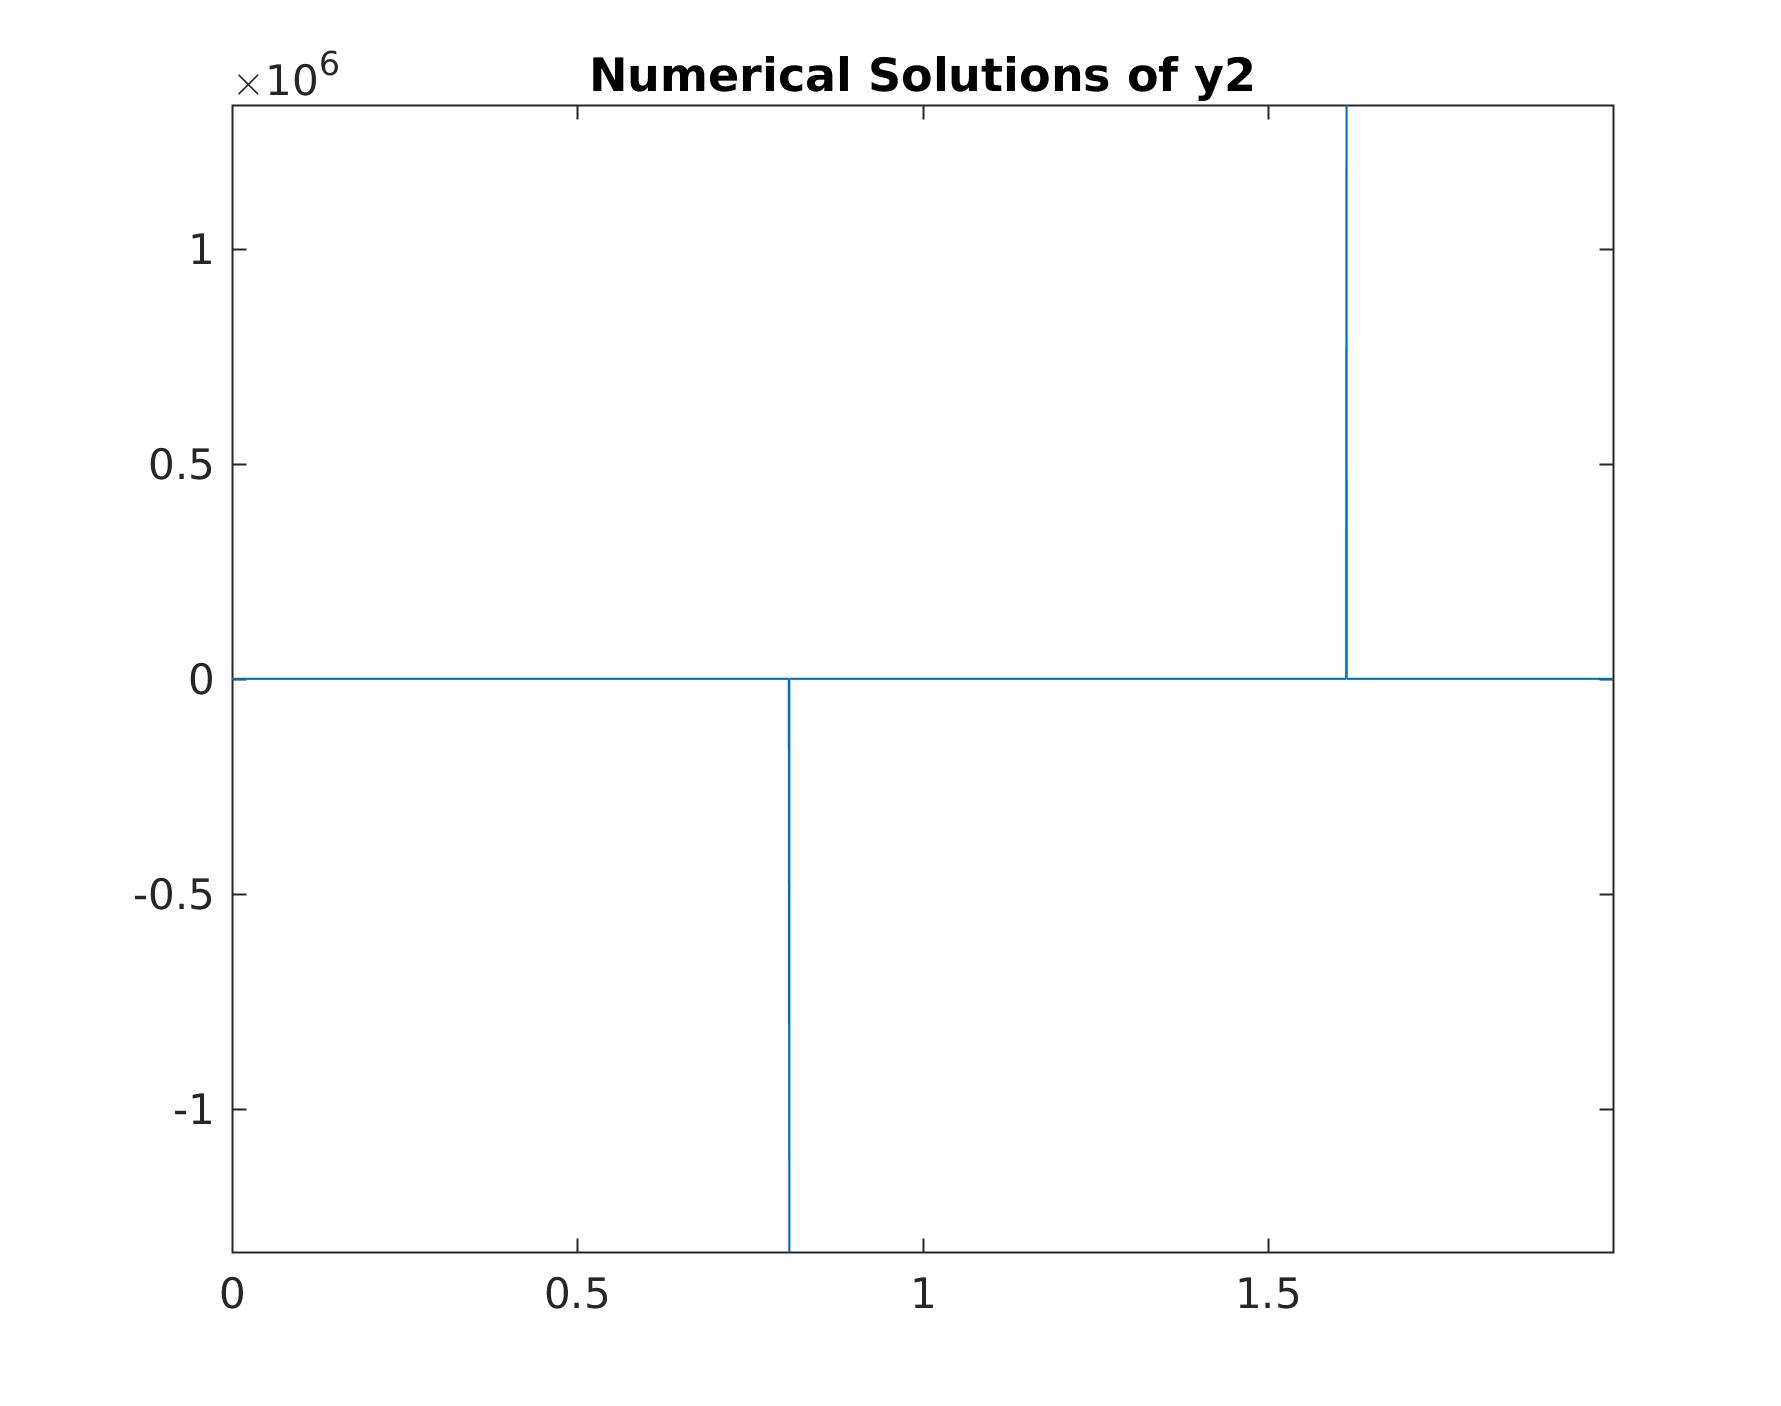
\includegraphics[scale=0.25]{fts_vdp_y2_1e-7_nl}
\caption{\textsc{Illustrations of Stiff Problems.}}
\end{figure}
\section{Introduction to Runge Kutta Methods}
A briefly introduction as follows,
\begin{itemize}
\item Classic, popular, well-known methods.
\item Are a family of explicit and implicit iterative methods for the approximate solutions of ODEs.
\item Extremely powerful tools for the solution of ODEs.
\item One can solve a majority of ODEs using a Runge Kutta scheme.
\end{itemize}
Hence, we now discover two part of this context in turns.
\begin{enumerate}
\item Explicit Runge Kutta methods. 
\item Implcit Runge Kutta methods.
\end{enumerate}




\part{Explicit Runge Kutta Methods}
\chapter{Introduction to Explicit Runge Kutta Methods}
We now consider the family of explicit Runge Kutta methods. The derivation of this scheme requires only Taylor series expansion. Although this approach really contains a lot of complicated computations, it is the most nature and naivest approach in this context. For alternative approaches, such as Butcher tree, see \cite{butcher}.
\section{Initial Value Problems}
The explicit Runge Kutta methods\index{explicit Runge Kutta methods} are an important family of iterative methods\index{iterative method} for the approximation of solutions of ODEs, that were developed around 1900 by the German mathematicians Carl Runge (1856-1927) and Martin. W. Kutta (1867-1944). Modern developments are mostly due to John Butcher in the 1960s.

We consider initial value problems\index{initial value problems} expressed in autonomous form\index{autonomous form}. Starting with the non-autonomous\index{non-autonomous form}, we assume that $f\left(x,y\right)$ is a continuous function with domain $\left[a,b\right]\times \mathbb{R}^n$ where $t \in \left[a,b\right]$ and $y\in \mathbb{R}^n$.

Consider the initial value problem\index{initial value problem}
\begin{align}
\label{1}
\dfrac{{dy\left( t \right)}}{{dt}} &= f\left( {t,y\left( t \right)} \right)\\
y\left( x_0 \right) &= {y_0}
\end{align}
where
\begin{align}
y\left( t \right) = {\left( {{y_1}\left( t \right),{y_2}\left( t \right), \ldots ,{y_n}\left( t \right)} \right)^T}
\end{align}
\begin{align}
f:\left[ {a,b} \right] \times {\mathbb{R}^n} \to {\mathbb{R}^n}
\end{align}

We assume that
\begin{align}
{\left\| {f\left( {t,{y_1}} \right) - f\left( {t,{y_2}} \right)} \right\|_{{L^2}\left( {{\mathbb{R}^n}} \right)}} \le L{\left\| {{y_1} - {y_2}} \right\|_{{L^2}\left( {{\mathbb{R}^n}} \right)}}
\end{align}
for all $t \in \left[ {a,b} \right],{y_1} \in {\mathbb{R}^n},{y_2} \in {\mathbb{R}^n}$.

Thus the initial value problem \eqref{1} has a unique solution.

For convenience, we write \eqref{1} briefly as
\begin{align}
y_t=f
\end{align}

Most efforts to increases the order of the explicit Runge Kutta methods have been accomplished by increasing the number of Taylor's series\index{Taylor's series} terms used and thus the number of functional evaluations, e.g. Butcher 1987, Gear 1971. The use of higher order derivative terms has been proposed for stiff problems\index{stiff problems}, e.g. Rosenbrock 1963, Enright 1974. Our method add higher order derivative terms to the explicit Runge Kutta $k_i$ terms ($i>1$) to achieve a higher order of accuracy\index{order of accuracy}. 

We are interested in a numerical approximation\index{numerical approximation} of the continuously differentiable solution\index{continuously differentiable solution of initial value problem} $y\left( t\right)$ of the initial value problem \eqref{1} over the time interval $t \in \left[ a,b\right]$.
\section{Mesh}
We subdivide the interval $\left[ {a,b} \right]$ into $M$ equal subintervals and select the mesh points $t_j$\index{mesh}
\begin{align}
{t_j} = a + jh,j = 0,1, \ldots ,M
\end{align}
where
\begin{align}
h = \dfrac{{b - a}}{M}
\end{align}
is called a step size\index{step size}.
\section{General Explicit Runge Kutta method}
The family of explicit Runge Kutta (abbr., RK) methods\index{family of explicit Runge Kutta methods} of the $m$th stage is given by
\begin{align}
\label{1.8}
{{y_{n + 1}}} = {{y_n}} + h\sum\limits_{i = 1}^s {{b_i}{k_i}} 
\end{align}
where
\begin{align}
\label{1.9}
{k_i} = f\left( {{\tau _i},{\eta _i}} \right),i = 1,2, \ldots ,s
\end{align}
and
\begin{align}
{\tau _i} &= {t_n} + {c_i}h
\end{align}
\begin{align}
{\eta _i} &= {y_n} + h\sum\limits_{j = 1}^{i - 1} {{a_{ij}}{k_j}} \\
 &= {y_n} + h\sum\limits_{j = 1}^{i - 1} {{a_{ij}}f\left( {{\tau _j},{\eta _j}} \right)} 
\end{align}

We use the notation
\begin{align}
{f_n}: = f\left( {{t_n},{y_n}} \right)
\end{align}

To specify a particular method, we need to provide the integer $s$ (the number of stages\index{number of stages}), and the coefficients $c_i,i=2,\ldots,s$, $a_{ij},1\le j<i\le m$ and $b_i,i=1,2,\ldots,s$.

These data are usually arranged in a so-called Butcher tableau\index{Butcher tableau} (after John C. Butcher)
\begin{align}
\begin{array}{*{20}{c}}
  0&\vline & {}&{}&{}&{}&{} \\ 
  {{c_2}}&\vline & {{a_{21}}}&{}&{}&{}&{} \\ 
  {{c_3}}&\vline & {{a_{31}}}&{{a_{32}}}&{}&{}&{} \\ 
   \vdots &\vline &  \vdots & \vdots & \ddots &{}&{} \\ 
  {{c_s}}&\vline & {{a_{s1}}}&{{a_{s2}}}& \cdots &{{a_{s,s - 1}}}&{} \\ 
\hline
  {}&\vline & {{b_1}}&{{b_2}}& \cdots &{{b_{s - 1}}}&{{b_s}} 
\end{array}
\end{align}
\section{Explicit Runge Kutta First Order Method}
We consider the explicit Runge Kutta first order method\index{explicit Runge Kutta first order method} here because it is very short and easy. There is no need to represent it into a separated chapter.

For $s=1$, \eqref{1.9} becomes
\begin{align}
{k_1} = f\left( {{t_n},{x_n}} \right)
\end{align}
and \eqref{1.9} becomes
\begin{align}
  {{y_{n + 1}}} &= {{y_n}} + h{b_1}{k_1}  \\
   &= {{y_n}} + h{b_1}{f_n}
\label{1.16}
\end{align}

On the other hand, the Taylor expansion yields
\begin{align}
{{y_{n + 1}}} &= {{y_n}} + h{\left. {{y_t}} \right|_{{t_n}}} + O\left( {{h^2}} \right)\\
 &= {{y_n}} + h{f_n} + O\left( {{h^2}} \right)
 \label{1.18}
\end{align}

Comparing \eqref{1.16} and \eqref{1.18}, we easily obtain 
\begin{align}
b_1=1
\end{align}
Hence, The Butcher table\index{Butcher table} in this case has the following form
\begin{align}
\begin{array}{*{20}{c}}
0&\vline& {}\\
\hline
{}&\vline& 1
\end{array}
\end{align}
\textbf{Remark 1.1.} The explicit Runge Kutta first order method\index{explicit Runge Kutta first order method} is equivalent to the explicit Euler's method\index{explicit Euler's method}. Note that the Euler's method\index{Euler's method} is of the first order of accuracy\index{first order of accuracy}. Hence, we get the name explicit Runge Kutta method of the \textit{first order} as above.  \hfill $\square$
\chapter{Explicit Runge Kutta Second Order Method}
In this chapter, we derive the formula of Runge Kutta second order method. Readers should notice the formulation and solving involving system of equations to this method. This contains the germs which will be essentially used to derive explicit Runge Kutta of higher orders later.
\section{Derivation of Explicit Runge Kutta Second Order Method}
To set up the explicit Runge Kutta second order method\index{explicit Runge Kutta second order method}, we need to do 4 steps.
\begin{enumerate}
\item Write down explicit Runge Kutta second order formula described by \eqref{1.8} and \eqref{1.9}.
\item Write down Taylor series expansion.
\item Compare the coefficients of two formulas above to obtain a system of equations. 
\item Solve the system of equation or find some its solutions.
\end{enumerate}
\textbf{Remark 2.1.} This process is also applied for explicit Runge Kutta methods of higher orders. Therefore, we can regard it as the standard process for derivation of the general Explicit Runge Kutta method\index{standard process for derivation of the general Explicit Runge Kutta method} in this context.\\

After these steps, with some solutions of the derived system of equations, we can simulate some initial value problems easily.
\subsection{Explicit Runge Kutta Second Order Formula}
For $s=2$, \eqref{1.9} becomes
\begin{align}
{k_1} &= {f_n}\\
{k_2} &= f\left( {{t_n} + {c_2}h,{y_n} + h{a_{21}}{f_n}} \right)
\end{align}
and \eqref{1.8} becomes
\begin{align}
{{y_{n + 1}}} &= {{y_n}} + h{b_1}{k_1} + h{b_2}{k_2}\\
 &= {{y_n}} + h{b_1}{f_n} + h{b_2}f\left( {{t_n} + {c_2}h,{y_n} + h{a_{21}}{f_n}} \right)
 \label{2.4}
\end{align}

Now we write down the Taylor series expansion $O\left(h^2\right)$ for ${k_2} $
\begin{align}
{k_2} &= f\left( {{t_n} + {c_2}h,{y_n} + h{a_{21}}{f_n}} \right)\\
 &= {f_n} + {c_2}h{f_t} + h{a_{21}}{f_n}{f_y} + O\left( {{h^2}} \right)
\label{2.6}
\end{align}

Inserting \eqref{2.6} into \eqref{2.4}, we obtain
\begin{align}
{{y_{n + 1}}} &= {{y_n}} + h{b_1}{f_n} + h{b_2}\left[ {{f_n} + {c_2}h{f_t} + h{a_{21}}{f_n}{f_y} + O\left( {{h^2}} \right)} \right]\\
 &= {{y_n}} + h\left( {{b_1} + {b_2}} \right){f_n} + {h^2}{b_2}{c_2}{f_t} + {h^2}{b_2}{a_{21}}{f_n}{f_y} + O\left( {{h^3}} \right)
 \label{2.8}
\end{align}
\subsection{Taylor Series Expansion Formula}
We need to compute $y_{tt}$ for Taylor series expansion below.
\begin{align}
{y_{tt}} &= \dfrac{{df}}{{dt}}\\
 &= \dfrac{{\partial f}}{{\partial t}}\dfrac{{\partial t}}{{\partial t}} + \dfrac{{\partial f}}{{\partial y}}\dfrac{{\partial y}}{{\partial t}}\\
 &= {f_t} + f{f_y}
\end{align}

Now we write down the Taylor series expansion of $y$ in the neighborhood of $t_n$ with $O\left(h^3\right)$.
\begin{align}
{{y_{n + 1}}} &= {{y_n}} + h{\left. {{y_t}} \right|_{{t_n}}} + \dfrac{{{h^2}}}{2}{\left. {{y_{tt}}} \right|_{{t_n}}} + O\left( {{h^3}} \right)\\
 &= {{y_n}} + h{f_n} + \dfrac{{{h^2}}}{2}{\left. {{y_{tt}}} \right|_{{t_n}}} + O\left( {{h^3}} \right)\\
 &= {{y_n}} + h{f_n} + \dfrac{{{h^2}}}{2}{\left. {\left( {{f_t} + f{f_y}} \right)} \right|_{{t_n}}} + O\left( {{h^3}} \right)\\
 &= {{y_n}} + h{f_n} + {\left. {\dfrac{{{h^2}}}{2}{f_t}} \right|_{{t_n}}} + \dfrac{{{h^2}}}{2}{f_n}{\left. {{f_y}} \right|_{{t_n}}} + O\left( {{h^3}} \right)
\label{2.11}
\end{align}\\
\\
\textbf{Remark 2.2.} \textit{(Important)} From here to later, if nothing is misunderstood, we can abbreviate notation ${f_{{t^\alpha }{y^\beta }}}$ for 
\begin{align}
{\left. {{f_{{t^\alpha }{y^\beta }}}} \right|_{{t_n}}}
\end{align}
in the Taylor series expansion.

For example, under this abbreviation, \eqref{2.11} can be rewritten briefly as
\begin{align}
\label{2.17}
{{y_{n + 1}}} = {{y_n}} + h{f_n} + \dfrac{{{h^2}}}{2}{f_t} + \dfrac{{{h^2}}}{2}{f_n}{f_y} + O\left( {{h^3}} \right)
\end{align}

This abbreviation reduces the complexity of the formulas in this context. As you will see later, this abbreviation is really essential.
\subsection{Derivation of System of Equations}
Return to our problem, as usual, comparing \eqref{2.8} and \eqref{2.17}, we obtain
\begin{align}
h{f_n}:1 &= {b_1} + {b_2}\\
{h^2}{f_t}:\dfrac{1}{2} &= {b_2}{c_2}\\
{h^2}{f_n}{f_y}:\dfrac{1}{2} &= {b_2}{a_{21}}
\end{align}

Hence, we obtain the system of equations
\begin{align}
{b_1} + {b_2} &= 1\label{2.21}\\
{b_2}{c_2} &= \dfrac{1}{2}\label{2.22}\\
{b_2}{a_{21}} &= \dfrac{1}{2}\label{2.23}
\end{align}
\subsection{Solutions of System of Equations}
We can solve the above system of equations easily. Here, the authors represent two solutions. The idea behind these two solutions will be use later for higher order explicit Runge Kutta method\index{higher order explicit Runge Kutta method}.\\
\\
\textsc{Solution 1.} The system involves four unknowns in three equations. Taking $b_2=\alpha$ is free variable. Due to \eqref{2.23} we must have $\alpha \ne 0$. Then we can easily obtain the general solution for \eqref{2.21}-\eqref{2.23} is
\begin{align}
{b_2} &= \alpha \\
{b_1} &= 1 - \alpha \\
{c_2} &= {a_{21}} = \dfrac{1}{{2\alpha }}
\label{2.26}
\end{align}
where $\alpha$ is an arbitrary real number.

Butcher tableau in this case becomes
\begin{align}
\begin{array}{*{20}{c}}
0&\vline& {}&{}\\
{\dfrac{1}{{2\alpha }}}&\vline& {\dfrac{1}{{2\alpha }}}&{}\\
\hline
{}&\vline& {1 - \alpha }&\alpha 
\end{array}
\end{align}
Done. \hfill $\square$\\
\\
\textsc{Solution 2.} Due to \eqref{2.21} and \eqref{2.22}, we must have $c_2 =a_{21}$. So, we can take
\begin{align}
c_2=a_{21}=\beta
\end{align}
as a free variable. And the remaining is very easy, we obtain 
\begin{align}
{b_1} &= 1 - \dfrac{1}{{2\beta }}\\
{b_2} &= \dfrac{1}{{2\beta }}\\
{c_2} &= {a_{21}} = \beta 
\end{align}
Butcher tableau in this case becomes
\begin{align}
\begin{array}{*{20}{c}}
0&\vline& {}&{}\\
\beta &\vline& \beta &{}\\
\hline
{}&\vline& {1 - \dfrac{1}{{2\beta }}}&{\dfrac{1}{{2\beta }}}
\end{array}
\end{align}
This Butcher tableau\index{Butcher tableau} appears in \cite{2}. \hfill $\square$\\
\\
\textbf{Remark 2.3.} Since explicit Runge Kutta second order\index{explicit Runge Kutta second order} is still simple, you can not see the differences between two solutions. With explicit Runge Kutta of higher order, you will see that the first choice of free variables is very important in entire solution.
\section{Some Cases}
We discuss two useful choices\\
\\
\textsc{Case $\alpha=\dfrac{1}{2}$.} In this case, \eqref{2.26} becomes
\begin{align}
{b_2} &= \dfrac{1}{2}\\
{b_1} &= \dfrac{1}{2}\\
{c_2} &= {a_{21}} = 1
\end{align}

The corresponding Butcher tableau reads
\begin{align}
\begin{array}{*{20}{c}}
0&\vline& {}&{}\\
1&\vline& 1&{}\\
\hline
{}&\vline& {\dfrac{1}{2}}&{\dfrac{1}{2}}
\end{array}
\end{align}

Thus, in this case the Explicit Runge Kutta method of second order\index{Explicit Runge Kutta method of second order} takes the form
\begin{align}
{{y_{n + 1}}} = {{y_n}} + \dfrac{h}{2}\left[ {{f_n} + f\left( {{t_n} + h,{y_n} + h{f_n}} \right)} \right]
\end{align}
and is equivalent to the Heun's method.\\
\\
\textsc{Case $\alpha =1$.} In this case, \eqref{2.26} becomes
\begin{align}
{b_2} &= 1\\
{b_1} &= 0\\
{c_2} &= {a_{21}} = \dfrac{1}{2}
\end{align}

The corresponding Butcher tableau reads
\begin{align}
\begin{array}{*{20}{c}}
0&\vline& {}&{}\\
{\dfrac{1}{2}}&\vline& {\dfrac{1}{2}}&{}\\
\hline
{}&\vline& 0&1
\end{array}
\end{align}

In this case Explicit Runge Kutta method of second order can be written as
\begin{align}
{{y_{n + 1}}} = {{y_n}} + hf\left( {{t_n} + \dfrac{h}{2},{y_n} + \dfrac{h}{2}{f_n}} \right)
\end{align}
and is called the RK2 method.\\
\\
Remember $\alpha \in \mathbb{R}^*$, so there is infinite many choices of solution for \eqref{2.21}-\eqref{2.23}.  \hfill $\square$


\chapter{Explicit Runge Kutta Third Order Method}
In this chapter, we continue to derive the formulation of Runge Kutta third order method. Notice that the amount of computations increase rapidly vs. the previous chapter.
\section{Derivation of Explicit Runge Kutta Third Order Method}
\subsection{Explicit Runge Kutta Third Order Formula}
For $s=3$, \eqref{1.9} becomes\index{explicit Runge Kutta third order method}
\begin{align}
{k_1} &= {f_n}\\
{k_2} &= f\left( {{t_n} + {c_2}h,{y_n} + h{a_{21}}{f_n}} \right)\\
{k_3} &= f\left( {{t_n} + {c_3}h,{y_n} + h{a_{31}}{k_1} + h{a_{32}}{k_2}} \right)\\
 &= f\left( {{t_n} + {c_3}h,{y_n} + h{a_{31}}{f_n} + h{a_{32}}f\left( {{t_n} + {c_2}h,{y_n} + h{a_{31}}{k_1} + h{a_{32}}{k_2}} \right)} \right)
\end{align}
and \eqref{1.8} becomes
\begin{align}
\label{3.5}
{{y_{n + 1}}} &= {{y_n}} + h{b_1}{k_1} + h{b_2}{k_2} + h{b_3}{k_3}
\end{align}

Now we write down the Taylor series expansion $O\left(h^3\right)$ for $k_2$.
\begin{align}
{k_2} &= f\left( {{t_n} + {c_2}h,{y_n} + h{a_{21}}{f_n}} \right)\\
 &= {f_n} + {c_2}h{f_t} + h{a_{21}}{f_n}{f_y} + {h^2}\dfrac{{c_2^2}}{2}{f_{tt}} + {h^2}{c_2}{a_{21}}{f_n}{f_{ty}} + {h^2}\dfrac{{a_{21}^2}}{2}f_n^2{f_{yy}} \\
 &+ O\left( {{h^3}} \right)
 \label{3.7}
\end{align}

And we also write down the Taylor series expansion $O\left(h^3\right)$ for $k_3$.
\begin{align}
{k_3} &= f\left( {{t_n} + {c_3}h,{y_n} + h{a_{31}}{f_n} + h{a_{32}}{k_2}} \right)\\
 &= {f_n} + {c_3}h{f_t} + h\left( {{a_{31}}{f_n} + {a_{32}}{k_2}} \right){f_y} \\
& + {h^2}\dfrac{{c_3^2}}{2}{f_{tt}} + {c_3}{h^2}\left( {{a_{31}}{f_n} + {a_{32}}{k_2}} \right){f_{ty}} + {h^2}\dfrac{{{{\left( {{a_{31}}{f_n} + {a_{32}}{k_2}} \right)}^2}}}{2}{f_{yy}} \\
&+ O\left( {{h^3}} \right)
 \label{3.10}
\end{align}

Inserting \eqref{3.7} into \eqref{3.10}
\begin{align}
{k_3} &= f\left( {{t_n} + {c_3}h,{y_n} + h{a_{31}}{f_n} + h{a_{32}}{k_2}} \right)\\
 &= {f_n} + {c_3}h{f_t} + h{a_{31}}{f_n}{f_y}\\
 &+ h{a_{32}}{f_y}\left( {{f_n} + h{c_2}{f_t} + h{a_{21}}{f_n}{f_y}} \right)\\
 &+ {h^2}\dfrac{{c_3^2}}{2}{f_{tt}} + {c_3}{h^2}\left( {{a_{31}}{f_n} + {a_{32}}{f_n}} \right){f_{ty}}\\
 &+ {h^2}\dfrac{{\left( {a_{31}^2f_n^2 + a_{32}^2f_n^2 + 2{a_{31}}{a_{32}}f_n^2} \right)}}{2}{f_{yy}}\\
 &+ O\left( {{h^3}} \right)
\end{align}

Collecting terms respect to exponents of $h$
\begin{align}
{k_3}  &= {f_n} + h\left( {{c_3}{f_t} + {a_{31}}{f_n}{f_y} + {a_{32}}{f_y}{f_n}} \right)\\
 &+ {h^2}\left( \begin{array}{l}
{a_{32}}{c_2}{f_t}{f_y} + {a_{21}}{a_{32}}{f_n}f_y^2 + \dfrac{{c_3^2}}{2}{f_{tt}}\\
 + {c_3}{a_{31}}{f_n}{f_{ty}} + {c_3}{a_{32}}{f_n}{f_{ty}} + \dfrac{{a_{31}^2}}{2}f_n^2{f_{yy}}\\
 + \dfrac{{a_{32}^2}}{2}f_n^2{f_{yy}} + {a_{31}}{a_{32}}f_n^2{f_{yy}}
\end{array} \right)\\
 &+ O\left( {{h^3}} \right)
 \label{3.19}
\end{align}

Inserting \eqref{3.10} and \eqref{3.19} into \eqref{3.5}
\begin{align}
{{y_{n + 1}}} &= {{y_n}} + h{b_1}{f_n}\\
 &+ h{b_2}\left( \begin{array}{l}
{f_n} + h{c_2}{f_t} + h{a_{21}}{f_n}{f_y} + {h^2}\dfrac{{c_2^2}}{2}{f_{tt}}\\
 + {h^2}{c_2}{a_{21}}{f_n}{f_{ty}} + {h^2}\dfrac{{a_{21}^2}}{2}f_n^2{f_{yy}}
\end{array} \right)\\
 &+ h{b_3}\left[ \begin{array}{l}
{f_n} + h\left( {{c_3}{f_t} + {a_{31}}{f_n}{f_y} + {a_{32}}{f_y}{f_n}} \right)\\
 + {h^2}\left( \begin{array}{l}
{a_{32}}{c_2}{f_t}{f_y} + {a_{21}}{a_{32}}{f_n}f_y^2 + \dfrac{{c_3^2}}{2}{f_{tt}}\\
 + {c_3}{a_{31}}{f_n}{f_{ty}} + {c_3}{a_{32}}{f_n}{f_{ty}} + \dfrac{{a_{31}^2}}{2}f_n^2{f_{yy}}\\
 + \dfrac{{a_{32}^2}}{2}f_n^2{f_{yy}} + {a_{31}}{a_{32}}f_n^2{f_{yy}}
\end{array} \right)
\end{array} \right]\\
 &+ O\left( {{h^4}} \right)
\end{align}

Collecting terms respect to exponents of $h$
\begin{align}
{{y_{n + 1}}} &= {{y_n}} + h\left( {{b_1}{f_n} + {b_2}{f_n} + {b_3}{f_n}} \right)\\
 &+ {h^2}\left( {{b_2}{c_2}{f_t} + {a_{21}}{b_2}{f_n}{f_y} + {b_3}{c_3}{f_t} + {a_{31}}{b_3}{f_n}{f_y} + {a_{32}}{b_3}{f_y}{f_n}} \right)\\
 &+ {h^3}\left( \begin{array}{l}
\dfrac{{{b_2}c_2^2}}{2}{f_{tt}} + {a_{21}}{b_2}{c_2}{f_n}{f_{ty}} + \dfrac{{a_{21}^2{b_2}}}{2}f_n^2{f_{yy}}\\
 + {a_{32}}{b_3}{c_2}{f_t}{f_y} + {a_{21}}{a_{32}}{b_3}{f_n}f_y^2 + \dfrac{{{b_3}c_3^2}}{2}{f_{tt}}\\
 + {a_{31}}{b_3}{c_3}{f_n}{f_{ty}} + {a_{32}}{b_3}{c_3}{f_n}{f_{ty}} + \dfrac{{a_{31}^2{b_3}}}{2}f_n^2{f_{yy}}\\
 + \dfrac{{a_{32}^2{b_3}}}{2}f_n^2{f_{yy}} + {a_{31}}{a_{32}}{b_3}f_n^2{f_{yy}}
\end{array} \right)\\
 &+ O\left( {{h^4}} \right)
 \label{3.27}
\end{align}
\subsection{Taylor Series Expansion Formula}
We need to compute $y_{ttt}$ for Taylor series expansion below.
\begin{align}
{y_{ttt}} &= \dfrac{d}{{dt}}\left( {{f_t} + f{f_y}} \right)\\
 &= {\left( {{f_t} + f{f_y}} \right)_t} + f{\left( {{f_t} + f{f_y}} \right)_y}\\
 &= {f_{tt}} + {f_t}{f_y} + f{f_{ty}} + f{f_{ty}} + ff_y^2 + {f^2}{f_{yy}}\\
 &= {f_{tt}} + {f_t}{f_y} + 2f{f_{ty}} + ff_y^2 + {f^2}{f_{yy}}
\end{align}

Now we write down the Taylor series expansion of $y$ in the neighborhood of $t_n$ with $O\left(h^4\right)$.
\begin{align}
 \label{3.34}
{{y_{n + 1}}} &= {{y_n}} + h{y_t} + \dfrac{{{h^2}}}{2}{y_{tt}} + \dfrac{{{h^3}}}{6}{y_{ttt}} + O\left( {{h^4}} \right)\\
 &= {{y_n}} + h{f_n} + \dfrac{{{h^2}}}{2}\left( {{f_t} + {f_n}{f_y}} \right)\\
 &+ \dfrac{{{h^3}}}{6}\left( {{f_{tt}} + {f_t}{f_y} + 2{f_n}{f_{ty}} + {f_n}f_y^2 + f_n^2{f_{yy}}} \right) + O\left( {{h^4}} \right)
 \label{3.36}
\end{align}
\subsection{Derivation of System of Equations}
Comparing \eqref{3.27} and \eqref{3.34}
\begin{align}
h{f_n}:1 &= {b_1} + {b_2} + {b_3}\\
{h^2}{f_t}:\dfrac{1}{2} &= {b_2}{c_2} + {b_3}{c_3}\\
{h^2}{f_n}{f_y}:\dfrac{1}{2} &= {a_{21}}{b_2} + {a_{31}}{b_3} + {a_{32}}{b_3}\\
{h^3}{f_{tt}}:\dfrac{1}{6} &= \dfrac{{{b_2}c_2^2}}{2} + \dfrac{{{b_3}c_3^2}}{2}\\
{h^3}{f_t}{f_y}:\dfrac{1}{6} &= {a_{32}}{b_3}{c_2}\\
{h^3}{f_n}{f_{ty}}:\dfrac{1}{3} &= {a_{21}}{b_2}{c_2} + {a_{31}}{b_3}{c_3} + {a_{32}}{b_3}{c_3}\\
{h^3}{f_n}f_y^2:\dfrac{1}{6} &= {a_{21}}{a_{32}}{b_3}\\
{h^3}f_n^2{f_{yy}}:\dfrac{1}{6} &= \dfrac{{a_{21}^2{b_2}}}{2} + \dfrac{{a_{31}^2{b_3}}}{2} + \dfrac{{a_{32}^2{b_3}}}{2} + {a_{31}}{a_{32}}{b_3}
\end{align}

Hence, we obtain the system of 8 equations with 8 unknowns.
\begin{align}
{b_1} + {b_2} + {b_3} &= 1\label{3.45}\\
{b_2}{c_2} + {b_3}{c_3} &= \dfrac{1}{2}\\
{b_2}{a_{21}} + {b_3}\left( {{a_{31}} + {a_{32}}} \right) &= \dfrac{1}{2}\\
{b_2}c_2^2 + {b_3}c_3^2 &= \dfrac{1}{3}\\
{b_3}{a_{32}}{c_2} &= \dfrac{1}{6}\label{3.49}\\
{b_2}{c_2}{a_{21}} + {b_3}{c_3}\left( {{a_{31}} + {a_{32}}} \right)& = \dfrac{1}{3}\\
{b_3}{a_{32}}{a_{21}} &= \dfrac{1}{6}\label{3.51}\\
{b_2}a_{21}^2 + {b_3}{\left( {{a_{31}} + {a_{32}}} \right)^2} &= \dfrac{1}{3}\label{3.52}
\end{align}
\subsection{Solutions of System of Equations}
We now solve the above system of equations in two different ways.\\
\\
\textsc{Solution 1.} We take $b_2=\alpha,b_3=\beta$ as two free variables, then 
\begin{align}
{b_1} = 1 - \alpha  - \beta 
\end{align}
our task remains to solve
\begin{align}
\alpha {c_2} + \beta {c_3} &= \dfrac{1}{2}\\
\alpha {a_{21}} + \beta \left( {{a_{31}} + {a_{32}}} \right) &= \dfrac{1}{2}\\
\alpha c_2^2 + \beta c_3^2 &= \dfrac{1}{3}\\
\beta {a_{32}}{c_2}& = \dfrac{1}{6}\label{3.57}\\
\alpha {c_2}{a_{21}} + \beta {c_3}\left( {{a_{31}} + {a_{32}}} \right) &= \dfrac{1}{3}\\
\beta {a_{32}}{a_{21}} &= \dfrac{1}{6}\label{3.59}\\
\alpha a_{21}^2 + \beta {\left( {{a_{31}} + {a_{32}}} \right)^2} &= \dfrac{1}{3}
\end{align}
We can solve $c_2$ and $c_3$ by using two equations
\begin{align}
\alpha {c_2} + \beta {c_3} &= \dfrac{1}{2}\label{3.61}\\
\alpha c_2^2 + \beta c_3^2 &= \dfrac{1}{3}\label{3.62}
\end{align}
Since \eqref{3.59}, we must have $\beta \ne 0$.

Then we can take ${c_3} = \dfrac{1}{{2\beta }} - \dfrac{\alpha }{\beta }{c_2}$ from \eqref{3.61} and insert into \eqref{3.62} to obtain the following equation respect to $c_2$.
\begin{align}
\label{3.63}
12\alpha \left( {\alpha  + \beta } \right)c_2^2 - 12\alpha {c_2} + 3 - 4\beta  = 0
\end{align}
Consider two following cases.
\begin{enumerate}
\item \textbf{Case $\alpha \left( {\alpha  + \beta } \right)=0$.} Consider two subcases.
\begin{enumerate}
\item \textbf{Case $\alpha=0$.} Then we have immediately
\begin{align}
\beta  &= \dfrac{3}{4}\\
{c_3} &= \dfrac{2}{3}\\
b_1 &=\dfrac{1}{4}
\end{align}
and the system of equations remains
\begin{align}
{a_{31}} + {a_{32}} &= \dfrac{2}{3}\\
{a_{32}}{c_2} &= \dfrac{2}{9}\\
\dfrac{3}{4}{a_{32}}{a_{21}} &= \dfrac{1}{6}
\end{align}
To solve this remaining system of equations, we can take $a_{32}=\gamma \ne 0$ as a free variable. Then
\begin{align}
{a_{31}} &= \dfrac{2}{3} - \gamma \\
{c_2} &= \dfrac{2}{{9\gamma }}\\
{a_{21}} &=\dfrac{2}{{9\gamma }}
\end{align}
Hence, we obtain the solutions
\begin{align}
{b_1} &= \dfrac{1}{4}\\
{b_2} &= 0\\
{b_3} &= \dfrac{3}{4}\\
{c_2} &= \dfrac{2}{{9\gamma }}\\
{c_3} &= \dfrac{2}{3}\\
{a_{21}} &= \dfrac{2}{{9\gamma }}\\
{a_{31}} &= \dfrac{2}{3} - \gamma \\
{a_{32}} &= \gamma 
\end{align}
where $\gamma$ is an arbitrary nonzero real number, in this subcase.

Butcher tableau becomes
\begin{align}
\begin{array}{*{20}{c}}
0&\vline& {}&{}&{}\\
{\dfrac{2}{{9\gamma }}}&\vline& {\dfrac{2}{{9\gamma }}}&{}&{}\\
{\dfrac{2}{3}}&\vline& {\dfrac{2}{3} - \gamma }&\gamma &{}\\
\hline
{}&\vline& {\dfrac{1}{4}}&0&{\dfrac{3}{4}}
\end{array}
\end{align}
\item \textbf{Case $\alpha + \beta =0,\alpha \ne 0$.} Then we have immediately
\begin{align}
{b_1} &= 1\\
{b_2} &= \alpha \\
{b_3} &=  - \alpha \\
{c_2} &= \dfrac{1}{3} + \dfrac{1}{{4\alpha }}
\end{align}
and the system of equations remains
\begin{align}
{c_2} - {c_3} &= \dfrac{1}{{2\alpha }}\\
{a_{21}} - \left( {{a_{31}} + {a_{32}}} \right) &= \dfrac{1}{{2\alpha }}\\
c_2^2 - c_3^2 &= \dfrac{1}{{3\alpha }}\\
{a_{32}}{c_2} &=  - \dfrac{1}{{6\alpha }}\\
{c_2}{a_{21}} - {c_3}\left( {{a_{31}} + {a_{32}}} \right) &= \dfrac{1}{{3\alpha }}\\
{a_{32}}{a_{21}}& =  - \dfrac{1}{{6\alpha }}\\
a_{21}^2 - {\left( {{a_{31}} + {a_{32}}} \right)^2} &= \dfrac{1}{{3\alpha }}
\end{align}
We again have immediately
\begin{align}
{c_3} &= \dfrac{1}{3} - \dfrac{1}{{4\alpha }}\\
{a_{32}} &=  - \dfrac{2}{{4\alpha  + 3}}\\
{a_{21}} &= \dfrac{1}{3} + \dfrac{1}{{4\alpha }}\\
{a_{31}} &= \dfrac{{16{\alpha ^2} + 24\alpha  - 9}}{{12\alpha \left( {4\alpha  + 3} \right)}}
\end{align}
Hence, we obtain the solution
\begin{align}
{b_1} &= 1\\
{b_2} &= \alpha \\
{b_3} &=  - \alpha \\
{c_2}& = \dfrac{1}{3} + \dfrac{1}{{4\alpha }}\\
{c_3} &= \dfrac{1}{3} - \dfrac{1}{{4\alpha }}\\
{a_{21}} &= \dfrac{1}{3} + \dfrac{1}{{4\alpha }}\\
{a_{31}} &= \dfrac{{16{\alpha ^2} + 24\alpha  - 9}}{{12\alpha \left( {4\alpha  + 3} \right)}}\\
{a_{32}} &=  - \dfrac{2}{{4\alpha  + 3}}
\end{align}
where $\alpha$ is an arbitrary nonzero real number, in this subcase.

Butcher tableau\index{Butcher tableau} becomes
\begin{align}
\begin{array}{*{20}{c}}
0&\vline& {}&{}&{}\\
{\dfrac{1}{3} + \dfrac{1}{{4\alpha }}}&\vline& {\dfrac{1}{3} + \dfrac{1}{{4\alpha }}}&{}&{}\\
{\dfrac{1}{3} - \dfrac{1}{{4\alpha }}}&\vline& {\dfrac{{16{\alpha ^2} + 24\alpha  - 9}}{{12\alpha \left( {4\alpha  + 3} \right)}}}&{ - \dfrac{2}{{4\alpha  + 3}}}&{}\\
\hline
{}&\vline& 1&\alpha &{ - \alpha }
\end{array}
\end{align}
\end{enumerate}
\item \textbf{Case $\alpha \left( {\alpha  + \beta } \right)\ne 0$.} \eqref{3.63} is a quadratic equation respect to $c_2$.

Computing the determinant of \eqref{3.63}
\begin{align}
\Delta ' &= 36{\alpha ^2} + 12\alpha \left( {\alpha  + \beta } \right)\left( {4\beta  - 3} \right)\\
 &= 12\alpha \beta \left( {4\alpha  + 4\beta  - 3} \right)
\end{align}
Hence, we have to make the assumption 
\begin{align}
\alpha \beta \left( {4\alpha  + 4\beta  - 3} \right) \ge 0
\end{align}
so that \eqref{3.63} has roots in this case.

Under this assumption, \eqref{3.63} have two roots
\begin{align}
{c_2} = \dfrac{{3\alpha  \pm \sqrt {3\alpha \beta \left( {4\alpha  + 4\beta  - 3} \right)} }}{{6\alpha \left( {\alpha  + \beta } \right)}}
\end{align}
Consider two subcases respect to $c_2$.
\begin{enumerate}
\item \textbf{Case ${c_2} = \dfrac{{3\alpha  + \sqrt {3\alpha \beta \left( {4\alpha  + 4\beta  - 3} \right)} }}{{6\alpha \left( {\alpha  + \beta } \right)}}$.}
We easily solve the remaining system of equations to get
\begin{align}
{b_1} &= 1 - \alpha  - \beta \\
{b_2} &= \alpha \\
{b_3} &= \beta \\
{c_2} &= \dfrac{{3\alpha  + \sqrt {3\alpha \beta \left( {4\alpha  + 4\beta  - 3} \right)} }}{{6\alpha \left( {\alpha  + \beta } \right)}}\\
{c_3} &= \dfrac{{3\beta  - \sqrt {3\alpha \beta \left( {4\alpha  + 4\beta  - 3} \right)} }}{{6\beta \left( {\alpha  + \beta } \right)}}\\
{a_{21}} &= \dfrac{{3\alpha  + \sqrt {3\alpha \beta \left( {4\alpha  + 4\beta  - 3} \right)} }}{{6\alpha \left( {\alpha  + \beta } \right)}}\\
{a_{31}} &= \dfrac{1}{{2\beta }} - \dfrac{{3\alpha  + \sqrt {3\alpha \beta \left( {4\alpha  + 4\beta  - 3} \right)} }}{{6\beta \left( {\alpha  + \beta } \right)}} \\
&- \dfrac{{\alpha \left( {\alpha  + \beta } \right)}}{{\beta \left( {3\alpha  + \sqrt {3\alpha \beta \left( {4\alpha  + 4\beta  - 3} \right)} } \right)}}\\
{a_{32}} &= \dfrac{{\alpha \left( {\alpha  + \beta } \right)}}{{\beta \left( {3\alpha  + \sqrt {3\alpha \beta \left( {4\alpha  + 4\beta  - 3} \right)} } \right)}}
\end{align}
Butcher tableau\index{Butcher tableau} reads all obtained coefficients.
\item \textbf{Case ${c_2} = \dfrac{{3\alpha  - \sqrt {3\alpha \beta \left( {4\alpha  + 4\beta  - 3} \right)} }}{{6\alpha \left( {\alpha  + \beta } \right)}}$.} 
We also easily solve the remaining system of equations to get
\begin{align}
{b_1} &= 1 - \alpha  - \beta \\
{b_2} &= \alpha \\
{b_3} &= \beta \\
{c_2} &= \dfrac{{3\alpha  - \sqrt {3\alpha \beta \left( {4\alpha  + 4\beta  - 3} \right)} }}{{6\alpha \left( {\alpha  + \beta } \right)}}\\
{c_3} &= \dfrac{{3\beta  + \sqrt {3\alpha \beta \left( {4\alpha  + 4\beta  - 3} \right)} }}{{6\beta \left( {\alpha  + \beta } \right)}}\\
{a_{21}} &= \dfrac{{3\alpha  - \sqrt {3\alpha \beta \left( {4\alpha  + 4\beta  - 3} \right)} }}{{6\alpha \left( {\alpha  + \beta } \right)}}\\
{a_{31}} &= \dfrac{1}{{2\beta }} - \dfrac{{3\alpha  - \sqrt {3\alpha \beta \left( {4\alpha  + 4\beta  - 3} \right)} }}{{6\beta \left( {\alpha  + \beta } \right)}}\\
 &- \dfrac{{\alpha \left( {\alpha  + \beta } \right)}}{{\beta \left( {3\alpha  - \sqrt {3\alpha \beta \left( {4\alpha  + 4\beta  - 3} \right)} } \right)}}\\
{a_{32}} &= \dfrac{{\alpha \left( {\alpha  + \beta } \right)}}{{\beta \left( {3\alpha  - \sqrt {3\alpha \beta \left( {4\alpha  + 4\beta  - 3} \right)} } \right)}}
\end{align}
Butcher tableau reads all obtained coefficients.
\end{enumerate}
\end{enumerate}
We have solved the system of equations \eqref{3.45}-\eqref{3.52} completely. \hfill $\square$\\
\\
\textbf{Remark 3.1.} In the first solution, we have used $b_2$ and $b_3$ as two free variables. This choice makes square roots appear in the solutions. This is quite easy to understand. Because of choice of $b_2,b_3$ as free variables, we have to solve a quadratic equation. This quadratic equation make square roots appear obviously.\\

Now, we solve our system of equation by alternative ways. The idea is very simple. It is just a matter of the first choice. More explicitly, instead of choosing $b_2,b_3$ as two free variables, we will choose $c_2,c_3$ as two free variables. Let us see the differences between two solutions through the following second one.\\
\\
\textsc{Solution 2.} We take ${c_2} = \alpha ,{c_3} = \beta $ as two free variables and focus on the following two equations of our system of equations.
\begin{align}
{b_2}{c_2} + {b_3}{c_3} &= \dfrac{1}{2}\label{3.128}\\
{b_2}c_2^2 + {b_3}c_3^3 &= \dfrac{1}{3}\label{3.129}
\end{align}
We consider two cases respect to $c_2$ and $c_3$.
\begin{enumerate}
\item \textbf{Case $c_2=c_3=\alpha$.} Due to \eqref{3.57}, we must have $\alpha \ne 0$. Then the above sub-system of equations becomes
\begin{align}
{b_2} + {b_3} &= \dfrac{1}{{2\alpha }}\\
{b_2} + {b_3} &= \dfrac{1}{{3{\alpha ^2}}}
\end{align}
Hence
\begin{align}
c_2=c_3 =\alpha =\dfrac{2}{3}
\end{align}
The remaining system of equations is
\begin{align}
{b_1} + {b_2} + {b_3} &= 1\\
{b_2} + {b_3} &= \dfrac{3}{4}\\
{b_2}{a_{21}} + {b_3}\left( {{a_{31}} + {a_{32}}} \right) &= \dfrac{1}{2}\\
{b_3}{a_{32}} &= \dfrac{1}{4}\\
{b_3}{a_{32}}{a_{21}} &= \dfrac{1}{6}\\
{b_2}a_{21}^2 + {b_3}{\left( {{a_{31}} + {a_{32}}} \right)^2} &= \dfrac{1}{3}
\end{align}
We obtain immediately
\begin{align}
{b_1} &= \dfrac{1}{4}\\
{a_{21}} &= \dfrac{2}{3}
\end{align}
and the remaining system of equations is
\begin{align}
{b_2} + {b_3} &= \dfrac{3}{4}\label{3.141}\\
\dfrac{2}{3}{b_2} + {b_3}\left( {{a_{31}} + {a_{32}}} \right) &= \dfrac{1}{2}\label{3.142}\\
{b_3}{a_{32}} &= \dfrac{1}{4}\\
\dfrac{4}{9}{b_2} + {b_3}{\left( {{a_{31}} + {a_{32}}} \right)^2} &= \dfrac{1}{3}\label{3.144}
\end{align}
We now choose $b_3=\gamma$ then
\begin{align}
{b_2} &= \dfrac{3}{4} - \gamma \\
{a_{31}} &= \dfrac{2}{3} - \dfrac{1}{{4\gamma }}\\
{a_{32}} &= \dfrac{1}{{4\gamma }}
\end{align}
Therefore,
\begin{align}
{c_2} &= \dfrac{2}{3}\\
{c_3} &= \dfrac{2}{3}\\
{b_1} &= \dfrac{1}{4}\\
{b_2} &= \dfrac{3}{4} - \gamma \\
{b_3} &= \gamma \\
{a_{21}} &= \dfrac{2}{3}\\
{a_{31}} &= \dfrac{2}{3} - \dfrac{1}{{4\gamma }}\\
{a_{32}} &= \dfrac{1}{{4\gamma }}
\end{align}
where $\gamma$ is an arbitrary  nonzero real number, is the solution of \eqref{3.45}-\eqref{3.52} in this case.
\item \textbf{Case $c_2 \ne c_3$.} Due to \eqref{3.49} and \eqref{3.51}, we have immediately
\begin{align}
a_{21}=c_2=\alpha
\end{align}

Due to \eqref{3.128} and \eqref{3.129}, we obtain
\begin{align}
{b_2} &= \dfrac{{3\beta  - 2}}{{6\alpha \left( {\beta  - \alpha } \right)}}\\
{b_3} &= \dfrac{{3\alpha  - 2}}{{6\beta \left( {\alpha  - \beta } \right)}}
\end{align}
Hence, 
\begin{align}
{b_1} = \dfrac{{6\alpha \beta  - 3\alpha  - 3\beta  + 2}}{{6\alpha \beta }}
\end{align}
The remaining system of equations is
\begin{align}
\dfrac{{3\beta  - 2}}{{6\alpha \left( {\beta  - \alpha } \right)}}\alpha  + \dfrac{{3\alpha  - 2}}{{6\beta \left( {\alpha  - \beta } \right)}}\left( {{a_{31}} + {a_{32}}} \right) &= \dfrac{1}{2}\\
\dfrac{{3\alpha  - 2}}{{6\beta \left( {\alpha  - \beta } \right)}}{a_{32}}\alpha &= \dfrac{1}{6}\\
\dfrac{{3\beta  - 2}}{{6\left( {\beta  - \alpha } \right)}}\alpha  + \dfrac{{3\alpha  - 2}}{{6\left( {\alpha  - \beta } \right)}}\left( {{a_{31}} + {a_{32}}} \right) &= \dfrac{1}{3}\\
\dfrac{{3\beta  - 2}}{{6\alpha \left( {\beta  - \alpha } \right)}}{\alpha ^2} + \dfrac{{3\alpha  - 2}}{{6\beta \left( {\alpha  - \beta } \right)}}{\left( {{a_{31}} + {a_{32}}} \right)^2} &= \dfrac{1}{3}
\end{align}
We easily solve this and obtain
\begin{align}
{a_{21}} &= \alpha \\
{a_{31}} &= \beta  - \dfrac{{\beta \left( {\alpha  - \beta } \right)}}{{\alpha \left( {3\alpha  - 2} \right)}}\\
{a_{32}} &= \dfrac{{\beta \left( {\alpha  - \beta } \right)}}{{\alpha \left( {3\alpha  - 2} \right)}}
\end{align}
Therefore, 
\begin{align}
{c_2} &= \alpha \\
{c_3} &= \beta \\
{b_1} &= \dfrac{{6\alpha \beta  - 3\alpha  - 3\beta  + 2}}{{6\alpha \beta }}\\
{b_2} &= \dfrac{{3\beta  - 2}}{{6\alpha \left( {\beta  - \alpha } \right)}}\\
{b_3} &= \dfrac{{3\alpha  - 2}}{{6\beta \left( {\alpha  - \beta } \right)}}\\
{a_{21}} &= \alpha \\
{a_{31}} &= \beta  - \dfrac{{\beta \left( {\alpha  - \beta } \right)}}{{\alpha \left( {3\alpha  - 2} \right)}}\\
{a_{32}} &= \dfrac{{\beta \left( {\alpha  - \beta } \right)}}{{\alpha \left( {3\alpha  - 2} \right)}}
\end{align}
where $\alpha \ne \beta,\alpha \ne \dfrac{2}{3}$ are two arbitrary nonzero real numbers, is the solution of \eqref{3.45}-\eqref{3.52} in this case.
\end{enumerate}
We have solved \eqref{3.45}-\eqref{3.52} completely. \hfill $\square$\\
\\
\textbf{Remark 3.2.} In the second solution, $n$th roots do not appear in the solution because we does not need to solve any polynomial equations\index{polynomial equations}. Since this way is more easy and effective, it will be used for explicit Runge Kutta method of higher orders.
\section{Some Cases}
We consider some cases of explicit Runge Kutta third order method\index{explicit Runge Kutta third order method} respect to some solutions of its associated system of equations.\\
\\
\textsc{Case $\alpha  = \dfrac{2}{3},\beta  = \dfrac{1}{6}$.}\\
We use case \textbf{2.(b)} above to obtain
\begin{align}
\begin{array}{*{20}{c}}
0&\vline& {}&{}&{}\\
{\dfrac{1}{2}}&\vline& {\dfrac{1}{2}}&{}&{}\\
1&\vline& { - 1}&2&{}\\
\hline
{}&\vline& {\dfrac{1}{6}}&{\dfrac{2}{3}}&{\dfrac{1}{6}}
\end{array}
\end{align}
This Butcher tableau\index{Butcher tableau} appears in \cite{3} - Kutta's third order method\index{Kutta's third order method} and in \cite{butcher}, p.82.\\
\\
\textsc{Case $\alpha  = \dfrac{3}{8},\beta  = \dfrac{3}{8}$.}
\begin{align}
\begin{array}{*{20}{c}}
0&\vline& {}&{}&{}\\
{\dfrac{2}{3}}&\vline& {\dfrac{2}{3}}&{}&{}\\
{\dfrac{2}{3}}&\vline& 0&{\dfrac{2}{3}}&{}\\
\hline
{}&\vline& {\dfrac{1}{4}}&{\dfrac{3}{8}}&{\dfrac{3}{8}}
\end{array}
\end{align}
This Butcher tableau appears in \cite{butcher}, p.82.\\
\\
\textsc{Case $\alpha  = \dfrac{3}{4},\beta  = \dfrac{1}{4}$.}

\begin{align}
\begin{array}{*{20}{c}}
0&\vline& {}&{}&{}\\
{\dfrac{2}{3}}&\vline& {\dfrac{2}{3}}&{}&{}\\
0&\vline& { - 1}&1&{}\\
\hline
{}&\vline& 0&{\dfrac{3}{4}}&{\dfrac{1}{4}}
\end{array}
\end{align}
This Butcher tableau appears in \cite{butcher}, p.82.  \hfill $\square$
\chapter{Explicit Runge Kutta Fourth Order Method}
We continue to derive the formulation of Runge Kutta fourth order method. The amount of complicated computations continues to increase rapidly.
\section{Derivation of Explicit Runge Kutta Fourth Order Method}
\subsection{Explicit Runge Kutta Fourth Order Formula}
For $s=4$, \eqref{1.9} becomes\index{Explicit Runge Kutta fourth order method}
\begin{align}
{k_1} &= {f_n}\\
{k_2} &= f\left( {{t_n} + {c_2}h,{y_n} + h{a_{21}}{f_n}} \right)\\
{k_3} &= f\left( {{t_n} + {c_3}h,{y_n} + h{a_{31}}{f_n} + h{a_{32}}{k_2}} \right)\\
{k_4} &= f\left( {{t_n} + {c_4}h,{y_n} + h{a_{41}}{f_n} + h{a_{42}}{k_2} + h{a_{43}}{k_3}} \right)
\end{align}

and \eqref{1.8} becomes
\begin{align}
\label{4.5}
{{y_{n + 1}}} = {{y_n}} + h{b_1}{k_1} + h{b_2}{k_2} + h{b_3}{k_3} + h{b_4}{k_4} 
\end{align}

Now we write down the Taylor series expansion $O\left(h^4\right)$ for $k_2$.
\begin{align}
{k_2} &= f\left( {{t_n} + {c_2}h,{y_n} + h{a_{21}}{f_n}} \right)\\
 &= {f_n} + h{c_2}{f_t} + h{a_{21}}{f_n}{f_y} + {h^2}\dfrac{{c_2^2}}{2}{f_{tt}} + {h^2}{a_{21}}{c_2}{f_n}{f_{ty}} + {h^2}\dfrac{{a_{21}^2}}{2}f_n^2\\
 &+ {h^3}\dfrac{{c_2^3}}{6}{f_{ttt}} + {h^3}\dfrac{{{a_{21}}c_2^2}}{2}{f_n}{f_{tty}} + {h^3}\dfrac{{a_{21}^2{c_2}}}{2}f_n^2{f_{tyy}} + {h^3}\dfrac{{a_{21}^3}}{6}f_n^3{f_{yyy}} + O\left( {{h^4}} \right)\\
 &= {f_n} + h\left( {{c_2}{f_t} + {a_{21}}{f_n}{f_y}} \right) + {h^2}\left( {\dfrac{{c_2^2}}{2}{f_{tt}} + {a_{21}}{c_2}{f_n}{f_{ty}} + \dfrac{{a_{21}^2}}{2}f_n^2} \right)\\
 &+ {h^3}\left( {\dfrac{{c_2^3}}{6}{f_{ttt}} + \dfrac{{{a_{21}}c_2^2}}{2}{f_n}{f_{tty}} + \dfrac{{a_{21}^2{c_2}}}{2}f_n^2{f_{tyy}} + \dfrac{{a_{21}^3}}{6}f_n^3{f_{yyy}}} \right) + O\left( {{h^4}} \right)
 \label{4.10}
\end{align}

We write down the Taylor series expansion $O\left(h^4\right)$ for $k_3$.
\begin{align}
{k_3} &= f\left( {{t_n} + {c_3}h,{y_n} + h{a_{31}}{f_n} + h{a_{32}}{k_2}} \right)\\
 &= {f_n} + h{c_3}{f_t} + h\left( {{a_{31}}{f_n} + {a_{32}}{k_2}} \right){f_y}\\
 &+ {h^2}\dfrac{{c_3^2}}{2}{f_{tt}} + {h^2}{c_3}\left( {{a_{31}}{f_n} + {a_{32}}{k_2}} \right){f_{ty}} + \dfrac{1}{2}{h^2}{\left( {{a_{31}}{f_n} + {a_{32}}{k_2}} \right)^2}{f_{yy}}\\
 &+ \dfrac{{c_3^3{h^3}}}{6}{f_{ttt}} + \dfrac{{{h^3}c_3^2}}{2}\left( {{a_{31}}{f_n} + {a_{32}}{k_2}} \right){f_{tty}} + \dfrac{{{h^3}{c_3}}}{2}{\left( {{a_{31}}{f_n} + {a_{32}}{k_2}} \right)^2}{f_{tyy}}\\
 &+ \dfrac{{{h^3}}}{6}{\left( {{a_{31}}{f_n} + {a_{32}}{k_2}} \right)^3}{f_{yyy}} + O\left( {{h^4}} \right)
 \label{4.15}
\end{align}

Inserting \eqref{4.10} into \eqref{4.15}
\begin{align}
{k_3} &= {f_n} + h{c_3}{f_t} + h{a_{31}}{f_n}{f_y}\\
 &+ h{a_{32}}{f_y}\left[ {{f_n} + h\left( {{c_2}{f_t} + {a_{21}}{f_n}{f_y}} \right) + {h^2}\left( {\dfrac{{c_2^2}}{2}{f_{tt}} + {a_{21}}{c_2}{f_n}{f_{ty}} + \dfrac{{a_{21}^2}}{2}f_n^2} \right)} \right]\\
 &+ \dfrac{{{h^2}c_3^2}}{2}{f_{tt}} + {h^2}{c_3}{a_{31}}{f_n}{f_{ty}} + {h^2}{c_3}{a_{32}}{f_{ty}}\left[ {{f_n} + h\left( {{c_2}{f_t} + {a_{21}}{f_n}{f_y}} \right)} \right]\\
 &+ \dfrac{{{h^2}}}{2}a_{31}^2f_n^2{f_{yy}} + \dfrac{{{h^2}}}{2}2{a_{31}}{a_{32}}{f_n}{f_{yy}}\left[ {{f_n} + h\left( {{c_2}{f_t} + {a_{21}}{f_n}{f_y}} \right)} \right]\\
 &+ \dfrac{{{h^2}}}{2}a_{32}^2{f_{yy}}{\left[ {{f_n} + h\left( {{c_2}{f_t} + {a_{21}}{f_n}{f_y}} \right)} \right]^2}\\
 &+ \dfrac{{c_3^3{h^3}}}{6}{f_{ttt}} + \dfrac{{{h^3}c_3^2}}{2}\left( {{a_{31}}{f_n} + {a_{32}}{f_n}} \right){f_{tty}}\\
 &+ \dfrac{{{h^3}{c_3}}}{2}\left( {a_{31}^2f_n^2 + 2{a_{31}}{a_{32}}f_n^2 + a_{32}^2f_n^2} \right){f_{tyy}}\\
 &+ \dfrac{{{h^3}}}{6}\left( {a_{31}^3f_n^3 + 3a_{31}^2{a_{32}}f_n^3 + 3{a_{31}}a_{32}^2f_n^3 + a_{32}^3f_n^3} \right){f_{yyy}} + O\left( {{h^4}} \right)
\end{align}

Collecting terms respect to exponents of $h$
\begin{align}
{k_3} &= {f_n} + h\left( {{c_3}{f_t} + {a_{31}}{f_n}{f_y} + {a_{32}}{f_n}{f_y}} \right)\\
 &+ {h^2}\left( \begin{array}{l}
{a_{32}}{c_2}{f_t}{f_y} + {a_{21}}{a_{32}}{f_n}f_y^2 + \dfrac{{c_3^2}}{2}{f_{tt}} + {a_{31}}{c_3}{f_n}{f_{ty}}\\
 + {c_3}{a_{32}}{f_n}{f_{ty}} + \dfrac{{a_{31}^2}}{2}f_n^2{f_{yy}} + {a_{31}}{a_{32}}f_n^2{f_{yy}} + \dfrac{{a_{32}^2}}{2}f_n^2{f_{yy}}
\end{array} \right)\\
 &+ {h^3}\left( \begin{array}{l}
\dfrac{{{a_{32}}c_2^2}}{2}{f_y}{f_{tt}} + {a_{32}}{a_{21}}{c_2}{f_n}{f_y}{f_{ty}} + \dfrac{{a_{21}^2{a_{32}}}}{2}f_n^2{f_y}\\
 + {a_{32}}{c_2}{c_3}{f_t}{f_{ty}} + {a_{21}}{a_{32}}{c_3}{f_n}{f_y}{f_{ty}} + {a_{31}}{a_{32}}{c_2}{f_n}{f_t}{f_{yy}}\\
 + {a_{21}}{a_{31}}{a_{32}}f_n^2{f_y}{f_{yy}} + a_{32}^2{c_2}{f_n}f{f_{yy}}_t + {a_{21}}a_{32}^2f_n^2{f_y}{f_{yy}}\\
 + \dfrac{{c_3^3}}{6}{f_{ttt}} + \dfrac{{{a_{31}}c_3^2}}{2}{f_n}{f_{tty}} + \dfrac{{{a_{32}}c_3^2}}{2}{f_n}{f_{tty}} + \dfrac{{a_{31}^2{c_3}}}{2}f_n^2{f_{tyy}}\\
 + {a_{31}}{a_{32}}{c_3}f_n^2{f_{tyy}} + \dfrac{{a_{32}^2{c_3}}}{2}f_n^2{f_{tyy}} + \dfrac{{a_{31}^3}}{6}f_n^3{f_{yyy}}\\
 + \dfrac{{a_{31}^2{a_{32}}}}{2}f_n^3{f_{yyy}} + \dfrac{{{a_{31}}a_{32}^2}}{2}f_n^3{f_{yyy}} + \dfrac{{a_{32}^3}}{6}f_n^3{f_{yyy}}
\end{array} \right)\\
 &+ O\left( {{h^4}} \right)
 \label{4.27}
\end{align}

We continue to write down the Taylor series expansion $O\left(h^4\right)$ for $k_4$.
\begin{align}
{k_4} &= f\left( {{t_n} + {c_4}h,{y_n} + h{a_{41}}{f_n} + h{a_{42}}{k_2} + h{a_{43}}{k_3}} \right)\\
 &= {f_n} + {c_4}h{f_t} + h\left( {{a_{41}}{f_n} + {a_{42}}{k_2} + {a_{43}}{k_3}} \right){f_y}\\
 &+ \dfrac{{c_4^2{h^2}}}{2}{f_{tt}} + {c_4}{h^2}\left( {{a_{41}}{f_n} + {a_{42}}{k_2} + {a_{43}}{k_3}} \right){f_{ty}}\\
 &+ \dfrac{1}{2}{h^2}{\left( {{a_{41}}{f_n} + {a_{42}}{k_2} + {a_{43}}{k_3}} \right)^2}{f_{yy}} + \dfrac{{c_4^3{h^3}}}{6}{f_{ttt}}\\
 &+ \dfrac{{c_4^2}}{2}{h^3}\left( {{a_{41}}{f_n} + {a_{42}}{k_2} + {a_{43}}{k_3}} \right){f_{tty}}\\
 &+ \dfrac{{{c_4}{h^3}}}{2}{\left( {{a_{41}}{f_n} + {a_{42}}{k_2} + {a_{43}}{k_3}} \right)^2}{f_{tyy}}\\
 &+ \dfrac{1}{6}{h^2}{\left( {{a_{41}}{f_n} + {a_{42}}{k_2} + {a_{43}}{k_3}} \right)^3}{f_{yyy}} + O\left( {{h^4}} \right)
 \label{4.34}
\end{align}

Inserting \eqref{4.15} and \eqref{4.27} to \eqref{4.34}
\begin{align}
{k_4} &= {f_n} + h{c_4}{f_t} + h{a_{41}}{f_n}{f_y}\\
 &  + h{a_{42}}{f_y}\left[ \begin{array}{l}
{f_n} + h\left( {{c_2}{f_t} + {a_{21}}{f_n}{f_y}} \right)\\
 + {h^2}\left( {\dfrac{{c_2^2}}{2}{f_{tt}} + {a_{21}}{c_2}{f_n}{f_{ty}} + \dfrac{{a_{21}^2}}{2}f_n^2} \right)
\end{array} \right]\\
 &+ h{a_{43}}{f_y}\left[ \begin{array}{l}
{f_n} + h\left( {{c_3}{f_t} + {a_{31}}{f_n}{f_y} + {a_{32}}{f_n}{f_y}} \right)\\
 + {h^2}\left( \begin{array}{l}
{a_{32}}{c_2}{f_t}{f_y} + {a_{21}}{a_{32}}{f_n}f_y^2 + \dfrac{{c_3^2}}{2}{f_{tt}} \\+ {a_{31}}{c_3}{f_n}{f_{ty}}
 + {c_3}{a_{32}}{f_n}{f_{ty}} + \dfrac{{a_{31}^2}}{2}f_n^2{f_{yy}}\\ + {a_{31}}{a_{32}}f_n^2{f_{yy}} + \dfrac{{a_{32}^2}}{2}f_n^2{f_{yy}}
\end{array} \right)
\end{array} \right]\\
 &+ {h^2}\dfrac{{c_4^2}}{2}{f_{tt}} + {h^2}{a_{41}}{c_4}{f_n}{f_{ty}} + {h^2}{a_{42}}{c_4}{f_{ty}}\left[ {{f_n} + h\left( {{c_2}{f_t} + {a_{21}}{f_n}{f_y}} \right)} \right]\\
 &+ {h^2}{a_{43}}{c_4}{f_{ty}}\left[ {{f_n} + h\left( {{c_3}{f_t} + {a_{31}}{f_n}{f_y} + {a_{32}}{f_n}{f_y}} \right)} \right] \\
 &+ {h^2}\dfrac{{a_{41}^2}}{2}f_n^2{f_{yy}} + {h^2}\dfrac{{a_{42}^2}}{2}{f_{yy}}{\left[ {{f_n} + h\left( {{c_2}{f_t} + {a_{21}}{f_n}{f_y}} \right)} \right]^2}\\
 &+ {h^2}\dfrac{{a_{43}^2}}{2}{f_{yy}}{\left[ {{f_n} + h\left( {{c_3}{f_t} + {a_{31}}{f_n}{f_y} + {a_{32}}{f_n}{f_y}} \right)} \right]^2}\\
&+ {h^2}{a_{41}}{a_{42}}{f_n}{f_{yy}}\left[ {{f_n} + h\left( {{c_2}{f_t} + {a_{21}}{f_n}{f_y}} \right)} \right]\\
 &+ {h^2}{a_{42}}{a_{43}}{f_{yy}}\left[ {{f_n} + h\left( {{c_2}{f_t} + {a_{21}}{f_n}{f_y}} \right)} \right] \times \\
& \times \left[ {{f_n} + h\left( {{c_3}{f_t} + {a_{31}}{f_n}{f_y} + {a_{32}}{f_n}{f_y}} \right)} \right]\\
 &+ {h^2}{a_{41}}{a_{43}}{f_n}{f_{yy}}\left[ {{f_n} + h\left( {{c_3}{f_t} + {a_{31}}{f_n}{f_y} + {a_{32}}{f_n}{f_y}} \right)} \right]\\
 &+ {h^3}\dfrac{{c_4^3}}{6}{f_{ttt}} + {h^3}\dfrac{{c_4^2}}{2}\left( {{a_{41}}{f_n} + {a_{42}}{f_n} + {a_{43}}{f_n}} \right){f_{tty}}\\
 &  + {h^3}\dfrac{{{c_4}}}{2}\left( \begin{array}{l}
a_{41}^2f_n^2 + a_{42}^2f_n^2 + a_{43}^2f_n^2 + 2{a_{41}}{a_{42}}f_n^2\\
 + 2{a_{42}}{a_{43}}f_n^2 + 2{a_{41}}{a_{43}}f_n^2
\end{array} \right){f_{tyy}}
 \\
&+ {h^3}\left( {\begin{array}{*{20}{l}}
{\dfrac{{a_{41}^3}}{6}f_n^3 + \dfrac{{a_{42}^3}}{6}f_n^3 + \dfrac{{a_{43}^3}}{6}f_n^3 + \dfrac{{a_{41}^2{a_{42}}}}{2}f_n^3}\\
{ + \dfrac{{a_{41}^2{a_{43}}}}{2}f_n^3 + \dfrac{{a_{42}^2{a_{41}}}}{2}f_n^3+ \dfrac{{a_{42}^2{a_{43}}}}{2}f_n^3 + \dfrac{{a_{43}^2{a_{41}}}}{2}f_n^3 } \\
{+ \dfrac{{a_{43}^2{a_{42}}}}{2}f_n^3 + {a_{41}}{a_{42}}{a_{43}}f_n^3}
\end{array}} \right){f_{yyy}}\\
 &+ O\left( {{h^4}} \right)
\end{align}

Collecting terms respect to exponents of $h$
\begin{align}
{k_4} &= {f_n} + h\left( {{c_4}{f_t} + {a_{41}}{f_n}{f_y} + {a_{42}}{f_n}{f_y} + {a_{43}}{f_n}{f_y}} \right)\\
 &+ {h^2}\left( {\begin{array}{*{20}{l}}
\begin{array}{l}
{a_{42}}{c_2}{f_t}{f_y} + {a_{21}}{a_{42}}{f_n}f_y^2 + {a_{43}}{c_3}{f_t}{f_y} + {a_{31}}{a_{43}}{f_n}f_y^2\\
 + {a_{32}}{a_{43}}{f_n}f_y^2 + \dfrac{{c_4^2}}{2}{f_{tt}} + {c_4}{a_{41}}{f_n}{f_{ty}} + {c_4}{a_{42}}{f_n}{f_{ty}}
\end{array}\\
{ + {c_4}{a_{43}}{f_n}{f_{ty}} + \dfrac{{a_{41}^2}}{2}f_n^2{f_{yy}} + \dfrac{{a_{42}^2}}{2}f_n^2{f_{yy}} + \dfrac{{a_{43}^2}}{2}f_n^2{f_{yy}}}\\
{ + {a_{41}}{a_{42}}f_n^2{f_{yy}} + {a_{42}}{a_{43}}f_n^2{f_{yy}} + {a_{41}}{a_{43}}f_n^2{f_{yy}}}
\end{array}} \right)\\
 &+ {h^3}\left( {\begin{array}{*{20}{l}}
\begin{array}{l}
\dfrac{{{a_{42}}c_2^2}}{2}{f_y}{f_{tt}} + {a_{21}}{a_{42}}{c_2}{f_n}{f_y}{f_{ty}} + \dfrac{{{a_{42}}a_{21}^2}}{2}f_n^2{f_y}{f_{yy}}\\
 + {a_{43}}{a_{32}}{c_2}{f_t}f_y^2 + {a_{21}}{a_{32}}{a_{43}}{f_n}f_y^3 + \dfrac{{{a_{43}}c_3^2}}{2}{f_y}{f_{tt}}
\end{array}\\
\begin{array}{l}
 + {a_{31}}{a_{43}}{c_3}{f_n}{f_y}{f_{ty}} + {a_{32}}{a_{43}}{c_3}{f_n}{f_y}{f_{ty}} + \dfrac{{a_{31}^2{a_{43}}}}{2}f_n^2{f_y}{f_{yy}}\\
 + {a_{31}}{a_{32}}{a_{43}}f_n^2{f_y}{f_{yy}} + \dfrac{{a_{32}^2{a_{43}}}}{2}f_n^2{f_y}{f_{yy}} + {a_{42}}{c_2}{c_4}{f_t}{f_{ty}}
\end{array}\\
{ + {a_{21}}{a_{42}}{c_4}{f_n}{f_y}{f_{ty}} + {a_{43}}{c_3}{c_4}{f_t}{f_{ty}} + {a_{31}}{a_{43}}{c_4}{f_n}{f_y}{f_{ty}}}\\
\begin{array}{l}
 + {a_{32}}{a_{43}}{c_4}{f_n}{f_y}{f_{ty}} + a_{42}^2{c_2}{f_n}{f_t}{f_{yy}} + {a_{21}}a_{42}^2f_n^2{f_y}{f_{yy}}\\
 + a_{43}^2{c_3}{f_n}{f_t}{f_{yy}} + {a_{31}}a_{43}^2f_n^2{f_y}{f_{yy}} + {a_{32}}a_{43}^2f_n^2{f_y}{f_{yy}}\\
 + {a_{41}}{a_{42}}{c_2}{f_n}{f_t}{f_{yy}} + {a_{21}}{a_{41}}{a_{42}}f_n^2{f_y}{f_{yy}} + {a_{42}}{a_{43}}{c_3}{f_n}{f_t}{f_{yy}}\\
 + {a_{31}}{a_{42}}{a_{43}}f_n^2{f_y}{f_{yy}} + {a_{32}}{a_{42}}{a_{43}}f_n^2{f_y}{f_{yy}} + {a_{42}}{a_{43}}{c_2}{f_n}{f_t}{f_{yy}}\\
 + {a_{21}}{a_{42}}{a_{43}}f_n^2{f_y}{f_{yy}} + {a_{41}}{a_{43}}{c_3}{f_n}{f_t}{f_{yy}} + {a_{31}}{a_{41}}{a_{43}}f_n^2{f_y}{f_{yy}}\\
 + {a_{32}}{a_{41}}{a_{43}}f_n^2{f_y}{f_{yy}} + \dfrac{{c_4^3}}{6}{f_{ttt}} + \dfrac{{{a_{41}}c_4^2}}{2}{f_n}{f_{tty}} + \dfrac{{{a_{42}}c_4^2}}{2}{f_n}{f_{tty}}\\
 + \dfrac{{{a_{43}}c_4^2}}{2}{f_n}{f_{tty}} + \dfrac{{a_{41}^2{c_4}}}{2}f_n^2{f_{tyy}} + \dfrac{{a_{42}^2{c_4}}}{2}f_n^2{f_{tyy}}\\
 + \dfrac{{a_{43}^2{c_4}}}{2}f_n^2{f_{tyy}} + {a_{41}}{a_{42}}{c_4}f_n^2{f_{tyy}} + {a_{42}}{a_{43}}{c_4}f_n^2{f_{tyy}}\\
 + {a_{41}}{a_{43}}{c_4}f_n^2{f_{tyy}} + \dfrac{{a_{41}^3}}{6}f_n^3{f_{yyy}} + \dfrac{{a_{42}^3}}{6}f_n^3{f_{yyy}}\\
 + \dfrac{{a_{43}^3}}{6}f_n^3{f_{yyy}} + \dfrac{{a_{41}^2{a_{42}}}}{2}f_n^3{f_{yyy}} + \dfrac{{a_{41}^2{a_{43}}}}{2}f_n^3{f_{yyy}}\\
 + \dfrac{{{a_{41}}a_{42}^2}}{2}f_n^3{f_{yyy}} + \dfrac{{a_{42}^2{a_{43}}}}{2}f_n^3{f_{yyy}} + \dfrac{{{a_{41}}a_{43}^2}}{2}f_n^3{f_{yyy}}\\
 + \dfrac{{{a_{42}}a_{43}^2}}{2}f_n^3{f_{yyy}} + {a_{41}}{a_{42}}{a_{43}}f_n^3{f_{yyy}}
\end{array}
\end{array}} \right)\\
 &+ O\left( {{h^4}} \right)
 \label{4.53}
\end{align}

Inserting \eqref{4.10}, \eqref{4.27} and \eqref{4.53} into \eqref{4.5}
\begin{align}
&{{y_{n + 1}}}\\
 &= {{y_n}} + h\left( {{b_1}{f_n} + {b_2}{f_n} + {b_3}{f_n} + {b_4}{f_n}} \right)\\
 &+ {h^2}\left( {\begin{array}{*{20}{l}}
{{b_2}{c_2}{f_t} + {a_{21}}{b_2}{f_n}{f_y} + {b_3}{c_3}{f_t} + {a_{31}}{b_3}{f_n}{f_y} + {a_{32}}{b_3}{f_n}{f_y}}\\
{ + {b_4}{c_4}{f_t} + {a_{41}}{b_4}{f_n}{f_y} + {a_{42}}{b_4}{f_n}{f_y} + {a_{43}}{b_4}{f_n}{f_y}}
\end{array}} \right)\\
& + {h^3}\left( {\begin{array}{*{20}{l}}
\begin{array}{l}
\dfrac{{{b_2}c_2^2}}{2}{f_{tt}} + {b_2}{c_2}{a_{21}}{f_n}{f_{ty}} + \dfrac{{a_{21}^2{b_2}}}{2}f_n^2{f_{yy}} + {a_{32}}{b_3}{c_2}{f_t}{f_y}\\
 + {a_{32}}{b_3}{a_{21}}{f_n}{f_y}{f_y} + \dfrac{{{b_3}c_3^2}}{2}{f_{tt}} + {c_3}{b_3}{a_{31}}{f_n}{f_{ty}} + {c_3}{b_3}{a_{32}}{f_n}{f_{ty}}
\end{array}\\
{ + \dfrac{{a_{31}^2{b_3}}}{2}f_n^2{f_{yy}} + {a_{31}}{a_{32}}{b_3}{f_n}{f_n}{f_{yy}} + \dfrac{{a_{32}^2{b_3}}}{2}f_n^2{f_{yy}} + {a_{42}}{b_4}{c_2}{f_t}{f_y}}\\
\begin{array}{l}
 + {a_{42}}{b_4}{f_y}{a_{21}}{f_n}{f_y} + {a_{43}}{b_4}{c_3}{f_t}{f_y} + {a_{43}}{a_{31}}{b_4}{f_n}f_y^2 +  + {a_{43}}{a_{32}}{b_4}{f_n}f_y^2\\
 + \dfrac{{{b_4}c_4^2}}{2}{f_{tt}} + {c_4}{b_4}{a_{41}}{f_n}{f_{ty}} + {c_4}{b_4}{a_{42}}{f_{ty}}{f_n} + {c_4}{b_4}{a_{43}}{f_{ty}}{f_n}\\
 + \dfrac{{a_{41}^2{b_4}}}{2}f_n^2{f_{yy}} + \dfrac{{a_{42}^2{b_4}}}{2}f_n^2{f_{yy}} + \dfrac{{a_{43}^2{b_4}}}{2}f_n^2{f_{yy}} + {a_{41}}{a_{42}}{b_4}{f_{yy}}f_n^2\\
 + {a_{42}}{a_{43}}{b_4}{f_{yy}}f_n^2 + {a_{41}}{a_{43}}{b_4}{f_{yy}}f_n^2
\end{array}
\end{array}} \right)\\
 &+ {h^4}\left( {\begin{array}{*{20}{l}}
\begin{array}{l}
\dfrac{{{b_2}c_2^3}}{6}{f_{ttt}} + \dfrac{{{b_2}c_2^2{a_{21}}}}{2}{f_n}{f_{tty}} + \dfrac{{{b_2}{c_2}a_{21}^2}}{2}f_n^2{f_{tyy}} + \dfrac{{a_{21}^3{b_2}}}{6}f_n^3{f_{yyy}}\\
 + \dfrac{{{a_{32}}{b_3}c_2^2}}{2}{f_{tt}}{f_y} + {a_{32}}{b_3}{c_2}{a_{21}}{f_n}{f_{ty}}{f_y} + \dfrac{{{a_{32}}a_{21}^2{b_3}}}{2}f_n^2{f_{yy}}{f_y}
\end{array}\\
{ + {c_3}{a_{32}}{b_3}{c_2}{f_t}{f_{ty}} + {c_3}{a_{32}}{b_3}{a_{21}}{f_n}{f_y}{f_{ty}} + {a_{31}}{a_{32}}{b_3}{c_2}{f_n}{f_t}{f_{yy}}}\\
{ + {a_{31}}{a_{32}}{a_{21}}{b_3}{f_n}{f_n}{f_y}{f_{yy}} + a_{32}^2{b_3}{f_n}{c_2}{f_t}{f_{yy}} + a_{32}^2{b_3}{f_n}{a_{21}}{f_n}{f_y}{f_{yy}}}\\
\begin{array}{l}
 + \dfrac{{{b_3}c_3^3}}{6}{f_{ttt}} + \dfrac{{{b_3}c_3^2\left( {{a_{31}} + {a_{32}}} \right)}}{2}{f_n}{f_{tty}} + \dfrac{{{b_3}{c_3}a_{31}^2}}{2}f_n^2{f_{tyy}}\\
+ {b_3}{c_3}{a_{31}}{a_{32}}{f_n}{f_n}{f_{tyy}} + \dfrac{{{b_3}{c_3}a_{32}^2}}{2}f_n^2{f_{tyy}} + \dfrac{{{b_3}a_{31}^3}}{6}f_n^3{f_{yyy}}\\
 + \dfrac{{{b_3}a_{31}^2{a_{32}}}}{2}f_n^3{f_{yyy}} + \dfrac{{{b_3}{a_{31}}a_{32}^2}}{2}f_n^3{f_{yyy}} + \dfrac{{{b_3}a_{32}^3}}{6}f_n^3{f_{yyy}}\\
 + \dfrac{{{a_{42}}{b_4}c_2^2}}{2}{f_y}{f_{tt}} + {a_{42}}{b_4}{c_2}{a_{21}}{f_n}{f_y}{f_{ty}} + \dfrac{{{a_{42}}a_{21}^2{b_4}}}{2}f_n^2{f_y}{f_{yy}}\\
 + {a_{43}}{a_{32}}{b_4}{c_2}{f_t}f_y^2 + {a_{43}}{a_{32}}{a_{21}}{b_4}{f_n}f_y^3 + \dfrac{{{a_{43}}{b_4}c_3^2}}{2}{f_y}{f_{tt}}\\
 + {a_{43}}{b_4}{c_3}{a_{31}}{f_n}{f_y}{f_{ty}} + {a_{43}}{b_4}{c_3}{a_{32}}{f_n}{f_y}{f_{ty}} + \dfrac{{{a_{43}}a_{31}^2{b_4}}}{2}f_n^2{f_y}{f_{yy}}\\
 + {a_{43}}{a_{31}}{a_{32}}{b_4}f_n^2{f_y}{f_{yy}} + \dfrac{{{a_{43}}a_{32}^2{b_4}}}{2}f_n^2{f_y}{f_{yy}} + {c_4}{a_{42}}{b_4}{c_2}{f_t}{f_{ty}}\\
  + {c_4}{a_{42}}{a_{21}}{b_4}{f_n}{f_y}{f_{ty}} + {c_4}{a_{43}}{c_3}{b_4}{f_t}{f_{ty}} + {c_4}{a_{43}}{a_{31}}{b_4}{f_n}{f_y}{f_{ty}}\\
 + {c_4}{a_{43}}{a_{32}}{b_4}{f_n}{f_y}{f_{ty}} + a_{42}^2{b_4}{c_2}{f_n}{f_t}{f_{yy}} + a_{42}^2{a_{21}}{b_4}f_n^2{f_y}{f_{yy}}\\
 + a_{43}^2{b_4}{c_3}{f_n}{f_t}{f_{yy}} + a_{43}^2{a_{31}}{b_4}f_n^2{f_y}{f_{yy}} + a_{43}^2{a_{32}}{b_4}f_n^2{f_y}{f_{yy}}\\
 + {a_{41}}{a_{42}}{b_4}{c_2}{f_n}{f_t}{f_{yy}} + {a_{41}}{a_{21}}{a_{42}}{b_4}f_n^2{f_y}{f_{yy}} + {a_{42}}{a_{43}}{b_4}{c_3}{f_n}{f_t}{f_{yy}}\\
 + {a_{42}}{a_{43}}{a_{31}}{b_4}f_n^2{f_y}{f_{yy}} + {a_{42}}{a_{43}}{a_{32}}{b_4}f_n^2{f_y}{f_{yy}} + {a_{42}}{a_{43}}{b_4}{c_2}{f_n}{f_t}{f_{yy}}\\
 + {a_{42}}{a_{43}}{a_{21}}{b_4}f_n^2{f_y}{f_{yy}} + {a_{41}}{a_{43}}{b_4}{c_3}{f_n}{f_t}{f_{yy}} + {a_{41}}{a_{43}}{a_{31}}{b_4}f_n^2{f_y}{f_{yy}}\\
 + {a_{41}}{a_{43}}{a_{32}}{b_4}f_n^2{f_y}{f_{yy}} + \dfrac{{{b_4}c_4^3}}{6}{f_{ttt}} + \dfrac{{{b_4}c_4^2{a_{41}}}}{2}{f_n}{f_{tty}} + \dfrac{{{b_4}c_4^2{a_{42}}}}{2}{f_n}{f_{tty}}\\
 + \dfrac{{{b_4}c_4^2{a_{43}}}}{2}{f_n}{f_{tty}} + \dfrac{{{c_4}{b_4}a_{41}^2}}{2}f_n^2{f_{tyy}} + \dfrac{{{c_4}{b_4}a_{42}^2}}{2}f_n^2{f_{tyy}} + \dfrac{{{c_4}{b_4}a_{43}^2}}{2}f_n^2{f_{tyy}}\\
 + {c_4}{b_4}{a_{41}}{a_{42}}f_n^2{f_{tyy}} + {c_4}{a_{42}}{a_{43}}{b_4}f_n^2{f_{tyy}} + {c_4}{a_{41}}{a_{43}}{b_4}f_n^2{f_{tyy}}\\
 + \dfrac{{a_{41}^3{b_4}}}{6}f_n^3{f_{yyy}} + \dfrac{{a_{42}^3{b_4}}}{6}f_n^3{f_{yyy}} + \dfrac{{a_{43}^3{b_4}}}{6}f_n^3{f_{yyy}} + \dfrac{{a_{41}^2{a_{42}}{b_4}}}{2}f_n^3{f_{yyy}}\\
 + \dfrac{{a_{41}^2{a_{43}}{b_4}}}{2}f_n^3{f_{yyy}} + \dfrac{{a_{42}^2{a_{41}}{b_4}}}{2}f_n^3{f_{yyy}} + \dfrac{{a_{42}^2{a_{43}}{b_4}}}{2}f_n^3{f_{yyy}}\\
 + \dfrac{{a_{43}^2{a_{41}}{b_4}}}{2}f_n^3{f_{yyy}} + \dfrac{{a_{43}^2{a_{42}}{b_4}}}{2}f_n^3{f_{yyy}} + {a_{41}}{a_{42}}{a_{43}}{b_4}f_n^3{f_{yyy}}
\end{array}
\end{array}} \right)\\
& + O\left( {{h^5}} \right)
\label{4.59}
\end{align}

\subsection{Taylor Series Expansion Formula}
We need to compute $y_{tttt}$ for Taylor series expansion below.
\begin{align}
{y_{tttt}} &= \dfrac{d}{{dt}}\left( {{f_{tt}} + {f_t}{f_y} + 2f{f_{ty}} + ff_y^2 + {f^2}{f_{yy}}} \right)\\
 &= {\left( {{f_{tt}} + {f_t}{f_y} + 2f{f_{ty}} + ff_y^2 + {f^2}{f_{yy}}} \right)_t}\\
 &+ f{\left( {{f_{tt}} + {f_t}{f_y} + 2f{f_{ty}} + ff_y^2 + {f^2}{f_{yy}}} \right)_y}\\
 &= {f_{ttt}} + {f_y}{f_{tt}} + {f_t}{f_{ty}} + 2{f_t}{f_{ty}} + 2f{f_{tty}} + {f_t}f_y^2 + 2f{f_y}{f_{ty}}\\
 &+ 2f{f_t}{f_{yy}} + {f^2}{f_{tyy}} + f{f_{tty}} + f{f_y}{f_{ty}} + f{f_t}{f_{yy}} + 2f{f_y}{f_{ty}}\\
 &+ 2{f^2}{f_{tyy}} + ff_y^3 + 2{f^2}{f_y}{f_{yy}} + 2{f^2}{f_y}{f_{yy}} + {f^3}{f_{yyy}}\\
 &= {f_{ttt}} + {f_y}{f_{tt}} + 3{f_t}{f_{ty}} + 3f{f_{tty}} + {f_t}f_y^2 + 5f{f_y}{f_{ty}} + 3f{f_t}{f_{yy}}\\
 &+ 3{f^2}{f_{tyy}} + ff_y^3 + 4{f^2}{f_y}{f_{yy}} + {f^3}{f_{yyy}}
\end{align}

Now we write down the Taylor series expansion of $y$ in the neighborhood of $t_n$ with $O\left(h^5\right)$.
\begin{align}
\label{4.68}
{y_{n + 1}} &= {y_n} + h{f_n} + \dfrac{{{h^2}}}{2}\left( {{f_t} + {f_n}{f_y}} \right)\\
 &+ \dfrac{{{h^3}}}{6}\left( {{f_{tt}} + {f_t}{f_y} + 2{f_n}{f_{ty}} + {f_n}f_y^2 + f_n^2{f_{yy}}} \right)\\
 &+ \dfrac{{{h^4}}}{{24}}\left( \begin{array}{l}
{f_{ttt}} + {f_y}{f_{tt}} + 3{f_t}{f_{ty}} + 3{f_n}{f_{tty}} + {f_t}f_y^2 + 5{f_n}{f_y}{f_{ty}}\\
 + 3{f_n}{f_t}{f_{yy}} + 3f_n^2{f_{tyy}} + {f_n}f_y^3 + 4f_n^2{f_y}{f_{yy}} + f_n^3{f_{yyy}}
\end{array} \right)\\
 &+ O\left( {{h^5}} \right) \label{4.71}
\end{align}
\subsection{Derivation of System of Equations}
Compare the coefficients of above Taylor expansion  and \eqref{4.59}
\begin{align}
h{f_n}:1 &= {b_1} + {b_2} + {b_3} + {b_4}\\
{h^2}{f_t}:\dfrac{1}{2} &= {b_2}{c_2} + {b_3}{c_3} + {b_4}{c_4}\\
{h^2}{f_n}{f_y}:\dfrac{1}{2} &= {b_2}{a_{21}} + {b_3}{a_{31}} + {b_3}{a_{32}} + {a_{41}}{b_4} + {a_{42}}{b_4} + {a_{43}}{b_4}\\
{h^3}{f_{tt}}:\dfrac{1}{6} &= \dfrac{{{b_2}c_2^2}}{2} + \dfrac{{{b_3}c_3^2}}{2} + \dfrac{{{b_4}c_4^2}}{2}\\
{h^3}{f_t}{f_y}:\dfrac{1}{6} &= {a_{32}}{b_3}{c_2} + {a_{42}}{b_4}{c_2} + {a_{43}}{b_4}{c_3}\\
{h^3}{f_n}{f_{ty}}:\dfrac{1}{3} &= {b_2}{c_2}{a_{21}} + {c_3}{b_3}{a_{31}} + {c_3}{b_3}{a_{32}}\\
& + {c_4}{b_4}{a_{41}} + {c_4}{b_4}{a_{42}} + {c_4}{b_4}{a_{43}}\\
{h^3}{f_n}f_y^2:\dfrac{1}{6} &= {a_{32}}{b_3}{a_{21}} + {a_{42}}{b_4}{a_{21}} + {a_{43}}{a_{31}}{b_4} + {a_{43}}{a_{32}}{b_4}\\
{h^3}f_n^2{f_{yy}}:\dfrac{1}{6} &= \dfrac{{a_{21}^2{b_2}}}{2} + \dfrac{{a_{31}^2{b_3}}}{2} + {a_{31}}{a_{32}}{b_3} + \dfrac{{a_{32}^2{b_3}}}{2} + \dfrac{{a_{41}^2{b_4}}}{2} \\
 &+ \dfrac{{a_{42}^2{b_4}}}{2} + \dfrac{{a_{43}^2{b_4}}}{2} + {a_{41}}{a_{42}}{b_4} + {a_{42}}{a_{43}}{b_4} + {a_{41}}{a_{43}}{b_4}\\
{h^4}{f_{ttt}}:\dfrac{1}{{24}} &= \dfrac{{{b_2}c_2^3}}{6} + \dfrac{{{b_3}c_3^3}}{6} + \dfrac{{{b_4}c_4^3}}{6}\\
{h^4}{f_y}{f_{tt}}:\dfrac{1}{{24}} &= \dfrac{{{a_{32}}{b_3}c_2^2}}{2} + \dfrac{{{a_{42}}{b_4}c_2^2}}{2} + \dfrac{{{a_{43}}{b_4}c_3^2}}{2}\\
{h^4}{f_t}{f_{ty}}:\dfrac{1}{8} &= {c_3}{a_{32}}{b_3}{c_2} + {c_4}{a_{42}}{b_4}{c_2} + {c_4}{a_{43}}{c_3}{b_4}\\
{h^4}{f_n}{f_{tty}}:\dfrac{1}{8} &= \dfrac{{{b_2}c_2^2{a_{21}}}}{2} + \dfrac{{{b_3}c_3^2\left( {{a_{31}} + {a_{32}}} \right)}}{2} + \dfrac{{{b_4}c_4^2{a_{41}}}}{2} \\
&+ \dfrac{{{b_4}c_4^2{a_{42}}}}{2} + \dfrac{{{b_4}c_4^2{a_{43}}}}{2}\\
{h^4}{f_t}f_y^2:\dfrac{1}{{24}} &= {a_{43}}{a_{32}}{b_4}{c_2}\\
{h^4}{f_n}{f_y}{f_{ty}}:\dfrac{5}{{24}} &= {a_{32}}{b_3}{c_2}{a_{21}} + {c_3}{a_{32}}{b_3}{a_{21}} + {a_{42}}{b_4}{c_2}{a_{21}}\\
 &+ {c_4}{a_{42}}{a_{21}}{b_4} + {c_4}{a_{43}}{a_{31}}{b_4} +  {a_{43}}{b_4}{c_3}{a_{31}} \\
 &+ {a_{43}}{b_4}{c_3}{a_{32}} + {c_4}{a_{43}}{a_{32}}{b_4}\\
{h^4}{f_n}{f_t}{f_{yy}}:\dfrac{1}{8} &= {a_{31}}{a_{32}}{b_3}{c_2} + a_{32}^2{b_3}{c_2} + a_{42}^2{b_4}{c_2} + a_{43}^2{b_4}{c_3}\\
 &+ {a_{41}}{a_{42}}{b_4}{c_2} + {a_{42}}{a_{43}}{b_4}{c_3} + {a_{42}}{a_{43}}{b_4}{c_2} + {a_{41}}{a_{43}}{b_4}{c_3}\\
{h^4}f_n^2{f_{tyy}}:\dfrac{1}{8} &= \dfrac{{{b_2}{c_2}a_{21}^2}}{2} + \dfrac{{{b_3}{c_3}a_{31}^2}}{2} + {b_3}{c_3}{a_{31}}{a_{32}} + \dfrac{{{b_3}{c_3}a_{32}^2}}{2} \\
 &+ \dfrac{{{c_4}{b_4}a_{41}^2}}{2}+ \dfrac{{{c_4}{b_4}a_{42}^2}}{2} + \dfrac{{{c_4}{b_4}a_{43}^2}}{2} + {c_4}{b_4}{a_{41}}{a_{42}} \\
 &+ {c_4}{a_{42}}{a_{43}}{b_4} + {c_4}{a_{41}}{a_{43}}{b_4}\\
{h^4}{f_n}f_y^3:\dfrac{1}{{24}} &= {a_{43}}{a_{32}}{a_{21}}{b_4}
\end{align}
\begin{align}
{h^4}f_n^2{f_y}{f_{yy}}:\dfrac{1}{6} &= \dfrac{{{a_{32}}a_{21}^2{b_3}}}{2} + {a_{31}}{a_{32}}{a_{21}}{b_3} + a_{32}^2{b_3}{a_{21}} + \dfrac{{{a_{42}}a_{21}^2{b_4}}}{2}\\
 &+ \dfrac{{{a_{43}}a_{31}^2{b_4}}}{2} + {a_{43}}{a_{31}}{a_{32}}{b_4}+ \dfrac{{{a_{43}}a_{32}^2{b_4}}}{2} + a_{42}^2{a_{21}}{b_4} \\
 & + a_{43}^2{a_{31}}{b_4} + a_{43}^2{a_{32}}{b_4} + {a_{41}}{a_{21}}{a_{42}}{b_4} + {a_{42}}{a_{43}}{a_{31}}{b_4}\\
 & + {a_{42}}{a_{43}}{a_{32}}{b_4} + {a_{42}}{a_{43}}{a_{21}}{b_4} + {a_{41}}{a_{43}}{a_{31}}{b_4} \\
 &+ {a_{41}}{a_{43}}{a_{32}}{b_4}\\
{h^4}f_n^3{f_{yyy}}:\dfrac{1}{{24}} &= \dfrac{{a_{21}^3{b_2}}}{6} + \dfrac{{{b_3}a_{31}^3}}{6} + \dfrac{{{b_3}a_{31}^2{a_{32}}}}{2} + \dfrac{{{b_3}{a_{31}}a_{32}^2}}{2} + \dfrac{{{b_3}a_{32}^3}}{6}\\
 &+ \dfrac{{a_{41}^3{b_4}}}{6} + \dfrac{{a_{42}^3{b_4}}}{6} + \dfrac{{a_{43}^3{b_4}}}{6} + \dfrac{{a_{41}^2{a_{42}}{b_4}}}{2} + \dfrac{{a_{41}^2{a_{43}}{b_4}}}{2}  \\
 &+ \dfrac{{a_{42}^2{a_{41}}{b_4}}}{2}+ \dfrac{{a_{42}^2{a_{43}}{b_4}}}{2}+ \dfrac{{a_{43}^2{a_{41}}{b_4}}}{2} \\
 &+ \dfrac{{a_{43}^2{a_{42}}{b_4}}}{2} + {a_{41}}{a_{42}}{a_{43}}{b_4}
\end{align}
Hence, we obtain the system of equations
\begin{align}
{b_1} + {b_2} + {b_3} + {b_4} &= 1\label{4.106}\\
{b_2}{c_2} + {b_3}{c_3} + {b_4}{c_4} &= \dfrac{1}{2}\\
{b_2}{a_{21}} + {b_3}\left( {{a_{31}} + {a_{32}}} \right) + {b_4}\left( {{a_{41}} + {a_{42}} + {a_{43}}} \right)& = \dfrac{1}{2}\\
{b_2}c_2^2 + {b_3}c_3^2 + {b_4}c_4^2 &= \dfrac{1}{3}\\
{b_3}{a_{32}}{c_2} + {b_4}\left( {{a_{42}}{c_2} + {a_{43}}{c_3}} \right) &= \dfrac{1}{6}\\
{b_2}{c_2}{a_{21}} + {b_3}{c_3}\left( {{a_{31}} + {a_{32}}} \right) + {b_4}{c_4}\left( {{a_{41}} + {a_{42}} + {a_{43}}} \right) &= \dfrac{1}{3}\\
{b_3}{a_{32}}{a_{21}} + {b_4}\left[ {{a_{42}}{a_{21}} + {a_{43}}\left( {{a_{31}} + {a_{32}}} \right)} \right] &= \dfrac{1}{6}\\
{b_2}a_{21}^2 + {b_3}{\left( {{a_{31}} + {a_{32}}} \right)^2} + {b_4}{\left( {{a_{41}} + {a_{42}} + {a_{43}}} \right)^2} &= \dfrac{1}{3}\\
{b_2}c_2^3 + {b_3}c_3^3 + {b_4}c_4^3 &= \dfrac{1}{4}\\
{b_3}{a_{32}}c_2^2 + {b_4}\left( {{a_{42}}c_2^2 + {a_{43}}c_3^2} \right) &= \dfrac{1}{{12}}\\
{b_3}{c_3}{a_{32}}{c_2} + {b_4}{c_4}\left( {{a_{42}}{c_2} + {a_{43}}{c_3}} \right) &= \dfrac{1}{8}\\
 {b_2}c_2^2{a_{21}} + {b_3}c_3^2\left( {{a_{31}} + {a_{32}}} \right) + {b_4}c_4^2\left( {{a_{41}} + {a_{42}} + {a_{43}}} \right) &= \dfrac{1}{4}\\
{b_4}{a_{43}}{a_{32}}{c_2} &= \dfrac{1}{{24}}\\
\left\{ \begin{array}{l}
{b_3}{a_{32}}{a_{21}}\left( {{c_2} + {c_3}} \right)\\
 + {b_4}\left[ {{a_{42}}{a_{21}}\left( {{c_2} + {c_4}} \right) + {a_{43}}\left( {{a_{31}} + {a_{32}}} \right)\left( {{c_3} + {c_4}} \right)} \right]
\end{array} \right\} &= \dfrac{5}{{24}}\\
{b_3}{a_{32}}{c_2}\left( {{a_{31}} + {a_{32}}} \right) + {b_4}\left( {{a_{42}}{c_2} + {a_{43}}{c_3}} \right)\left( {{a_{41}} + {a_{42}} + {a_{43}}} \right) &= \dfrac{1}{8}\\
{b_2}{c_2}a_{21}^2 + {b_3}{c_3}{\left( {{a_{31}} + {a_{32}}} \right)^2} + {b_4}{c_4}{\left( {{a_{41}} + {a_{42}} + {a_{43}}} \right)^2} &= \dfrac{1}{4}\\
{b_4}{a_{43}}{a_{32}}{a_{21}} &= \dfrac{1}{{24}}\\
\left\{ \begin{array}{l}
{b_3}{a_{32}}{a_{21}}\left[ {{a_{21}} + 2\left( {{a_{31}} + {a_{32}}} \right)} \right]\\
 + {b_4}{a_{42}}{a_{21}}\left[ {{a_{21}} + 2\left( {{a_{41}} + {a_{42}} + {a_{43}}} \right)} \right]\\
 + {b_4}{a_{43}}\left( {{a_{31}} + {a_{32}}} \right)\left[ {{a_{31}} + {a_{32}} + 2\left( {{a_{43}} + {a_{42}} + {a_{41}}} \right)} \right]
\end{array} \right\} &= \dfrac{1}{3}\\
{b_2}a_{21}^3 + {b_3}{\left( {{a_{31}} + {a_{32}}} \right)^3} + {b_4}{\left( {{a_{41}} + {a_{42}} + {a_{43}}} \right)^3} &= \dfrac{1}{4}\label{4.124}
\end{align}
\subsection{Solutions of System of Equations}
We now solve the above system of equations. 

We take 
\begin{align}
{c_2} &= \alpha \\
{c_3} &= \beta \\
{c_4} &= \gamma 
\end{align}
as three free variables.


Then, our system of equations becomes
\begin{align}
{b_1} + {b_2} + {b_3} + {b_4} &= 1\label{4.128}\\
\alpha {b_2} + \beta {b_3} + \gamma {b_4} &= \dfrac{1}{2}\\
{b_2}{a_{21}} + {b_3}\left( {{a_{31}} + {a_{32}}} \right) + {b_4}\left( {{a_{41}} + {a_{42}} + {a_{43}}} \right) &= \dfrac{1}{2}\\
{\alpha ^2}{b_2} + {\beta ^2}{b_3} + {\gamma ^2}{b_4} &= \dfrac{1}{3}\\
\alpha {b_3}{a_{32}} + {b_4}\left( {\alpha {a_{42}} + \beta {a_{43}}} \right) &= \dfrac{1}{6}\\
\alpha {b_2}{a_{21}} + \beta {b_3}\left( {{a_{31}} + {a_{32}}} \right) + \gamma {b_4}\left( {{a_{41}} + {a_{42}} + {a_{43}}} \right) &= \dfrac{1}{3}\\
{b_3}{a_{32}}{a_{21}} + {b_4}\left[ {{a_{42}}{a_{21}} + {a_{43}}\left( {{a_{31}} + {a_{32}}} \right)} \right] &= \dfrac{1}{6}\\
{b_2}a_{21}^2 + {b_3}{\left( {{a_{31}} + {a_{32}}} \right)^2} + {b_4}{\left( {{a_{41}} + {a_{42}} + {a_{43}}} \right)^2} &= \dfrac{1}{3}\\
{\alpha ^3}{b_2} + {\beta ^3}{b_3} + {\gamma ^3}{b_4} &= \dfrac{1}{4}\\
{\alpha ^2}{b_3}{a_{32}} + {b_4}\left( {{\alpha ^2}{a_{42}} + {\beta ^2}{a_{43}}} \right) &= \dfrac{1}{{12}}\\
\alpha \beta {b_3}{a_{32}} + \gamma {b_4}\left( {\alpha {a_{42}} + \beta {a_{43}}} \right) &= \dfrac{1}{8}\\
{\alpha ^2}{b_2}{a_{21}} + {\beta ^2}{b_3}\left( {{a_{31}} + {a_{32}}} \right) + {\gamma ^2}{b_4}\left( {{a_{41}} + {a_{42}} + {a_{43}}} \right) &= \dfrac{1}{4}\\
\alpha {b_4}{a_{43}}{a_{32}} &= \dfrac{1}{{24}}\\
\left\{ {\begin{array}{*{20}{l}}
{{b_3}{a_{32}}{a_{21}}\left( {\alpha  + \beta } \right)}\\
{ + {b_4}\left[ {{a_{42}}{a_{21}}\left( {\alpha  + \gamma } \right) + {a_{43}}\left( {{a_{31}} + {a_{32}}} \right)\left( {\beta  + \gamma } \right)} \right]}
\end{array}} \right\} &= \dfrac{5}{{24}}\\
\alpha {b_3}{a_{32}}\left( {{a_{31}} + {a_{32}}} \right) + {b_4}\left( {\alpha {a_{42}} + \beta {a_{43}}} \right)\left( {{a_{41}} + {a_{42}} + {a_{43}}} \right) &= \dfrac{1}{8}\\
\alpha {b_2}a_{21}^2 + \beta {b_3}{\left( {{a_{31}} + {a_{32}}} \right)^2} + \gamma {b_4}{\left( {{a_{41}} + {a_{42}} + {a_{43}}} \right)^2} &= \dfrac{1}{4}\\
{b_4}{a_{43}}{a_{32}}{a_{21}} &= \dfrac{1}{{24}}\\
\left\{ {\begin{array}{*{20}{l}}
{{b_3}{a_{32}}{a_{21}}\left[ {{a_{21}} + 2\left( {{a_{31}} + {a_{32}}} \right)} \right]}\\
{ + {b_4}{a_{42}}{a_{21}}\left[ {{a_{21}} + 2\left( {{a_{41}} + {a_{42}} + {a_{43}}} \right)} \right]}\\
{ + {b_4}{a_{43}}\left( {{a_{31}} + {a_{32}}} \right)\left[ {{a_{31}} + {a_{32}} + 2\left( {{a_{43}} + {a_{42}} + {a_{41}}} \right)} \right]}
\end{array}} \right\} &= \dfrac{1}{3}\\
a_{21}^3{b_2} + {b_3}{\left( {{a_{31}} + {a_{32}}} \right)^3} + {b_4}{\left( {{a_{41}} + {a_{42}} + {a_{43}}} \right)^3} &= \dfrac{1}{4}
\end{align}
We now need to focus on three special equations of the above system.
\begin{align}
\alpha {b_2} + \beta {b_3} + \gamma {b_4} &= \dfrac{1}{2}\\
{\alpha ^2}{b_2} + {\beta ^2}{b_3} + {\gamma ^2}{b_4} &= \dfrac{1}{3}\\
{\alpha ^3}{b_2} + {\beta ^3}{b_3} + {\gamma ^3}{b_4} &= \dfrac{1}{4}
\end{align}
\textsc{Case $\left( {\alpha  = \beta } \right) \vee \left( {\beta  = \gamma } \right) \vee \left( {\gamma  = \alpha } \right) \vee \left( \alpha \beta \gamma =0 \right)$.}\\
Reader do this case as exercises.\\
\\
\textsc{Case $\alpha,\beta,\gamma$ are pairwise distinct.}\\
Solving this system of three equations respect to $b_2,b_3,b_4$, we obtain
\begin{align}
{b_2} &=  - \dfrac{{4\beta  + 4\gamma  - 6\beta \gamma  - 3}}{{12\alpha \left( {\alpha  - \beta } \right)\left( {\alpha  - \gamma } \right)}}\\
{b_3} &=  - \dfrac{{4\gamma  + 4\alpha  - 6\gamma \alpha  - 3}}{{12\beta \left( {\beta  - \gamma } \right)\left( {\beta  - \alpha } \right)}}\\
{b_4} &=  - \dfrac{{4\alpha  + 4\beta  - 6\alpha \beta  - 3}}{{12\gamma \left( {\gamma  - \alpha } \right)\left( {\gamma  - \beta } \right)}}
\end{align}

Then we use \eqref{4.128} to obtain
\begin{align}
{b_1} = \dfrac{{4\left( {\alpha  + \beta  + \gamma } \right) - 6\left( {\alpha \beta  + \beta \gamma  + \gamma \alpha } \right) + 12\alpha \beta \gamma  - 3}}{{12\alpha \beta \gamma }}
\end{align}

Now using $b_1,b_2,b_3,b_4$, we need to focus on the following three equations of the remaining system.
\begin{align}
\alpha {b_3}{a_{32}} + {b_4}\left( {\alpha {a_{42}} + \beta {a_{43}}} \right) &= \dfrac{1}{6}\\
{\alpha ^2}{b_3}{a_{32}} + {b_4}\left( {{\alpha ^2}{a_{42}} + {\beta ^2}{a_{43}}} \right) &= \dfrac{1}{{12}}\\
\alpha \beta {b_3}{a_{32}} + \gamma {b_4}\left( {\alpha {a_{42}} + \beta {a_{43}}} \right) &= \dfrac{1}{8}
\end{align}
Solving this system of three equations respect to $a_{32},a_{42},a_{43}$, we obtain
\begin{align}
{a_{32}} &= \dfrac{{\beta \left( {4\gamma  - 3} \right)\left( {\alpha  - \beta } \right)}}{{2\alpha \left( {4\alpha  + 4\gamma  - 6\alpha \gamma  - 3} \right)}}\\
{a_{42}} &= \dfrac{{\gamma \left( {\alpha  - \gamma } \right)\left( {4{\beta ^2} - 5\beta  + 3\alpha  + 2\gamma  - 4\alpha \gamma } \right)}}{{2\alpha \left( {6{\alpha ^2}\beta  - 4{\alpha ^2} - 6\alpha {\beta ^2} + 3\alpha  + 4{\beta ^2} - 3\beta } \right)}}\\
{a_{43}} &= \dfrac{{\gamma \left( {1 - 2\alpha } \right)\left( {\gamma  - \alpha } \right)\left( {\gamma  - \beta } \right)}}{{\beta \left( {6{\alpha ^2}\beta  - 4{\alpha ^2} - 6\alpha {\beta ^2} + 3\alpha  + 4{\beta ^2} - 3\beta } \right)}}
\end{align}
Now, we only need to solve $a_{21},a_{31},a_{41}$. To do this, we need to focus on the following three equations of the remaining system.
\begin{align}
{b_2}{a_{21}} + {b_3}{a_{31}} + {b_4}{a_{41}} &= \dfrac{1}{2} - {b_3}{a_{32}} - {b_4}{a_{42}} - {b_4}{a_{43}}\\
\alpha {b_2}{a_{21}} + \beta {b_3}{a_{31}} + \gamma {b_4}{a_{41}}& = \dfrac{1}{3} - \beta {b_3}{a_{32}} - \gamma {b_4}{a_{42}} - \gamma {b_4}{a_{43}}\\
\left( {{b_3}{a_{32}} + {b_4}{a_{42}}} \right){a_{21}} + {b_4}{a_{43}}{a_{31}} &= \dfrac{1}{6} - {b_4}{a_{43}}{a_{32}}
\end{align}
We solve this system of three equations respect to $a_{21},a_{31},a_{41}$ by the following \textsc{Matlab} routine because the formulas are quite long.
\begin{verbatim}
format long

syms a b c;  % a=alpha, b=beta, c=gamma
A = [a b c; a^2 b^2 c^2; a^3 b^3 c^3];
v=[1/2;1/3;1/4];
B = A^-1*v;
b2 = B(1); 
b3 = B(2);
b4 = B(3);
A1 = [a*b3 a*b4 b*b4;
      a^2*b3 a^2*b4 b^2*b4;
      a*b*b3 c*b4*a c*b4*b];
v1 = [1/6;1/12;1/8];
B1 = A1^-1*v1;
a32 = B1(1)
a42 = B1(2)
a43 = B1(3)
A2 = [b2 b3 b4;a*b2 b*b3 c*b4;(b3*a32+b4*a42) b4*a43 0];
v2 = [1/2-b3*32-b4*a42-b4*a43;
      1/3-b*b3*a32-c*b4*a42-c*b4*a43;
      1/6-b4*a43*a32];
B2 = A2^-1*v2;
a21 = B2(1)
a31 = B2(2)
a41 = B2(3)
\end{verbatim} 

This \textsc{Matlab} routine returns the formulas of $a_{21},a_{31},a_{41}$ in terms of $\alpha,\beta,\gamma$. Hence, we obtain the solutions of our system of equations in terms of $\alpha,\beta,\gamma$. Checking whether this solutions satisfies the remaining system of equations is just computation matter. Although those computations is quite complicated by hand, checking by \textsc{Matlab} is quite easy and there is no benefit to represent those computations here. You should check yourself.

In practice, we don't need to know the final three formulas of $a_{21},a_{31},a_{41}$ in terms of $\alpha,\beta,\gamma$. For each 3 tuples $\alpha,\beta,\gamma$, we can easily solve the other unknowns by the process described above.

We have solved \eqref{4.106}-\eqref{4.124} completely. \hfill $\square$
\section{Some Cases}
\textsc{Case $\alpha  = \dfrac{1}{2},\beta  = \dfrac{1}{2},\gamma  = 1$.} Using the above process, we obtain
\begin{align}
\begin{array}{*{20}{c}}
0&\vline& {}&{}&{}&{}\\
{\dfrac{1}{2}}&\vline& {\dfrac{1}{2}}&{}&{}&{}\\
{\dfrac{1}{2}}&\vline& 0&{\dfrac{1}{2}}&{}&{}\\
1&\vline& 0&0&1&{}\\
\hline
{}&\vline& {\dfrac{1}{6}}&{\dfrac{1}{3}}&{\dfrac{1}{3}}&{\dfrac{1}{6}}
\end{array}
\end{align}
This Butcher tableau appears in \cite{butcher}, p.100.\\
\\
\textsc{Case $\alpha  = \dfrac{1}{3},\beta  = \dfrac{2}{3},\gamma  = 1$.}
\begin{align}
\begin{array}{*{20}{c}}
0&\vline& {}&{}&{}&{}\\
{\dfrac{1}{3}}&\vline& {\dfrac{1}{3}}&{}&{}&{}\\
{\dfrac{2}{3}}&\vline& { - \dfrac{1}{3}}&1&{}&{}\\
1&\vline& 1&{ - 1}&1&{}\\
\hline
{}&\vline& {\dfrac{1}{8}}&{\dfrac{3}{8}}&{\dfrac{3}{8}}&{\dfrac{1}{8}}
\end{array}
\end{align}
This Butcher tableau appears in \cite{user2}.  \hfill $\square$
\chapter{Explicit Runge Kutta Fifth Order Method}
The most complicated of this context is in this chapter. The first author has transformed directly these very complicated computations on \textsc{Mathtype}. We do not think that there exists a large enough paper and enough inks for these computations. 
\section{Derivation of Explicit Runge Kutta Fifth Order Method}
\subsection{Explicit Runge Kutta Fifth Order Formula}
For $s=6$, \eqref{1.9} becomes
\begin{align}
{k_1} &= {f_n}\\
{k_2} &= f\left( {{t_n} + {c_2}h,{y_n} + h{a_{21}}{k_1}} \right)\\
{k_3} &= f\left( {{t_n} + {c_3}h,{y_n} + h{a_{31}}{k_1} + h{a_{32}}{k_2}} \right)\\
{k_4} &= f\left( {{t_n} + {c_4}h,{y_n} + h{a_{41}}{k_1} + h{a_{42}}{k_2} + h{a_{43}}{k_3}} \right)\\
{k_5} &= f\left( {{t_n} + {c_5}h,{y_n} + h{a_{51}}{k_1} + h{a_{52}}{k_2} + h{a_{53}}{k_3} + h{a_{54}}{k_4}} \right)\\
{k_6} &= f\left( {{t_n} + {c_6}h,{y_n} + h{a_{61}}{k_1} + h{a_{62}}{k_2} + h{a_{63}}{k_3} + h{a_{64}}{k_4} + h{a_{65}}{k_5}} \right)
\end{align}
and \eqref{1.8} becomes
\begin{align}
{{y_{n + 1}}} = {{y_n}} + h{b_1}{k_1} + h{b_2}{k_2} + h{b_3}{k_3} + h{b_4}{k_4} + h{b_5}{k_5} + h{b_6}{k_6}
\end{align}

Now we write down the Taylor series expansion $O\left(h^4\right)$ for $k_2$.
\begin{align}
{k_2} &= {f_n} + h{c_2}{f_t} + h{a_{21}}{f_n}{f_y} + \dfrac{1}{2}{h^2}c_2^2{f_{tt}} + {c_2}{h^2}{a_{21}}{f_n}{f_{ty}} + \dfrac{1}{2}{h^2}a_{21}^2f_n^2{f_{yy}}\\
& + \dfrac{1}{6}{h^3}c_2^3{f_{ttt}} + \dfrac{1}{2}{h^3}{a_{21}}c_2^2{f_n}{f_{tty}} + \dfrac{1}{2}{c_2}{h^3}a_{21}^2f_n^2{f_{tyy}} + \dfrac{1}{6}{h^3}a_{21}^3f_n^3{f_{yyy}}\\
& + \dfrac{1}{{24}}{h^4}c_2^4{f_{tttt}} + \dfrac{1}{6}{h^4}{a_{21}}c_2^3{f_n}{f_{ttty}} + \dfrac{1}{4}{h^4}a_{21}^2c_2^2f_n^2{f_{ttyy}} + \dfrac{1}{6}{h^4}a_{21}^3{c_2}f_n^3{f_{tyyy}}\\
& + \dfrac{1}{{24}}{h^4}a_{21}^4f_n^4{f_{yyyy}} + O\left( {{h^5}} \right)\\
& = {f_n} + h\left( {{c_2}{f_t} + {a_{21}}{f_n}{f_y}} \right) + {h^2}\left( {\dfrac{1}{2}c_2^2{f_{tt}} + {c_2}{a_{21}}{f_n}{f_{ty}} + \dfrac{1}{2}a_{21}^2f_n^2{f_{yy}}} \right)\\
& + {h^3}\left( {\dfrac{1}{6}c_2^3{f_{ttt}} + \dfrac{1}{2}{a_{21}}c_2^2{f_n}{f_{tty}} + \dfrac{1}{2}{c_2}a_{21}^2f_n^2{f_{tyy}} + \dfrac{1}{6}a_{21}^3f_n^3{f_{yyy}}} \right)\\
& + {h^4}\left( \begin{array}{l}
\dfrac{1}{{24}}c_2^4{f_{tttt}} + \dfrac{1}{6}{a_{21}}c_2^3{f_n}{f_{ttty}} + \dfrac{1}{4}a_{21}^2c_2^2f_n^2{f_{ttyy}}\\
 + \dfrac{1}{6}a_{21}^3{c_2}f_n^3{f_{tyyy}} + \dfrac{1}{{24}}a_{21}^4f_n^4{f_{yyyy}}
\end{array} \right) + O\left( {{h^5}} \right)
\end{align}
\begin{align}
{k_3}  &= f\left( {{t_n} + {c_3}h,{y_n} + h{a_{31}}{k_1} + h{a_{32}}{k_2}} \right)\\
& = {f_n} + h{c_3}{f_t} + h\left( {{a_{31}}{f_n} + {a_{32}}{k_2}} \right){f_y}\\
& + \dfrac{1}{2}{h^2}c_3^2{f_{tt}} + {h^2}{c_3}\left( {{a_{31}}{f_n} + {a_{32}}{k_2}} \right){f_{ty}} + \dfrac{1}{2}{h^2}{\left( {{a_{31}}{f_n} + {a_{32}}{k_2}} \right)^2}{f_{yy}}\\
& + \dfrac{1}{6}{h^3}c_3^3{f_{ttt}} + \dfrac{1}{2}{h^3}c_3^2\left( {{a_{31}}{f_n} + {a_{32}}{k_2}} \right){f_{tty}} + \dfrac{1}{2}{h^3}{c_3}{\left( {{a_{31}}{f_n} + {a_{32}}{k_2}} \right)^2}{f_{tyy}}\\
& + \dfrac{1}{6}{h^3}{\left( {{a_{31}}{f_n} + {a_{32}}{k_2}} \right)^3}{f_{yyy}} + \dfrac{1}{{24}}{h^4}c_3^4{f_{tttt}} + \dfrac{1}{6}{h^4}c_3^3\left( {{a_{31}}{f_n} + {a_{32}}{k_2}} \right){f_{ttty}}\\
& + \dfrac{1}{4}{h^4}c_3^2{\left( {{a_{31}}{f_n} + {a_{32}}{k_2}} \right)^2}{f_{ttyy}} + \dfrac{1}{6}{c_3}{h^4}{\left( {{a_{31}}{f_n} + {a_{32}}{k_2}} \right)^3}{f_{tyyy}}\\
& + \dfrac{1}{{24}}{h^4}{\left( {{a_{31}}{f_n} + {a_{32}}{k_2}} \right)^4}{f_{yyyy}} + O\left( {{h^5}} \right)\\
& = {f_n} + h\left( {{c_3}{f_t} + \left( {{a_{31}} + {a_{32}}} \right){f_n}{f_y}} \right)\\
 &+ {h^2}\left( \begin{array}{l}
\dfrac{1}{2}c_3^2{f_{tt}} + {a_{32}}{c_2}{f_t}{f_y} + {a_{32}}{a_{21}}{f_n}f_y^2\\
 + {c_3}\left( {{a_{31}} + {a_{32}}} \right){f_n}{f_{ty}} + \dfrac{1}{2}{\left( {{a_{31}} + {a_{32}}} \right)^2}f_n^2{f_{yy}}
\end{array} \right)\\
& + {h^3}\left( \begin{array}{l}
\dfrac{1}{6}c_3^3{f_{ttt}} + {c_3}{a_{32}}{c_2}{f_t}{f_{ty}} + \dfrac{1}{2}{a_{32}}c_2^2{f_y}{f_{tt}} + {a_{32}}{c_2}\left( {{a_{31}} + {a_{32}}} \right){f_n}{f_t}{f_{yy}}\\
 + {a_{21}}{a_{32}}\left( {{c_2} + {c_3}} \right){f_n}{f_y}{f_{ty}} + \dfrac{1}{2}c_3^2\left( {{a_{31}} + {a_{32}}} \right){f_n}{f_{tty}}\\
 + \left( {\dfrac{1}{2}{a_{32}}a_{21}^2 + {a_{21}}{a_{32}}\left( {{a_{31}} + {a_{32}}} \right)} \right)f_n^2{f_y}{f_{yy}}\\
 + \dfrac{1}{2}{c_3}{\left( {{a_{31}} + {a_{32}}} \right)^2}f_n^2{f_{tyy}} + \dfrac{1}{6}{\left( {{a_{31}} + {a_{32}}} \right)^3}f_n^3{f_{yyy}}
\end{array} \right)\\
& + {h^4}\left( \begin{array}{l}
\dfrac{1}{{24}}c_3^4{f_{tttt}} + \dfrac{1}{2}{c_3}{a_{32}}c_2^2{f_{tt}}{f_{ty}} + \dfrac{1}{6}{a_{32}}c_2^3{f_y}{f_{ttt}}\\
 + \dfrac{1}{2}{a_{32}}{a_{21}}\left( {c_2^2 + c_3^2} \right){f_n}{f_y}{f_{tty}}\\
 + {a_{32}}{a_{21}}\left( {\dfrac{1}{2}{a_{32}}{c_2}{a_{21}} + {c_3}\left( {{a_{31}} + {a_{32}}} \right)} \right)f_n^2{f_y}{f_{tyy}}\\
 + \dfrac{1}{6}{a_{32}}{a_{21}}\left( {a_{21}^2 + 3{{\left( {{a_{31}} + {a_{32}}} \right)}^2}} \right)f_n^3{f_y}{f_{yyy}}\\
 + {c_3}{a_{32}}{c_2}{a_{21}}{f_n}f_{ty}^2 + {a_{21}}{a_{32}}\left( {\dfrac{1}{2}{c_3}{a_{21}} + {c_2}\left( {{a_{31}} + {a_{32}}} \right)} \right)f_n^2{f_{ty}}{f_{yy}}\\
 + \dfrac{1}{2}a_{32}^2c_2^2f_t^2{f_{yy}} + a_{32}^2{c_2}{a_{21}}{f_n}{f_t}{f_y}{f_{yy}} + \dfrac{1}{2}a_{32}^2a_{21}^2f_n^2f_y^2{f_{yy}}\\
 + \dfrac{1}{2}{a_{32}}c_2^2\left( {{a_{31}} + {a_{32}}} \right){f_n}{f_{tt}}{f_{yy}} + \dfrac{1}{2}a_{21}^2{a_{32}}\left( {{a_{31}} + {a_{32}}} \right)f_n^3f_{yy}^2\\
 + \dfrac{1}{2}c_3^2{a_{32}}{c_2}{f_t}{f_{tty}} + {c_3}\left( {{a_{31}} + {a_{32}}} \right){a_{32}}{c_2}{f_n}{f_t}{f_{tyy}}\\
 + \dfrac{1}{2}{\left( {{a_{31}} + {a_{32}}} \right)^2}{a_{32}}{c_2}f_n^2{f_t}{f_{yyy}} + \dfrac{1}{6}c_3^3\left( {{a_{31}} + {a_{32}}} \right){f_n}{f_{ttty}}\\
 + \dfrac{1}{4}c_3^2{\left( {{a_{31}} + {a_{32}}} \right)^2}f_n^2{f_{ttyy}} + \dfrac{1}{6}{c_3}{\left( {{a_{31}} + {a_{32}}} \right)^3}f_n^3{f_{tyyy}}\\
 + \dfrac{1}{{24}}{\left( {{a_{31}} + {a_{32}}} \right)^4}f_n^4{f_{yyyy}}
\end{array} \right)\\
& + O\left( {{h^5}} \right)
\end{align}

\begin{align}
{k_4} &= f\left( {{t_n} + {c_4}h,{y_n} + h{a_{41}}{k_1} + h{a_{42}}{k_2} + h{a_{43}}{k_3}} \right)\\
&= {f_n} + {c_4}h{f_t} + h\left( {{a_{41}}{k_1} + {a_{42}}{k_2} + {a_{43}}{k_3}} \right){f_y} + \dfrac{1}{2}c_4^2{h^2}{f_{tt}}\\
& + {c_4}{h^2}\left( {{a_{41}}{k_1} + {a_{42}}{k_2} + {a_{43}}{k_3}} \right){f_{ty}} + \dfrac{1}{2}{h^2}{\left( {{a_{41}}{k_1} + {a_{42}}{k_2} + {a_{43}}{k_3}} \right)^2}{f_{yy}}\\
& + \dfrac{1}{6}c_4^3{h^3}{f_{ttt}} + \dfrac{1}{2}c_4^2{h^2}h\left( {{a_{41}}{k_1} + {a_{42}}{k_2} + {a_{43}}{k_3}} \right){f_{tty}}\\
& + \dfrac{1}{2}{c_4}h{h^2}{\left( {{a_{41}}{k_1} + {a_{42}}{k_2} + {a_{43}}{k_3}} \right)^2}{f_{tyy}} + \dfrac{1}{6}{h^3}{\left( {{a_{41}}{k_1} + {a_{42}}{k_2} + {a_{43}}{k_3}} \right)^3}{f_{yyy}}\\
& + \dfrac{1}{{24}}c_4^4{h^4}{f_{tttt}} + \dfrac{1}{6}c_4^3{h^3}h\left( {{a_{41}}{k_1} + {a_{42}}{k_2} + {a_{43}}{k_3}} \right){f_{ttty}}\\
 &+ \dfrac{1}{4}c_4^2{h^2}{h^2}{\left( {{a_{41}}{k_1} + {a_{42}}{k_2} + {a_{43}}{k_3}} \right)^2}{f_{ttyy}} + \dfrac{1}{6}{c_4}h{h^3}{\left( {{a_{41}}{k_1} + {a_{42}}{k_2} + {a_{43}}{k_3}} \right)^3}{f_{tyyy}}\\
& + \dfrac{1}{{24}}{h^4}{\left( {{a_{41}}{k_1} + {a_{42}}{k_2} + {a_{43}}{k_3}} \right)^4}{f_{yyyy}} + O\left( {{h^5}} \right)\\
&=  {f_n} + h\left( {{c_4}{f_t} + \left( {{a_{41}} + {a_{42}} + {a_{43}}} \right){f_n}{f_y}} \right)\\
 &+ {h^2}\left( \begin{array}{l}
\dfrac{1}{2}c_4^2{f_{tt}} + \left( {{a_{42}}{c_2} + {a_{43}}{c_3}} \right){f_t}{f_y} + \left( {{a_{21}}{a_{42}} + {a_{43}}\left( {{a_{31}} + {a_{32}}} \right)} \right){f_n}f_y^2\\
 + {c_4}\left( {{a_{41}} + {a_{42}} + {a_{43}}} \right){f_n}{f_{ty}} + \dfrac{1}{2}{\left( {{a_{41}} + {a_{42}} + {a_{43}}} \right)^2}f_n^2{f_{yy}}
\end{array} \right)\\
 &+ {h^3}\left( \begin{array}{l}
\dfrac{1}{6}c_4^3{f_{ttt}} + \dfrac{1}{2}\left( {{a_{42}}c_2^2 + {a_{43}}c_3^2} \right){f_y}{f_{tt}}\\
 + \left( {{a_{21}}{a_{42}}\left( {{c_2} + {c_4}} \right) + {a_{43}}\left( {{a_{31}} + {a_{32}}} \right)\left( {{c_3} + {c_4}} \right)} \right){f_n}{f_y}{f_{ty}}\\
 + \left( \begin{array}{l}
\dfrac{1}{2}a_{21}^2{a_{42}} + \dfrac{1}{2}{a_{43}}{\left( {{a_{31}} + {a_{32}}} \right)^2}\\
 + \left( {{a_{41}} + {a_{42}} + {a_{43}}} \right)\left( {{a_{21}}{a_{42}} + {a_{43}}\left( {{a_{31}} + {a_{32}}} \right)} \right)
\end{array} \right)f_n^2{f_y}{f_{yy}}\\
 + {a_{43}}{a_{32}}{c_2}{f_t}f_y^2 + {a_{43}}{a_{21}}{a_{32}}{f_n}f_y^3 + {c_4}\left( {{a_{42}}{c_2} + {a_{43}}{c_3}} \right){f_t}{f_{ty}}\\
 + \left( {{a_{41}} + {a_{42}} + {a_{43}}} \right)\left( {{a_{42}}{c_2} + {a_{43}}{c_3}} \right){f_n}{f_t}{f_{yy}}\\
 + \dfrac{1}{2}c_4^2\left( {{a_{41}} + {a_{42}} + {a_{43}}} \right){f_n}{f_{tty}} + \dfrac{1}{2}{c_4}{\left( {{a_{41}} + {a_{42}} + {a_{43}}} \right)^2}f_n^2{f_{tyy}}\\
 + \dfrac{1}{6}{\left( {{a_{41}} + {a_{42}} + {a_{43}}} \right)^3}f_n^3{f_{yyy}}
\end{array} \right)\\
& + {h^4}\left( \begin{array}{l}
\dfrac{1}{{24}}c_4^4{f_{tttt}} + \dfrac{1}{6}\left( {{a_{42}}c_2^3 + {a_{43}}c_3^3} \right){f_y}{f_{ttt}}\\
 + \dfrac{1}{2}\left( {{a_{42}}{a_{21}}\left( {c_2^2 + c_4^2} \right) + {a_{43}}\left( {{a_{31}} + {a_{32}}} \right)\left( {c_3^2 + c_4^2} \right)} \right){f_n}{f_y}{f_{tty}}\\
 + \dfrac{1}{2}\left( \begin{array}{l}
{c_2}{a_{42}}a_{21}^2 + {c_3}{a_{43}}{\left( {{a_{31}} + {a_{32}}} \right)^2}\\
 + 2{c_4}\left( {{a_{41}} + {a_{42}} + {a_{43}}} \right)\left( {{a_{42}}{a_{21}} + {a_{43}}\left( {{a_{31}} + {a_{32}}} \right)} \right)
\end{array} \right)f_n^2{f_y}{f_{tyy}}\\
 + \dfrac{1}{6}\left( \begin{array}{l}
{a_{42}}a_{21}^3 + {a_{43}}{\left( {{a_{31}} + {a_{32}}} \right)^3}\\
 + 3{\left( {{a_{41}} + {a_{42}} + {a_{43}}} \right)^2}\left( {{a_{21}}{a_{42}} + {a_{43}}\left( {{a_{31}} + {a_{32}}} \right)} \right)
\end{array} \right)f_n^3{f_y}{f_{yyy}}\\
 + {a_{43}}{a_{32}}{c_2}\left( {{c_3} + {c_4}} \right){f_t}{f_y}{f_{ty}} + \dfrac{1}{2}{a_{43}}{a_{32}}c_2^2f_y^2{f_{tt}}\\
 + \left( \begin{array}{l}
{a_{43}}{a_{32}}{c_2}\left( {{a_{31}} + {a_{32}}} \right) + \left( {{a_{41}} + {a_{42}} + {a_{43}}} \right){a_{32}}{a_{43}}{c_2}\\
 + \left( {{a_{42}}{c_2} + {a_{43}}{c_3}} \right)\left( {{a_{21}}{a_{42}} + {a_{43}}{a_{31}} + {a_{43}}{a_{32}}} \right)
\end{array} \right){f_n}{f_t}{f_y}{f_{yy}}\\
 + {a_{43}}{a_{32}}{a_{21}}\left( {{c_2} + {c_3} + {c_4}} \right){f_n}f_y^2{f_{ty}}\\
 + \left( \begin{array}{l}
{a_{43}}{a_{32}}{a_{21}}\left( {\dfrac{1}{2}{a_{21}} + \left( {{a_{31}} + {a_{32}}} \right) + \left( {{a_{41}} + {a_{42}} + {a_{43}}} \right)} \right)\\
 + \dfrac{1}{2}{\left( {{a_{21}}{a_{42}} + {a_{43}}{a_{31}} + {a_{43}}{a_{32}}} \right)^2}
\end{array} \right)f_n^2f_y^2{f_{yy}}\\
 + \dfrac{1}{2}{c_4}\left( {{a_{42}}c_2^2 + {a_{43}}c_3^2} \right){f_{tt}}{f_{ty}} + {c_4}\left( {{a_{42}}{c_2}{a_{21}} + {a_{43}}{c_3}\left( {{a_{31}} + {a_{32}}} \right)} \right){f_n}f_{ty}^2\\
 + \left( \begin{array}{l}
\dfrac{1}{2}{c_4}\left( {{a_{42}}a_{21}^2 + {a_{43}}{{\left( {{a_{31}} + {a_{32}}} \right)}^2}} \right)\\
 + \left( {{a_{41}} + {a_{42}} + {a_{43}}} \right)\left( {{a_{42}}{c_2}{a_{21}} + {a_{43}}{c_3}\left( {{a_{31}} + {a_{32}}} \right)} \right)
\end{array} \right)f_n^2{f_{ty}}{f_{yy}}\\
 + \dfrac{1}{2}{\left( {{a_{42}}{c_2} + {a_{43}}{c_3}} \right)^2}f_t^2{f_{yy}}\\
 + \dfrac{1}{2}\left( {{a_{41}} + {a_{42}} + {a_{43}}} \right)\left( {{a_{42}}c_2^2 + {a_{43}}c_3^2} \right){f_n}{f_{tt}}{f_{yy}}\\
 + \dfrac{1}{2}\left( {{a_{41}} + {a_{42}} + {a_{43}}} \right)\left( {{a_{42}}a_{21}^2 + {a_{43}}{{\left( {{a_{31}} + {a_{32}}} \right)}^2}} \right)f_n^3f_{yy}^2\\
 + \dfrac{1}{2}c_4^2\left( {{a_{42}}{c_2} + {a_{43}}{c_3}} \right){f_t}{f_{tty}}\\
 + {c_4}\left( {{a_{41}} + {a_{42}} + {a_{43}}} \right)\left( {{a_{42}}{c_2} + {a_{43}}{c_3}} \right){f_n}{f_t}{f_{tyy}}\\
 + \dfrac{1}{2}{\left( {{a_{41}} + {a_{42}} + {a_{43}}} \right)^2}\left( {{a_{42}}{c_2} + {a_{43}}{c_3}} \right){f_t}f_n^2{f_{yyy}}\\
 + \dfrac{1}{6}c_4^3\left( {{a_{41}} + {a_{42}} + {a_{43}}} \right){f_n}{f_{ttty}} + \dfrac{1}{4}c_4^2{\left( {{a_{41}} + {a_{42}} + {a_{43}}} \right)^2}f_n^2{f_{ttyy}}\\
 + \dfrac{1}{6}{c_4}{\left( {{a_{41}} + {a_{42}} + {a_{43}}} \right)^3}f_n^3{f_{tyyy}} + \dfrac{1}{{24}}{\left( {{a_{41}} + {a_{42}} + {a_{43}}} \right)^4}f_n^4{f_{yyyy}}
\end{array} \right)\\
 &+ O\left( {{h^5}} \right)
\end{align}


\begin{align}
{k_5} &= f\left( {{t_n} + {c_5}h,{y_n} + h{a_{51}}{k_1} + h{a_{52}}{k_2} + h{a_{53}}{k_3} + h{a_{54}}{k_4}} \right)\\
& = {f_n} + {c_5}h{f_t} + h\left( {{a_{51}}{f_n} + {a_{52}}{k_2} + {a_{53}}{k_3} + {a_{54}}{k_4}} \right){f_y}\\
& + \dfrac{1}{2}c_5^2{h^2}{f_{tt}} + {c_5}{h^2}\left( {{a_{51}}{f_n} + {a_{52}}{k_2} + {a_{53}}{k_3} + {a_{54}}{k_4}} \right){f_{ty}}\\
& + \dfrac{1}{2}{h^2}{\left( {{a_{51}}{f_n} + {a_{52}}{k_2} + {a_{53}}{k_3} + {a_{54}}{k_4}} \right)^2}{f_{yy}}\\
& + \dfrac{1}{6}c_5^3{h^3}{f_{ttt}} + \dfrac{1}{3}c_5^2{h^3}\left( {{a_{51}}{f_n} + {a_{52}}{k_2} + {a_{53}}{k_3} + {a_{54}}{k_4}} \right){f_{tty}}\\
& + \dfrac{1}{3}{c_5}{h^3}{\left( {{a_{51}}{f_n} + {a_{52}}{k_2} + {a_{53}}{k_3} + {a_{54}}{k_4}} \right)^2}{f_{tyy}}\\
& + \dfrac{1}{6}{h^3}{\left( {{a_{51}}{f_n} + {a_{52}}{k_2} + {a_{53}}{k_3} + {a_{54}}{k_4}} \right)^3}{f_{yyy}}\\
& + \dfrac{1}{{24}}c_5^4{h^4}{f_{tttt}} + \dfrac{1}{6}c_5^3{h^4}\left( {{a_{51}}{f_n} + {a_{52}}{k_2} + {a_{53}}{k_3} + {a_{54}}{k_4}} \right){f_{ttty}}\\
& + \dfrac{1}{4}c_5^2{h^4}{\left( {{a_{51}}{f_n} + {a_{52}}{k_2} + {a_{53}}{k_3} + {a_{54}}{k_4}} \right)^2}{f_{ttyy}}\\
& + \dfrac{1}{6}{c_5}{h^4}{\left( {{a_{51}}{f_n} + {a_{52}}{k_2} + {a_{53}}{k_3} + {a_{54}}{k_4}} \right)^3}{f_{tyyy}}\\
& + \dfrac{1}{{24}}{h^4}{\left( {{a_{51}}{f_n} + {a_{52}}{k_2} + {a_{53}}{k_3} + {a_{54}}{k_4}} \right)^4}{f_{yyyy}} + O\left( {{h^5}} \right)\\
& = {f_n} + h\left( {{c_5}{f_t} + \left( {{a_{51}} + {a_{52}} + {a_{53}} + {a_{54}}} \right){f_n}{f_y}} \right)\\
& + {h^2}\left( \begin{array}{l}
\dfrac{1}{2}c_5^2{f_{tt}} + \left( {{a_{52}}{c_2} + {a_{53}}{c_3} + {a_{54}}{c_4}} \right){f_t}{f_y}\\
 + \left( {{a_{52}}{a_{21}} + {a_{53}}\left( {{a_{31}} + {a_{32}}} \right) + {a_{54}}\left( {{a_{41}} + {a_{42}} + {a_{43}}} \right)} \right){f_n}f_y^2\\
 + {c_5}\left( {{a_{51}} + {a_{52}} + {a_{53}} + {a_{54}}} \right){f_n}{f_{ty}} + \dfrac{1}{2}{\left( {{a_{51}} + {a_{52}} + {a_{53}} + {a_{54}}} \right)^2}f_n^2{f_{yy}}
\end{array} \right)\\
 &+ {h^3}\left( \begin{array}{l}
\dfrac{1}{6}c_5^3{f_{ttt}} + \dfrac{1}{2}\left( {{a_{52}}c_2^2 + {a_{53}}c_3^2 + {a_{54}}c_4^2} \right){f_y}{f_{tt}}\\
 + \left( \begin{array}{l}
{a_{52}}{a_{21}}\left( {{c_2} + {c_5}} \right) + {a_{53}}\left( {{a_{31}} + {a_{32}}} \right)\left( {{c_3} + {c_5}} \right)\\
 + {a_{54}}\left( {{a_{41}} + {a_{42}} + {a_{43}}} \right)\left( {{c_4} + {c_5}} \right)
\end{array} \right){f_n}{f_y}{f_{ty}}\\
 + \left( \begin{array}{l}
\dfrac{1}{2}{a_{52}}a_{21}^2 + \dfrac{1}{2}{a_{53}}{\left( {{a_{31}} + {a_{32}}} \right)^2} + \dfrac{1}{2}{a_{54}}{\left( {{a_{41}} + {a_{42}} + {a_{43}}} \right)^2}\\
 + \left( {{a_{51}} + {a_{52}} + {a_{53}} + {a_{54}}} \right)\left( \begin{array}{l}
{a_{52}}{a_{21}} + {a_{53}}\left( {{a_{31}} + {a_{32}}} \right)\\
 + {a_{54}}\left( {{a_{41}} + {a_{42}} + {a_{43}}} \right)
\end{array} \right)
\end{array} \right)f_n^2{f_y}{f_{yy}}\\
 + \left( {{a_{53}}{a_{32}}{c_2} + {a_{54}}\left( {{a_{42}}{c_2} + {a_{43}}{c_3}} \right)} \right){f_t}f_y^2\\
 + \left( {{a_{53}}{a_{21}}{a_{32}} + {a_{54}}\left( {{a_{42}}{a_{21}} + {a_{43}}\left( {{a_{31}} + {a_{32}}} \right)} \right)} \right){f_n}f_y^3\\
 + {c_5}\left( {{a_{52}}{c_2} + {a_{53}}{c_3} + {a_{54}}{c_4}} \right){f_t}{f_{ty}}\\
 + \left( {{a_{51}} + {a_{52}} + {a_{53}} + {a_{54}}} \right)\left( {{a_{52}}{c_2} + {a_{53}}{c_3} + {a_{54}}{c_4}} \right){f_n}{f_t}{f_{yy}}\\
 + \dfrac{1}{2}c_5^2\left( {{a_{51}} + {a_{52}} + {a_{53}} + {a_{54}}} \right){f_n}{f_{tty}}\\
 + \dfrac{1}{2}{c_5}{\left( {{a_{51}} + {a_{52}} + {a_{53}} + {a_{54}}} \right)^2}f_n^2{f_{tyy}}\\
 + \dfrac{1}{6}{\left( {{a_{51}} + {a_{52}} + {a_{53}} + {a_{54}}} \right)^3}f_n^3{f_{yyy}}
\end{array} \right)\\
& + {h^4}\left( \begin{array}{l}
\dfrac{1}{{24}}c_5^4{f_{tttt}} + \dfrac{1}{6}\left( {{a_{52}}c_2^3 + {a_{53}}c_3^3 + {a_{54}}c_4^3} \right){f_y}{f_{ttt}}\\
 + \dfrac{1}{2}\left( \begin{array}{l}
{a_{52}}{a_{21}}c_2^2 + {a_{53}}c_3^2\left( {{a_{31}} + {a_{32}}} \right) + {a_{54}}c_4^2\left( {{a_{41}} + {a_{42}} + {a_{43}}} \right)\\
 + c_5^2\left( {{a_{21}}{a_{52}} + {a_{53}}\left( {{a_{31}} + {a_{32}}} \right) + {a_{54}}\left( {{a_{41}} + {a_{42}} + {a_{43}}} \right)} \right)
\end{array} \right){f_n}{f_y}{f_{tty}}\\
 + \dfrac{1}{2}\left( \begin{array}{l}
{a_{52}}{c_2}a_{21}^2 + {a_{53}}{c_3}{\left( {{a_{31}} + {a_{32}}} \right)^2} + {a_{54}}{c_4}{\left( {{a_{41}} + {a_{42}} + {a_{43}}} \right)^2}\\
 + 2{c_5}\left( {{a_{51}} + {a_{52}} + {a_{53}} + {a_{54}}} \right)\left( \begin{array}{l}
{a_{52}}{a_{21}} + {a_{53}}\left( {{a_{31}} + {a_{32}}} \right)\\
 + {a_{54}}\left( {{a_{41}} + {a_{42}} + {a_{43}}} \right)
\end{array} \right)
\end{array} \right)f_n^2{f_y}{f_{tyy}}\\
 + \dfrac{1}{6}\left( \begin{array}{l}
{a_{52}}a_{21}^3 + {a_{53}}{\left( {{a_{31}} + {a_{32}}} \right)^3} + {a_{54}}{\left( {{a_{41}} + {a_{42}} + {a_{43}}} \right)^3}\\
 + 3{\left( {{a_{51}} + {a_{52}} + {a_{53}} + {a_{54}}} \right)^2}\left( \begin{array}{l}
{a_{52}}{a_{21}} + {a_{53}}\left( {{a_{31}} + {a_{32}}} \right)\\
 + {a_{54}}\left( {{a_{41}} + {a_{42}} + {a_{43}}} \right)
\end{array} \right)
\end{array} \right)f_n^3{f_y}{f_{yyy}}\\
 + \left( {{a_{53}}\left( {{c_3} + {c_5}} \right){a_{32}}{c_2} + {a_{54}}\left( {{c_4} + {c_5}} \right)\left( {{a_{42}}{c_2} + {a_{43}}{c_3}} \right)} \right){f_t}{f_y}{f_{ty}}\\
 + \dfrac{1}{2}\left( {{a_{53}}{a_{32}}c_2^2 + {a_{54}}\left( {{a_{42}}c_2^2 + {a_{43}}c_3^2} \right)} \right)f_y^2{f_{tt}}\\
 + \left( \begin{array}{l}
{a_{53}}{a_{32}}{c_2}\left( {{a_{31}} + {a_{32}}} \right) + {a_{54}}\left( {{a_{41}} + {a_{42}} + {a_{43}}} \right)\left( {{a_{42}}{c_2} + {a_{43}}{c_3}} \right)\\
 + \left( {{a_{51}} + {a_{52}} + {a_{53}} + {a_{54}}} \right)\left( {{a_{53}}{a_{32}}{c_2} + {a_{54}}\left( {{a_{42}}{c_2} + {a_{43}}{c_3}} \right)} \right)\\
 + \left( {{a_{52}}{c_2} + {a_{53}}{c_3} + {a_{54}}{c_4}} \right)\left( \begin{array}{l}
{a_{21}}{a_{52}} + {a_{53}}\left( {{a_{31}} + {a_{32}}} \right)\\
 + {a_{54}}\left( {{a_{41}} + {a_{42}} + {a_{43}}} \right)
\end{array} \right)
\end{array} \right){f_n}{f_t}{f_y}{f_{yy}}\\
 + \left( \begin{array}{l}
{a_{53}}\left( {{c_2} + {c_3}} \right){a_{32}}{a_{21}}\\
 + {a_{54}}\left( {{c_2} + {c_4}} \right)\left( {{a_{42}}{a_{21}} + {a_{43}}\left( {{a_{31}} + {a_{32}}} \right)} \right)\\
 + {c_5}\left( {{a_{53}}{a_{32}}{a_{21}} + {a_{54}}\left( {{a_{42}}{a_{21}} + {a_{43}}\left( {{a_{31}} + {a_{32}}} \right)} \right)} \right)
\end{array} \right){f_n}f_y^2{f_{ty}}\\
 + \dfrac{1}{2}\left( \begin{array}{l}
{a_{53}}\left( {{a_{32}}a_{21}^2 + 2{a_{21}}{a_{32}}\left( {{a_{31}} + {a_{32}}} \right)} \right)\\
 + {a_{54}}\left( \begin{array}{l}
a_{21}^2{a_{42}} + {a_{43}}{\left( {{a_{31}} + {a_{32}}} \right)^2}\\
 + 2\left( {{a_{41}} + {a_{42}} + {a_{43}}} \right)\left( {{a_{21}}{a_{42}} + {a_{43}}\left( {{a_{31}} + {a_{32}}} \right)} \right)
\end{array} \right)\\
 + {\left( {{a_{21}}{a_{52}} + {a_{53}}\left( {{a_{31}} + {a_{32}}} \right) + {a_{54}}\left( {{a_{41}} + {a_{42}} + {a_{43}}} \right)} \right)^2}\\
 + 2\left( {{a_{51}} + {a_{52}} + {a_{53}} + {a_{54}}} \right)\left( \begin{array}{l}
{a_{53}}{a_{32}}{a_{21}}\\
 + {a_{54}}\left( {{a_{42}}{a_{21}} + {a_{43}}\left( {{a_{31}} + {a_{32}}} \right)} \right)
\end{array} \right)
\end{array} \right)f_n^2f_y^2{f_{yy}}\\
 + {a_{54}}{a_{43}}{a_{32}}{c_2}{f_t}f_y^3 + {a_{54}}{a_{43}}{a_{32}}{a_{21}}{f_n}f_y^4 + \dfrac{1}{2}{c_5}\left( {{a_{52}}c_2^2 + {a_{53}}c_3^2 + {a_{54}}c_4^2} \right){f_{tt}}{f_{ty}}\\
 + \left( {{c_5}{a_{52}}{c_2}{a_{21}} + {c_5}{a_{53}}{c_3}\left( {{a_{31}} + {a_{32}}} \right) + {c_5}{a_{54}}{c_4}\left( {{a_{41}} + {a_{42}} + {a_{43}}} \right)} \right){f_n}f_{ty}^2\\
 + \dfrac{1}{2}\left( \begin{array}{l}
{c_5}{a_{52}}a_{21}^2 + {c_5}{a_{53}}{\left( {{a_{31}} + {a_{32}}} \right)^2} + {c_5}{a_{54}}{\left( {{a_{41}} + {a_{42}} + {a_{43}}} \right)^2}\\
 + 2\left( {{a_{51}} + {a_{52}} + {a_{53}} + {a_{54}}} \right)\left( \begin{array}{l}
{a_{52}}{c_2}{a_{21}} + {a_{53}}{c_3}\left( {{a_{31}} + {a_{32}}} \right)\\
 + {a_{54}}{c_4}\left( {{a_{41}} + {a_{42}} + {a_{43}}} \right)
\end{array} \right)
\end{array} \right)f_n^2{f_{ty}}{f_{yy}}\\
 + \dfrac{1}{2}{\left( {{a_{52}}{c_2} + {a_{53}}{c_3} + {a_{54}}{c_4}} \right)^2}f_t^2{f_{yy}}\\
 + \dfrac{1}{2}\left( {{a_{51}} + {a_{52}} + {a_{53}} + {a_{54}}} \right)\left( {{a_{52}}c_2^2 + {a_{53}}c_3^2 + {a_{54}}c_4^2} \right){f_n}{f_{tt}}{f_{yy}}\\
 + \dfrac{1}{2}\left( {{a_{51}} + {a_{52}} + {a_{53}} + {a_{54}}} \right)\left( \begin{array}{l}
{a_{52}}a_{21}^2 + {a_{53}}{\left( {{a_{31}} + {a_{32}}} \right)^2}\\
 + {a_{54}}{\left( {{a_{41}} + {a_{42}} + {a_{43}}} \right)^2}
\end{array} \right)f_n^3f_{yy}^2\\
 + \dfrac{1}{2}c_5^2\left( {{a_{52}}{c_2} + {a_{53}}{c_3} + {a_{54}}{c_4}} \right){f_t}{f_{tty}}\\
 + {c_5}\left( {{a_{51}} + {a_{52}} + {a_{53}} + {a_{54}}} \right)\left( {{a_{52}}{c_2} + {a_{53}}{c_3} + {a_{54}}{c_4}} \right){f_n}{f_t}{f_{tyy}}\\
 + \dfrac{1}{2}{\left( {{a_{51}} + {a_{52}} + {a_{53}} + {a_{54}}} \right)^2}\left( {{a_{52}}{c_2} + {a_{53}}{c_3} + {a_{54}}{c_4}} \right)f_n^2{f_t}{f_{yyy}}\\
 + \dfrac{1}{6}c_5^3\left( {{a_{51}} + {a_{52}} + {a_{53}} + {a_{54}}} \right){f_n}{f_{ttty}} + \dfrac{1}{4}c_5^2{\left( {{a_{51}} + {a_{52}} + {a_{53}} + {a_{54}}} \right)^2}f_n^2{f_{ttyy}}\\
 + \dfrac{1}{6}{c_5}{\left( {{a_{51}} + {a_{52}} + {a_{53}} + {a_{54}}} \right)^3}f_n^3{f_{tyyy}} + \dfrac{1}{{24}}{\left( {{a_{51}} + {a_{52}} + {a_{53}} + {a_{54}}} \right)^4}f_n^4{f_{yyyy}}
\end{array} \right)\\
& + O\left( {{h^5}} \right)
\end{align}

\begin{align}
{k_6} &= f\left( {{t_n} + {c_6}h,{y_n} + h{a_{61}}{k_1} + h{a_{62}}{k_2} + h{a_{63}}{k_3} + h{a_{64}}{k_4} + h{a_{65}}{k_5}} \right)\\
 &= {f_n} + {c_6}h{f_t} + h\left( {{a_{61}}{k_1} + {a_{62}}{k_2} + {a_{63}}{k_3} + {a_{64}}{k_4} + {a_{65}}{k_5}} \right){f_y}\\
 &+ \dfrac{1}{2}c_6^2{h^2}{f_{tt}} + {c_6}hh\left( {{a_{61}}{k_1} + {a_{62}}{k_2} + {a_{63}}{k_3} + {a_{64}}{k_4} + {a_{65}}{k_5}} \right){f_{ty}}\\
 &+ \dfrac{1}{2}{h^2}{\left( {{a_{61}}{k_1} + {a_{62}}{k_2} + {a_{63}}{k_3} + {a_{64}}{k_4} + {a_{65}}{k_5}} \right)^2}{f_{yy}}\\
 &+ \dfrac{1}{6}c_6^3{h^3}{f_{ttt}} + \dfrac{1}{2}c_6^2{h^2}h\left( {{a_{61}}{k_1} + {a_{62}}{k_2} + {a_{63}}{k_3} + {a_{64}}{k_4} + {a_{65}}{k_5}} \right){f_{tty}}\\
& + \dfrac{1}{2}{c_6}h{h^2}{\left( {{a_{61}}{k_1} + {a_{62}}{k_2} + {a_{63}}{k_3} + {a_{64}}{k_4} + {a_{65}}{k_5}} \right)^2}{f_{tyy}}\\
& + \dfrac{1}{6}{h^3}{\left( {{a_{61}}{k_1} + {a_{62}}{k_2} + {a_{63}}{k_3} + {a_{64}}{k_4} + {a_{65}}{k_5}} \right)^3}{f_{yyy}}\\
 &+ \dfrac{1}{{24}}c_6^4{h^4}{f_{tttt}} + \dfrac{1}{6}c_6^3{h^3}h\left( {{a_{61}}{k_1} + {a_{62}}{k_2} + {a_{63}}{k_3} + {a_{64}}{k_4} + {a_{65}}{k_5}} \right){f_{ttty}}\\
& + \dfrac{1}{4}c_6^2{h^2}{h^2}{\left( {{a_{61}}{k_1} + {a_{62}}{k_2} + {a_{63}}{k_3} + {a_{64}}{k_4} + {a_{65}}{k_5}} \right)^2}{f_{ttyy}}\\
& + \dfrac{1}{6}{c_6}h{h^3}{\left( {{a_{61}}{k_1} + {a_{62}}{k_2} + {a_{63}}{k_3} + {a_{64}}{k_4} + {a_{65}}{k_5}} \right)^3}{f_{tyyy}}\\
& + \dfrac{1}{{24}}{h^4}{\left( {{a_{61}}{k_1} + {a_{62}}{k_2} + {a_{63}}{k_3} + {a_{64}}{k_4} + {a_{65}}{k_5}} \right)^4}{f_{yyyy}} + O\left( {{h^5}} \right)\\
\vspace{4cm}
& = {f_n} + h{c_6}{f_t} + h\left( {{a_{61}} + {a_{62}} + {a_{63}} + {a_{64}} + {a_{65}}} \right){f_n}{f_y}\\
& + \dfrac{1}{2}{h^2}c_6^2{f_{tt}} + {h^2}\left( {{a_{62}}{c_2} + {a_{63}}{c_3} + {a_{64}}{c_4} + {a_{65}}{c_5}} \right){f_t}{f_y}\\
& + {h^2}\left( \begin{array}{l}
{a_{62}}{a_{21}} + {a_{63}}\left( {{a_{31}} + {a_{32}}} \right) + {a_{64}}\left( {{a_{41}} + {a_{42}} + {a_{43}}} \right)\\
 + {a_{65}}\left( {{a_{51}} + {a_{52}} + {a_{53}} + {a_{54}}} \right)
\end{array} \right){f_n}f_y^2\\
& + {h^2}{c_6}\left( {{a_{61}} + {a_{62}} + {a_{63}} + {a_{64}} + {a_{65}}} \right){f_n}{f_{ty}}\\
& + \dfrac{1}{2}{h^2}{\left( {{a_{61}} + {a_{62}} + {a_{63}} + {a_{64}} + {a_{65}}} \right)^2}f_n^2{f_{yy}}\\
 &+ \dfrac{1}{6}c_6^3{h^3}{f_{ttt}} + \dfrac{1}{2}{h^3}\left( {{a_{62}}c_2^2 + {a_{63}}c_3^2 + {a_{64}}c_4^2 + {a_{65}}c_5^2} \right){f_y}{f_{tt}}\\
& + {h^3}\left( \begin{array}{l}
{a_{62}}{a_{21}}\left( {{c_2} + {c_6}} \right) + {a_{63}}\left( {{a_{31}} + {a_{32}}} \right)\left( {{c_3} + {c_6}} \right)\\
 + {a_{64}}\left( {{c_4} + {c_6}} \right)\left( {{a_{41}} + {a_{42}} + {a_{43}}} \right)\\
 + {a_{65}}\left( {{c_5} + {c_6}} \right)\left( {{a_{51}} + {a_{52}} + {a_{53}} + {a_{54}}} \right)
\end{array} \right){f_n}{f_y}{f_{ty}}\\
& + \dfrac{1}{2}{h^3}\left( \begin{array}{l}
{a_{62}}a_{21}^2 + {a_{63}}{\left( {{a_{31}} + {a_{32}}} \right)^2} + {a_{64}}{\left( {{a_{41}} + {a_{42}} + {a_{43}}} \right)^2}\\
 + {a_{65}}{\left( {{a_{51}} + {a_{52}} + {a_{53}} + {a_{54}}} \right)^2}\\
 + 2\left( {{a_{61}} + {a_{62}} + {a_{63}} + {a_{64}} + {a_{65}}} \right)\left( \begin{array}{l}
{a_{62}}{a_{21}} + {a_{63}}\left( {{a_{31}} + {a_{32}}} \right)\\
 + {a_{64}}\left( {{a_{41}} + {a_{42}} + {a_{43}}} \right)\\
 + {a_{65}}\left( {{a_{51}} + {a_{52}} + {a_{53}} + {a_{54}}} \right)
\end{array} \right)
\end{array} \right)f_n^2{f_y}{f_{yy}}\\
&+ {h^3}\left( {{a_{63}}{a_{32}}{c_2} + {a_{64}}\left( {{a_{42}}{c_2} + {a_{43}}{c_3}} \right) + {a_{65}}\left( {{a_{52}}{c_2} + {a_{53}}{c_3} + {a_{54}}{c_4}} \right)} \right){f_t}f_y^2\\
& + {h^3}\left( \begin{array}{l}
{a_{63}}{a_{32}}{a_{21}} + {a_{64}}\left( {{a_{21}}{a_{42}} + {a_{43}}\left( {{a_{31}} + {a_{32}}} \right)} \right)\\
 + {a_{65}}\left( \begin{array}{l}
{a_{52}}{a_{21}} + {a_{53}}\left( {{a_{31}} + {a_{32}}} \right)\\
 + {a_{54}}\left( {{a_{41}} + {a_{42}} + {a_{43}}} \right)
\end{array} \right)
\end{array} \right){f_n}f_y^3\\
& + {h^3}{c_6}\left( {{a_{62}}{c_2} + {a_{63}}{c_3} + {a_{64}}{c_4} + {a_{65}}{c_5}} \right){f_t}{f_{ty}}\\
& + {h^3}\left( {{a_{61}} + {a_{62}} + {a_{63}} + {a_{64}} + {a_{65}}} \right)\left( {{a_{62}}{c_2} + {a_{63}}{c_3} + {a_{64}}{c_4} + {a_{65}}{c_5}} \right){f_n}{f_t}{f_{yy}}\\
& + \dfrac{1}{2}{h^3}c_6^2\left( {{a_{61}} + {a_{62}} + {a_{63}} + {a_{64}} + {a_{65}}} \right){f_n}{f_{tty}}\\
& + \dfrac{1}{2}{h^3}{c_6}{\left( {{a_{61}} + {a_{62}} + {a_{63}} + {a_{64}} + {a_{65}}} \right)^2}f_n^2{f_{tyy}}\\
& + \dfrac{1}{6}{h^3}{\left( {{a_{61}} + {a_{62}} + {a_{63}} + {a_{64}} + {a_{65}}} \right)^3}f_n^3{f_{yyy}}\\
& + \dfrac{1}{{24}}{h^4}c_6^4{f_{tttt}} + \dfrac{1}{6}{h^4}\left( {{a_{62}}c_2^3 + {a_{63}}c_3^3 + {a_{64}}c_4^3 + {a_{65}}c_5^3} \right){f_y}{f_{ttt}}\\
& + \dfrac{1}{2}{h^4}\left( \begin{array}{l}
{a_{62}}{a_{21}}\left( {c_2^2 + c_6^2} \right) + {a_{63}}\left( {c_3^2 + c_6^2} \right)\left( {{a_{31}} + {a_{32}}} \right)\\
 + {a_{64}}\left( {c_4^2 + c_6^2} \right)\left( {{a_{41}} + {a_{42}} + {a_{43}}} \right)\\
 + {a_{65}}\left( {c_5^2 + c_6^2} \right)\left( {{a_{51}} + {a_{52}} + {a_{53}} + {a_{54}}} \right)
\end{array} \right){f_n}{f_y}{f_{tty}}\\
& + \dfrac{1}{2}{h^4}\left( \begin{array}{l}
{a_{62}}a_{21}^2{c_2} + {a_{63}}{c_3}{\left( {{a_{31}} + {a_{32}}} \right)^2} + {a_{64}}{c_4}{\left( {{a_{41}} + {a_{42}} + {a_{43}}} \right)^2}\\
 + {a_{65}}{c_5}{\left( {{a_{51}} + {a_{52}} + {a_{53}} + {a_{54}}} \right)^2}\\
 + 2{c_6}\left( {{a_{61}} + {a_{62}} + {a_{63}} + {a_{64}} + {a_{65}}} \right)\left( \begin{array}{l}
{a_{62}}{a_{21}} + {a_{63}}\left( {{a_{31}} + {a_{32}}} \right)\\
 + {a_{64}}\left( {{a_{41}} + {a_{42}} + {a_{43}}} \right)\\
 + {a_{65}}\left( {{a_{51}} + {a_{52}} + {a_{53}} + {a_{54}}} \right)
\end{array} \right)
\end{array} \right)f_n^2{f_y}{f_{tyy}}\\
& + \dfrac{1}{6}{h^4}\left( \begin{array}{l}
{a_{62}}a_{21}^3 + {a_{63}}{\left( {{a_{31}} + {a_{32}}} \right)^3} + {a_{64}}{\left( {{a_{41}} + {a_{42}} + {a_{43}}} \right)^3}\\
 + {a_{65}}{\left( {{a_{51}} + {a_{52}} + {a_{53}} + {a_{54}}} \right)^3}\\
 + 3{\left( {{a_{61}} + {a_{62}} + {a_{63}} + {a_{64}} + {a_{65}}} \right)^2}\left( \begin{array}{l}
{a_{62}}{a_{21}} + {a_{63}}\left( {{a_{31}} + {a_{32}}} \right)\\
 + {a_{64}}\left( {{a_{41}} + {a_{42}} + {a_{43}}} \right)\\
 + {a_{65}}\left( {{a_{51}} + {a_{52}} + {a_{53}} + {a_{54}}} \right)
\end{array} \right)
\end{array} \right)f_n^3{f_y}{f_{yyy}}\\
 &+ {h^4}\left( \begin{array}{l}
{a_{63}}\left( {{c_3} + {c_6}} \right){a_{32}}{c_2} + {a_{64}}\left( {{c_4} + {c_6}} \right)\left( {{a_{42}}{c_2} + {a_{43}}{c_3}} \right)\\
 + {a_{65}}\left( {{c_5} + {c_6}} \right)\left( {{a_{52}}{c_2} + {a_{53}}{c_3} + {a_{54}}{c_4}} \right)
\end{array} \right){f_t}{f_y}{f_{ty}}\\
& + \dfrac{1}{2}{h^4}\left( \begin{array}{l}
{a_{63}}{a_{32}}c_2^2 + {a_{64}}\left( {{a_{42}}c_2^2 + {a_{43}}c_3^2} \right)\\
 + {a_{65}}\left( {{a_{52}}c_2^2 + {a_{53}}c_3^2 + {a_{54}}c_4^2} \right)
\end{array} \right)f_y^2{f_{tt}}\\
& + {h^4}\left( \begin{array}{l}
{a_{63}}\left( {{a_{31}} + {a_{32}}} \right){a_{32}}{c_2} + {a_{64}}\left( {{a_{41}} + {a_{42}} + {a_{43}}} \right)\left( {{a_{42}}{c_2} + {a_{43}}{c_3}} \right)\\
 + {a_{65}}\left( {{a_{51}} + {a_{52}} + {a_{53}} + {a_{54}}} \right)\left( {{a_{52}}{c_2} + {a_{53}}{c_3} + {a_{54}}{c_4}} \right)\\
 + \left( {{a_{61}} + {a_{62}} + {a_{63}} + {a_{64}} + {a_{65}}} \right)\left( \begin{array}{l}
{a_{63}}{a_{32}}{c_2}\\
 + {a_{64}}\left( {{a_{42}}{c_2} + {a_{43}}{c_3}} \right)\\
 + {a_{65}}\left( {{a_{52}}{c_2} + {a_{53}}{c_3} + {a_{54}}{c_4}} \right)
\end{array} \right)\\
 + \left( {{a_{62}}{c_2} + {a_{63}}{c_3} + {a_{64}}{c_4} + {a_{65}}{c_5}} \right)\left( \begin{array}{l}
{a_{62}}{a_{21}} + {a_{63}}\left( {{a_{31}} + {a_{32}}} \right)\\
 + {a_{64}}\left( {{a_{41}} + {a_{42}} + {a_{43}}} \right)\\
 + {a_{65}}\left( {{a_{51}} + {a_{52}} + {a_{53}} + {a_{54}}} \right)
\end{array} \right)
\end{array} \right){f_n}{f_t}{f_y}{f_{yy}}\\
& + {h^4}\left( \begin{array}{l}
{c_2}{a_{21}}\left( {{a_{63}}{a_{32}} + {a_{64}}{a_{42}} + {a_{65}}{a_{52}}} \right)\\
 + {c_3}\left( {{a_{63}}{a_{32}}{a_{21}} + \left( {{a_{64}}{a_{43}} + {a_{65}}{a_{53}}} \right)\left( {{a_{31}} + {a_{32}}} \right)} \right)\\
 + {c_4}\left( {{a_{64}}\left( {{a_{42}}{a_{21}} + {a_{43}}\left( {{a_{31}} + {a_{32}}} \right)} \right) + {a_{65}}{a_{54}}\left( {{a_{41}} + {a_{42}} + {a_{43}}} \right)} \right)\\
 + {c_5}{a_{65}}\left( {{a_{52}}{a_{21}} + {a_{53}}\left( {{a_{31}} + {a_{32}}} \right) + {a_{54}}\left( {{a_{41}} + {a_{42}} + {a_{43}}} \right)} \right)\\
 + {c_6}\left( \begin{array}{l}
{a_{63}}{a_{32}}{a_{21}} + {a_{64}}\left( {{a_{21}}{a_{42}} + {a_{43}}\left( {{a_{31}} + {a_{32}}} \right)} \right)\\
 + {a_{65}}\left( {{a_{52}}{a_{21}} + {a_{53}}\left( {{a_{31}} + {a_{32}}} \right) + {a_{54}}\left( {{a_{41}} + {a_{42}} + {a_{43}}} \right)} \right)
\end{array} \right)
\end{array} \right){f_n}f_y^2{f_{ty}}\\
& + \dfrac{1}{2}{h^4}\left( \begin{array}{l}
{a_{63}}\left( {{a_{32}}a_{21}^2 + 2{a_{21}}{a_{32}}\left( {{a_{31}} + {a_{32}}} \right)} \right)\\
 + {a_{64}}\left( \begin{array}{l}
a_{21}^2{a_{42}} + {a_{43}}{\left( {{a_{31}} + {a_{32}}} \right)^2}\\
 + 2\left( {{a_{41}} + {a_{42}} + {a_{43}}} \right)\left( {{a_{21}}{a_{42}} + {a_{43}}\left( {{a_{31}} + {a_{32}}} \right)} \right)
\end{array} \right)\\
 + {a_{65}}\left( \begin{array}{l}
{a_{52}}a_{21}^2 + {a_{53}}{\left( {{a_{31}} + {a_{32}}} \right)^2} + {a_{54}}{\left( {{a_{41}} + {a_{42}} + {a_{43}}} \right)^2}\\
 + 2\left( {{a_{51}} + {a_{52}} + {a_{53}} + {a_{54}}} \right)\left( \begin{array}{l}
{a_{52}}{a_{21}} + {a_{53}}\left( {{a_{31}} + {a_{32}}} \right)\\
 + {a_{54}}\left( {{a_{41}} + {a_{42}} + {a_{43}}} \right)
\end{array} \right)
\end{array} \right)\\
 + {\left( \begin{array}{l}
{a_{62}}{a_{21}} + {a_{63}}\left( {{a_{31}} + {a_{32}}} \right) + {a_{64}}\left( {{a_{41}} + {a_{42}} + {a_{43}}} \right)\\
 + {a_{65}}\left( {{a_{51}} + {a_{52}} + {a_{53}} + {a_{54}}} \right)
\end{array} \right)^2}\\
 + 2\left( {{a_{61}} + {a_{62}} + {a_{63}} + {a_{64}} + {a_{65}}} \right)\left( \begin{array}{l}
{a_{63}}{a_{32}}{a_{21}}\\
 + {a_{64}}\left( {{a_{42}}{a_{21}} + {a_{43}}\left( {{a_{31}} + {a_{32}}} \right)} \right)\\
 + {a_{65}}\left( \begin{array}{l}
{a_{52}}{a_{21}} + {a_{53}}\left( {{a_{31}} + {a_{32}}} \right)\\
 + {a_{54}}\left( {{a_{41}} + {a_{42}} + {a_{43}}} \right)
\end{array} \right)
\end{array} \right)
\end{array} \right)f_n^2f_y^2{f_{yy}}\\
 &+ {h^4}\left( {{a_{64}}{a_{43}}{a_{32}}{c_2} + {a_{65}}\left( {{a_{53}}{a_{32}}{c_2} + {a_{54}}\left( {{a_{42}}{c_2} + {a_{43}}{c_3}} \right)} \right)} \right){f_t}f_y^3\\
 &+ {h^4}\left( {{a_{64}}{a_{43}}{a_{32}}{a_{21}} + {a_{65}}\left( {{a_{53}}{a_{32}}{a_{21}} + {a_{54}}\left( {{a_{42}}{a_{21}} + {a_{43}}{a_{31}} + {a_{43}}{a_{32}}} \right)} \right)} \right){f_n}f_y^4\\
 &+ \dfrac{1}{2}{h^4}{c_6}\left( {{a_{62}}c_2^2 + {a_{63}}c_3^2 + {a_{64}}c_4^2 + {a_{65}}c_5^2} \right){f_{tt}}{f_{ty}}\\
 &+ {h^4}{c_6}\left( \begin{array}{l}
{a_{62}}{c_2}{a_{21}} + {a_{63}}{c_3}\left( {{a_{31}} + {a_{32}}} \right) + {a_{64}}{c_4}\left( {{a_{41}} + {a_{42}} + {a_{43}}} \right)\\
 + {a_{65}}{c_5}\left( {{a_{51}} + {a_{52}} + {a_{53}} + {a_{54}}} \right)
\end{array} \right){f_n}f_{ty}^2\\
& + {h^4}\left( \begin{array}{l}
\dfrac{1}{2}{c_6}\left( \begin{array}{l}
{a_{62}}a_{21}^2 + {a_{63}}{\left( {{a_{31}} + {a_{32}}} \right)^2} + {a_{64}}{\left( {{a_{41}} + {a_{42}} + {a_{43}}} \right)^2}\\
 + {a_{65}}{\left( {{a_{51}} + {a_{52}} + {a_{53}} + {a_{54}}} \right)^2}
\end{array} \right)\\
 + \left( {{a_{61}} + {a_{62}} + {a_{63}} + {a_{64}} + {a_{65}}} \right)\left( \begin{array}{l}
{a_{62}}{c_2}{a_{21}} + {a_{63}}{c_3}\left( {{a_{31}} + {a_{32}}} \right)\\
 + {a_{64}}{c_4}\left( {{a_{41}} + {a_{42}} + {a_{43}}} \right)\\
 + {a_{65}}{c_5}\left( {{a_{51}} + {a_{52}} + {a_{53}} + {a_{54}}} \right)
\end{array} \right)
\end{array} \right)f_n^2{f_{ty}}{f_{yy}}\\
 &+ \dfrac{1}{2}{h^4}{\left( {{a_{62}}{c_2} + {a_{63}}{c_3} + {a_{64}}{c_4} + {a_{65}}{c_5}} \right)^2}f_t^2{f_{yy}}\\
& + \dfrac{1}{2}{h^4}\left( {{a_{61}} + {a_{62}} + {a_{63}} + {a_{64}} + {a_{65}}} \right)\left( {{a_{62}}c_2^2 + {a_{63}}c_3^2 + {a_{64}}c_4^2} \right){f_n}{f_{tt}}{f_{yy}}\\
 &+ \dfrac{1}{2}{h^4}\left( {{a_{61}} + {a_{62}} + {a_{63}} + {a_{64}} + {a_{65}}} \right)\left( \begin{array}{l}
{a_{62}}a_{21}^2 + {a_{63}}{\left( {{a_{31}} + {a_{32}}} \right)^2}\\
 + {a_{64}}{\left( {{a_{41}} + {a_{42}} + {a_{43}}} \right)^2}\\
 + {a_{65}}{\left( {{a_{51}} + {a_{52}} + {a_{53}} + {a_{54}}} \right)^2}
\end{array} \right)f_n^3f_{yy}^2\\
 &+ \dfrac{1}{2}{h^4}{a_{65}}c_5^2\left( {{a_{61}} + {a_{62}} + {a_{63}} + {a_{64}} + {a_{65}}} \right){f_n}{f_{tt}}{f_{yy}}\\
& + \dfrac{1}{2}{h^4}c_6^2\left( {{a_{62}}{c_2} + {a_{63}}{c_3} + {a_{64}}{c_4} + {a_{65}}{c_5}} \right){f_t}{f_{tty}}\\
& + {h^4}{c_6}\left( {{a_{61}} + {a_{62}} + {a_{63}} + {a_{64}} + {a_{65}}} \right)\left( {{a_{62}}{c_2}{a_{63}}{c_3} + {a_{64}}{c_4} + {a_{65}}{c_5}} \right){f_n}{f_t}{f_{tyy}}\\
& + \dfrac{1}{2}{h^4}{\left( {{a_{61}} + {a_{62}} + {a_{63}} + {a_{64}} + {a_{65}}} \right)^2}\left( {{a_{62}}{c_2} + {a_{63}}{c_3} + {a_{64}}{c_4} + {a_{65}}{c_5}} \right)f_n^2{f_t}{f_{yyy}}\\
& + \dfrac{1}{6}c_6^3{h^4}\left( {{a_{61}} + {a_{62}} + {a_{63}} + {a_{64}} + {a_{65}}} \right){f_n}{f_{ttty}}\\
& + \dfrac{1}{4}c_6^2{h^4}{\left( {{a_{61}} + {a_{62}} + {a_{63}} + {a_{64}} + {a_{65}}} \right)^2}f_n^2{f_{ttyy}}\\
& + \dfrac{1}{6}{c_6}h{h^3}{\left( {{a_{61}} + {a_{62}} + {a_{63}} + {a_{64}} + {a_{65}}} \right)^3}f_n^3{f_{tyyy}}\\
& + \dfrac{1}{{24}}{h^4}{\left( {{a_{61}} + {a_{62}} + {a_{63}} + {a_{64}} + {a_{65}}} \right)^4}f_n^4{f_{yyyy}}\\
& + O\left( {{h^5}} \right)
\end{align}

and \eqref{1.8} becomes
\begin{align}
&{{y_{n + 1}}} \\
&= {{y_n}} + h{b_1}{k_1} + h{b_2}{k_2} + h{b_3}{k_3} + h{b_4}{k_4} + h{b_5}{k_5} + h{b_6}{k_6}\\
&= {{y_n}} + h\left( {{b_1} + {b_2} + {b_3} + {b_4} + {b_5} + {b_6}} \right){f_n}\\
& + {h^2}\left( {{b_2}{c_2} + {b_3}{c_3} + {b_4}{c_4} + {b_5}{c_5} + {b_6}{c_6}} \right){f_t}\\
& + {h^2}\left( \begin{array}{l}
{a_{21}}{b_2} + {b_3}\left( {{a_{31}} + {a_{32}}} \right) + {b_4}\left( {{a_{41}} + {a_{42}} + {a_{43}}} \right)\\
 + {b_5}\left( {{a_{51}} + {a_{52}} + {a_{53}} + {a_{54}}} \right) + {b_6}\left( {{a_{61}} + {a_{62}} + {a_{63}} + {a_{64}} + {a_{65}}} \right)
\end{array} \right){f_n}{f_y}\\
& + \dfrac{1}{2}{h^3}\left( {{b_2}c_2^2 + {b_3}c_3^2 + {b_4}c_4^2 + {b_5}c_5^2 + {b_6}c_6^2} \right){f_{tt}}\\
& + {h^3}\left( \begin{array}{l}
{b_2}{c_2}{a_{21}} + {b_3}{c_3}\left( {{a_{31}} + {a_{32}}} \right) + {b_4}{c_4}\left( {{a_{41}} + {a_{42}} + {a_{43}}} \right)\\
 + {b_5}{c_5}\left( {{a_{51}} + {a_{52}} + {a_{53}} + {a_{54}}} \right) + {b_6}{c_6}\left( {{a_{61}} + {a_{62}} + {a_{63}} + {a_{64}} + {a_{65}}} \right)
\end{array} \right){f_n}{f_{ty}}\\
& + \dfrac{1}{2}{h^3}\left( \begin{array}{l}
{b_2}a_{21}^2 + {b_3}{\left( {{a_{31}} + {a_{32}}} \right)^2} + {b_4}{\left( {{a_{41}} + {a_{42}} + {a_{43}}} \right)^2}\\
 + {b_5}{\left( {{a_{51}} + {a_{52}} + {a_{53}} + {a_{54}}} \right)^2} + {b_6}{\left( {{a_{61}} + {a_{62}} + {a_{63}} + {a_{64}} + {a_{65}}} \right)^2}
\end{array} \right)f_n^2{f_{yy}}\\
& + {h^3}\left( \begin{array}{l}
{b_3}{a_{32}}{c_2} + {b_4}\left( {{a_{42}}{c_2} + {a_{43}}{c_3}} \right) + {b_5}\left( {{a_{52}}{c_2} + {a_{53}}{c_3} + {a_{54}}{c_4}} \right)\\
 + {b_6}\left( {{a_{62}}{c_2} + {a_{63}}{c_3} + {a_{64}}{c_4} + {a_{65}}{c_5}} \right)
\end{array} \right){f_t}{f_y}\\
 &+ {h^3}\left( \begin{array}{l}
{b_3}{a_{32}}{a_{21}} + {b_4}\left( {{a_{21}}{a_{42}} + {a_{43}}\left( {{a_{31}} + {a_{32}}} \right)} \right)\\
 + {b_5}\left( {{a_{52}}{a_{21}} + {a_{53}}\left( {{a_{31}} + {a_{32}}} \right) + {a_{54}}\left( {{a_{41}} + {a_{42}} + {a_{43}}} \right)} \right)\\
 + {b_6}\left( \begin{array}{l}
{a_{62}}{a_{21}} + {a_{63}}\left( {{a_{31}} + {a_{32}}} \right) + {a_{64}}\left( {{a_{41}} + {a_{42}} + {a_{43}}} \right)\\
 + {a_{65}}\left( {{a_{51}} + {a_{52}} + {a_{53}} + {a_{54}}} \right)
\end{array} \right)
\end{array} \right){f_n}f_y^2\\
 &+ \dfrac{1}{6}{h^4}\left( {{b_2}c_2^3 + {b_3}c_3^3 + {b_4}c_4^3 + {b_5}c_5^3 + c_6^3{b_6}} \right){f_{ttt}}\\
& + \dfrac{1}{2}{h^4}\left( \begin{array}{l}
{b_2}c_2^2{a_{21}} + {b_3}c_3^2\left( {{a_{31}} + {a_{32}}} \right) + {b_4}c_4^2\left( {{a_{41}} + {a_{42}} + {a_{43}}} \right)\\
+ {b_5}c_5^2\left( {{a_{51}} + {a_{52}} + {a_{53}} + {a_{54}}} \right) + {b_6}c_6^2\left( {{a_{61}} + {a_{62}} + {a_{63}} + {a_{64}} + {a_{65}}} \right)
\end{array} \right){f_n}{f_{tty}}\\
& + \dfrac{1}{2}{h^4}\left( \begin{array}{l}
{b_2}{c_2}a_{21}^2 + {b_3}{c_3}{\left( {{a_{31}} + {a_{32}}} \right)^2} + {b_4}{c_4}{\left( {{a_{41}} + {a_{42}} + {a_{43}}} \right)^2}\\
 + {b_5}{c_5}{\left( {{a_{51}} + {a_{52}} + {a_{53}} + {a_{54}}} \right)^2} + {b_6}{c_6}{\left( {{a_{61}} + {a_{62}} + {a_{63}} + {a_{64}} + {a_{65}}} \right)^2}
\end{array} \right)f_n^2{f_{tyy}}\\
& + \dfrac{1}{6}{h^4}\left( \begin{array}{l}
{b_2}a_{21}^3 + {b_3}{\left( {{a_{31}} + {a_{32}}} \right)^3} + {b_4}{\left( {{a_{41}} + {a_{42}} + {a_{43}}} \right)^3}\\
 + {b_5}{\left( {{a_{51}} + {a_{52}} + {a_{53}} + {a_{54}}} \right)^3} + {b_6}{\left( {{a_{61}} + {a_{62}} + {a_{63}} + {a_{64}} + {a_{65}}} \right)^3}
\end{array} \right)f_n^3{f_{yyy}}\\
& + {h^4}\left( \begin{array}{l}
{b_3}{c_3}{a_{32}}{c_2} + {b_4}{c_4}\left( {{a_{42}}{c_2} + {a_{43}}{c_3}} \right) + {b_5}{c_5}\left( {{a_{52}}{c_2} + {a_{53}}{c_3} + {a_{54}}{c_4}} \right)\\
 + {b_6}{c_6}\left( {{a_{62}}{c_2} + {a_{63}}{c_3} + {a_{64}}{c_4} + {a_{65}}{c_5}} \right)
\end{array} \right){f_t}{f_{ty}}\\
 &+ \dfrac{1}{2}{h^4}\left( \begin{array}{l}
{b_3}{a_{32}}c_2^2 + {b_4}\left( {{a_{42}}c_2^2 + {a_{43}}c_3^2} \right) + {b_5}\left( {{a_{52}}c_2^2 + {a_{53}}c_3^2 + {a_{54}}c_4^2} \right)\\
 + {b_6}\left( {{a_{62}}c_2^2 + {a_{63}}c_3^2 + {a_{64}}c_4^2 + {a_{65}}c_5^2} \right)
\end{array} \right){f_y}{f_{tt}}\\
 &+ {h^4}\left( \begin{array}{l}
{b_3}\left( {{a_{31}} + {a_{32}}} \right){a_{32}}{c_2} + {b_4}\left( {{a_{41}} + {a_{42}} + {a_{43}}} \right)\left( {{a_{42}}{c_2} + {a_{43}}{c_3}} \right)\\
 + {b_5}\left( {{a_{51}} + {a_{52}} + {a_{53}} + {a_{54}}} \right)\left( {{a_{52}}{c_2} + {a_{53}}{c_3} + {a_{54}}{c_4}} \right)\\
 + {b_6}\left( {{a_{61}} + {a_{62}} + {a_{63}} + {a_{64}} + {a_{65}}} \right)\left( {{a_{62}}{c_2} + {a_{63}}{c_3} + {a_{64}}{c_4} + {a_{65}}{c_5}} \right)
\end{array} \right){f_n}{f_t}{f_{yy}}\\
& + {h^4}\left( \begin{array}{l}
{b_3}{a_{32}}{a_{21}}\left( {{c_2} + {c_3}} \right)\\
 + {b_4}\left( {{a_{42}}{a_{21}}\left( {{c_2} + {c_4}} \right) + {a_{43}}\left( {{a_{31}} + {a_{32}}} \right)\left( {{c_3} + {c_4}} \right)} \right)\\
 + {b_5}\left( \begin{array}{l}
{a_{52}}{a_{21}}\left( {{c_2} + {c_5}} \right) + {a_{53}}\left( {{a_{31}} + {a_{32}}} \right)\left( {{c_3} + {c_5}} \right)\\
 + {a_{54}}\left( {{a_{41}} + {a_{42}} + {a_{43}}} \right)\left( {{c_4} + {c_5}} \right)
\end{array} \right)\\
 + {b_6}\left( \begin{array}{l}
{a_{62}}{a_{21}}\left( {{c_2} + {c_6}} \right) + {a_{63}}\left( {{a_{31}} + {a_{32}}} \right)\left( {{c_3} + {c_6}} \right)\\
 + {a_{64}}\left( {{c_4} + {c_6}} \right)\left( {{a_{41}} + {a_{42}} + {a_{43}}} \right)\\
 + {a_{65}}\left( {{c_5} + {c_6}} \right)\left( {{a_{51}} + {a_{52}} + {a_{53}} + {a_{54}}} \right)
\end{array} \right)
\end{array} \right){f_n}{f_y}{f_{ty}}\\
 &+ {h^4}\left( \begin{array}{l}
{b_3}\left( {\dfrac{1}{2}{a_{32}}a_{21}^2 + {a_{32}}{a_{21}}\left( {{a_{31}} + {a_{32}}} \right)} \right)\\
 + {b_4}\left( \begin{array}{l}
\dfrac{1}{2}{a_{42}}a_{21}^2 + \dfrac{1}{2}{a_{43}}{\left( {{a_{31}} + {a_{32}}} \right)^2}\\
 + \left( {{a_{41}} + {a_{42}} + {a_{43}}} \right)\left( {{a_{21}}{a_{42}} + {a_{43}}\left( {{a_{31}} + {a_{32}}} \right)} \right)
\end{array} \right)\\
 + {b_5}\left( \begin{array}{l}
\dfrac{1}{2}{a_{52}}a_{21}^2 + \dfrac{1}{2}{a_{53}}{\left( {{a_{31}} + {a_{32}}} \right)^2} + \dfrac{1}{2}{a_{54}}{\left( {{a_{41}} + {a_{42}} + {a_{43}}} \right)^2}\\
 + \left( {{a_{51}} + {a_{52}} + {a_{53}} + {a_{54}}} \right)\left( \begin{array}{l}
{a_{52}}{a_{21}} + {a_{53}}\left( {{a_{31}} + {a_{32}}} \right)\\
 + {a_{54}}\left( {{a_{41}} + {a_{42}} + {a_{43}}} \right)
\end{array} \right)
\end{array} \right)\\
 + \dfrac{1}{2}{b_6}\left( \begin{array}{l}
{a_{62}}a_{21}^2 + {a_{63}}{\left( {{a_{31}} + {a_{32}}} \right)^2} + {a_{64}}{\left( {{a_{41}} + {a_{42}} + {a_{43}}} \right)^2}\\
 + {a_{65}}{\left( {{a_{51}} + {a_{52}} + {a_{53}} + {a_{54}}} \right)^2}\\
 + 2\left( {{a_{61}} + {a_{62}} + {a_{63}} + {a_{64}} + {a_{65}}} \right) \times \\
 \times \left( \begin{array}{l}
{a_{62}}{a_{21}} + {a_{63}}\left( {{a_{31}} + {a_{32}}} \right)\\
 + {a_{64}}\left( {{a_{41}} + {a_{42}} + {a_{43}}} \right)\\
 + {a_{65}}\left( {{a_{51}} + {a_{52}} + {a_{53}} + {a_{54}}} \right)
\end{array} \right)
\end{array} \right)
\end{array} \right)f_n^2{f_y}{f_{yy}}\\
& + {h^4}\left( \begin{array}{l}
{b_4}{a_{43}}{a_{32}}{c_2} + {b_5}\left( {{a_{53}}{a_{32}}{c_2} + {a_{54}}\left( {{a_{42}}{c_2} + {a_{43}}{c_3}} \right)} \right)\\
 + {b_6}\left( {{a_{63}}{a_{32}}{c_2} + {a_{64}}\left( {{a_{42}}{c_2} + {a_{43}}{c_3}} \right) + {a_{65}}\left( {{a_{52}}{c_2} + {a_{53}}{c_3} + {a_{54}}{c_4}} \right)} \right)
\end{array} \right){f_t}f_y^2\\
& + {h^4}\left( \begin{array}{l}
{b_4}{a_{43}}{a_{32}}{a_{21}} + {b_5}\left( {{a_{53}}{a_{21}}{a_{32}} + {a_{54}}\left( {{a_{42}}{a_{21}} + {a_{43}}\left( {{a_{31}} + {a_{32}}} \right)} \right)} \right)\\
 + {b_6}\left( \begin{array}{l}
{a_{63}}{a_{32}}{a_{21}} + {a_{64}}\left( {{a_{21}}{a_{42}} + {a_{43}}\left( {{a_{31}} + {a_{32}}} \right)} \right)\\
 + {a_{65}}\left( \begin{array}{l}
{a_{52}}{a_{21}} + {a_{53}}\left( {{a_{31}} + {a_{32}}} \right)\\
 + {a_{54}}\left( {{a_{41}} + {a_{42}} + {a_{43}}} \right)
\end{array} \right)
\end{array} \right)
\end{array} \right){f_n}f_y^3\\
& + \dfrac{1}{{24}}{h^5}\left( {{b_2}c_2^4 + {b_3}c_3^4 + {b_4}c_4^4 + {b_5}c_5^4 + {b_6}c_6^4} \right){f_{tttt}}\\
& + \dfrac{1}{6}{h^5}\left( \begin{array}{l}
{b_2}c_2^3{a_{21}} + {b_3}c_3^3\left( {{a_{31}} + {a_{32}}} \right) + {b_4}c_4^3\left( {{a_{41}} + {a_{42}} + {a_{43}}} \right)\\
 + {b_5}c_5^3\left( {{a_{51}} + {a_{52}} + {a_{53}} + {a_{54}}} \right) + c_6^3{b_6}\left( {{a_{61}} + {a_{62}} + {a_{63}} + {a_{64}} + {a_{65}}} \right)
\end{array} \right){f_n}{f_{ttty}}\\
& + \dfrac{1}{4}{h^5}\left( \begin{array}{l}
{b_2}c_2^2a_{21}^2 + {b_3}c_3^2{\left( {{a_{31}} + {a_{32}}} \right)^2} + {b_4}c_4^2{\left( {{a_{41}} + {a_{42}} + {a_{43}}} \right)^2}\\
 + {b_5}c_5^2{\left( {{a_{51}} + {a_{52}} + {a_{53}} + {a_{54}}} \right)^2} + {b_6}c_6^2{\left( {{a_{61}} + {a_{62}} + {a_{63}} + {a_{64}} + {a_{65}}} \right)^2}
\end{array} \right)f_n^2{f_{ttyy}}\\
& + \dfrac{1}{6}{h^5}\left( \begin{array}{l}
{b_2}{c_2}a_{21}^3 + {b_3}{c_3}{\left( {{a_{31}} + {a_{32}}} \right)^3} + {b_4}{c_4}{\left( {{a_{41}} + {a_{42}} + {a_{43}}} \right)^3}\\
 + {b_5}{c_5}{\left( {{a_{51}} + {a_{52}} + {a_{53}} + {a_{54}}} \right)^3} + {b_6}{c_6}{\left( {{a_{61}} + {a_{62}} + {a_{63}} + {a_{64}} + {a_{65}}} \right)^3}
\end{array} \right)f_n^3{f_{tyyy}}\\
& + \dfrac{1}{{24}}{h^5}\left( \begin{array}{l}
a_{21}^4{b_2} + {b_3}{\left( {{a_{31}} + {a_{32}}} \right)^4} + {b_4}{\left( {{a_{41}} + {a_{42}} + {a_{43}}} \right)^4}\\
 + {b_5}{\left( {{a_{51}} + {a_{52}} + {a_{53}} + {a_{54}}} \right)^4} + {b_6}{\left( {{a_{61}} + {a_{62}} + {a_{63}} + {a_{64}} + {a_{65}}} \right)^4}
\end{array} \right)f_n^4{f_{yyyy}}\\
& + \dfrac{1}{2}{h^5}\left( \begin{array}{l}
{b_3}{c_3}{a_{32}}c_2^2 + {b_4}{c_4}\left( {{a_{42}}c_2^2 + {a_{43}}c_3^2} \right) + {b_5}{c_5}\left( {{a_{52}}c_2^2 + {a_{53}}c_3^2 + {a_{54}}c_4^2} \right)\\
 + {b_6}{c_6}\left( {{a_{62}}c_2^2 + {a_{63}}c_3^2 + {a_{64}}c_4^2 + {a_{65}}c_5^2} \right)
\end{array} \right){f_{tt}}{f_{ty}}\\
& + \dfrac{1}{6}{h^5}\left( \begin{array}{l}
{b_3}{a_{32}}c_2^3 + {b_4}\left( {{a_{42}}c_2^3 + {a_{43}}c_3^3} \right) + {b_5}\left( {{a_{52}}c_2^3 + {a_{53}}c_3^3 + {a_{54}}c_4^3} \right)\\
 + {b_6}\left( {{a_{62}}c_2^3 + {a_{63}}c_3^3 + {a_{64}}c_4^3 + {a_{65}}c_5^3} \right)
\end{array} \right){f_y}{f_{ttt}}\\
&+ \dfrac{1}{2}{h^5}\left( \begin{array}{l}
{b_3}{a_{32}}{a_{21}}\left( {c_2^2 + c_3^2} \right)\\
 + {b_4}\left( {{a_{42}}{a_{21}}\left( {c_2^2 + c_4^2} \right) + {a_{43}}\left( {{a_{31}} + {a_{32}}} \right)\left( {c_3^2 + c_4^2} \right)} \right)\\
 + {b_5}\left( \begin{array}{l}
{a_{52}}{a_{21}}\left( {c_2^2 + c_5^2} \right) + {a_{53}}\left( {{a_{31}} + {a_{32}}} \right)\left( {c_3^2 + c_5^2} \right)\\
 + {a_{54}}\left( {{a_{41}} + {a_{42}} + {a_{43}}} \right)\left( {c_4^2 + c_5^2} \right)
\end{array} \right)\\
 + {b_6}\left( \begin{array}{l}
{a_{62}}{a_{21}}\left( {c_2^2 + c_6^2} \right) + {a_{63}}\left( {c_3^2 + c_6^2} \right)\left( {{a_{31}} + {a_{32}}} \right)\\
 + {a_{64}}\left( {{a_{41}} + {a_{42}} + {a_{43}}} \right)\left( {c_4^2 + c_6^2} \right)\\
 + {a_{65}}\left( {{a_{51}} + {a_{52}} + {a_{53}} + {a_{54}}} \right)\left( {c_5^2 + c_6^2} \right)
\end{array} \right)
\end{array} \right){f_n}{f_y}{f_{tty}}\\
&+ \dfrac{1}{2}{h^5}\left( \begin{array}{l}
{b_3}{a_{32}}{a_{21}}\left( {{a_{32}}{c_2}{a_{21}} + 2{c_3}\left( {{a_{31}} + {a_{32}}} \right)} \right)\\
 + {b_4}\left( \begin{array}{l}
{c_2}{a_{42}}a_{21}^2 + {c_3}{a_{43}}{\left( {{a_{31}} + {a_{32}}} \right)^2}\\
 + 2{c_4}\left( {{a_{41}} + {a_{42}} + {a_{43}}} \right)\left( {{a_{42}}{a_{21}} + {a_{43}}\left( {{a_{31}} + {a_{32}}} \right)} \right)
\end{array} \right)\\
 + {b_5}\left( \begin{array}{l}
{a_{52}}{c_2}a_{21}^2 + {a_{53}}{c_3}{\left( {{a_{31}} + {a_{32}}} \right)^2} + {a_{54}}{c_4}{\left( {{a_{41}} + {a_{42}} + {a_{43}}} \right)^2}\\
 + 2{c_5}\left( {{a_{51}} + {a_{52}} + {a_{53}} + {a_{54}}} \right)\left( \begin{array}{l}
{a_{52}}{a_{21}} + {a_{53}}\left( {{a_{31}} + {a_{32}}} \right)\\
 + {a_{54}}\left( {{a_{41}} + {a_{42}} + {a_{43}}} \right)
\end{array} \right)
\end{array} \right)\\
 + {b_6}\left( \begin{array}{l}
{a_{62}}a_{21}^2{c_2} + {a_{63}}{c_3}{\left( {{a_{31}} + {a_{32}}} \right)^2} + {a_{64}}{c_4}{\left( {{a_{41}} + {a_{42}} + {a_{43}}} \right)^2}\\
 + {a_{65}}{c_5}{\left( {{a_{51}} + {a_{52}} + {a_{53}} + {a_{54}}} \right)^2}\\
 + 2{c_6}\left( {{a_{61}} + {a_{62}} + {a_{63}} + {a_{64}} + {a_{65}}} \right) \times \\
 \times \left( \begin{array}{l}
{a_{62}}{a_{21}} + {a_{63}}\left( {{a_{31}} + {a_{32}}} \right)\\
 + {a_{64}}\left( {{a_{41}} + {a_{42}} + {a_{43}}} \right)\\
 + {a_{65}}\left( {{a_{51}} + {a_{52}} + {a_{53}} + {a_{54}}} \right)
\end{array} \right)
\end{array} \right)
\end{array} \right)f_n^2{f_y}{f_{tyy}}\\
& + \dfrac{1}{6}{h^5}\left( \begin{array}{l}
{b_3}{a_{32}}{a_{21}}\left( {a_{21}^2 + 3{{\left( {{a_{31}} + {a_{32}}} \right)}^2}} \right)\\
 + {b_4}\left( \begin{array}{l}
{a_{42}}a_{21}^3 + {a_{43}}{\left( {{a_{31}} + {a_{32}}} \right)^3}\\
 + 3{\left( {{a_{41}} + {a_{42}} + {a_{43}}} \right)^2}\left( {{a_{21}}{a_{42}} + {a_{43}}\left( {{a_{31}} + {a_{32}}} \right)} \right)
\end{array} \right)\\
 + {b_5}\left( \begin{array}{l}
{a_{52}}a_{21}^3 + {a_{53}}{\left( {{a_{31}} + {a_{32}}} \right)^3} + {a_{54}}{\left( {{a_{41}} + {a_{42}} + {a_{43}}} \right)^3}\\
 + 3{\left( {{a_{51}} + {a_{52}} + {a_{53}} + {a_{54}}} \right)^2}\left( \begin{array}{l}
{a_{52}}{a_{21}} + {a_{53}}\left( {{a_{31}} + {a_{32}}} \right)\\
 + {a_{54}}\left( {{a_{41}} + {a_{42}} + {a_{43}}} \right)
\end{array} \right)
\end{array} \right)\\
 + {b_6}\left( \begin{array}{l}
{a_{62}}a_{21}^3 + {a_{63}}{\left( {{a_{31}} + {a_{32}}} \right)^3} + {a_{64}}{\left( {{a_{41}} + {a_{42}} + {a_{43}}} \right)^3}\\
 + {a_{65}}{\left( {{a_{51}} + {a_{52}} + {a_{53}} + {a_{54}}} \right)^3}\\
 + 3{\left( {{a_{61}} + {a_{62}} + {a_{63}} + {a_{64}} + {a_{65}}} \right)^2} \times \\
 \times \left( \begin{array}{l}
{a_{62}}{a_{21}} + {a_{63}}\left( {{a_{31}} + {a_{32}}} \right)\\
 + {a_{64}}\left( {{a_{41}} + {a_{42}} + {a_{43}}} \right)\\
 + {a_{65}}\left( {{a_{51}} + {a_{52}} + {a_{53}} + {a_{54}}} \right)
\end{array} \right)
\end{array} \right)
\end{array} \right)f_n^3{f_y}{f_{yyy}}\\
& + {h^5}\left( \begin{array}{l}
{b_3}{a_{21}}{a_{32}}\left( {\dfrac{1}{2}{c_3}{a_{21}} + {c_2}\left( {{a_{31}} + {a_{32}}} \right)} \right)\\
 + {b_4}\left( \begin{array}{l}
\dfrac{1}{2}{c_4}\left( {{a_{42}}a_{21}^2 + {a_{43}}{{\left( {{a_{31}} + {a_{32}}} \right)}^2}} \right)\\
 + \left( {{a_{41}} + {a_{42}} + {a_{43}}} \right)\left( {{a_{42}}{c_2}{a_{21}} + {a_{43}}{c_3}\left( {{a_{31}} + {a_{32}}} \right)} \right)
\end{array} \right)\\
 + \dfrac{1}{2}{b_5}\left( \begin{array}{l}
{c_5}{a_{52}}a_{21}^2 + {c_5}{a_{53}}{\left( {{a_{31}} + {a_{32}}} \right)^2}\\
 + {c_5}{a_{54}}{\left( {{a_{41}} + {a_{42}} + {a_{43}}} \right)^2}\\
 + 2\left( {{a_{51}} + {a_{52}} + {a_{53}} + {a_{54}}} \right) \times \\
 \times \left( \begin{array}{l}
{a_{52}}{c_2}{a_{21}} + {a_{53}}{c_3}\left( {{a_{31}} + {a_{32}}} \right)\\
 + {a_{54}}{c_4}\left( {{a_{41}} + {a_{42}} + {a_{43}}} \right)
\end{array} \right)
\end{array} \right)\\
 + {b_6}\left( \begin{array}{l}
\dfrac{1}{2}{c_6}\left( \begin{array}{l}
{a_{62}}a_{21}^2 + {a_{63}}{\left( {{a_{31}} + {a_{32}}} \right)^2}\\
 + {a_{64}}{\left( {{a_{41}} + {a_{42}} + {a_{43}}} \right)^2}\\
 + {a_{65}}{\left( {{a_{51}} + {a_{52}} + {a_{53}} + {a_{54}}} \right)^2}
\end{array} \right)\\
 + \left( {{a_{61}} + {a_{62}} + {a_{63}} + {a_{64}} + {a_{65}}} \right) \times \\
 \times \left( \begin{array}{l}
{a_{62}}{c_2}{a_{21}} + {a_{63}}{c_3}\left( {{a_{31}} + {a_{32}}} \right)\\
 + {a_{64}}{c_4}\left( {{a_{41}} + {a_{42}} + {a_{43}}} \right)\\
 + {a_{65}}{c_5}\left( {{a_{51}} + {a_{52}} + {a_{53}} + {a_{54}}} \right)
\end{array} \right)
\end{array} \right)
\end{array} \right)f_n^2{f_{ty}}{f_{yy}}\\
& + \dfrac{1}{2}{h^5}\left( \begin{array}{l}
{b_3}a_{32}^2c_2^2 + {b_4}{\left( {{a_{42}}{c_2} + {a_{43}}{c_3}} \right)^2}\\
 + {b_5}{\left( {{a_{52}}{c_2} + {a_{53}}{c_3} + {a_{54}}{c_4}} \right)^2}\\
 + {b_6}{\left( {{a_{62}}{c_2} + {a_{63}}{c_3} + {a_{64}}{c_4} + {a_{65}}{c_5}} \right)^2}
\end{array} \right)f_t^2{f_{yy}}\\
& + {h^5}\left( \begin{array}{l}
{b_3}a_{32}^2{c_2}{a_{21}}\\
 + {b_4}\left( \begin{array}{l}
{a_{43}}{a_{32}}{c_2}\left( {{a_{31}} + {a_{32}}} \right)\\
 + \left( {{a_{41}} + {a_{42}} + {a_{43}}} \right){a_{32}}{a_{43}}{c_2}\\
 + \left( {{a_{42}}{c_2} + {a_{43}}{c_3}} \right)\left( {{a_{21}}{a_{42}} + {a_{43}}{a_{31}} + {a_{43}}{a_{32}}} \right)
\end{array} \right)\\
 + {b_5}\left( \begin{array}{l}
{a_{53}}{a_{32}}{c_2}\left( {{a_{31}} + {a_{32}}} \right)\\
 + {a_{54}}\left( {{a_{41}} + {a_{42}} + {a_{43}}} \right)\left( {{a_{42}}{c_2} + {a_{43}}{c_3}} \right)\\
 + \left( {{a_{51}} + {a_{52}} + {a_{53}} + {a_{54}}} \right)\left( {{a_{53}}{a_{32}}{c_2} + {a_{54}}\left( {{a_{42}}{c_2} + {a_{43}}{c_3}} \right)} \right)\\
 + \left( {{a_{52}}{c_2} + {a_{53}}{c_3} + {a_{54}}{c_4}} \right)\left( \begin{array}{l}
{a_{21}}{a_{52}} + {a_{53}}\left( {{a_{31}} + {a_{32}}} \right)\\
 + {a_{54}}\left( {{a_{41}} + {a_{42}} + {a_{43}}} \right)
\end{array} \right)
\end{array} \right)\\
 + {h^5}{b_6}\left( \begin{array}{l}
{a_{63}}\left( {{a_{31}} + {a_{32}}} \right){a_{32}}{c_2}\\
 + {a_{64}}\left( {{a_{41}} + {a_{42}} + {a_{43}}} \right)\left( {{a_{42}}{c_2} + {a_{43}}{c_3}} \right)\\
 + {a_{65}}\left( {{a_{51}} + {a_{52}} + {a_{53}} + {a_{54}}} \right)\left( {{a_{52}}{c_2} + {a_{53}}{c_3} + {a_{54}}{c_4}} \right)\\
 + \left( {{a_{61}} + {a_{62}} + {a_{63}} + {a_{64}} + {a_{65}}} \right) \times \\
 \times \left( \begin{array}{l}
{a_{63}}{a_{32}}{c_2}\\
 + {a_{64}}\left( {{a_{42}}{c_2} + {a_{43}}{c_3}} \right)\\
 + {a_{65}}\left( {{a_{52}}{c_2} + {a_{53}}{c_3} + {a_{54}}{c_4}} \right)
\end{array} \right)\\
 + \left( {{a_{62}}{c_2} + {a_{63}}{c_3} + {a_{64}}{c_4} + {a_{65}}{c_5}} \right) \times \\
 \times \left( \begin{array}{l}
{a_{62}}{a_{21}} + {a_{63}}\left( {{a_{31}} + {a_{32}}} \right)\\
 + {a_{64}}\left( {{a_{41}} + {a_{42}} + {a_{43}}} \right)\\
 + {a_{65}}\left( {{a_{51}} + {a_{52}} + {a_{53}} + {a_{54}}} \right)
\end{array} \right)
\end{array} \right)
\end{array} \right){f_n}{f_t}{f_y}{f_{yy}}\\
&  + \dfrac{1}{2}{h^5}\left( \begin{array}{l}
{b_3}a_{21}^2a_{32}^2\\
 + {b_4}\left( \begin{array}{l}
{a_{43}}{a_{32}}{a_{21}}\left( {{a_{21}} + 2\left( {{a_{31}} + {a_{32}}} \right) + 2\left( {{a_{41}} + {a_{42}} + {a_{43}}} \right)} \right)\\
 + {\left( {{a_{21}}{a_{42}} + {a_{43}}{a_{31}} + {a_{43}}{a_{32}}} \right)^2}
\end{array} \right)\\
 + {b_5}\left( \begin{array}{l}
{a_{53}}\left( {{a_{32}}a_{21}^2 + 2{a_{21}}{a_{32}}\left( {{a_{31}} + {a_{32}}} \right)} \right)\\
 + {a_{54}}\left( \begin{array}{l}
a_{21}^2{a_{42}} + {a_{43}}{\left( {{a_{31}} + {a_{32}}} \right)^2}\\
 + 2\left( {{a_{41}} + {a_{42}} + {a_{43}}} \right)\left( {{a_{21}}{a_{42}} + {a_{43}}\left( {{a_{31}} + {a_{32}}} \right)} \right)
\end{array} \right)\\
 + {\left( {{a_{21}}{a_{52}} + {a_{53}}\left( {{a_{31}} + {a_{32}}} \right) + {a_{54}}\left( {{a_{41}} + {a_{42}} + {a_{43}}} \right)} \right)^2}\\
 + 2\left( {{a_{51}} + {a_{52}} + {a_{53}} + {a_{54}}} \right) \times \\
 \times \left( \begin{array}{l}
{a_{53}}{a_{32}}{a_{21}}\\
 + {a_{54}}\left( {{a_{42}}{a_{21}} + {a_{43}}\left( {{a_{31}} + {a_{32}}} \right)} \right)
\end{array} \right)
\end{array} \right)\\
 + {b_6}\left( \begin{array}{l}
{a_{63}}\left( {{a_{32}}a_{21}^2 + 2{a_{21}}{a_{32}}\left( {{a_{31}} + {a_{32}}} \right)} \right)\\
 + {a_{64}}\left( \begin{array}{l}
a_{21}^2{a_{42}} + {a_{43}}{\left( {{a_{31}} + {a_{32}}} \right)^2}\\
 + 2\left( {{a_{41}} + {a_{42}} + {a_{43}}} \right)\left( {{a_{21}}{a_{42}} + {a_{43}}\left( {{a_{31}} + {a_{32}}} \right)} \right)
\end{array} \right)\\
 + {a_{65}}\left( \begin{array}{l}
{a_{52}}a_{21}^2 + {a_{53}}{\left( {{a_{31}} + {a_{32}}} \right)^2}\\
 + {a_{54}}{\left( {{a_{41}} + {a_{42}} + {a_{43}}} \right)^2}\\
 + 2\left( {{a_{51}} + {a_{52}} + {a_{53}} + {a_{54}}} \right) \times \\
 \times \left( \begin{array}{l}
{a_{52}}{a_{21}} + {a_{53}}\left( {{a_{31}} + {a_{32}}} \right)\\
 + {a_{54}}\left( {{a_{41}} + {a_{42}} + {a_{43}}} \right)
\end{array} \right)
\end{array} \right)\\
 + {\left( \begin{array}{l}
{a_{62}}{a_{21}} + {a_{63}}\left( {{a_{31}} + {a_{32}}} \right)\\
 + {a_{64}}\left( {{a_{41}} + {a_{42}} + {a_{43}}} \right)\\
 + {a_{65}}\left( {{a_{51}} + {a_{52}} + {a_{53}} + {a_{54}}} \right)
\end{array} \right)^2}\\
 + 2\left( {{a_{61}} + {a_{62}} + {a_{63}} + {a_{64}} + {a_{65}}} \right) \times \\
 \times \left( \begin{array}{l}
{a_{63}}{a_{32}}{a_{21}}\\
 + {a_{64}}\left( {{a_{42}}{a_{21}} + {a_{43}}\left( {{a_{31}} + {a_{32}}} \right)} \right)\\
 + {a_{65}}\left( \begin{array}{l}
{a_{52}}{a_{21}} + {a_{53}}\left( {{a_{31}} + {a_{32}}} \right)\\
 + {a_{54}}\left( {{a_{41}} + {a_{42}} + {a_{43}}} \right)
\end{array} \right)
\end{array} \right)
\end{array} \right)
\end{array} \right)f_n^2f_y^2{f_{yy}}\\
&+ \dfrac{1}{2}{h^5}\left( \begin{array}{l}
{b_3}\left( {{a_{31}} + {a_{32}}} \right){a_{32}}c_2^2 + {b_4}\left( {{a_{41}} + {a_{42}} + {a_{43}}} \right)\left( {{a_{42}}c_2^2 + {a_{43}}c_3^2} \right)\\
 + {b_5}\left( {{a_{51}} + {a_{52}} + {a_{53}} + {a_{54}}} \right)\left( {{a_{52}}c_2^2 + {a_{53}}c_3^2 + {a_{54}}c_4^2} \right)\\
 + {b_6}\left( {{a_{61}} + {a_{62}} + {a_{63}} + {a_{64}} + {a_{65}}} \right)\left( {{a_{62}}c_2^2 + {a_{63}}c_3^2 + {a_{64}}c_4^2+ {a_{65}}c_5^2 }\right)
\end{array} \right){f_n}{f_{tt}}{f_{yy}}\\
 &+ \dfrac{1}{2}{h^5}\left( \begin{array}{l}
{b_3}\left( {{a_{31}} + {a_{32}}} \right)a_{21}^2{a_{32}}\\
 + {b_4}\left( {{a_{41}} + {a_{42}} + {a_{43}}} \right)\left( {{a_{42}}a_{21}^2 + {a_{43}}{{\left( {{a_{31}} + {a_{32}}} \right)}^2}} \right)\\
 + {b_5}\left( {{a_{51}} + {a_{52}} + {a_{53}} + {a_{54}}} \right)\left( \begin{array}{l}
{a_{52}}a_{21}^2 + {a_{53}}{\left( {{a_{31}} + {a_{32}}} \right)^2}\\
 + {a_{54}}{\left( {{a_{41}} + {a_{42}} + {a_{43}}} \right)^2}
\end{array} \right)\\
 + {b_6}\left( {{a_{61}} + {a_{62}} + {a_{63}} + {a_{64}} + {a_{65}}} \right)\left( \begin{array}{l}
{a_{62}}a_{21}^2 + {a_{63}}{\left( {{a_{31}} + {a_{32}}} \right)^2}\\
 + {a_{64}}{\left( {{a_{41}} + {a_{42}} + {a_{43}}} \right)^2}\\
 + {a_{65}}{\left( {{a_{51}} + {a_{52}} + {a_{53}} + {a_{54}}} \right)^2}
\end{array} \right)
\end{array} \right)f_n^3f_{yy}^2\\
& + \dfrac{1}{2}{h^5}\left( \begin{array}{l}
{b_3}c_3^2{a_{32}}{c_2} + {b_4}c_4^2\left( {{a_{42}}{c_2} + {a_{43}}{c_3}} \right)\\
 + {b_5}c_5^2\left( {{a_{52}}{c_2} + {a_{53}}{c_3} + {a_{54}}{c_4}} \right)\\
 + {b_6}c_6^2\left( {{a_{62}}{c_2} + {a_{63}}{c_3} + {a_{64}}{c_4} + {a_{65}}{c_5}} \right)
\end{array} \right){f_t}{f_{tty}}\\
& + {h^5}\left( \begin{array}{l}
{b_3}{c_3}\left( {{a_{31}} + {a_{32}}} \right){a_{32}}{c_2} + {b_4}{c_4}\left( {{a_{41}} + {a_{42}} + {a_{43}}} \right)\left( {{a_{42}}{c_2} + {a_{43}}{c_3}} \right)\\
 + {b_5}{c_5}\left( {{a_{51}} + {a_{52}} + {a_{53}} + {a_{54}}} \right)\left( {{a_{52}}{c_2} + {a_{53}}{c_3} + {a_{54}}{c_4}} \right)\\
 + {b_6}{c_6}\left( {{a_{61}} + {a_{62}} + {a_{63}} + {a_{64}} + {a_{65}}} \right)\left( {{a_{62}}{c_2} + {a_{63}}{c_3} + {a_{64}}{c_4} + {a_{65}}{c_5}} \right)
\end{array} \right){f_n}{f_t}{f_{tyy}}\\
& + \dfrac{1}{2}{h^5}\left( \begin{array}{l}
{b_3}{a_{32}}{c_2}{\left( {{a_{31}} + {a_{32}}} \right)^2}\\
 + {b_4}{\left( {{a_{41}} + {a_{42}} + {a_{43}}} \right)^2}\left( {{a_{42}}{c_2} + {a_{43}}{c_3}} \right)\\
 + {b_5}{\left( {{a_{51}} + {a_{52}} + {a_{53}} + {a_{54}}} \right)^2}\left( {{a_{52}}{c_2} + {a_{53}}{c_3} + {a_{54}}{c_4}} \right)\\
 + {b_6}{\left( {{a_{61}} + {a_{62}} + {a_{63}} + {a_{64}} + {a_{65}}} \right)^2}\left( {{a_{62}}{c_2} + {a_{63}}{c_3} + {a_{64}}{c_4} + {a_{65}}{c_5}} \right)
\end{array} \right)f_n^2{f_t}{f_{yyy}}\\
& + {h^5}\left( \begin{array}{l}
{b_4}{a_{43}}{a_{32}}{c_2}\left( {{c_3} + {c_4}} \right)\\
 + {b_5}\left( {{a_{53}}\left( {{c_3} + {c_5}} \right){a_{32}}{c_2} + {a_{54}}\left( {{c_4} + {c_5}} \right)\left( {{a_{42}}{c_2} + {a_{43}}{c_3}} \right)} \right)\\
 + {b_6}\left( \begin{array}{l}
{a_{63}}\left( {{c_3} + {c_6}} \right){a_{32}}{c_2} + {a_{64}}\left( {{c_4} + {c_6}} \right)\left( {{a_{42}}{c_2} + {a_{43}}{c_3}} \right)\\
 + {a_{65}}\left( {{c_5} + {c_6}} \right)\left( {{a_{52}}{c_2} + {a_{53}}{c_3} + {a_{54}}{c_4}} \right)
\end{array} \right)
\end{array} \right){f_t}{f_y}{f_{ty}}\\
& + \dfrac{1}{2}{h^5}\left( \begin{array}{l}
{b_4}{a_{43}}{a_{32}}c_2^2 + {b_5}\left( {{a_{53}}{a_{32}}c_2^2 + {a_{54}}\left( {{a_{42}}c_2^2 + {a_{43}}c_3^2} \right)} \right)\\
 + {b_6}\left( \begin{array}{l}
{a_{63}}{a_{32}}c_2^2 + {a_{64}}\left( {{a_{42}}c_2^2 + {a_{43}}c_3^2} \right)\\
 + {a_{65}}\left( {{a_{52}}c_2^2 + {a_{53}}c_3^2 + {a_{54}}c_4^2} \right)
\end{array} \right)
\end{array} \right)f_y^2{f_{tt}}\\
& + {h^5}\left( \begin{array}{l}
{b_4}{a_{43}}{a_{32}}{a_{21}}\left( {{c_2} + {c_3} + {c_4}} \right)\\
 + {b_5}\left( \begin{array}{l}
{a_{53}}\left( {{c_2} + {c_3}} \right){a_{32}}{a_{21}}\\
 + {a_{54}}\left( {{c_2} + {c_4}} \right)\left( {{a_{42}}{a_{21}} + {a_{43}}\left( {{a_{31}} + {a_{32}}} \right)} \right)\\
 + {c_5}\left( {{a_{53}}{a_{32}}{a_{21}} + {a_{54}}\left( {{a_{42}}{a_{21}} + {a_{43}}\left( {{a_{31}} + {a_{32}}} \right)} \right)} \right)
\end{array} \right)\\
 + {b_6}\left( \begin{array}{l}
{c_2}{a_{21}}\left( {{a_{63}}{a_{32}} + {a_{64}}{a_{42}} + {a_{65}}{a_{52}}} \right)\\
 + {c_3}\left( {{a_{63}}{a_{32}}{a_{21}} + \left( {{a_{64}}{a_{43}} + {a_{65}}{a_{53}}} \right)\left( {{a_{31}} + {a_{32}}} \right)} \right)\\
 + {c_4}\left( {{a_{64}}\left( {{a_{42}}{a_{21}} + {a_{43}}\left( {{a_{31}} + {a_{32}}} \right)} \right) + {a_{65}}{a_{54}}\left( {{a_{41}} + {a_{42}} + {a_{43}}} \right)} \right)\\
 + {c_5}{a_{65}}\left( {{a_{52}}{a_{21}} + {a_{53}}\left( {{a_{31}} + {a_{32}}} \right) + {a_{54}}\left( {{a_{41}} + {a_{42}} + {a_{43}}} \right)} \right)\\
 + {c_6}\left( \begin{array}{l}
{a_{63}}{a_{32}}{a_{21}} + {a_{64}}\left( {{a_{21}}{a_{42}} + {a_{43}}\left( {{a_{31}} + {a_{32}}} \right)} \right)\\
 + {a_{65}}\left( {{a_{52}}{a_{21}} + {a_{53}}\left( {{a_{31}} + {a_{32}}} \right) + {a_{54}}\left( {{a_{41}} + {a_{42}} + {a_{43}}} \right)} \right)
\end{array} \right)
\end{array} \right)
\end{array} \right){f_n}f_y^2{f_{ty}}\\
& + {h^5}\left( \begin{array}{l}
{b_3}{c_3}{a_{32}}{c_2}{a_{21}} + {b_4}{c_4}\left( {{a_{42}}{c_2}{a_{21}} + {a_{43}}{c_3}\left( {{a_{31}} + {a_{32}}} \right)} \right)\\
 + {b_5}\left( {{c_5}{a_{52}}{c_2}{a_{21}} + {c_5}{a_{53}}{c_3}\left( {{a_{31}} + {a_{32}}} \right) + {c_5}{a_{54}}{c_4}\left( {{a_{41}} + {a_{42}} + {a_{43}}} \right)} \right)\\
 + {b_6}{c_6}\left( \begin{array}{l}
{a_{62}}{c_2}{a_{21}} + {a_{63}}{c_3}\left( {{a_{31}} + {a_{32}}} \right) + {a_{64}}{c_4}\left( {{a_{41}} + {a_{42}} + {a_{43}}} \right)\\
 + {a_{65}}{c_5}\left( {{a_{51}} + {a_{52}} + {a_{53}} + {a_{54}}} \right)
\end{array} \right)
\end{array} \right){f_n}f_{ty}^2\\
& + {h^5}\left( \begin{array}{l}
{b_5}{a_{54}}{a_{43}}{a_{32}}{c_2}\\
 + {b_6}\left( {{a_{64}}{a_{43}}{a_{32}}{c_2} + {a_{65}}\left( {{a_{53}}{a_{32}}{c_2} + {a_{54}}\left( {{a_{42}}{c_2} + {a_{43}}{c_3}} \right)} \right)} \right)
\end{array} \right){f_t}f_y^3\\
& + {h^5}\left( \begin{array}{l}
{b_5}{a_{54}}{a_{43}}{a_{32}}{a_{21}}\\
 + {b_6}\left( \begin{array}{l}
{a_{64}}{a_{43}}{a_{32}}{a_{21}}\\
 + {a_{65}}\left( {{a_{53}}{a_{32}}{a_{21}} + {a_{54}}\left( {{a_{42}}{a_{21}} + {a_{43}}{a_{31}} + {a_{43}}{a_{32}}} \right)} \right)
\end{array} \right)
\end{array} \right){f_n}f_y^4\\
&+ O\left( {{h^6}} \right)
\end{align}

\subsection{Taylor Series Expansion}
We need to compute $y_{ttttt}$ for Taylor series expansion below.
\begin{align}
{y_{ttttt}} &= \dfrac{d}{{dt}}\left( \begin{array}{l}
{f_{ttt}} + {f_y}{f_{tt}} + 3{f_t}{f_{ty}} + 3f{f_{tty}} + {f_t}f_y^2 + 5f{f_y}{f_{ty}}\\
 + 3f{f_t}{f_{yy}} + 3{f^2}{f_{tyy}} + ff_y^3 + 4{f^2}{f_y}{f_{yy}} + {f^3}{f_{yyy}}
\end{array} \right)\\
& = {\left( \begin{array}{l}
{f_{ttt}} + {f_y}{f_{tt}} + 3{f_t}{f_{ty}} + 3f{f_{tty}} + {f_t}f_y^2 + 5f{f_y}{f_{ty}}\\
 + 3f{f_t}{f_{yy}} + 3{f^2}{f_{tyy}} + ff_y^3 + 4{f^2}{f_y}{f_{yy}} + {f^3}{f_{yyy}}
\end{array} \right)_t}\\
&+ f{\left( \begin{array}{l}
{f_{ttt}} + {f_y}{f_{tt}} + 3{f_t}{f_{ty}} + 3f{f_{tty}} + {f_t}f_y^2 + 5f{f_y}{f_{ty}}\\
 + 3f{f_t}{f_{yy}} + 3{f^2}{f_{tyy}} + ff_y^3 + 4{f^2}{f_y}{f_{yy}} + {f^3}{f_{yyy}}
\end{array} \right)_y}\\
 &= \left( \begin{array}{l}
{f_{tttt}} + {f_{ty}}{f_{tt}} + {f_y}{f_{ttt}} + 3{f_{tt}}{f_{ty}} + 3{f_t}{f_{tty}} + 3{f_t}{f_{tty}} + 3f{f_{ttty}}\\
 + {f_{tt}}f_y^2 + 2{f_t}{f_y}{f_{ty}} + 5{f_t}{f_y}{f_{ty}} + 5ff_{ty}^2 + 5f{f_y}{f_{tty}} + 3f_t^2{f_{yy}}\\
 + 3f{f_{tt}}{f_{yy}} + 3f{f_t}{f_{tyy}} + 6f{f_t}{f_{tyy}} + 3{f^2}{f_{ttyy}} + {f_t}f_y^3 + 3ff_y^2{f_{ty}}\\
 + 8f{f_t}{f_y}{f_{yy}} + 4{f^2}{f_{ty}}{f_{yy}} + 4{f^2}{f_y}{f_{tyy}} + 3{f^2}{f_t}{f_{yyy}} + {f^3}{f_{tyyy}}
\end{array} \right)\\
& + f\left( \begin{array}{l}
{f_{ttty}} + {f_{tt}}{f_{yy}} + {f_y}{f_{tty}} + 3f_{ty}^2 + 3{f_t}{f_{tyy}} + 3{f_y}{f_{tty}} + 3f{f_{ttyy}}\\
 + {f_{ty}}f_y^2 + 2{f_t}{f_y}{f_{yy}} + 5f_y^2{f_{ty}} + 5f{f_{yy}}{f_{ty}} + 5f{f_y}{f_{tyy}} + 3{f_t}{f_y}{f_{yy}}\\
 + 3f{f_{ty}}{f_{yy}} + 3f{f_t}{f_{yyy}} + 6f{f_y}{f_{tyy}} + 3{f^2}{f_{tyyy}} + f_y^4 + 3ff_y^2{f_{yy}}\\
 + 8ff_y^2{f_{yy}} + 4{f^2}f_{yy}^2 + 4{f^2}{f_y}{f_{yyy}} + 3{f^2}{f_y}{f_{yyy}} + {f^3}{f_{yyyy}}
\end{array} \right)\\
 &= {f_{tttt}} + 4{f_{tt}}{f_{ty}} + {f_y}{f_{ttt}} + 6{f_t}{f_{tty}} + 4f{f_{ttty}} + f_y^2{f_{tt}} + 7{f_t}{f_y}{f_{ty}} + 8ff_{ty}^2\\
& + 9f{f_y}{f_{tty}} + 3f_t^2{f_{yy}} + 4f{f_{tt}}{f_{yy}} + 12f{f_t}{f_{tyy}} + 6{f^2}{f_{ttyy}} + {f_t}f_y^3 + 9ff_y^2{f_{ty}}\\
& + 13f{f_t}{f_y}{f_{yy}} + 12{f^2}{f_{ty}}{f_{yy}} + 15{f^2}{f_y}{f_{tyy}} + 6{f^2}{f_t}{f_{yyy}} + 4{f^3}{f_{tyyy}} + ff_y^4\\
&+ 11{f^2}f_y^2{f_{yy}} + 4{f^3}f_{yy}^2 + 7{f^3}{f_y}{f_{yyy}} + {f^4}{f_{yyyy}}
\end{align}

Now we write down Taylor series expansion of $y$ in the neighborhood of $t_n$ respect to $O\left(h^6\right)$.
\begin{align}
{y_{n + 1}} &= {y_n} + h{y_t} + \dfrac{1}{2}{h^2}{y_{tt}} + \dfrac{1}{6}{h^3}{y_{ttt}} + \dfrac{1}{{24}}{h^4}{y_{tttt}} + \dfrac{1}{{120}}{h^5}{y_{ttttt}} + O\left( {{h^6}} \right)\\
 &= {y_n} + h{f_n} + \dfrac{1}{2}{h^2}\left( {{f_t} + f{f_y}} \right) + \dfrac{1}{6}{h^3}\left( {{f_{tt}} + {f_t}{f_y} + 2f{f_{ty}} + ff_y^2 + {f^2}{f_{yy}}} \right)\\
& + \dfrac{1}{{24}}{h^4}\left( \begin{array}{l}
{f_{ttt}} + {f_y}{f_{tt}} + 3{f_t}{f_{ty}} + 3f{f_{tty}} + {f_t}f_y^2 + 5f{f_y}{f_{ty}}\\
 + 3f{f_t}{f_{yy}} + 3{f^2}{f_{tyy}} + ff_y^3 + 4{f^2}{f_y}{f_{yy}} + {f^3}{f_{yyy}}
\end{array} \right)\\
& + \dfrac{1}{{120}}{h^5}\left( \begin{array}{l}
{f_{tttt}} + 4{f_{tt}}{f_{ty}} + {f_y}{f_{ttt}} + 6{f_t}{f_{tty}} + 4f{f_{ttty}} + f_y^2{f_{tt}} + 7{f_t}{f_y}{f_{ty}}\\
 + 8ff_{ty}^2 + 9f{f_y}{f_{tty}} + 3f_t^2{f_{yy}} + 4f{f_{tt}}{f_{yy}} + 12f{f_t}{f_{tyy}} + 6{f^2}{f_{ttyy}}\\
 + {f_t}f_y^3 + 9ff_y^2{f_{ty}} + 13f{f_t}{f_y}{f_{yy}} + 12{f^2}{f_{ty}}{f_{yy}} + 15{f^2}{f_y}{f_{tyy}}\\
 + 6{f^2}{f_t}{f_{yyy}} + 4{f^3}{f_{tyyy}} + ff_y^4 + 11{f^2}f_y^2{f_{yy}} + 4{f^3}f_{yy}^2\\
 + 7{f^3}{f_y}{f_{yyy}} + {f^4}{f_{yyyy}}
\end{array} \right)\\
&+ O\left( {{h^6}} \right)
\end{align}
Comparing the coefficient of these expressions yields
\begin{align}
h{f_n}:1 &= {b_1} + {b_2} + {b_3} + {b_4} + {b_5} + {b_6}\\
{h^2}{f_t}:\dfrac{1}{2} &= {b_2}{c_2} + {b_3}{c_3} + {b_4}{c_4} + {b_5}{c_5} + {b_6}{c_6}\\
{h^2}{f_n}{f_y}:\dfrac{1}{2} &= \left( \begin{array}{l}
{a_{21}}{b_2} + {b_3}\left( {{a_{31}} + {a_{32}}} \right) + {b_4}\left( {{a_{41}} + {a_{42}} + {a_{43}}} \right)\\
 + {b_5}\left( {{a_{51}} + {a_{52}} + {a_{53}} + {a_{54}}} \right)\\
 + {b_6}\left( {{a_{61}} + {a_{62}} + {a_{63}} + {a_{64}} + {a_{65}}} \right)
\end{array} \right)\\
{h^3}{f_{tt}}:\dfrac{1}{3} &= {b_2}c_2^2 + {b_3}c_3^2 + {b_4}c_4^2 + {b_5}c_5^2 + {b_6}c_6^2\\
{h^3}{f_t}{f_y}:\dfrac{1}{6} &= \left( \begin{array}{l}
{b_3}{a_{32}}{c_2} + {b_4}\left( {{a_{42}}{c_2} + {a_{43}}{c_3}} \right)\\
 + {b_5}\left( {{a_{52}}{c_2} + {a_{53}}{c_3} + {a_{54}}{c_4}} \right)\\
 + {b_6}\left( {{a_{62}}{c_2} + {a_{63}}{c_3} + {a_{64}}{c_4} + {a_{65}}{c_5}} \right)
\end{array} \right)\\
{h^3}{f_n}{f_{ty}}:\dfrac{1}{3} &= \left( \begin{array}{l}
{b_2}{c_2}{a_{21}} + {b_3}{c_3}\left( {{a_{31}} + {a_{32}}} \right)\\
 + {b_4}{c_4}\left( {{a_{41}} + {a_{42}} + {a_{43}}} \right)\\
 + {b_5}{c_5}\left( {{a_{51}} + {a_{52}} + {a_{53}} + {a_{54}}} \right)\\
 + {b_6}{c_6}\left( {{a_{61}} + {a_{62}} + {a_{63}} + {a_{64}} + {a_{65}}} \right)
\end{array} \right)\\
{h^3}{f_n}f_y^2:\dfrac{1}{6} &= \left( \begin{array}{l}
{b_3}{a_{32}}{a_{21}} + {b_4}\left( {{a_{21}}{a_{42}} + {a_{43}}\left( {{a_{31}} + {a_{32}}} \right)} \right)\\
 + {b_5}\left( {{a_{52}}{a_{21}} + {a_{53}}\left( {{a_{31}} + {a_{32}}} \right) + {a_{54}}\left( {{a_{41}} + {a_{42}} + {a_{43}}} \right)} \right)\\
 + {b_6}\left( \begin{array}{l}
{a_{62}}{a_{21}} + {a_{63}}\left( {{a_{31}} + {a_{32}}} \right)\\
 + {a_{64}}\left( {{a_{41}} + {a_{42}} + {a_{43}}} \right)\\
 + {a_{65}}\left( {{a_{51}} + {a_{52}} + {a_{53}} + {a_{54}}} \right)
\end{array} \right)
\end{array} \right)\\
{h^3}f_n^2{f_{yy}}:\dfrac{1}{3} &= \left( \begin{array}{l}
{b_2}a_{21}^2 + {b_3}{\left( {{a_{31}} + {a_{32}}} \right)^2}\\
 + {b_4}{\left( {{a_{41}} + {a_{42}} + {a_{43}}} \right)^2}\\
 + {b_5}{\left( {{a_{51}} + {a_{52}} + {a_{53}} + {a_{54}}} \right)^2}\\
 + {b_6}{\left( {{a_{61}} + {a_{62}} + {a_{63}} + {a_{64}} + {a_{65}}} \right)^2}
\end{array} \right)\\
{h^4}{f_{ttt}}:\dfrac{1}{4} &= {b_2}c_2^3 + {b_3}c_3^3 + {b_4}c_4^3 + {b_5}c_5^3 + {b_6}c_6^3\\
{h^4}{f_y}{f_{tt}}:12 &= \left( \begin{array}{l}
{b_3}{a_{32}}c_2^2 + {b_4}\left( {{a_{42}}c_2^2 + {a_{43}}c_3^2} \right)\\
 + {b_5}\left( {{a_{52}}c_2^2 + {a_{53}}c_3^2 + {a_{54}}c_4^2} \right)\\
 + {b_6}\left( {{a_{62}}c_2^2 + {a_{63}}c_3^2 + {a_{64}}c_4^2 + {a_{65}}c_5^2} \right)
\end{array} \right)\\
{h^4}{f_t}{f_{ty}}:\dfrac{1}{8} &= \left( \begin{array}{l}
{b_3}{c_3}{a_{32}}{c_2} + {b_4}{c_4}\left( {{a_{42}}{c_2} + {a_{43}}{c_3}} \right)\\
 + {b_5}{c_5}\left( {{a_{52}}{c_2} + {a_{53}}{c_3} + {a_{54}}{c_4}} \right)\\
 + {b_6}{c_6}\left( {{a_{62}}{c_2} + {a_{63}}{c_3} + {a_{64}}{c_4} + {a_{65}}{c_5}} \right)
\end{array} \right)\\
{h^4}{f_n}{f_{tty}}:\dfrac{1}{4} &= \left( \begin{array}{l}
{b_2}c_2^2{a_{21}} + {b_3}c_3^2\left( {{a_{31}} + {a_{32}}} \right)\\
 + {b_4}c_4^2\left( {{a_{41}} + {a_{42}} + {a_{43}}} \right)\\
 + {b_5}c_5^2\left( {{a_{51}} + {a_{52}} + {a_{53}} + {a_{54}}} \right)\\
 + {b_6}c_6^2\left( {{a_{61}} + {a_{62}} + {a_{63}} + {a_{64}} + {a_{65}}} \right)
\end{array} \right)\\
{h^4}{f_t}f_y^2:\dfrac{1}{{24}} &= \left( \begin{array}{l}
{b_4}{a_{43}}{a_{32}}{c_2}\\
 + {b_5}\left( {{a_{53}}{a_{32}}{c_2} + {a_{54}}\left( {{a_{42}}{c_2} + {a_{43}}{c_3}} \right)} \right)\\
 + {b_6}\left( \begin{array}{l}
{a_{63}}{a_{32}}{c_2} + {a_{64}}\left( {{a_{42}}{c_2} + {a_{43}}{c_3}} \right)\\
 + {a_{65}}\left( {{a_{52}}{c_2} + {a_{53}}{c_3} + {a_{54}}{c_4}} \right)
\end{array} \right)
\end{array} \right)\\
{h^4}{f_n}{f_y}{f_{ty}}:\dfrac{5}{{24}} &= \left( \begin{array}{l}
{b_3}{a_{32}}{a_{21}}\left( {{c_2} + {c_3}} \right)\\
 + {b_4}\left( {{a_{42}}{a_{21}}\left( {{c_2} + {c_4}} \right) + {a_{43}}\left( {{a_{31}} + {a_{32}}} \right)\left( {{c_3} + {c_4}} \right)} \right)\\
 + {b_5}\left( \begin{array}{l}
{a_{52}}{a_{21}}\left( {{c_2} + {c_5}} \right) + {a_{53}}\left( {{a_{31}} + {a_{32}}} \right)\left( {{c_3} + {c_5}} \right)\\
 + {a_{54}}\left( {{a_{41}} + {a_{42}} + {a_{43}}} \right)\left( {{c_4} + {c_5}} \right)
\end{array} \right)\\
 + {b_6}\left( \begin{array}{l}
{a_{62}}{a_{21}}\left( {{c_2} + {c_6}} \right) + {a_{63}}\left( {{a_{31}} + {a_{32}}} \right)\left( {{c_3} + {c_6}} \right)\\
 + {a_{64}}\left( {{c_4} + {c_6}} \right)\left( {{a_{41}} + {a_{42}} + {a_{43}}} \right)\\
 + {a_{65}}\left( {{c_5} + {c_6}} \right)\left( {{a_{51}} + {a_{52}} + {a_{53}} + {a_{54}}} \right)
\end{array} \right)
\end{array} \right)\\
{h^4}{f_n}{f_t}{f_{yy}}:\dfrac{1}{8} &= \left( \begin{array}{l}
{b_3}\left( {{a_{31}} + {a_{32}}} \right){a_{32}}{c_2}\\
 + {b_4}\left( {{a_{41}} + {a_{42}} + {a_{43}}} \right)\left( {{a_{42}}{c_2} + {a_{43}}{c_3}} \right)\\
 + {b_5}\left( {{a_{51}} + {a_{52}} + {a_{53}} + {a_{54}}} \right)\left( {{a_{52}}{c_2} + {a_{53}}{c_3} + {a_{54}}{c_4}} \right)\\
 + {b_6}\left( {{a_{61}} + {a_{62}} + {a_{63}} + {a_{64}} + {a_{65}}} \right) \times \\
 \times \left( {{a_{62}}{c_2} + {a_{63}}{c_3} + {a_{64}}{c_4} + {a_{65}}{c_5}} \right)
\end{array} \right)\\
{h^4}f_n^2{f_{tyy}}:\dfrac{1}{4} &= \left( \begin{array}{l}
{b_2}{c_2}a_{21}^2 + {b_3}{c_3}{\left( {{a_{31}} + {a_{32}}} \right)^2}\\
 + {b_4}{c_4}{\left( {{a_{41}} + {a_{42}} + {a_{43}}} \right)^2}\\
 + {b_5}{c_5}{\left( {{a_{51}} + {a_{52}} + {a_{53}} + {a_{54}}} \right)^2}\\
 + {b_6}{c_6}{\left( {{a_{61}} + {a_{62}} + {a_{63}} + {a_{64}} + {a_{65}}} \right)^2}
\end{array} \right)\\
{h^4}{f_n}f_y^3:\dfrac{1}{{24}} &= \left( \begin{array}{l}
{b_4}{a_{43}}{a_{32}}{a_{21}}\\
 + {b_5}\left( {{a_{53}}{a_{21}}{a_{32}} + {a_{54}}\left( {{a_{42}}{a_{21}} + {a_{43}}\left( {{a_{31}} + {a_{32}}} \right)} \right)} \right)\\
 + {b_6}\left( \begin{array}{l}
{a_{63}}{a_{32}}{a_{21}} + {a_{64}}\left( {{a_{21}}{a_{42}} + {a_{43}}\left( {{a_{31}} + {a_{32}}} \right)} \right)\\
 + {a_{65}}\left( \begin{array}{l}
{a_{52}}{a_{21}} + {a_{53}}\left( {{a_{31}} + {a_{32}}} \right)\\
 + {a_{54}}\left( {{a_{41}} + {a_{42}} + {a_{43}}} \right)
\end{array} \right)
\end{array} \right)
\end{array} \right)\\
{h^4}f_n^2{f_y}{f_{yy}}:\dfrac{1}{6} &= \left( \begin{array}{l}
{b_3}\left( {\dfrac{1}{2}{a_{32}}a_{21}^2 + {a_{32}}{a_{21}}\left( {{a_{31}} + {a_{32}}} \right)} \right)\\
 + {b_4}\left( \begin{array}{l}
\dfrac{1}{2}{a_{42}}a_{21}^2 + \dfrac{1}{2}{a_{43}}{\left( {{a_{31}} + {a_{32}}} \right)^2}\\
 + \left( {{a_{41}} + {a_{42}} + {a_{43}}} \right)\left( {{a_{21}}{a_{42}} + {a_{43}}\left( {{a_{31}} + {a_{32}}} \right)} \right)
\end{array} \right)\\
 + {b_5}\left( \begin{array}{l}
\dfrac{1}{2}{a_{52}}a_{21}^2 + \dfrac{1}{2}{a_{53}}{\left( {{a_{31}} + {a_{32}}} \right)^2}\\
 + \dfrac{1}{2}{a_{54}}{\left( {{a_{41}} + {a_{42}} + {a_{43}}} \right)^2}\\
 + \left( {{a_{51}} + {a_{52}} + {a_{53}} + {a_{54}}} \right) \times \\
 \times \left( \begin{array}{l}
{a_{52}}{a_{21}} + {a_{53}}\left( {{a_{31}} + {a_{32}}} \right)\\
 + {a_{54}}\left( {{a_{41}} + {a_{42}} + {a_{43}}} \right)
\end{array} \right)
\end{array} \right)\\
 + \dfrac{1}{2}{b_6}\left( \begin{array}{l}
{a_{62}}a_{21}^2 + {a_{63}}{\left( {{a_{31}} + {a_{32}}} \right)^2}\\
 + {a_{64}}{\left( {{a_{41}} + {a_{42}} + {a_{43}}} \right)^2}\\
 + {a_{65}}{\left( {{a_{51}} + {a_{52}} + {a_{53}} + {a_{54}}} \right)^2}\\
 + 2\left( {{a_{61}} + {a_{62}} + {a_{63}} + {a_{64}} + {a_{65}}} \right) \times \\
 \times \left( \begin{array}{l}
{a_{62}}{a_{21}} + {a_{63}}\left( {{a_{31}} + {a_{32}}} \right)\\
 + {a_{64}}\left( {{a_{41}} + {a_{42}} + {a_{43}}} \right)\\
 + {a_{65}}\left( {{a_{51}} + {a_{52}} + {a_{53}} + {a_{54}}} \right)
\end{array} \right)
\end{array} \right)
\end{array} \right)\\
{h^4}f_n^3{f_{yyy}}:\dfrac{1}{4} &= \left( \begin{array}{l}
{b_2}a_{21}^3 + {b_3}{\left( {{a_{31}} + {a_{32}}} \right)^3} + {b_4}{\left( {{a_{41}} + {a_{42}} + {a_{43}}} \right)^3}\\
 + {b_5}{\left( {{a_{51}} + {a_{52}} + {a_{53}} + {a_{54}}} \right)^3}\\
 + {b_6}{\left( {{a_{61}} + {a_{62}} + {a_{63}} + {a_{64}} + {a_{65}}} \right)^3}
\end{array} \right)\\
{h^5}{f_{tttt}}:\dfrac{1}{5} &= {b_2}c_2^4 + {b_3}c_3^4 + {b_4}c_4^4 + {b_5}c_5^4 + {b_6}c_6^4\\
{h^5}{f_{tt}}{f_{ty}}:\dfrac{1}{{15}} &= \left( \begin{array}{l}
{b_3}{c_3}{a_{32}}c_2^2 + {b_4}{c_4}\left( {{a_{42}}c_2^2 + {a_{43}}c_3^2} \right)\\
 + {b_5}{c_5}\left( {{a_{52}}c_2^2 + {a_{53}}c_3^2 + {a_{54}}c_4^2} \right)\\
 + {b_6}{c_6}\left( {{a_{62}}c_2^2 + {a_{63}}c_3^2 + {a_{64}}c_4^2 + {a_{65}}c_5^2} \right)
\end{array} \right)\\
{h^5}{f_y}{f_{ttt}}:\dfrac{1}{{20}} &= \left( \begin{array}{l}
{b_3}{a_{32}}c_2^3 + {b_4}\left( {{a_{42}}c_2^3 + {a_{43}}c_3^3} \right)\\
 + {b_5}\left( {{a_{52}}c_2^3 + {a_{53}}c_3^3 + {a_{54}}c_4^3} \right)\\
 + {b_6}\left( {{a_{62}}c_2^3 + {a_{63}}c_3^3 + {a_{64}}c_4^3 + {a_{65}}c_5^3} \right)
\end{array} \right)\\
{h^5}{f_t}{f_{tty}}:\dfrac{1}{{10}} &= \left( \begin{array}{l}
{b_3}c_3^2{a_{32}}{c_2} + {b_4}c_4^2\left( {{a_{42}}{c_2} + {a_{43}}{c_3}} \right)\\
 + {b_5}c_5^2\left( {{a_{52}}{c_2} + {a_{53}}{c_3} + {a_{54}}{c_4}} \right)\\
 + {b_6}c_6^2\left( {{a_{62}}{c_2} + {a_{63}}{c_3} + {a_{64}}{c_4} + {a_{65}}{c_5}} \right)
\end{array} \right)\\
{h^5}{f_n}{f_{ttty}}:\dfrac{1}{5} &= \left( \begin{array}{l}
{a_{21}}{b_2}c_2^3 + {b_3}c_3^3\left( {{a_{31}} + {a_{32}}} \right)\\
 + {b_4}c_4^3\left( {{a_{41}} + {a_{42}} + {a_{43}}} \right)\\
 + {b_5}c_5^3\left( {{a_{51}} + {a_{52}} + {a_{53}} + {a_{54}}} \right)\\
 + c_6^3{b_6}\left( {{a_{61}} + {a_{62}} + {a_{63}} + {a_{64}} + {a_{65}}} \right)
\end{array} \right)\\
{h^5}f_y^2{f_{tt}}:\dfrac{1}{{60}} &= \left( \begin{array}{l}
{b_4}{a_{43}}{a_{32}}c_2^2\\
 + {b_5}\left( {{a_{53}}{a_{32}}c_2^2 + {a_{54}}\left( {{a_{42}}c_2^2 + {a_{43}}c_3^2} \right)} \right)\\
 + {b_6}\left( \begin{array}{l}
{a_{63}}{a_{32}}c_2^2 + {a_{64}}\left( {{a_{42}}c_2^2 + {a_{43}}c_3^2} \right)\\
 + {a_{65}}\left( {{a_{52}}c_2^2 + {a_{53}}c_3^2 + {a_{54}}c_4^2} \right)
\end{array} \right)
\end{array} \right)\\
{h^5}{f_t}{f_y}{f_{ty}}:\dfrac{7}{{120}} &= \left( \begin{array}{l}
{b_4}{a_{43}}{a_{32}}{c_2}\left( {{c_3} + {c_4}} \right)\\
 + {b_5}\left( \begin{array}{l}
{a_{53}}\left( {{c_3} + {c_5}} \right){a_{32}}{c_2}\\
 + {a_{54}}\left( {{c_4} + {c_5}} \right)\left( {{a_{42}}{c_2} + {a_{43}}{c_3}} \right)
\end{array} \right)\\
 + {b_6}\left( \begin{array}{l}
{a_{63}}\left( {{c_3} + {c_6}} \right){a_{32}}{c_2}\\
 + {a_{64}}\left( {{c_4} + {c_6}} \right)\left( {{a_{42}}{c_2} + {a_{43}}{c_3}} \right)\\
 + {a_{65}}\left( {{c_5} + {c_6}} \right)\left( {{a_{52}}{c_2} + {a_{53}}{c_3} + {a_{54}}{c_4}} \right)
\end{array} \right)
\end{array} \right)\\
{h^5}{f_n}f_{ty}^2:\dfrac{1}{{15}} &= \left( \begin{array}{l}
{b_3}{c_3}{a_{32}}{c_2}{a_{21}}\\
 + {b_4}{c_4}\left( {{a_{42}}{c_2}{a_{21}} + {a_{43}}{c_3}\left( {{a_{31}} + {a_{32}}} \right)} \right)\\
 + {b_5}\left( \begin{array}{l}
{c_5}{a_{52}}{c_2}{a_{21}} + {c_5}{a_{53}}{c_3}\left( {{a_{31}} + {a_{32}}} \right)\\
 + {c_5}{a_{54}}{c_4}\left( {{a_{41}} + {a_{42}} + {a_{43}}} \right)
\end{array} \right)\\
 + {b_6}{c_6}\left( \begin{array}{l}
{a_{62}}{c_2}{a_{21}}\\
 + {a_{63}}{c_3}\left( {{a_{31}} + {a_{32}}} \right)\\
 + {a_{64}}{c_4}\left( {{a_{41}} + {a_{42}} + {a_{43}}} \right)\\
 + {a_{65}}{c_5}\left( {{a_{51}} + {a_{52}} + {a_{53}} + {a_{54}}} \right)
\end{array} \right)
\end{array} \right)\\
{h^5}{f_n}{f_y}{f_{tty}}:\dfrac{3}{{20}} &= \left( \begin{array}{l}
{b_3}{a_{32}}{a_{21}}\left( {c_2^2 + c_3^2} \right)\\
 + {b_4}\left( {{a_{42}}{a_{21}}\left( {c_2^2 + c_4^2} \right) + {a_{43}}\left( {{a_{31}} + {a_{32}}} \right)\left( {c_3^2 + c_4^2} \right)} \right)\\
 + {b_5}\left( \begin{array}{l}
{a_{52}}{a_{21}}c_2^2\\
 + {a_{53}}c_3^2\left( {{a_{31}} + {a_{32}}} \right) + {a_{54}}c_4^2\left( {{a_{41}} + {a_{42}} + {a_{43}}} \right)\\
 + c_5^2\left( \begin{array}{l}
{a_{21}}{a_{52}} + {a_{53}}\left( {{a_{31}} + {a_{32}}} \right)\\
 + {a_{54}}\left( {{a_{41}} + {a_{42}} + {a_{43}}} \right)
\end{array} \right)
\end{array} \right)\\
 + {b_6}\left( \begin{array}{l}
{a_{62}}{a_{21}}\left( {c_2^2 + c_6^2} \right)\\
 + {a_{63}}\left( {c_3^2 + c_6^2} \right)\left( {{a_{31}} + {a_{32}}} \right)\\
 + {a_{64}}\left( {c_4^2 + c_6^2} \right)\left( {{a_{41}} + {a_{42}} + {a_{43}}} \right)\\
 + {a_{65}}\left( {c_5^2 + c_6^2} \right)\left( {{a_{51}} + {a_{52}} + {a_{53}} + {a_{54}}} \right)
\end{array} \right)
\end{array} \right)\\
{h^5}f_t^2{f_{yy}}:\dfrac{1}{{20}} &= \left( \begin{array}{l}
{b_3}a_{32}^2c_2^2 + {b_4}{\left( {{a_{42}}{c_2} + {a_{43}}{c_3}} \right)^2}\\
 + {b_5}{\left( {{a_{52}}{c_2} + {a_{53}}{c_3} + {a_{54}}{c_4}} \right)^2}\\
 + {b_6}{\left( {{a_{62}}{c_2} + {a_{63}}{c_3} + {a_{64}}{c_4} + {a_{65}}{c_5}} \right)^2}
\end{array} \right)\\
{h^5}{f_n}{f_{tt}}{f_{yy}}:\dfrac{1}{{15}} &= \left( \begin{array}{l}
{b_3}\left( {{a_{31}} + {a_{32}}} \right){a_{32}}c_2^2\\
 + {b_4}\left( {{a_{41}} + {a_{42}} + {a_{43}}} \right)\left( {{a_{42}}c_2^2 + {a_{43}}c_3^2} \right)\\
 + {b_5}\left( {{a_{51}} + {a_{52}} + {a_{53}} + {a_{54}}} \right)\left( {{a_{52}}c_2^2 + {a_{53}}c_3^2 + {a_{54}}c_4^2} \right)\\
 + {b_6}\left( {{a_{61}} + {a_{62}} + {a_{63}} + {a_{64}} + {a_{65}}} \right) \times \\
 \times \left( {{a_{62}}c_2^2 + {a_{63}}c_3^2 + {a_{64}}c_4^2 + {a_{65}}c_5^2} \right)
\end{array} \right)\\
{h^5}{f_n}{f_t}{f_{tyy}}:\dfrac{1}{{10}} &= \left( \begin{array}{l}
{b_3}{c_3}\left( {{a_{31}} + {a_{32}}} \right){a_{32}}{c_2}\\
 + {b_4}{c_4}\left( {{a_{41}} + {a_{42}} + {a_{43}}} \right)\left( {{a_{42}}{c_2} + {a_{43}}{c_3}} \right)\\
 + {b_5}{c_5}\left( {{a_{51}} + {a_{52}} + {a_{53}} + {a_{54}}} \right)\left( {{a_{52}}{c_2} + {a_{53}}{c_3} + {a_{54}}{c_4}} \right)\\
 + {b_6}{c_6}\left( {{a_{61}} + {a_{62}} + {a_{63}} + {a_{64}} + {a_{65}}} \right) \times \\
 \times \left( {{a_{62}}{c_2} + {a_{63}}{c_3} + {a_{64}}{c_4} + {a_{65}}{c_5}} \right)
\end{array} \right)\\
{h^5}f_n^2{f_{ttyy}}:\dfrac{1}{5} &= \left( \begin{array}{l}
a_{21}^2{b_2}c_2^2 + {b_3}c_3^2{\left( {{a_{31}} + {a_{32}}} \right)^2}\\
 + {b_4}c_4^2{\left( {{a_{41}} + {a_{42}} + {a_{43}}} \right)^2}\\
 + {b_5}c_5^2{\left( {{a_{51}} + {a_{52}} + {a_{53}} + {a_{54}}} \right)^2}\\
 + c_6^2{b_6}{\left( {{a_{61}} + {a_{62}} + {a_{63}} + {a_{64}} + {a_{65}}} \right)^2}
\end{array} \right)\\
{h^5}{f_t}f_y^3:\dfrac{1}{{120}} &= \left( \begin{array}{l}
{b_5}{a_{54}}{a_{43}}{a_{32}}{c_2}\\
 + {b_6}\left( \begin{array}{l}
{a_{64}}{a_{43}}{a_{32}}{c_2}\\
 + {a_{65}}\left( {{a_{53}}{a_{32}}{c_2} + {a_{54}}\left( {{a_{42}}{c_2} + {a_{43}}{c_3}} \right)} \right)
\end{array} \right)
\end{array} \right)\\
{h^5}{f_n}f_y^2{f_{ty}}:\dfrac{3}{{40}} &= \left( \begin{array}{l}
{b_4}{a_{43}}{a_{32}}{a_{21}}\left( {{c_2} + {c_3} + {c_4}} \right)\\
 + {b_5}\left( \begin{array}{l}
{a_{53}}\left( {{c_2} + {c_3}} \right){a_{32}}{a_{21}}\\
 + {a_{54}}\left( {{c_2} + {c_4}} \right)\left( {{a_{42}}{a_{21}} + {a_{43}}\left( {{a_{31}} + {a_{32}}} \right)} \right)\\
 + {c_5}\left( {{a_{53}}{a_{32}}{a_{21}} + {a_{54}}\left( {{a_{42}}{a_{21}} + {a_{43}}\left( {{a_{31}} + {a_{32}}} \right)} \right)} \right)
\end{array} \right)\\
 + {b_6}\left( \begin{array}{l}
{c_2}{a_{21}}\left( {{a_{63}}{a_{32}} + {a_{64}}{a_{42}} + {a_{65}}{a_{52}}} \right)\\
 + {c_3}\left( {{a_{63}}{a_{32}}{a_{21}} + \left( {{a_{64}}{a_{43}} + {a_{65}}{a_{53}}} \right)\left( {{a_{31}} + {a_{32}}} \right)} \right)\\
 + {c_4}\left( \begin{array}{l}
{a_{64}}\left( {{a_{42}}{a_{21}} + {a_{43}}\left( {{a_{31}} + {a_{32}}} \right)} \right)\\
 + {a_{65}}{a_{54}}\left( {{a_{41}} + {a_{42}} + {a_{43}}} \right)
\end{array} \right)\\
 + {c_5}{a_{65}}\left( \begin{array}{l}
{a_{52}}{a_{21}} + {a_{53}}\left( {{a_{31}} + {a_{32}}} \right)\\
 + {a_{54}}\left( {{a_{41}} + {a_{42}} + {a_{43}}} \right)
\end{array} \right)\\
 + {c_6}\left( \begin{array}{l}
{a_{63}}{a_{32}}{a_{21}}\\
 + {a_{64}}\left( {{a_{21}}{a_{42}} + {a_{43}}\left( {{a_{31}} + {a_{32}}} \right)} \right)\\
 + {a_{65}}\left( \begin{array}{l}
{a_{52}}{a_{21}} + {a_{53}}\left( {{a_{31}} + {a_{32}}} \right)\\
 + {a_{54}}\left( {{a_{41}} + {a_{42}} + {a_{43}}} \right)
\end{array} \right)
\end{array} \right)
\end{array} \right)
\end{array} \right)\\
{h^5}{f_n}{f_t}{f_y}{f_{yy}}:\dfrac{{13}}{{120}} &= \left( \begin{array}{l}
{b_3}a_{32}^2{c_2}{a_{21}}\\
 + {b_4}\left( \begin{array}{l}
{a_{43}}{a_{32}}{c_2}\left( {{a_{31}} + {a_{32}}} \right)\\
 + \left( {{a_{41}} + {a_{42}} + {a_{43}}} \right){a_{32}}{a_{43}}{c_2}\\
 + \left( {{a_{42}}{c_2} + {a_{43}}{c_3}} \right)\left( {{a_{21}}{a_{42}} + {a_{43}}{a_{31}} + {a_{43}}{a_{32}}} \right)
\end{array} \right)\\
 + {b_5}\left( \begin{array}{l}
{a_{53}}{a_{32}}{c_2}\left( {{a_{31}} + {a_{32}}} \right)\\
 + {a_{54}}\left( {{a_{41}} + {a_{42}} + {a_{43}}} \right)\left( {{a_{42}}{c_2} + {a_{43}}{c_3}} \right)\\
 + \left( {{a_{51}} + {a_{52}} + {a_{53}} + {a_{54}}} \right)\left( \begin{array}{l}
{a_{53}}{a_{32}}{c_2}\\
 + {a_{54}}\left( {{a_{42}}{c_2} + {a_{43}}{c_3}} \right)
\end{array} \right)\\
 + \left( {{a_{52}}{c_2} + {a_{53}}{c_3} + {a_{54}}{c_4}} \right)\left( \begin{array}{l}
{a_{21}}{a_{52}} + {a_{53}}\left( {{a_{31}} + {a_{32}}} \right)\\
 + {a_{54}}\left( {{a_{41}} + {a_{42}} + {a_{43}}} \right)
\end{array} \right)
\end{array} \right)\\
 + {h^5}{b_6}\left( \begin{array}{l}
{a_{63}}\left( {{a_{31}} + {a_{32}}} \right){a_{32}}{c_2}\\
 + {a_{64}}\left( {{a_{41}} + {a_{42}} + {a_{43}}} \right)\left( {{a_{42}}{c_2} + {a_{43}}{c_3}} \right)\\
 + {a_{65}}\left( {{a_{51}} + {a_{52}} + {a_{53}} + {a_{54}}} \right)\left( {{a_{52}}{c_2} + {a_{53}}{c_3} + {a_{54}}{c_4}} \right)\\
 + \left( {{a_{61}} + {a_{62}} + {a_{63}} + {a_{64}} + {a_{65}}} \right) \times \\
 \times \left( \begin{array}{l}
{a_{63}}{a_{32}}{c_2}\\
 + {a_{64}}\left( {{a_{42}}{c_2} + {a_{43}}{c_3}} \right)\\
 + {a_{65}}\left( {{a_{52}}{c_2} + {a_{53}}{c_3} + {a_{54}}{c_4}} \right)
\end{array} \right)\\
 + \left( {{a_{62}}{c_2} + {a_{63}}{c_3} + {a_{64}}{c_4} + {a_{65}}{c_5}} \right) \times \\
 \times \left( \begin{array}{l}
{a_{62}}{a_{21}} + {a_{63}}\left( {{a_{31}} + {a_{32}}} \right)\\
 + {a_{64}}\left( {{a_{41}} + {a_{42}} + {a_{43}}} \right)\\
 + {a_{65}}\left( {{a_{51}} + {a_{52}} + {a_{53}} + {a_{54}}} \right)
\end{array} \right)
\end{array} \right)
\end{array} \right)\\
{h^5}f_n^2{f_{ty}}{f_{yy}}:\dfrac{1}{{10}} &= \left( \begin{array}{l}
{b_3}{a_{21}}{a_{32}}\left( {\dfrac{1}{2}{c_3}{a_{21}} + {c_2}\left( {{a_{31}} + {a_{32}}} \right)} \right)\\
 + {b_4}\left( \begin{array}{l}
\dfrac{1}{2}{c_4}\left( {{a_{42}}a_{21}^2 + {a_{43}}{{\left( {{a_{31}} + {a_{32}}} \right)}^2}} \right)\\
 + \left( {{a_{41}} + {a_{42}} + {a_{43}}} \right)\left( {{a_{42}}{c_2}{a_{21}} + {a_{43}}{c_3}\left( {{a_{31}} + {a_{32}}} \right)} \right)
\end{array} \right)\\
 + \dfrac{1}{2}{b_5}\left( \begin{array}{l}
{c_5}{a_{52}}a_{21}^2 + {c_5}{a_{53}}{\left( {{a_{31}} + {a_{32}}} \right)^2}\\
 + {c_5}{a_{54}}{\left( {{a_{41}} + {a_{42}} + {a_{43}}} \right)^2}\\
 + 2\left( {{a_{51}} + {a_{52}} + {a_{53}} + {a_{54}}} \right) \times \\
 \times \left( \begin{array}{l}
{a_{52}}{c_2}{a_{21}} + {a_{53}}{c_3}\left( {{a_{31}} + {a_{32}}} \right)\\
 + {a_{54}}{c_4}\left( {{a_{41}} + {a_{42}} + {a_{43}}} \right)
\end{array} \right)
\end{array} \right)\\
 + {b_6}\left( \begin{array}{l}
\dfrac{1}{2}{c_6}\left( \begin{array}{l}
{a_{62}}a_{21}^2 + {a_{63}}{\left( {{a_{31}} + {a_{32}}} \right)^2}\\
 + {a_{64}}{\left( {{a_{41}} + {a_{42}} + {a_{43}}} \right)^2}\\
 + {a_{65}}{\left( {{a_{51}} + {a_{52}} + {a_{53}} + {a_{54}}} \right)^2}
\end{array} \right)\\
 + \left( {{a_{61}} + {a_{62}} + {a_{63}} + {a_{64}} + {a_{65}}} \right) \times \\
 \times \left( \begin{array}{l}
{a_{62}}{c_2}{a_{21}} + {a_{63}}{c_3}\left( {{a_{31}} + {a_{32}}} \right)\\
 + {a_{64}}{c_4}\left( {{a_{41}} + {a_{42}} + {a_{43}}} \right)\\
 + {a_{65}}{c_5}\left( {{a_{51}} + {a_{52}} + {a_{53}} + {a_{54}}} \right)
\end{array} \right)
\end{array} \right)
\end{array} \right)\\
{h^5}f_n^2{f_y}{f_{tyy}}:\dfrac{1}{4} &= \left( \begin{array}{l}
{b_3}{a_{32}}{a_{21}}\left( {{a_{32}}{c_2}{a_{21}} + 2{c_3}\left( {{a_{31}} + {a_{32}}} \right)} \right)\\
 + {b_4}\left( \begin{array}{l}
{c_2}{a_{42}}a_{21}^2 + {c_3}{a_{43}}{\left( {{a_{31}} + {a_{32}}} \right)^2}\\
 + 2{c_4}\left( {{a_{41}} + {a_{42}} + {a_{43}}} \right)\left( {{a_{42}}{a_{21}} + {a_{43}}\left( {{a_{31}} + {a_{32}}} \right)} \right)
\end{array} \right)\\
 + {b_5}\left( \begin{array}{l}
{a_{52}}{c_2}a_{21}^2 + {a_{53}}{c_3}{\left( {{a_{31}} + {a_{32}}} \right)^2}\\
 + {a_{54}}{c_4}{\left( {{a_{41}} + {a_{42}} + {a_{43}}} \right)^2}\\
 + 2{c_5}\left( {{a_{51}} + {a_{52}} + {a_{53}} + {a_{54}}} \right) \times \\
 \times \left( \begin{array}{l}
{a_{52}}{a_{21}} + {a_{53}}\left( {{a_{31}} + {a_{32}}} \right)\\
 + {a_{54}}\left( {{a_{41}} + {a_{42}} + {a_{43}}} \right)
\end{array} \right)
\end{array} \right)\\
 + {b_6}\left( \begin{array}{l}
{a_{62}}a_{21}^2{c_2} + {a_{63}}{c_3}{\left( {{a_{31}} + {a_{32}}} \right)^2}\\
 + {a_{64}}{c_4}{\left( {{a_{41}} + {a_{42}} + {a_{43}}} \right)^2}\\
 + {a_{65}}{c_5}{\left( {{a_{51}} + {a_{52}} + {a_{53}} + {a_{54}}} \right)^2}\\
 + 2{c_6}\left( {{a_{61}} + {a_{62}} + {a_{63}} + {a_{64}} + {a_{65}}} \right) \times \\
 \times \left( \begin{array}{l}
{a_{62}}{a_{21}} + {a_{63}}\left( {{a_{31}} + {a_{32}}} \right)\\
 + {a_{64}}\left( {{a_{41}} + {a_{42}} + {a_{43}}} \right)\\
 + {a_{65}}\left( {{a_{51}} + {a_{52}} + {a_{53}} + {a_{54}}} \right)
\end{array} \right)
\end{array} \right)
\end{array} \right)\\
{h^5}f_n^2f_y^2{f_{yy}}:\dfrac{{11}}{{60}} &= \left( \begin{array}{l}
{b_3}a_{21}^2a_{32}^2\\
 + {b_4}\left( \begin{array}{l}
{a_{43}}{a_{32}}{a_{21}}\left( {{a_{21}} + 2\left( {{a_{31}} + {a_{32}}} \right) + 2\left( {{a_{41}} + {a_{42}} + {a_{43}}} \right)} \right)\\
 + {\left( {{a_{21}}{a_{42}} + {a_{43}}{a_{31}} + {a_{43}}{a_{32}}} \right)^2}
\end{array} \right)\\
 + {b_5}\left( \begin{array}{l}
{a_{53}}\left( {{a_{32}}a_{21}^2 + 2{a_{21}}{a_{32}}\left( {{a_{31}} + {a_{32}}} \right)} \right)\\
 + {a_{54}}\left( \begin{array}{l}
a_{21}^2{a_{42}} + {a_{43}}{\left( {{a_{31}} + {a_{32}}} \right)^2}\\
 + 2\left( {{a_{41}} + {a_{42}} + {a_{43}}} \right)\left( {{a_{21}}{a_{42}} + {a_{43}}\left( {{a_{31}} + {a_{32}}} \right)} \right)
\end{array} \right)\\
 + {\left( {{a_{21}}{a_{52}} + {a_{53}}\left( {{a_{31}} + {a_{32}}} \right) + {a_{54}}\left( {{a_{41}} + {a_{42}} + {a_{43}}} \right)} \right)^2}\\
 + 2\left( {{a_{51}} + {a_{52}} + {a_{53}} + {a_{54}}} \right)\left( \begin{array}{l}
{a_{53}}{a_{32}}{a_{21}}\\
 + {a_{54}}\left( {{a_{42}}{a_{21}} + {a_{43}}\left( {{a_{31}} + {a_{32}}} \right)} \right)
\end{array} \right)
\end{array} \right)\\
 + {b_6}\left( \begin{array}{l}
{a_{63}}\left( {{a_{32}}a_{21}^2 + 2{a_{21}}{a_{32}}\left( {{a_{31}} + {a_{32}}} \right)} \right)\\
 + {a_{64}}\left( \begin{array}{l}
a_{21}^2{a_{42}} + {a_{43}}{\left( {{a_{31}} + {a_{32}}} \right)^2}\\
 + 2\left( {{a_{41}} + {a_{42}} + {a_{43}}} \right)\left( {{a_{21}}{a_{42}} + {a_{43}}\left( {{a_{31}} + {a_{32}}} \right)} \right)
\end{array} \right)\\
 + {a_{65}}\left( \begin{array}{l}
{a_{52}}a_{21}^2 + {a_{53}}{\left( {{a_{31}} + {a_{32}}} \right)^2} + {a_{54}}{\left( {{a_{41}} + {a_{42}} + {a_{43}}} \right)^2}\\
 + 2\left( {{a_{51}} + {a_{52}} + {a_{53}} + {a_{54}}} \right)\left( \begin{array}{l}
{a_{52}}{a_{21}} + {a_{53}}\left( {{a_{31}} + {a_{32}}} \right)\\
 + {a_{54}}\left( {{a_{41}} + {a_{42}} + {a_{43}}} \right)
\end{array} \right)
\end{array} \right)\\
 + {\left( \begin{array}{l}
{a_{62}}{a_{21}} + {a_{63}}\left( {{a_{31}} + {a_{32}}} \right) + {a_{64}}\left( {{a_{41}} + {a_{42}} + {a_{43}}} \right)\\
 + {a_{65}}\left( {{a_{51}} + {a_{52}} + {a_{53}} + {a_{54}}} \right)
\end{array} \right)^2}\\
 + 2\left( {{a_{61}} + {a_{62}} + {a_{63}} + {a_{64}} + {a_{65}}} \right) \times \\
 \times \left( \begin{array}{l}
{a_{63}}{a_{32}}{a_{21}}\\
 + {a_{64}}\left( {{a_{42}}{a_{21}} + {a_{43}}\left( {{a_{31}} + {a_{32}}} \right)} \right)\\
 + {a_{65}}\left( \begin{array}{l}
{a_{52}}{a_{21}} + {a_{53}}\left( {{a_{31}} + {a_{32}}} \right)\\
 + {a_{54}}\left( {{a_{41}} + {a_{42}} + {a_{43}}} \right)
\end{array} \right)
\end{array} \right)
\end{array} \right)
\end{array} \right)\\
{h^5}f_n^2{f_t}{f_{yyy}}:\dfrac{1}{{10}} &= \left( \begin{array}{l}
{b_3}{a_{32}}{c_2}{\left( {{a_{31}} + {a_{32}}} \right)^2}\\
 + {b_4}{\left( {{a_{41}} + {a_{42}} + {a_{43}}} \right)^2}\left( {{a_{42}}{c_2} + {a_{43}}{c_3}} \right)\\
 + {b_5}{\left( {{a_{51}} + {a_{52}} + {a_{53}} + {a_{54}}} \right)^2}\left( {{a_{52}}{c_2} + {a_{53}}{c_3} + {a_{54}}{c_4}} \right)\\
 + {b_6}{\left( {{a_{61}} + {a_{62}} + {a_{63}} + {a_{64}} + {a_{65}}} \right)^2} \times \\
 \times \left( {{a_{62}}{c_2} + {a_{63}}{c_3} + {a_{64}}{c_4} + {a_{65}}{c_5}} \right)
\end{array} \right)\\
{h^5}f_n^3{f_{tyyy}}:\dfrac{1}{5} &= \left( \begin{array}{l}
a_{21}^3{b_2}{c_2} + {b_3}{c_3}{\left( {{a_{31}} + {a_{32}}} \right)^3}\\
 + {b_4}{c_4}{\left( {{a_{41}} + {a_{42}} + {a_{43}}} \right)^3}\\
 + {b_5}{c_5}{\left( {{a_{51}} + {a_{52}} + {a_{53}} + {a_{54}}} \right)^3}\\
 + {c_6}{b_6}{\left( {{a_{61}} + {a_{62}} + {a_{63}} + {a_{64}} + {a_{65}}} \right)^3}
\end{array} \right)\\
{h^5}{f_n}f_y^4:\dfrac{1}{{120}} &= \left( \begin{array}{l}
{b_5}{a_{54}}{a_{43}}{a_{32}}{a_{21}}\\
 + {b_6}\left( \begin{array}{l}
{a_{64}}{a_{43}}{a_{32}}{a_{21}}\\
 + {a_{65}}\left( \begin{array}{l}
{a_{53}}{a_{32}}{a_{21}}\\
 + {a_{54}}\left( {{a_{42}}{a_{21}} + {a_{43}}{a_{31}} + {a_{43}}{a_{32}}} \right)
\end{array} \right)
\end{array} \right)
\end{array} \right)\\
{h^5}f_n^3f_{yy}^2:\dfrac{1}{{15}} &= \left( \begin{array}{l}
{b_3}\left( {{a_{31}} + {a_{32}}} \right)a_{21}^2{a_{32}}\\
 + {b_4}\left( {{a_{41}} + {a_{42}} + {a_{43}}} \right)\left( {{a_{42}}a_{21}^2 + {a_{43}}{{\left( {{a_{31}} + {a_{32}}} \right)}^2}} \right)\\
 + {b_5}\left( {{a_{51}} + {a_{52}} + {a_{53}} + {a_{54}}} \right)\left( \begin{array}{l}
{a_{52}}a_{21}^2 + {a_{53}}{\left( {{a_{31}} + {a_{32}}} \right)^2}\\
 + {a_{54}}{\left( {{a_{41}} + {a_{42}} + {a_{43}}} \right)^2}
\end{array} \right)\\
 + {b_6}\left( {{a_{61}} + {a_{62}} + {a_{63}} + {a_{64}} + {a_{65}}} \right) \times \\
 \times \left( \begin{array}{l}
{a_{62}}a_{21}^2 + {a_{63}}{\left( {{a_{31}} + {a_{32}}} \right)^2}\\
 + {a_{64}}{\left( {{a_{41}} + {a_{42}} + {a_{43}}} \right)^2}\\
 + {a_{65}}{\left( {{a_{51}} + {a_{52}} + {a_{53}} + {a_{54}}} \right)^2}
\end{array} \right)
\end{array} \right)\\
{h^5}f_n^3{f_y}{f_{yyy}}:\dfrac{7}{{20}} &= \left( \begin{array}{l}
{b_3}{a_{32}}{a_{21}}\left( {a_{21}^2 + 3{{\left( {{a_{31}} + {a_{32}}} \right)}^2}} \right)\\
 + {b_4}\left( \begin{array}{l}
{a_{42}}a_{21}^3 + {a_{43}}{\left( {{a_{31}} + {a_{32}}} \right)^3}\\
 + 3{\left( {{a_{41}} + {a_{42}} + {a_{43}}} \right)^2}\left( {{a_{21}}{a_{42}} + {a_{43}}\left( {{a_{31}} + {a_{32}}} \right)} \right)
\end{array} \right)\\
 + {b_5}\left( \begin{array}{l}
{a_{52}}a_{21}^3 + {a_{53}}{\left( {{a_{31}} + {a_{32}}} \right)^3}\\
 + {a_{54}}{\left( {{a_{41}} + {a_{42}} + {a_{43}}} \right)^3}\\
 + 3{\left( {{a_{51}} + {a_{52}} + {a_{53}} + {a_{54}}} \right)^2}\left( \begin{array}{l}
{a_{52}}{a_{21}} + {a_{53}}\left( {{a_{31}} + {a_{32}}} \right)\\
 + {a_{54}}\left( {{a_{41}} + {a_{42}} + {a_{43}}} \right)
\end{array} \right)
\end{array} \right)\\
 + {b_6}\left( \begin{array}{l}
{a_{62}}a_{21}^3 + {a_{63}}{\left( {{a_{31}} + {a_{32}}} \right)^3}\\
 + {a_{64}}{\left( {{a_{41}} + {a_{42}} + {a_{43}}} \right)^3}\\
 + {a_{65}}{\left( {{a_{51}} + {a_{52}} + {a_{53}} + {a_{54}}} \right)^3}\\
 + 3{\left( {{a_{61}} + {a_{62}} + {a_{63}} + {a_{64}} + {a_{65}}} \right)^2} \times \\
 \times \left( \begin{array}{l}
{a_{62}}{a_{21}} + {a_{63}}\left( {{a_{31}} + {a_{32}}} \right)\\
 + {a_{64}}\left( {{a_{41}} + {a_{42}} + {a_{43}}} \right)\\
 + {a_{65}}\left( {{a_{51}} + {a_{52}} + {a_{53}} + {a_{54}}} \right)
\end{array} \right)
\end{array} \right)
\end{array} \right)\\
{h^5}f_n^4{f_{yyyy}}:\dfrac{1}{5} &= \left( \begin{array}{l}
a_{21}^4{b_2} + {b_3}{\left( {{a_{31}} + {a_{32}}} \right)^4}\\
 + {b_4}{\left( {{a_{41}} + {a_{42}} + {a_{43}}} \right)^4}\\
 + {b_5}{\left( {{a_{51}} + {a_{52}} + {a_{53}} + {a_{54}}} \right)^4}\\
 + {b_6}{\left( {{a_{61}} + {a_{62}} + {a_{63}} + {a_{64}} + {a_{65}}} \right)^4}
\end{array} \right)
\end{align}
Hence, we obtain a system of equations




\begin{align}
1 &= {b_1} + {b_2} + {b_3} + {b_4} + {b_5} + {b_6}\\
\dfrac{1}{2} &= {b_2}{c_2} + {b_3}{c_3} + {b_4}{c_4} + {b_5}{c_5} + {b_6}{c_6}\\
\dfrac{1}{2} &= \left( \begin{array}{l}
{a_{21}}{b_2} + {b_3}\left( {{a_{31}} + {a_{32}}} \right) + {b_4}\left( {{a_{41}} + {a_{42}} + {a_{43}}} \right)\\
 + {b_5}\left( {{a_{51}} + {a_{52}} + {a_{53}} + {a_{54}}} \right)\\
 + {b_6}\left( {{a_{61}} + {a_{62}} + {a_{63}} + {a_{64}} + {a_{65}}} \right)
\end{array} \right)\\
\dfrac{1}{3} &= {b_2}c_2^2 + {b_3}c_3^2 + {b_4}c_4^2 + {b_5}c_5^2 + {b_6}c_6^2\\
\dfrac{1}{6} &= \left( \begin{array}{l}
{b_3}{a_{32}}{c_2} + {b_4}\left( {{a_{42}}{c_2} + {a_{43}}{c_3}} \right)\\
 + {b_5}\left( {{a_{52}}{c_2} + {a_{53}}{c_3} + {a_{54}}{c_4}} \right)\\
 + {b_6}\left( {{a_{62}}{c_2} + {a_{63}}{c_3} + {a_{64}}{c_4} + {a_{65}}{c_5}} \right)
\end{array} \right)\\
\dfrac{1}{3} &= \left( \begin{array}{l}
{b_2}{c_2}{a_{21}} + {b_3}{c_3}\left( {{a_{31}} + {a_{32}}} \right)\\
 + {b_4}{c_4}\left( {{a_{41}} + {a_{42}} + {a_{43}}} \right)\\
 + {b_5}{c_5}\left( {{a_{51}} + {a_{52}} + {a_{53}} + {a_{54}}} \right)\\
 + {b_6}{c_6}\left( {{a_{61}} + {a_{62}} + {a_{63}} + {a_{64}} + {a_{65}}} \right)
\end{array} \right)\\
\dfrac{1}{6} &= \left( \begin{array}{l}
{b_3}{a_{32}}{a_{21}} + {b_4}\left( {{a_{21}}{a_{42}} + {a_{43}}\left( {{a_{31}} + {a_{32}}} \right)} \right)\\
 + {b_5}\left( {{a_{52}}{a_{21}} + {a_{53}}\left( {{a_{31}} + {a_{32}}} \right) + {a_{54}}\left( {{a_{41}} + {a_{42}} + {a_{43}}} \right)} \right)\\
 + {b_6}\left( \begin{array}{l}
{a_{62}}{a_{21}} + {a_{63}}\left( {{a_{31}} + {a_{32}}} \right)\\
 + {a_{64}}\left( {{a_{41}} + {a_{42}} + {a_{43}}} \right)\\
 + {a_{65}}\left( {{a_{51}} + {a_{52}} + {a_{53}} + {a_{54}}} \right)
\end{array} \right)
\end{array} \right)\\
\dfrac{1}{3} &= \left( \begin{array}{l}
{b_2}a_{21}^2 + {b_3}{\left( {{a_{31}} + {a_{32}}} \right)^2}\\
 + {b_4}{\left( {{a_{41}} + {a_{42}} + {a_{43}}} \right)^2}\\
 + {b_5}{\left( {{a_{51}} + {a_{52}} + {a_{53}} + {a_{54}}} \right)^2}\\
 + {b_6}{\left( {{a_{61}} + {a_{62}} + {a_{63}} + {a_{64}} + {a_{65}}} \right)^2}
\end{array} \right)\\
\dfrac{1}{4} &= {b_2}c_2^3 + {b_3}c_3^3 + {b_4}c_4^3 + {b_5}c_5^3 + {b_6}c_6^3\\
12 &= \left( \begin{array}{l}
{b_3}{a_{32}}c_2^2 + {b_4}\left( {{a_{42}}c_2^2 + {a_{43}}c_3^2} \right)\\
 + {b_5}\left( {{a_{52}}c_2^2 + {a_{53}}c_3^2 + {a_{54}}c_4^2} \right)\\
 + {b_6}\left( {{a_{62}}c_2^2 + {a_{63}}c_3^2 + {a_{64}}c_4^2 + {a_{65}}c_5^2} \right)
\end{array} \right)\\
\dfrac{1}{8} &= \left( \begin{array}{l}
{b_3}{c_3}{a_{32}}{c_2} + {b_4}{c_4}\left( {{a_{42}}{c_2} + {a_{43}}{c_3}} \right)\\
 + {b_5}{c_5}\left( {{a_{52}}{c_2} + {a_{53}}{c_3} + {a_{54}}{c_4}} \right)\\
 + {b_6}{c_6}\left( {{a_{62}}{c_2} + {a_{63}}{c_3} + {a_{64}}{c_4} + {a_{65}}{c_5}} \right)
\end{array} \right)\\
\dfrac{1}{4} &= \left( \begin{array}{l}
{b_2}c_2^2{a_{21}} + {b_3}c_3^2\left( {{a_{31}} + {a_{32}}} \right)\\
 + {b_4}c_4^2\left( {{a_{41}} + {a_{42}} + {a_{43}}} \right)\\
 + {b_5}c_5^2\left( {{a_{51}} + {a_{52}} + {a_{53}} + {a_{54}}} \right)\\
 + {b_6}c_6^2\left( {{a_{61}} + {a_{62}} + {a_{63}} + {a_{64}} + {a_{65}}} \right)
\end{array} \right)\\
\dfrac{1}{{24}} &= \left( \begin{array}{l}
{b_4}{a_{43}}{a_{32}}{c_2}\\
 + {b_5}\left( {{a_{53}}{a_{32}}{c_2} + {a_{54}}\left( {{a_{42}}{c_2} + {a_{43}}{c_3}} \right)} \right)\\
 + {b_6}\left( \begin{array}{l}
{a_{63}}{a_{32}}{c_2} + {a_{64}}\left( {{a_{42}}{c_2} + {a_{43}}{c_3}} \right)\\
 + {a_{65}}\left( {{a_{52}}{c_2} + {a_{53}}{c_3} + {a_{54}}{c_4}} \right)
\end{array} \right)
\end{array} \right)\\
\dfrac{5}{{24}} &= \left( \begin{array}{l}
{b_3}{a_{32}}{a_{21}}\left( {{c_2} + {c_3}} \right)\\
 + {b_4}\left( {{a_{42}}{a_{21}}\left( {{c_2} + {c_4}} \right) + {a_{43}}\left( {{a_{31}} + {a_{32}}} \right)\left( {{c_3} + {c_4}} \right)} \right)\\
 + {b_5}\left( \begin{array}{l}
{a_{52}}{a_{21}}\left( {{c_2} + {c_5}} \right) + {a_{53}}\left( {{a_{31}} + {a_{32}}} \right)\left( {{c_3} + {c_5}} \right)\\
 + {a_{54}}\left( {{a_{41}} + {a_{42}} + {a_{43}}} \right)\left( {{c_4} + {c_5}} \right)
\end{array} \right)\\
 + {b_6}\left( \begin{array}{l}
{a_{62}}{a_{21}}\left( {{c_2} + {c_6}} \right) + {a_{63}}\left( {{a_{31}} + {a_{32}}} \right)\left( {{c_3} + {c_6}} \right)\\
 + {a_{64}}\left( {{c_4} + {c_6}} \right)\left( {{a_{41}} + {a_{42}} + {a_{43}}} \right)\\
 + {a_{65}}\left( {{c_5} + {c_6}} \right)\left( {{a_{51}} + {a_{52}} + {a_{53}} + {a_{54}}} \right)
\end{array} \right)
\end{array} \right)\\
\dfrac{1}{8} &= \left( \begin{array}{l}
{b_3}\left( {{a_{31}} + {a_{32}}} \right){a_{32}}{c_2}\\
 + {b_4}\left( {{a_{41}} + {a_{42}} + {a_{43}}} \right)\left( {{a_{42}}{c_2} + {a_{43}}{c_3}} \right)\\
 + {b_5}\left( {{a_{51}} + {a_{52}} + {a_{53}} + {a_{54}}} \right)\left( {{a_{52}}{c_2} + {a_{53}}{c_3} + {a_{54}}{c_4}} \right)\\
 + {b_6}\left( {{a_{61}} + {a_{62}} + {a_{63}} + {a_{64}} + {a_{65}}} \right) \times \\
 \times \left( {{a_{62}}{c_2} + {a_{63}}{c_3} + {a_{64}}{c_4} + {a_{65}}{c_5}} \right)
\end{array} \right)\\
\dfrac{1}{4} &= \left( \begin{array}{l}
{b_2}{c_2}a_{21}^2 + {b_3}{c_3}{\left( {{a_{31}} + {a_{32}}} \right)^2}\\
 + {b_4}{c_4}{\left( {{a_{41}} + {a_{42}} + {a_{43}}} \right)^2}\\
 + {b_5}{c_5}{\left( {{a_{51}} + {a_{52}} + {a_{53}} + {a_{54}}} \right)^2}\\
 + {b_6}{c_6}{\left( {{a_{61}} + {a_{62}} + {a_{63}} + {a_{64}} + {a_{65}}} \right)^2}
\end{array} \right)\\
\dfrac{1}{{24}} &= \left( \begin{array}{l}
{b_4}{a_{43}}{a_{32}}{a_{21}}\\
 + {b_5}\left( {{a_{53}}{a_{21}}{a_{32}} + {a_{54}}\left( {{a_{42}}{a_{21}} + {a_{43}}\left( {{a_{31}} + {a_{32}}} \right)} \right)} \right)\\
 + {b_6}\left( \begin{array}{l}
{a_{63}}{a_{32}}{a_{21}} + {a_{64}}\left( {{a_{21}}{a_{42}} + {a_{43}}\left( {{a_{31}} + {a_{32}}} \right)} \right)\\
 + {a_{65}}\left( \begin{array}{l}
{a_{52}}{a_{21}} + {a_{53}}\left( {{a_{31}} + {a_{32}}} \right)\\
 + {a_{54}}\left( {{a_{41}} + {a_{42}} + {a_{43}}} \right)
\end{array} \right)
\end{array} \right)
\end{array} \right)\\
\dfrac{1}{6} &= \left( \begin{array}{l}
{b_3}\left( {\dfrac{1}{2}{a_{32}}a_{21}^2 + {a_{32}}{a_{21}}\left( {{a_{31}} + {a_{32}}} \right)} \right)\\
 + {b_4}\left( \begin{array}{l}
\dfrac{1}{2}{a_{42}}a_{21}^2 + \dfrac{1}{2}{a_{43}}{\left( {{a_{31}} + {a_{32}}} \right)^2}\\
 + \left( {{a_{41}} + {a_{42}} + {a_{43}}} \right)\left( {{a_{21}}{a_{42}} + {a_{43}}\left( {{a_{31}} + {a_{32}}} \right)} \right)
\end{array} \right)\\
 + {b_5}\left( \begin{array}{l}
\dfrac{1}{2}{a_{52}}a_{21}^2 + \dfrac{1}{2}{a_{53}}{\left( {{a_{31}} + {a_{32}}} \right)^2}\\
 + \dfrac{1}{2}{a_{54}}{\left( {{a_{41}} + {a_{42}} + {a_{43}}} \right)^2}\\
 + \left( {{a_{51}} + {a_{52}} + {a_{53}} + {a_{54}}} \right) \times \\
 \times \left( \begin{array}{l}
{a_{52}}{a_{21}} + {a_{53}}\left( {{a_{31}} + {a_{32}}} \right)\\
 + {a_{54}}\left( {{a_{41}} + {a_{42}} + {a_{43}}} \right)
\end{array} \right)
\end{array} \right)\\
 + \dfrac{1}{2}{b_6}\left( \begin{array}{l}
{a_{62}}a_{21}^2 + {a_{63}}{\left( {{a_{31}} + {a_{32}}} \right)^2}\\
 + {a_{64}}{\left( {{a_{41}} + {a_{42}} + {a_{43}}} \right)^2}\\
 + {a_{65}}{\left( {{a_{51}} + {a_{52}} + {a_{53}} + {a_{54}}} \right)^2}\\
 + 2\left( {{a_{61}} + {a_{62}} + {a_{63}} + {a_{64}} + {a_{65}}} \right) \times \\
 \times \left( \begin{array}{l}
{a_{62}}{a_{21}} + {a_{63}}\left( {{a_{31}} + {a_{32}}} \right)\\
 + {a_{64}}\left( {{a_{41}} + {a_{42}} + {a_{43}}} \right)\\
 + {a_{65}}\left( {{a_{51}} + {a_{52}} + {a_{53}} + {a_{54}}} \right)
\end{array} \right)
\end{array} \right)
\end{array} \right)\\
\dfrac{1}{4} &= \left( \begin{array}{l}
{b_2}a_{21}^3 + {b_3}{\left( {{a_{31}} + {a_{32}}} \right)^3} + {b_4}{\left( {{a_{41}} + {a_{42}} + {a_{43}}} \right)^3}\\
 + {b_5}{\left( {{a_{51}} + {a_{52}} + {a_{53}} + {a_{54}}} \right)^3}\\
 + {b_6}{\left( {{a_{61}} + {a_{62}} + {a_{63}} + {a_{64}} + {a_{65}}} \right)^3}
\end{array} \right)\\
\dfrac{1}{5} &= {b_2}c_2^4 + {b_3}c_3^4 + {b_4}c_4^4 + {b_5}c_5^4 + {b_6}c_6^4\\
\dfrac{1}{{15}} &= \left( \begin{array}{l}
{b_3}{c_3}{a_{32}}c_2^2 + {b_4}{c_4}\left( {{a_{42}}c_2^2 + {a_{43}}c_3^2} \right)\\
 + {b_5}{c_5}\left( {{a_{52}}c_2^2 + {a_{53}}c_3^2 + {a_{54}}c_4^2} \right)\\
 + {b_6}{c_6}\left( {{a_{62}}c_2^2 + {a_{63}}c_3^2 + {a_{64}}c_4^2 + {a_{65}}c_5^2} \right)
\end{array} \right)\\
\dfrac{1}{{20}} &= \left( \begin{array}{l}
{b_3}{a_{32}}c_2^3 + {b_4}\left( {{a_{42}}c_2^3 + {a_{43}}c_3^3} \right)\\
 + {b_5}\left( {{a_{52}}c_2^3 + {a_{53}}c_3^3 + {a_{54}}c_4^3} \right)\\
 + {b_6}\left( {{a_{62}}c_2^3 + {a_{63}}c_3^3 + {a_{64}}c_4^3 + {a_{65}}c_5^3} \right)
\end{array} \right)\\
\dfrac{1}{{10}} &= \left( \begin{array}{l}
{b_3}c_3^2{a_{32}}{c_2} + {b_4}c_4^2\left( {{a_{42}}{c_2} + {a_{43}}{c_3}} \right)\\
 + {b_5}c_5^2\left( {{a_{52}}{c_2} + {a_{53}}{c_3} + {a_{54}}{c_4}} \right)\\
 + {b_6}c_6^2\left( {{a_{62}}{c_2} + {a_{63}}{c_3} + {a_{64}}{c_4} + {a_{65}}{c_5}} \right)
\end{array} \right)\\
\dfrac{1}{5} &= \left( \begin{array}{l}
{a_{21}}{b_2}c_2^3 + {b_3}c_3^3\left( {{a_{31}} + {a_{32}}} \right)\\
 + {b_4}c_4^3\left( {{a_{41}} + {a_{42}} + {a_{43}}} \right)\\
 + {b_5}c_5^3\left( {{a_{51}} + {a_{52}} + {a_{53}} + {a_{54}}} \right)\\
 + c_6^3{b_6}\left( {{a_{61}} + {a_{62}} + {a_{63}} + {a_{64}} + {a_{65}}} \right)
\end{array} \right)\\
\dfrac{1}{{60}} &= \left( \begin{array}{l}
{b_4}{a_{43}}{a_{32}}c_2^2\\
 + {b_5}\left( {{a_{53}}{a_{32}}c_2^2 + {a_{54}}\left( {{a_{42}}c_2^2 + {a_{43}}c_3^2} \right)} \right)\\
 + {b_6}\left( \begin{array}{l}
{a_{63}}{a_{32}}c_2^2 + {a_{64}}\left( {{a_{42}}c_2^2 + {a_{43}}c_3^2} \right)\\
 + {a_{65}}\left( {{a_{52}}c_2^2 + {a_{53}}c_3^2 + {a_{54}}c_4^2} \right)
\end{array} \right)
\end{array} \right)\\
\dfrac{7}{{120}} &= \left( \begin{array}{l}
{b_4}{a_{43}}{a_{32}}{c_2}\left( {{c_3} + {c_4}} \right)\\
 + {b_5}\left( \begin{array}{l}
{a_{53}}\left( {{c_3} + {c_5}} \right){a_{32}}{c_2}\\
 + {a_{54}}\left( {{c_4} + {c_5}} \right)\left( {{a_{42}}{c_2} + {a_{43}}{c_3}} \right)
\end{array} \right)\\
 + {b_6}\left( \begin{array}{l}
{a_{63}}\left( {{c_3} + {c_6}} \right){a_{32}}{c_2}\\
 + {a_{64}}\left( {{c_4} + {c_6}} \right)\left( {{a_{42}}{c_2} + {a_{43}}{c_3}} \right)\\
 + {a_{65}}\left( {{c_5} + {c_6}} \right)\left( {{a_{52}}{c_2} + {a_{53}}{c_3} + {a_{54}}{c_4}} \right)
\end{array} \right)
\end{array} \right)\\
\dfrac{1}{{15}} &= \left( \begin{array}{l}
{b_3}{c_3}{a_{32}}{c_2}{a_{21}}\\
 + {b_4}{c_4}\left( {{a_{42}}{c_2}{a_{21}} + {a_{43}}{c_3}\left( {{a_{31}} + {a_{32}}} \right)} \right)\\
 + {b_5}\left( \begin{array}{l}
{c_5}{a_{52}}{c_2}{a_{21}} + {c_5}{a_{53}}{c_3}\left( {{a_{31}} + {a_{32}}} \right)\\
 + {c_5}{a_{54}}{c_4}\left( {{a_{41}} + {a_{42}} + {a_{43}}} \right)
\end{array} \right)\\
 + {b_6}{c_6}\left( \begin{array}{l}
{a_{62}}{c_2}{a_{21}}\\
 + {a_{63}}{c_3}\left( {{a_{31}} + {a_{32}}} \right)\\
 + {a_{64}}{c_4}\left( {{a_{41}} + {a_{42}} + {a_{43}}} \right)\\
 + {a_{65}}{c_5}\left( {{a_{51}} + {a_{52}} + {a_{53}} + {a_{54}}} \right)
\end{array} \right)
\end{array} \right)\\
\dfrac{3}{{20}} &= \left( \begin{array}{l}
{b_3}{a_{32}}{a_{21}}\left( {c_2^2 + c_3^2} \right)\\
 + {b_4}\left( {{a_{42}}{a_{21}}\left( {c_2^2 + c_4^2} \right) + {a_{43}}\left( {{a_{31}} + {a_{32}}} \right)\left( {c_3^2 + c_4^2} \right)} \right)\\
 + {b_5}\left( \begin{array}{l}
{a_{52}}{a_{21}}c_2^2\\
 + {a_{53}}c_3^2\left( {{a_{31}} + {a_{32}}} \right) + {a_{54}}c_4^2\left( {{a_{41}} + {a_{42}} + {a_{43}}} \right)\\
 + c_5^2\left( \begin{array}{l}
{a_{21}}{a_{52}} + {a_{53}}\left( {{a_{31}} + {a_{32}}} \right)\\
 + {a_{54}}\left( {{a_{41}} + {a_{42}} + {a_{43}}} \right)
\end{array} \right)
\end{array} \right)\\
 + {b_6}\left( \begin{array}{l}
{a_{62}}{a_{21}}\left( {c_2^2 + c_6^2} \right)\\
 + {a_{63}}\left( {c_3^2 + c_6^2} \right)\left( {{a_{31}} + {a_{32}}} \right)\\
 + {a_{64}}\left( {c_4^2 + c_6^2} \right)\left( {{a_{41}} + {a_{42}} + {a_{43}}} \right)\\
 + {a_{65}}\left( {c_5^2 + c_6^2} \right)\left( {{a_{51}} + {a_{52}} + {a_{53}} + {a_{54}}} \right)
\end{array} \right)
\end{array} \right)\\
\dfrac{1}{{20}} &= \left( \begin{array}{l}
{b_3}a_{32}^2c_2^2 + {b_4}{\left( {{a_{42}}{c_2} + {a_{43}}{c_3}} \right)^2}\\
 + {b_5}{\left( {{a_{52}}{c_2} + {a_{53}}{c_3} + {a_{54}}{c_4}} \right)^2}\\
 + {b_6}{\left( {{a_{62}}{c_2} + {a_{63}}{c_3} + {a_{64}}{c_4} + {a_{65}}{c_5}} \right)^2}
\end{array} \right)\\
\dfrac{1}{{15}} &= \left( \begin{array}{l}
{b_3}\left( {{a_{31}} + {a_{32}}} \right){a_{32}}c_2^2\\
 + {b_4}\left( {{a_{41}} + {a_{42}} + {a_{43}}} \right)\left( {{a_{42}}c_2^2 + {a_{43}}c_3^2} \right)\\
 + {b_5}\left( {{a_{51}} + {a_{52}} + {a_{53}} + {a_{54}}} \right)\left( {{a_{52}}c_2^2 + {a_{53}}c_3^2 + {a_{54}}c_4^2} \right)\\
 + {b_6}\left( {{a_{61}} + {a_{62}} + {a_{63}} + {a_{64}} + {a_{65}}} \right) \times \\
 \times \left( {{a_{62}}c_2^2 + {a_{63}}c_3^2 + {a_{64}}c_4^2 + {a_{65}}c_5^2} \right)
\end{array} \right)\\
\dfrac{1}{{10}} &= \left( \begin{array}{l}
{b_3}{c_3}\left( {{a_{31}} + {a_{32}}} \right){a_{32}}{c_2}\\
 + {b_4}{c_4}\left( {{a_{41}} + {a_{42}} + {a_{43}}} \right)\left( {{a_{42}}{c_2} + {a_{43}}{c_3}} \right)\\
 + {b_5}{c_5}\left( {{a_{51}} + {a_{52}} + {a_{53}} + {a_{54}}} \right)\left( {{a_{52}}{c_2} + {a_{53}}{c_3} + {a_{54}}{c_4}} \right)\\
 + {b_6}{c_6}\left( {{a_{61}} + {a_{62}} + {a_{63}} + {a_{64}} + {a_{65}}} \right) \times \\
 \times \left( {{a_{62}}{c_2} + {a_{63}}{c_3} + {a_{64}}{c_4} + {a_{65}}{c_5}} \right)
\end{array} \right)\\
\dfrac{1}{5} &= \left( \begin{array}{l}
a_{21}^2{b_2}c_2^2 + {b_3}c_3^2{\left( {{a_{31}} + {a_{32}}} \right)^2}\\
 + {b_4}c_4^2{\left( {{a_{41}} + {a_{42}} + {a_{43}}} \right)^2}\\
 + {b_5}c_5^2{\left( {{a_{51}} + {a_{52}} + {a_{53}} + {a_{54}}} \right)^2}\\
 + c_6^2{b_6}{\left( {{a_{61}} + {a_{62}} + {a_{63}} + {a_{64}} + {a_{65}}} \right)^2}
\end{array} \right)\\
\dfrac{1}{{120}} &= \left( \begin{array}{l}
{b_5}{a_{54}}{a_{43}}{a_{32}}{c_2}\\
 + {b_6}\left( \begin{array}{l}
{a_{64}}{a_{43}}{a_{32}}{c_2}\\
 + {a_{65}}\left( {{a_{53}}{a_{32}}{c_2} + {a_{54}}\left( {{a_{42}}{c_2} + {a_{43}}{c_3}} \right)} \right)
\end{array} \right)
\end{array} \right)\\
\dfrac{3}{{40}} &= \left( \begin{array}{l}
{b_4}{a_{43}}{a_{32}}{a_{21}}\left( {{c_2} + {c_3} + {c_4}} \right)\\
 + {b_5}\left( \begin{array}{l}
{a_{53}}\left( {{c_2} + {c_3}} \right){a_{32}}{a_{21}}\\
 + {a_{54}}\left( {{c_2} + {c_4}} \right)\left( {{a_{42}}{a_{21}} + {a_{43}}\left( {{a_{31}} + {a_{32}}} \right)} \right)\\
 + {c_5}\left( {{a_{53}}{a_{32}}{a_{21}} + {a_{54}}\left( {{a_{42}}{a_{21}} + {a_{43}}\left( {{a_{31}} + {a_{32}}} \right)} \right)} \right)
\end{array} \right)\\
 + {b_6}\left( \begin{array}{l}
{c_2}{a_{21}}\left( {{a_{63}}{a_{32}} + {a_{64}}{a_{42}} + {a_{65}}{a_{52}}} \right)\\
 + {c_3}\left( {{a_{63}}{a_{32}}{a_{21}} + \left( {{a_{64}}{a_{43}} + {a_{65}}{a_{53}}} \right)\left( {{a_{31}} + {a_{32}}} \right)} \right)\\
 + {c_4}\left( \begin{array}{l}
{a_{64}}\left( {{a_{42}}{a_{21}} + {a_{43}}\left( {{a_{31}} + {a_{32}}} \right)} \right)\\
 + {a_{65}}{a_{54}}\left( {{a_{41}} + {a_{42}} + {a_{43}}} \right)
\end{array} \right)\\
 + {c_5}{a_{65}}\left( \begin{array}{l}
{a_{52}}{a_{21}} + {a_{53}}\left( {{a_{31}} + {a_{32}}} \right)\\
 + {a_{54}}\left( {{a_{41}} + {a_{42}} + {a_{43}}} \right)
\end{array} \right)\\
 + {c_6}\left( \begin{array}{l}
{a_{63}}{a_{32}}{a_{21}}\\
 + {a_{64}}\left( {{a_{21}}{a_{42}} + {a_{43}}\left( {{a_{31}} + {a_{32}}} \right)} \right)\\
 + {a_{65}}\left( \begin{array}{l}
{a_{52}}{a_{21}} + {a_{53}}\left( {{a_{31}} + {a_{32}}} \right)\\
 + {a_{54}}\left( {{a_{41}} + {a_{42}} + {a_{43}}} \right)
\end{array} \right)
\end{array} \right)
\end{array} \right)
\end{array} \right)\\
\dfrac{{13}}{{120}} &= \left( \begin{array}{l}
{b_3}a_{32}^2{c_2}{a_{21}}\\
 + {b_4}\left( \begin{array}{l}
{a_{43}}{a_{32}}{c_2}\left( {{a_{31}} + {a_{32}}} \right)\\
 + \left( {{a_{41}} + {a_{42}} + {a_{43}}} \right){a_{32}}{a_{43}}{c_2}\\
 + \left( {{a_{42}}{c_2} + {a_{43}}{c_3}} \right)\left( {{a_{21}}{a_{42}} + {a_{43}}{a_{31}} + {a_{43}}{a_{32}}} \right)
\end{array} \right)\\
 + {b_5}\left( \begin{array}{l}
{a_{53}}{a_{32}}{c_2}\left( {{a_{31}} + {a_{32}}} \right)\\
 + {a_{54}}\left( {{a_{41}} + {a_{42}} + {a_{43}}} \right)\left( {{a_{42}}{c_2} + {a_{43}}{c_3}} \right)\\
 + \left( {{a_{51}} + {a_{52}} + {a_{53}} + {a_{54}}} \right)\left( \begin{array}{l}
{a_{53}}{a_{32}}{c_2}\\
 + {a_{54}}\left( {{a_{42}}{c_2} + {a_{43}}{c_3}} \right)
\end{array} \right)\\
 + \left( {{a_{52}}{c_2} + {a_{53}}{c_3} + {a_{54}}{c_4}} \right)\left( \begin{array}{l}
{a_{21}}{a_{52}} + {a_{53}}\left( {{a_{31}} + {a_{32}}} \right)\\
 + {a_{54}}\left( {{a_{41}} + {a_{42}} + {a_{43}}} \right)
\end{array} \right)
\end{array} \right)\\
 + {h^5}{b_6}\left( \begin{array}{l}
{a_{63}}\left( {{a_{31}} + {a_{32}}} \right){a_{32}}{c_2}\\
 + {a_{64}}\left( {{a_{41}} + {a_{42}} + {a_{43}}} \right)\left( {{a_{42}}{c_2} + {a_{43}}{c_3}} \right)\\
 + {a_{65}}\left( {{a_{51}} + {a_{52}} + {a_{53}} + {a_{54}}} \right)\left( {{a_{52}}{c_2} + {a_{53}}{c_3} + {a_{54}}{c_4}} \right)\\
 + \left( {{a_{61}} + {a_{62}} + {a_{63}} + {a_{64}} + {a_{65}}} \right) \times \\
 \times \left( \begin{array}{l}
{a_{63}}{a_{32}}{c_2}\\
 + {a_{64}}\left( {{a_{42}}{c_2} + {a_{43}}{c_3}} \right)\\
 + {a_{65}}\left( {{a_{52}}{c_2} + {a_{53}}{c_3} + {a_{54}}{c_4}} \right)
\end{array} \right)\\
 + \left( {{a_{62}}{c_2} + {a_{63}}{c_3} + {a_{64}}{c_4} + {a_{65}}{c_5}} \right) \times \\
 \times \left( \begin{array}{l}
{a_{62}}{a_{21}} + {a_{63}}\left( {{a_{31}} + {a_{32}}} \right)\\
 + {a_{64}}\left( {{a_{41}} + {a_{42}} + {a_{43}}} \right)\\
 + {a_{65}}\left( {{a_{51}} + {a_{52}} + {a_{53}} + {a_{54}}} \right)
\end{array} \right)
\end{array} \right)
\end{array} \right)\\
\dfrac{1}{{10}} &= \left( \begin{array}{l}
{b_3}{a_{21}}{a_{32}}\left( {\dfrac{1}{2}{c_3}{a_{21}} + {c_2}\left( {{a_{31}} + {a_{32}}} \right)} \right)\\
 + {b_4}\left( \begin{array}{l}
\dfrac{1}{2}{c_4}\left( {{a_{42}}a_{21}^2 + {a_{43}}{{\left( {{a_{31}} + {a_{32}}} \right)}^2}} \right)\\
 + \left( {{a_{41}} + {a_{42}} + {a_{43}}} \right)\left( {{a_{42}}{c_2}{a_{21}} + {a_{43}}{c_3}\left( {{a_{31}} + {a_{32}}} \right)} \right)
\end{array} \right)\\
 + \dfrac{1}{2}{b_5}\left( \begin{array}{l}
{c_5}{a_{52}}a_{21}^2 + {c_5}{a_{53}}{\left( {{a_{31}} + {a_{32}}} \right)^2}\\
 + {c_5}{a_{54}}{\left( {{a_{41}} + {a_{42}} + {a_{43}}} \right)^2}\\
 + 2\left( {{a_{51}} + {a_{52}} + {a_{53}} + {a_{54}}} \right) \times \\
 \times \left( \begin{array}{l}
{a_{52}}{c_2}{a_{21}} + {a_{53}}{c_3}\left( {{a_{31}} + {a_{32}}} \right)\\
 + {a_{54}}{c_4}\left( {{a_{41}} + {a_{42}} + {a_{43}}} \right)
\end{array} \right)
\end{array} \right)\\
 + {b_6}\left( \begin{array}{l}
\dfrac{1}{2}{c_6}\left( \begin{array}{l}
{a_{62}}a_{21}^2 + {a_{63}}{\left( {{a_{31}} + {a_{32}}} \right)^2}\\
 + {a_{64}}{\left( {{a_{41}} + {a_{42}} + {a_{43}}} \right)^2}\\
 + {a_{65}}{\left( {{a_{51}} + {a_{52}} + {a_{53}} + {a_{54}}} \right)^2}
\end{array} \right)\\
 + \left( {{a_{61}} + {a_{62}} + {a_{63}} + {a_{64}} + {a_{65}}} \right) \times \\
 \times \left( \begin{array}{l}
{a_{62}}{c_2}{a_{21}} + {a_{63}}{c_3}\left( {{a_{31}} + {a_{32}}} \right)\\
 + {a_{64}}{c_4}\left( {{a_{41}} + {a_{42}} + {a_{43}}} \right)\\
 + {a_{65}}{c_5}\left( {{a_{51}} + {a_{52}} + {a_{53}} + {a_{54}}} \right)
\end{array} \right)
\end{array} \right)
\end{array} \right)\\
\dfrac{1}{4} &= \left( \begin{array}{l}
{b_3}{a_{32}}{a_{21}}\left( {{a_{32}}{c_2}{a_{21}} + 2{c_3}\left( {{a_{31}} + {a_{32}}} \right)} \right)\\
 + {b_4}\left( \begin{array}{l}
{c_2}{a_{42}}a_{21}^2 + {c_3}{a_{43}}{\left( {{a_{31}} + {a_{32}}} \right)^2}\\
 + 2{c_4}\left( {{a_{41}} + {a_{42}} + {a_{43}}} \right)\left( {{a_{42}}{a_{21}} + {a_{43}}\left( {{a_{31}} + {a_{32}}} \right)} \right)
\end{array} \right)\\
 + {b_5}\left( \begin{array}{l}
{a_{52}}{c_2}a_{21}^2 + {a_{53}}{c_3}{\left( {{a_{31}} + {a_{32}}} \right)^2}\\
 + {a_{54}}{c_4}{\left( {{a_{41}} + {a_{42}} + {a_{43}}} \right)^2}\\
 + 2{c_5}\left( {{a_{51}} + {a_{52}} + {a_{53}} + {a_{54}}} \right) \times \\
 \times \left( \begin{array}{l}
{a_{52}}{a_{21}} + {a_{53}}\left( {{a_{31}} + {a_{32}}} \right)\\
 + {a_{54}}\left( {{a_{41}} + {a_{42}} + {a_{43}}} \right)
\end{array} \right)
\end{array} \right)\\
 + {b_6}\left( \begin{array}{l}
{a_{62}}a_{21}^2{c_2} + {a_{63}}{c_3}{\left( {{a_{31}} + {a_{32}}} \right)^2}\\
 + {a_{64}}{c_4}{\left( {{a_{41}} + {a_{42}} + {a_{43}}} \right)^2}\\
 + {a_{65}}{c_5}{\left( {{a_{51}} + {a_{52}} + {a_{53}} + {a_{54}}} \right)^2}\\
 + 2{c_6}\left( {{a_{61}} + {a_{62}} + {a_{63}} + {a_{64}} + {a_{65}}} \right) \times \\
 \times \left( \begin{array}{l}
{a_{62}}{a_{21}} + {a_{63}}\left( {{a_{31}} + {a_{32}}} \right)\\
 + {a_{64}}\left( {{a_{41}} + {a_{42}} + {a_{43}}} \right)\\
 + {a_{65}}\left( {{a_{51}} + {a_{52}} + {a_{53}} + {a_{54}}} \right)
\end{array} \right)
\end{array} \right)
\end{array} \right)\\
\dfrac{{11}}{{60}} &= \left( \begin{array}{l}
{b_3}a_{21}^2a_{32}^2\\
 + {b_4}\left( \begin{array}{l}
{a_{43}}{a_{32}}{a_{21}}\left( {{a_{21}} + 2\left( {{a_{31}} + {a_{32}}} \right) + 2\left( {{a_{41}} + {a_{42}} + {a_{43}}} \right)} \right)\\
 + {\left( {{a_{21}}{a_{42}} + {a_{43}}{a_{31}} + {a_{43}}{a_{32}}} \right)^2}
\end{array} \right)\\
 + {b_5}\left( \begin{array}{l}
{a_{53}}\left( {{a_{32}}a_{21}^2 + 2{a_{21}}{a_{32}}\left( {{a_{31}} + {a_{32}}} \right)} \right)\\
 + {a_{54}}\left( \begin{array}{l}
a_{21}^2{a_{42}} + {a_{43}}{\left( {{a_{31}} + {a_{32}}} \right)^2}\\
 + 2\left( {{a_{41}} + {a_{42}} + {a_{43}}} \right)\left( {{a_{21}}{a_{42}} + {a_{43}}\left( {{a_{31}} + {a_{32}}} \right)} \right)
\end{array} \right)\\
 + {\left( {{a_{21}}{a_{52}} + {a_{53}}\left( {{a_{31}} + {a_{32}}} \right) + {a_{54}}\left( {{a_{41}} + {a_{42}} + {a_{43}}} \right)} \right)^2}\\
 + 2\left( {{a_{51}} + {a_{52}} + {a_{53}} + {a_{54}}} \right)\left( \begin{array}{l}
{a_{53}}{a_{32}}{a_{21}}\\
 + {a_{54}}\left( {{a_{42}}{a_{21}} + {a_{43}}\left( {{a_{31}} + {a_{32}}} \right)} \right)
\end{array} \right)
\end{array} \right)\\
 + {b_6}\left( \begin{array}{l}
{a_{63}}\left( {{a_{32}}a_{21}^2 + 2{a_{21}}{a_{32}}\left( {{a_{31}} + {a_{32}}} \right)} \right)\\
 + {a_{64}}\left( \begin{array}{l}
a_{21}^2{a_{42}} + {a_{43}}{\left( {{a_{31}} + {a_{32}}} \right)^2}\\
 + 2\left( {{a_{41}} + {a_{42}} + {a_{43}}} \right)\left( {{a_{21}}{a_{42}} + {a_{43}}\left( {{a_{31}} + {a_{32}}} \right)} \right)
\end{array} \right)\\
 + {a_{65}}\left( \begin{array}{l}
{a_{52}}a_{21}^2 + {a_{53}}{\left( {{a_{31}} + {a_{32}}} \right)^2} + {a_{54}}{\left( {{a_{41}} + {a_{42}} + {a_{43}}} \right)^2}\\
 + 2\left( {{a_{51}} + {a_{52}} + {a_{53}} + {a_{54}}} \right)\left( \begin{array}{l}
{a_{52}}{a_{21}} + {a_{53}}\left( {{a_{31}} + {a_{32}}} \right)\\
 + {a_{54}}\left( {{a_{41}} + {a_{42}} + {a_{43}}} \right)
\end{array} \right)
\end{array} \right)\\
 + {\left( \begin{array}{l}
{a_{62}}{a_{21}} + {a_{63}}\left( {{a_{31}} + {a_{32}}} \right) + {a_{64}}\left( {{a_{41}} + {a_{42}} + {a_{43}}} \right)\\
 + {a_{65}}\left( {{a_{51}} + {a_{52}} + {a_{53}} + {a_{54}}} \right)
\end{array} \right)^2}\\
 + 2\left( {{a_{61}} + {a_{62}} + {a_{63}} + {a_{64}} + {a_{65}}} \right) \times \\
 \times \left( \begin{array}{l}
{a_{63}}{a_{32}}{a_{21}}\\
 + {a_{64}}\left( {{a_{42}}{a_{21}} + {a_{43}}\left( {{a_{31}} + {a_{32}}} \right)} \right)\\
 + {a_{65}}\left( \begin{array}{l}
{a_{52}}{a_{21}} + {a_{53}}\left( {{a_{31}} + {a_{32}}} \right)\\
 + {a_{54}}\left( {{a_{41}} + {a_{42}} + {a_{43}}} \right)
\end{array} \right)
\end{array} \right)
\end{array} \right)
\end{array} \right)\\
\dfrac{1}{{10}} &= \left( \begin{array}{l}
{b_3}{a_{32}}{c_2}{\left( {{a_{31}} + {a_{32}}} \right)^2}\\
 + {b_4}{\left( {{a_{41}} + {a_{42}} + {a_{43}}} \right)^2}\left( {{a_{42}}{c_2} + {a_{43}}{c_3}} \right)\\
 + {b_5}{\left( {{a_{51}} + {a_{52}} + {a_{53}} + {a_{54}}} \right)^2}\left( {{a_{52}}{c_2} + {a_{53}}{c_3} + {a_{54}}{c_4}} \right)\\
 + {b_6}{\left( {{a_{61}} + {a_{62}} + {a_{63}} + {a_{64}} + {a_{65}}} \right)^2} \times \\
 \times \left( {{a_{62}}{c_2} + {a_{63}}{c_3} + {a_{64}}{c_4} + {a_{65}}{c_5}} \right)
\end{array} \right)\\
\dfrac{1}{5} &= \left( \begin{array}{l}
a_{21}^3{b_2}{c_2} + {b_3}{c_3}{\left( {{a_{31}} + {a_{32}}} \right)^3}\\
 + {b_4}{c_4}{\left( {{a_{41}} + {a_{42}} + {a_{43}}} \right)^3}\\
 + {b_5}{c_5}{\left( {{a_{51}} + {a_{52}} + {a_{53}} + {a_{54}}} \right)^3}\\
 + {c_6}{b_6}{\left( {{a_{61}} + {a_{62}} + {a_{63}} + {a_{64}} + {a_{65}}} \right)^3}
\end{array} \right)\\
\dfrac{1}{{120}} &= \left( \begin{array}{l}
{b_5}{a_{54}}{a_{43}}{a_{32}}{a_{21}}\\
 + {b_6}\left( \begin{array}{l}
{a_{64}}{a_{43}}{a_{32}}{a_{21}}\\
 + {a_{65}}\left( \begin{array}{l}
{a_{53}}{a_{32}}{a_{21}}\\
 + {a_{54}}\left( {{a_{42}}{a_{21}} + {a_{43}}{a_{31}} + {a_{43}}{a_{32}}} \right)
\end{array} \right)
\end{array} \right)
\end{array} \right)\\
\dfrac{1}{{15}} &= \left( \begin{array}{l}
{b_3}\left( {{a_{31}} + {a_{32}}} \right)a_{21}^2{a_{32}}\\
 + {b_4}\left( {{a_{41}} + {a_{42}} + {a_{43}}} \right)\left( {{a_{42}}a_{21}^2 + {a_{43}}{{\left( {{a_{31}} + {a_{32}}} \right)}^2}} \right)\\
 + {b_5}\left( {{a_{51}} + {a_{52}} + {a_{53}} + {a_{54}}} \right)\left( \begin{array}{l}
{a_{52}}a_{21}^2 + {a_{53}}{\left( {{a_{31}} + {a_{32}}} \right)^2}\\
 + {a_{54}}{\left( {{a_{41}} + {a_{42}} + {a_{43}}} \right)^2}
\end{array} \right)\\
 + {b_6}\left( {{a_{61}} + {a_{62}} + {a_{63}} + {a_{64}} + {a_{65}}} \right) \times \\
 \times \left( \begin{array}{l}
{a_{62}}a_{21}^2 + {a_{63}}{\left( {{a_{31}} + {a_{32}}} \right)^2}\\
 + {a_{64}}{\left( {{a_{41}} + {a_{42}} + {a_{43}}} \right)^2}\\
 + {a_{65}}{\left( {{a_{51}} + {a_{52}} + {a_{53}} + {a_{54}}} \right)^2}
\end{array} \right)
\end{array} \right)\\
\dfrac{7}{{20}} &= \left( \begin{array}{l}
{b_3}{a_{32}}{a_{21}}\left( {a_{21}^2 + 3{{\left( {{a_{31}} + {a_{32}}} \right)}^2}} \right)\\
 + {b_4}\left( \begin{array}{l}
{a_{42}}a_{21}^3 + {a_{43}}{\left( {{a_{31}} + {a_{32}}} \right)^3}\\
 + 3{\left( {{a_{41}} + {a_{42}} + {a_{43}}} \right)^2}\left( {{a_{21}}{a_{42}} + {a_{43}}\left( {{a_{31}} + {a_{32}}} \right)} \right)
\end{array} \right)\\
 + {b_5}\left( \begin{array}{l}
{a_{52}}a_{21}^3 + {a_{53}}{\left( {{a_{31}} + {a_{32}}} \right)^3}\\
 + {a_{54}}{\left( {{a_{41}} + {a_{42}} + {a_{43}}} \right)^3}\\
 + 3{\left( {{a_{51}} + {a_{52}} + {a_{53}} + {a_{54}}} \right)^2}\left( \begin{array}{l}
{a_{52}}{a_{21}} + {a_{53}}\left( {{a_{31}} + {a_{32}}} \right)\\
 + {a_{54}}\left( {{a_{41}} + {a_{42}} + {a_{43}}} \right)
\end{array} \right)
\end{array} \right)\\
 + {b_6}\left( \begin{array}{l}
{a_{62}}a_{21}^3 + {a_{63}}{\left( {{a_{31}} + {a_{32}}} \right)^3}\\
 + {a_{64}}{\left( {{a_{41}} + {a_{42}} + {a_{43}}} \right)^3}\\
 + {a_{65}}{\left( {{a_{51}} + {a_{52}} + {a_{53}} + {a_{54}}} \right)^3}\\
 + 3{\left( {{a_{61}} + {a_{62}} + {a_{63}} + {a_{64}} + {a_{65}}} \right)^2} \times \\
 \times \left( \begin{array}{l}
{a_{62}}{a_{21}} + {a_{63}}\left( {{a_{31}} + {a_{32}}} \right)\\
 + {a_{64}}\left( {{a_{41}} + {a_{42}} + {a_{43}}} \right)\\
 + {a_{65}}\left( {{a_{51}} + {a_{52}} + {a_{53}} + {a_{54}}} \right)
\end{array} \right)
\end{array} \right)
\end{array} \right)\\
\dfrac{1}{5} &= \left( \begin{array}{l}
a_{21}^4{b_2} + {b_3}{\left( {{a_{31}} + {a_{32}}} \right)^4}\\
 + {b_4}{\left( {{a_{41}} + {a_{42}} + {a_{43}}} \right)^4}\\
 + {b_5}{\left( {{a_{51}} + {a_{52}} + {a_{53}} + {a_{54}}} \right)^4}\\
 + {b_6}{\left( {{a_{61}} + {a_{62}} + {a_{63}} + {a_{64}} + {a_{65}}} \right)^4}
\end{array} \right)
\end{align}
Readers should complete the rest of this chapter.  \hfill $\square$
\chapter{Adaptive Time Steps Algorithm for Explicit Runge Kutta Methods}
In the previous chapters, we have derive explicit Runge Kutta method with fixed time steps (abbr., FTS). Although fixed time step method are able to solve many ODEs, it is not effective. Especially for stiff problems, this requires considerably small fixed time step to implement. This wastes a lot of time and costs. We now consider an ingenious approach to improve fixed time step Runge Kutta method, known as adaptive time step Runge Kutta method. 
\section{Introduction to Adaptive Time Steps Algorithm for Explicit Runge Kutta Methods}
Some points about \textit{adaptive time steps algorithms for explicit Runge Kutta methods}.
\begin{itemize}
\item Adaptive Time Steps Scheme is not well-known.
\item There are lots of Adaptive Time Step Schemes.
\item An adaptive time steps algorithm for explicit Runge Kutta method can be found in \cite{user1}.
\end{itemize}
Using the algorithm introduced in \cite{user1}, we have implemented \textsc{Matlab} code for adaptive time steps Algorithm for explicit Runge Kutta method. The results of these implementation are represented in the next chapter.
\section{Importance of Adaptive Time Steps Algorithm}
When using the explicit RK method with fixed step size, we encountered some troubles, the numerical solution for the VDP eq with step size \texttt{1e-6} was vastly different from the one with step size \texttt{1e-7}. 
\begin{figure}[H]
\centering 
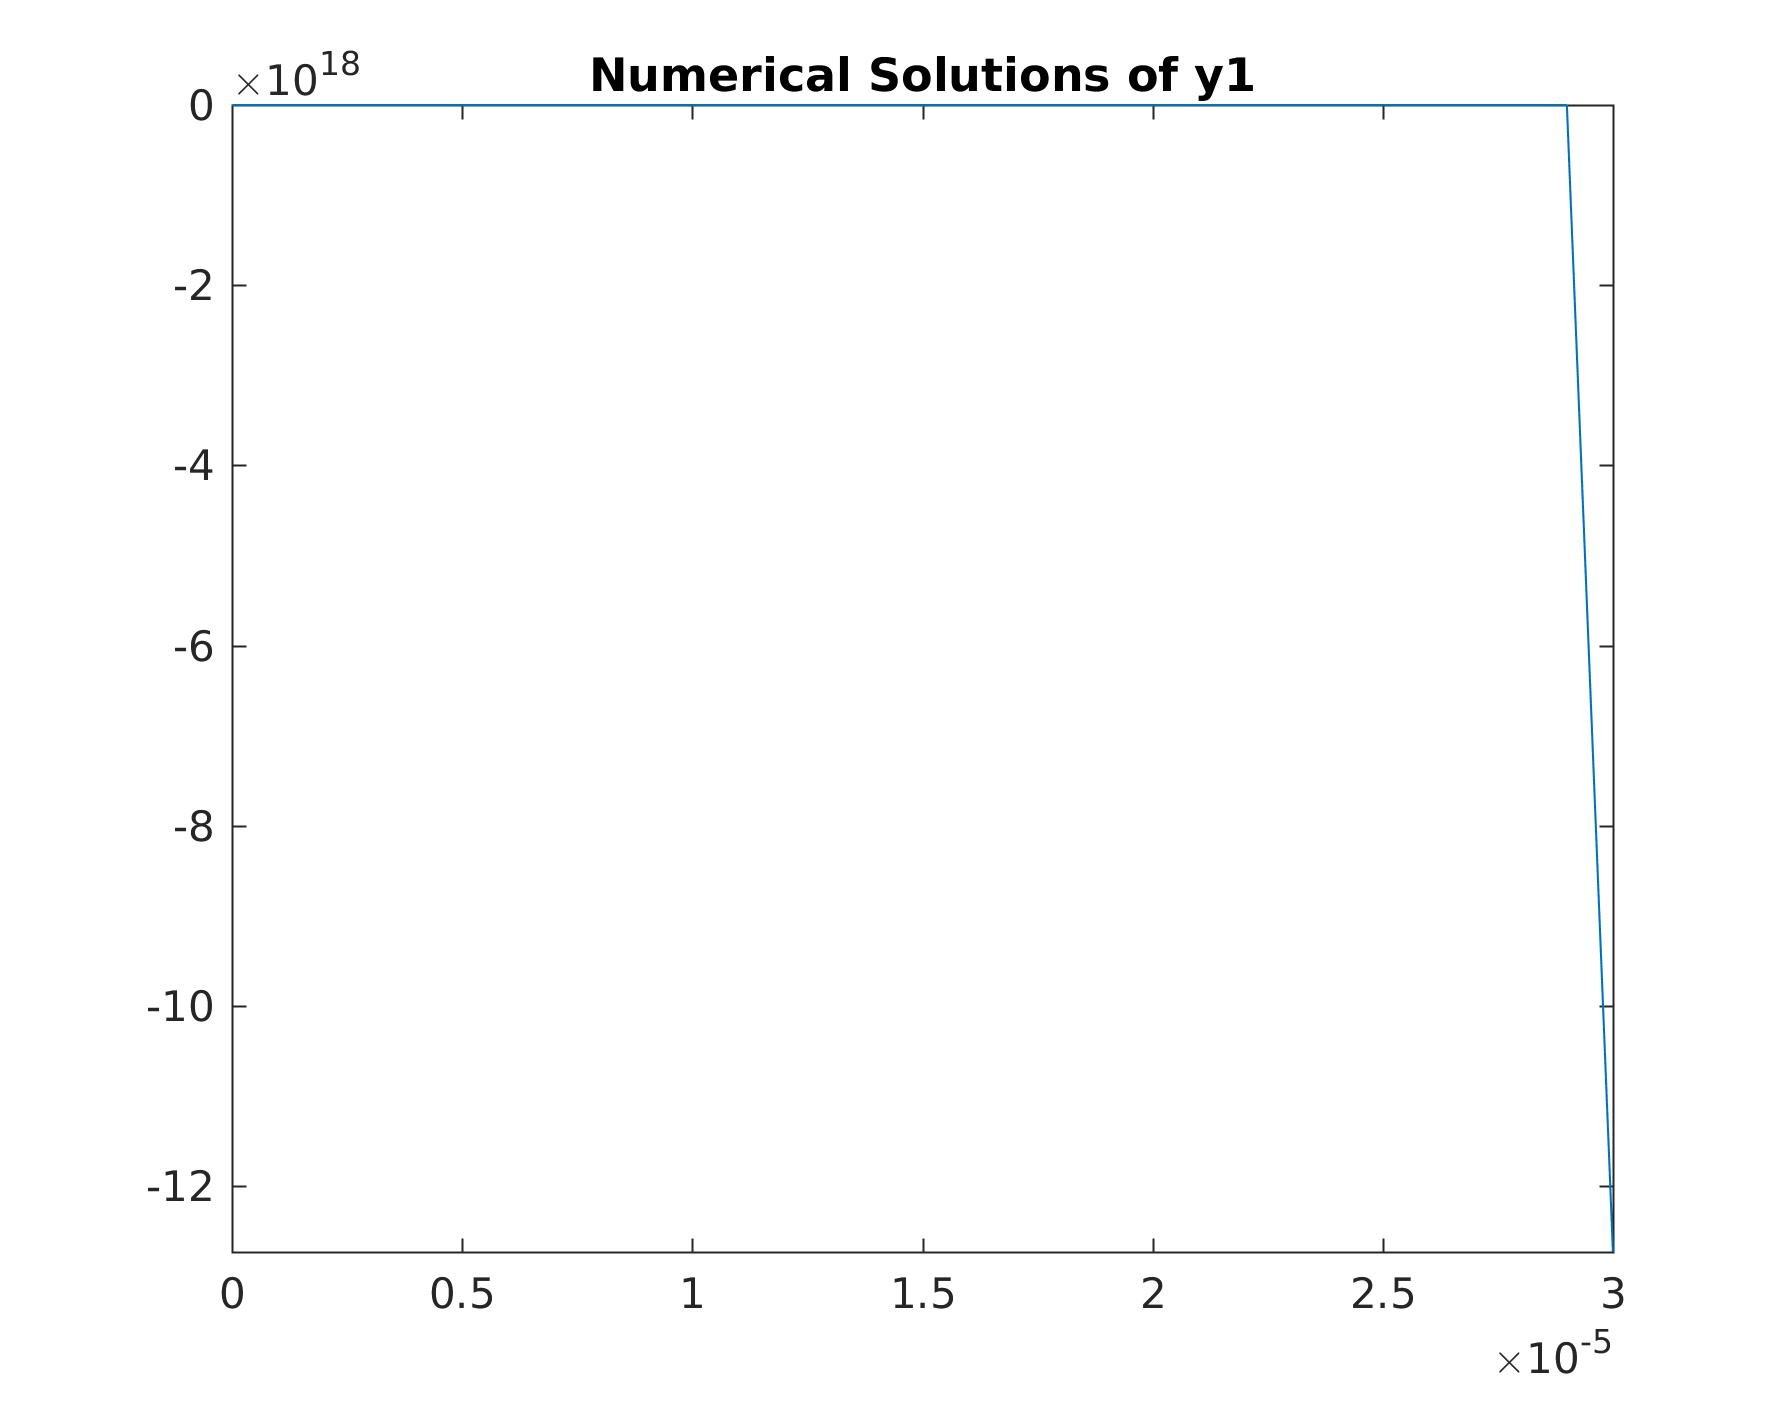
\includegraphics[scale=0.18]{fts_vdp_y1_1e-6_nl}
\caption{\textsc{Fixed Time Step 1e-6 for van der Pol $y_1$.}}
\end{figure}
\begin{figure}[H]
\centering 
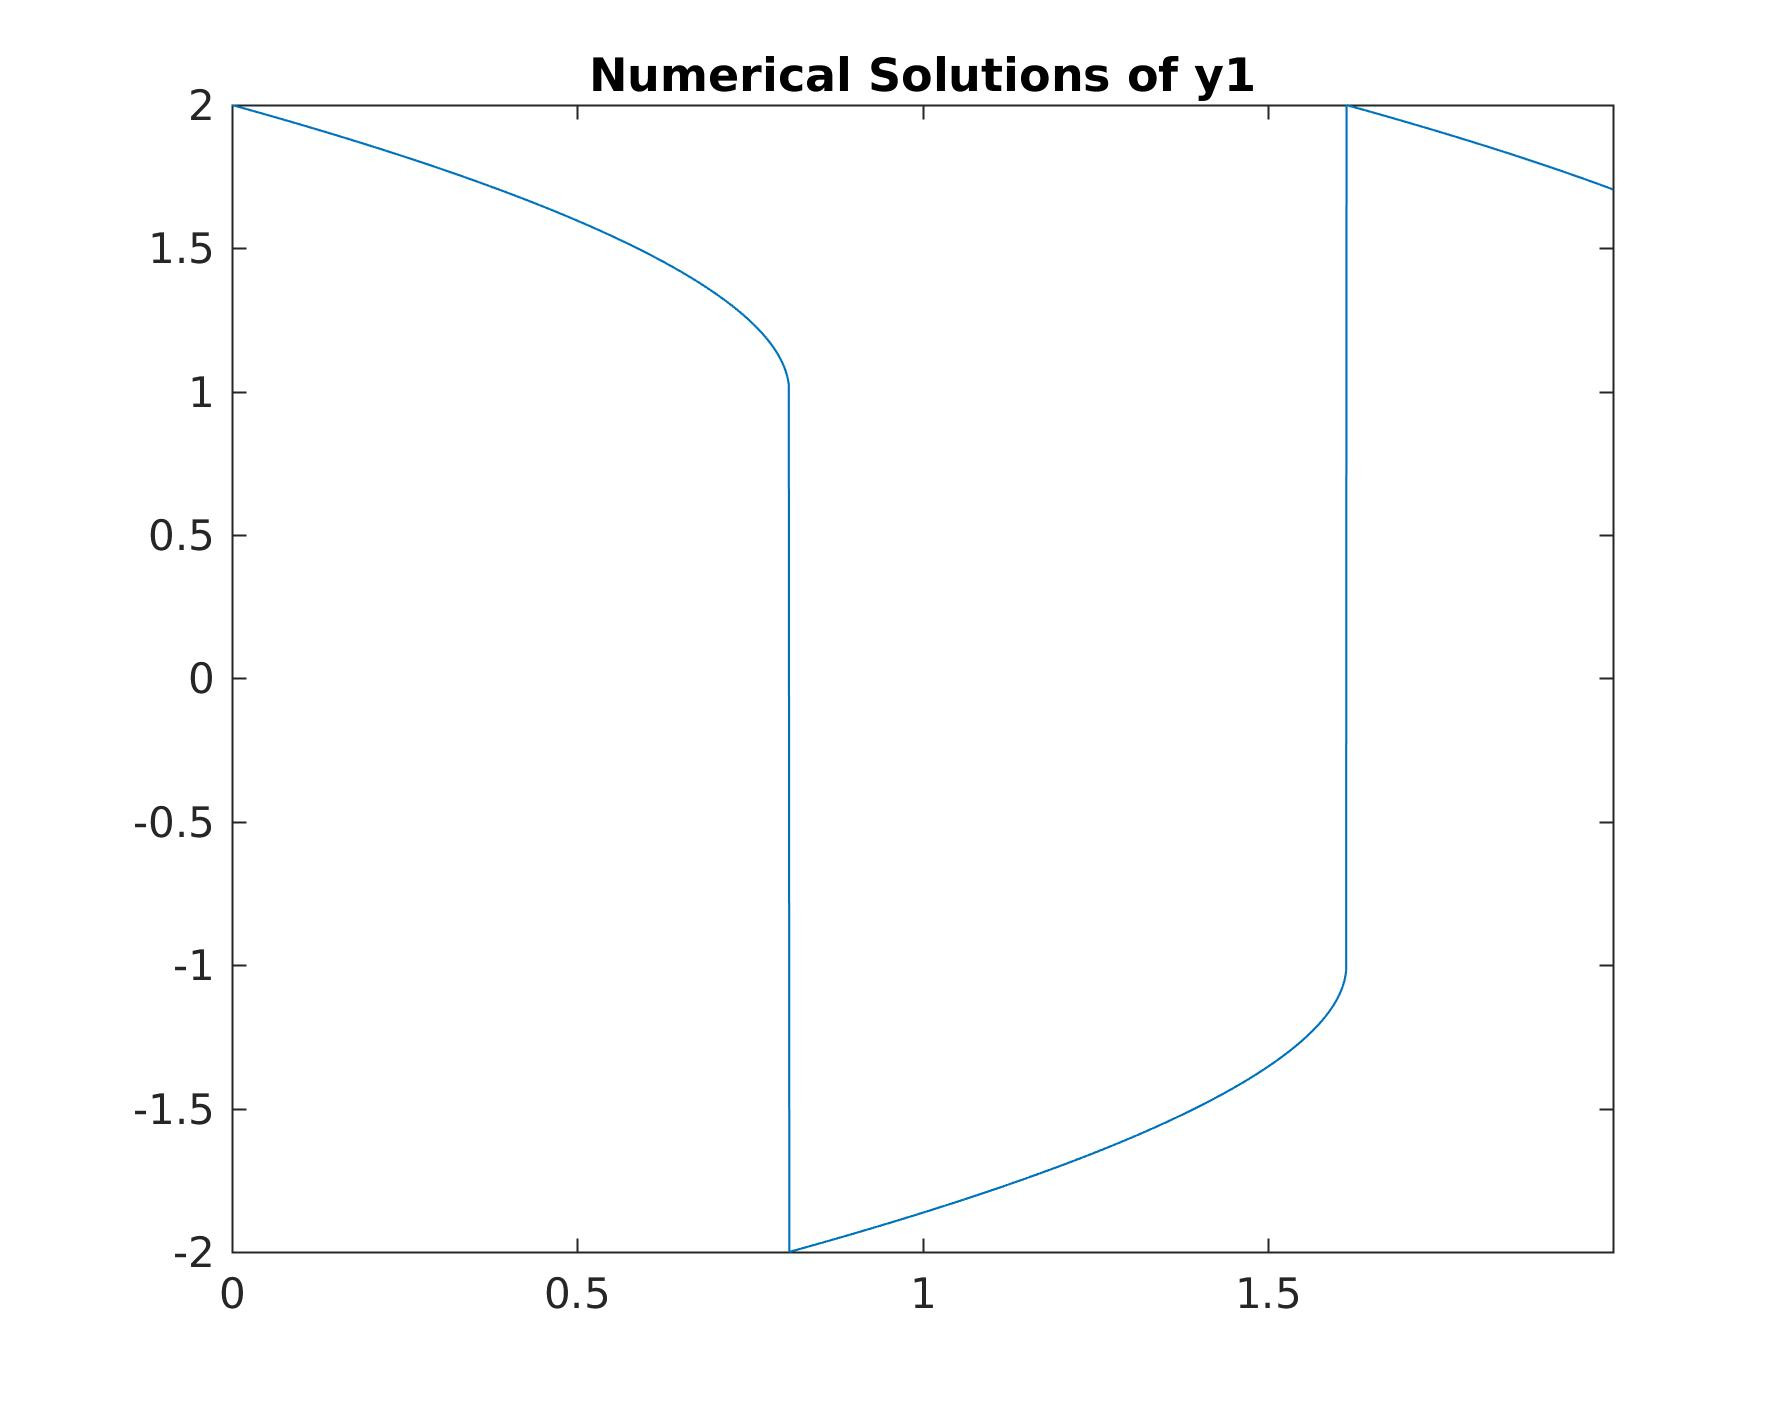
\includegraphics[scale=0.18]{fts_vdp_y1_1e-7_nl}
\caption{\textsc{Fixed Time Step 1e-7 for van der Pol $y_1$.}}
\end{figure}
\begin{figure}[H]
\centering 
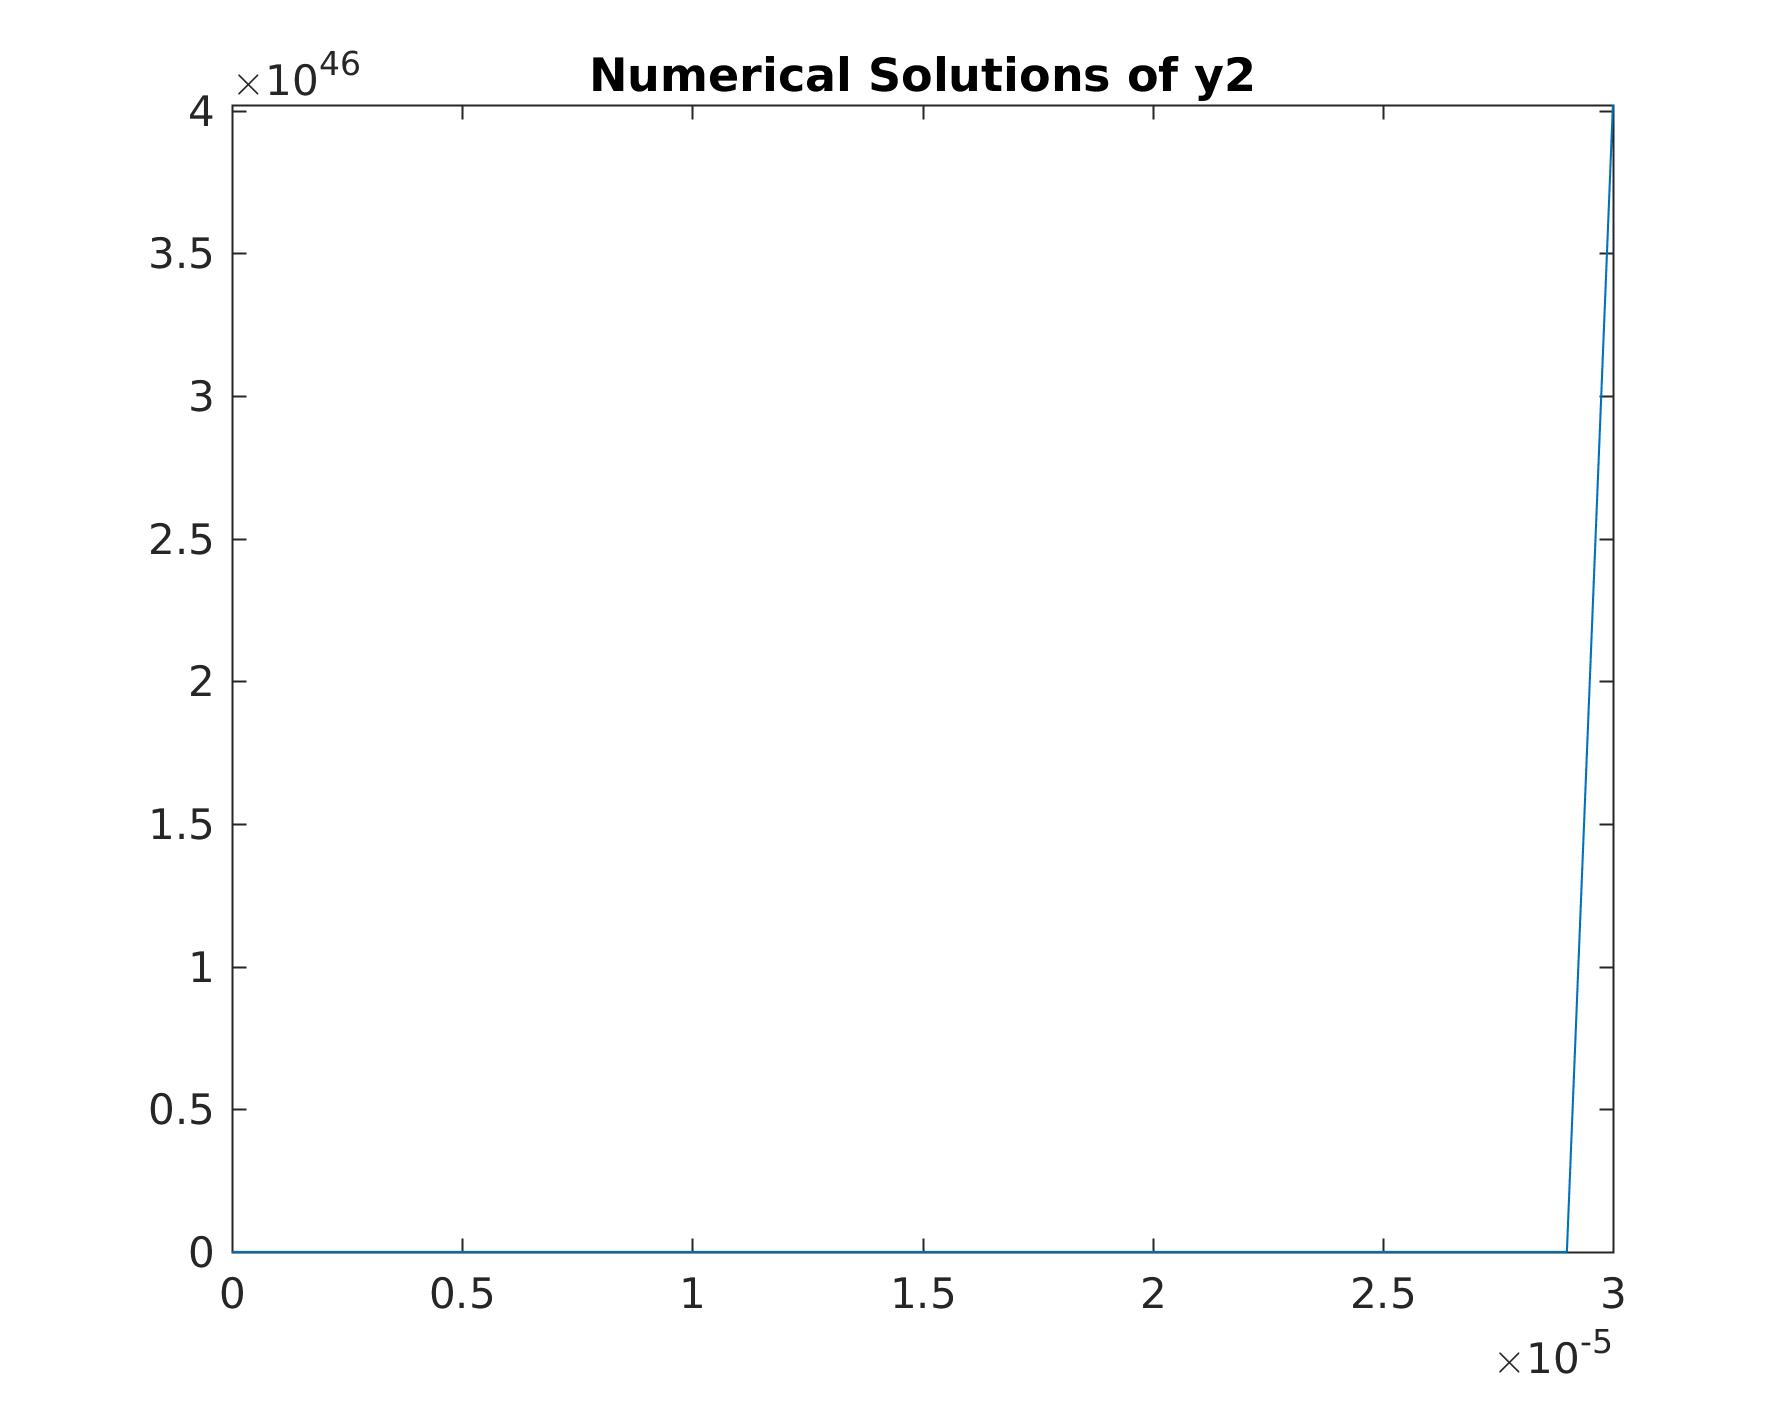
\includegraphics[scale=0.18]{fts_vdp_y2_1e-6_nl}
\caption{\textsc{Fixed Time Step 1e-6 for van der Pol $y_2$.}}
\end{figure}
\begin{figure}[H]
\centering 
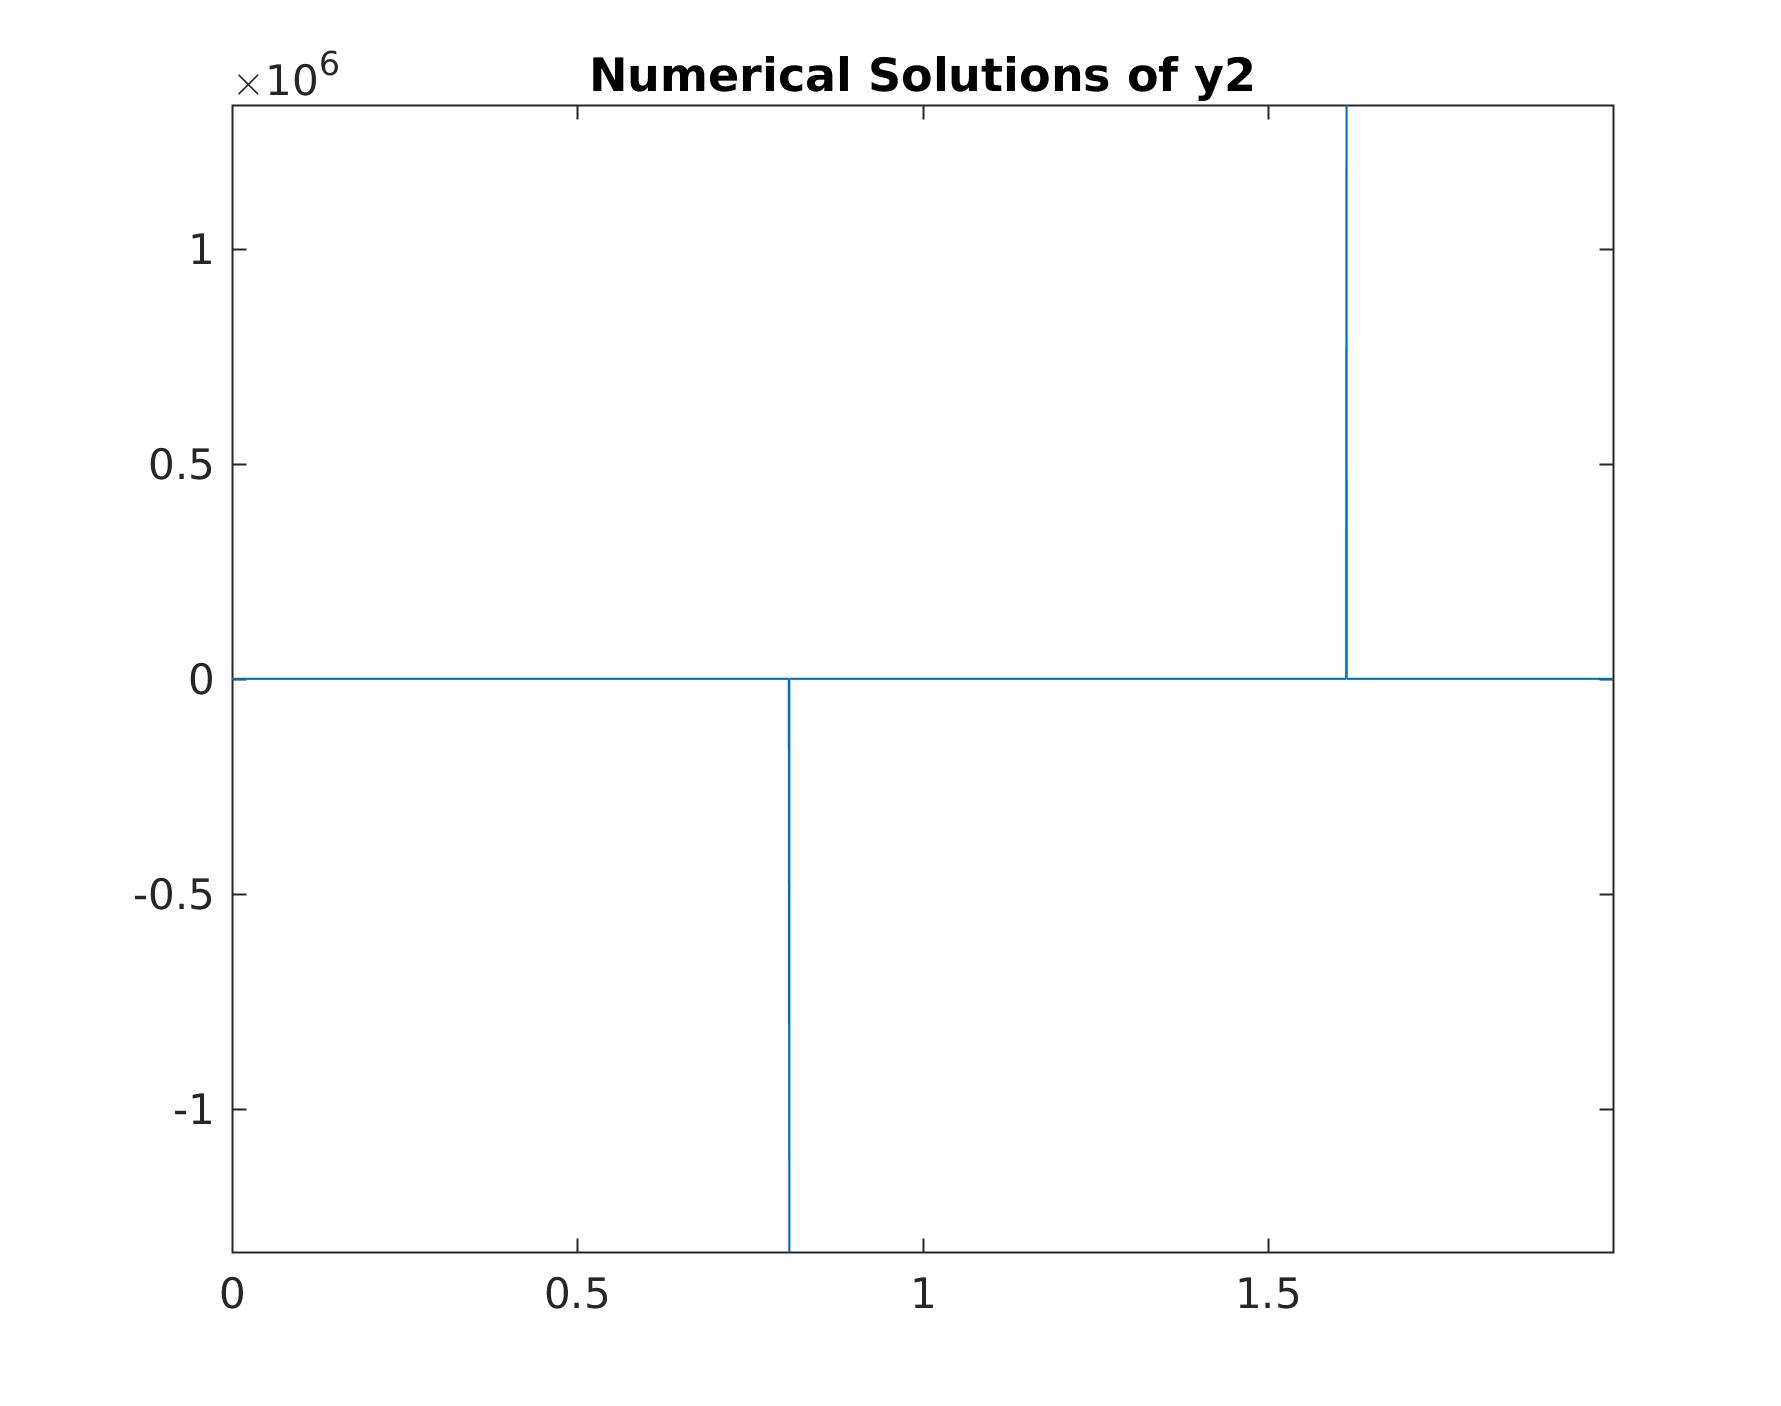
\includegraphics[scale=0.18]{fts_vdp_y2_1e-7_nl}
\caption{\textsc{Fixed Time Step 1e-7 for van der Pol $y_2$.}}
\end{figure}
Although the numerical solution with step size 1e-7  appeared to be consistent with the correct solution we found on the internet, it took considerable time to compute and memory to store the result.

Since this is only a simple equation, we can image that the equations we encounters in real life are much more complex and the computational cost using this method would be prohibitive.

In this article, we are going to introduce one way to overcome this problem: The Runge Kutta method with adaptive time step.


\section{Implementations}
We have implement adaptive time steps algorithm by both \textsc{Matlab} and \textsc{Fortran} codes. See the scripts attached to this context and the results of these scripts in the next chapter. An illustration for the fact that time steps changed amazingly in adaptive time step algorithm is represented in the following figure.
\begin{figure}[H]
\centering
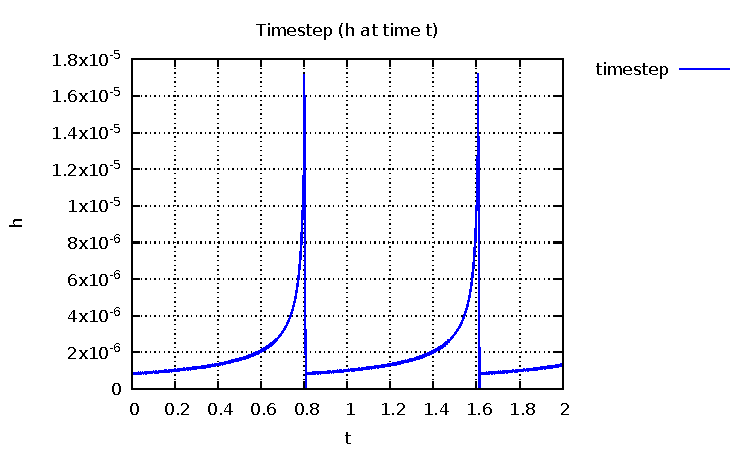
\includegraphics[scale=1.1]{vdp_ts}
\caption{\textsc{Time Step of Adaptive Time Steps for vand der Pol equation.}}
\end{figure}
\noindent
\textbf{Remark 7.1.} Observe the above figure, we see that time step size will decrease rapidly at stiff places.

\chapter{Implementations}
This chapter aims to implement some popular mathematical models, which are listed in the very beginning of this context, by using both \textsc{Matlab} and \textsc{Fortran} codes. Reader should go to Appendices A and B to see the very detailed user guides, written by the second author, on both Ubuntu 16.04 LTS and Windows 10 platform.
\section{Curtiss-Hirschfelder Equation}
In this subsection, we will use explicit Runge Kutta fourth order method\index{explicit Runge Kutta fourth order method} to solve the Curtiss-Hirschfelder equation numerically.\\
\\
\textbf{Definition 4.1.} The Curtiss-Hirschfelder equation\index{Curtiss-Hirschfelder equation} is an ordinary differential equation\index{ordinary differential equation} (ODE) which has the following form
\begin{align}
\label{4.164}
\dfrac{{dy}}{{dt}} &=  - 50\left( {y - \cos t} \right)\\
y\left( 0 \right) &= 1
\end{align}
In general, 
\begin{align}
\dfrac{{dy}}{{dt}} &= f\left( {t,y} \right)\\
y\left( {{x_0}} \right) &= {y_0}
\end{align}
\textsc{Applications.} Used to test numerical methods for the solution of ODEs.
\subsection{\textsc{Matlab} Codes}
The following \textsc{Matlab} routines aims at
\begin{enumerate}
\item Approximating solution of \eqref{4.164} by using explicit Runge Kutta fourth order method.
\item Compute absolute errors\index{absolute errors} and relative errors\index{relative errors} and plot the obtained numerical solutions and errors.
\end{enumerate}
\subsubsection{Subroutine s.m}
This subroutine provides the exact solution of \eqref{4.164}.
\begin{verbatim}
function s = s(t)

s = 50/2501*(50*cos(t)+sin(t)) + exp(-50*t)/2501;
\end{verbatim}
\subsubsection{Subroutine f.m}
This subroutine provides the function $f$ in right-hand side of \eqref{4.164}. Users can modify these functions later.
\begin{verbatim}
function f = f(t,y)

f = -50*y + 50*cos(t);
\end{verbatim}
\subsubsection{Subroutine x.m}
This subroutine provides the explicit Runge Kutta fourth order method.
\begin{verbatim}
function x = x(a,b,c,h,t,y)

k1 = f(t,y);
k2 = f(t+c(2)*h,y+h*a(2,1)*k1);
k3 = f(t+c(3)*h,y+h*(a(3,1)*k1+a(3,2)*k2));
k4 = f(t+c(4)*h,y+h*(a(4,1)*k1+a(4,2)*k2+a(4,3)*k3));
x  = h*(b(1)*k1+b(2)*k2+b(3)*k3+b(4)*k4);
\end{verbatim}
\subsubsection{Main Routine RK4}
\begin{verbatim}
close all
clear all
clc
format long

tic

%% Initial.

A1(1) = 1;
A2(1) = 1;
% A3(1) = 1;

N=1000;
h=25/N;
t = 0:h:25;

%% Coefficients

a1 = [0 0 0 0 ;
    1/2 0 0 0 ;
    0 1/2 0 0 ;
    0 0 1 0];
b1 = [1/6 1/3 1/3 1/6];
c1 = [0 1/2 1/2 1];

a2 = [0 0 0 0 ;
    1/3 0 0 0 ;
    -1/3 1 0 0 ;
    1 -1 1 0];
b2 = [1/8 3/8 3/8 1/8];
c2 = [0 1/3 2/3 1];

%% Numerical Solution.

for n=1:N
    A1(n+1) = A1(n) + x(a1,b1,c1,h,t(n),A1(n));
    A2(n+1) = A2(n) + x(a2,b2,c2,h,t(n),A2(n));
end

%% Plot Numerical Solution 

figure(1)
hold on
plot(t,s(t),'b');
plot(t,A1,'r');
legend('Exact Solution','Numerical Solution');
title('Numerical Solution (Butcher Table 1)');

figure(2)
hold on
plot(t,s(t),'b');
plot(t,A2,'r');
legend('Exact Solution','Numerical Solution');
title('Numerical Solution (Butcher Table 2)');

%% Absolute Error.

display('Absolute Error 1')
ae1 = h*sum(abs(A1-s(t)))

display('Absolute Error 2')
ae2 = h*sum(abs(A2-s(t)))

figure(3)
hold on
plot(t,abs(A1-s(t)),'g');
plot(t,abs(A2-s(t)),'b');
legend('a1 b1 c1','a2 b2 c2');
title('Absolute Error');

%% Relative Error.

display('Relative Error 1')
re1 = h*sum(abs((A1-s(t))./s(t)))
display('Relative Error 2')
re2 = h*sum(abs((A2-s(t))./s(t)))

figure(4)
hold on
plot(t,abs((A1-s(t))./A1),'g');
plot(t,abs((A2-s(t))./A2),'b');
legend('a1 b1 c1','a2 b2 c2');
title('Relative Error');
toc
\end{verbatim}
\subsection{Results}
\begin{figure}[H]
\centering
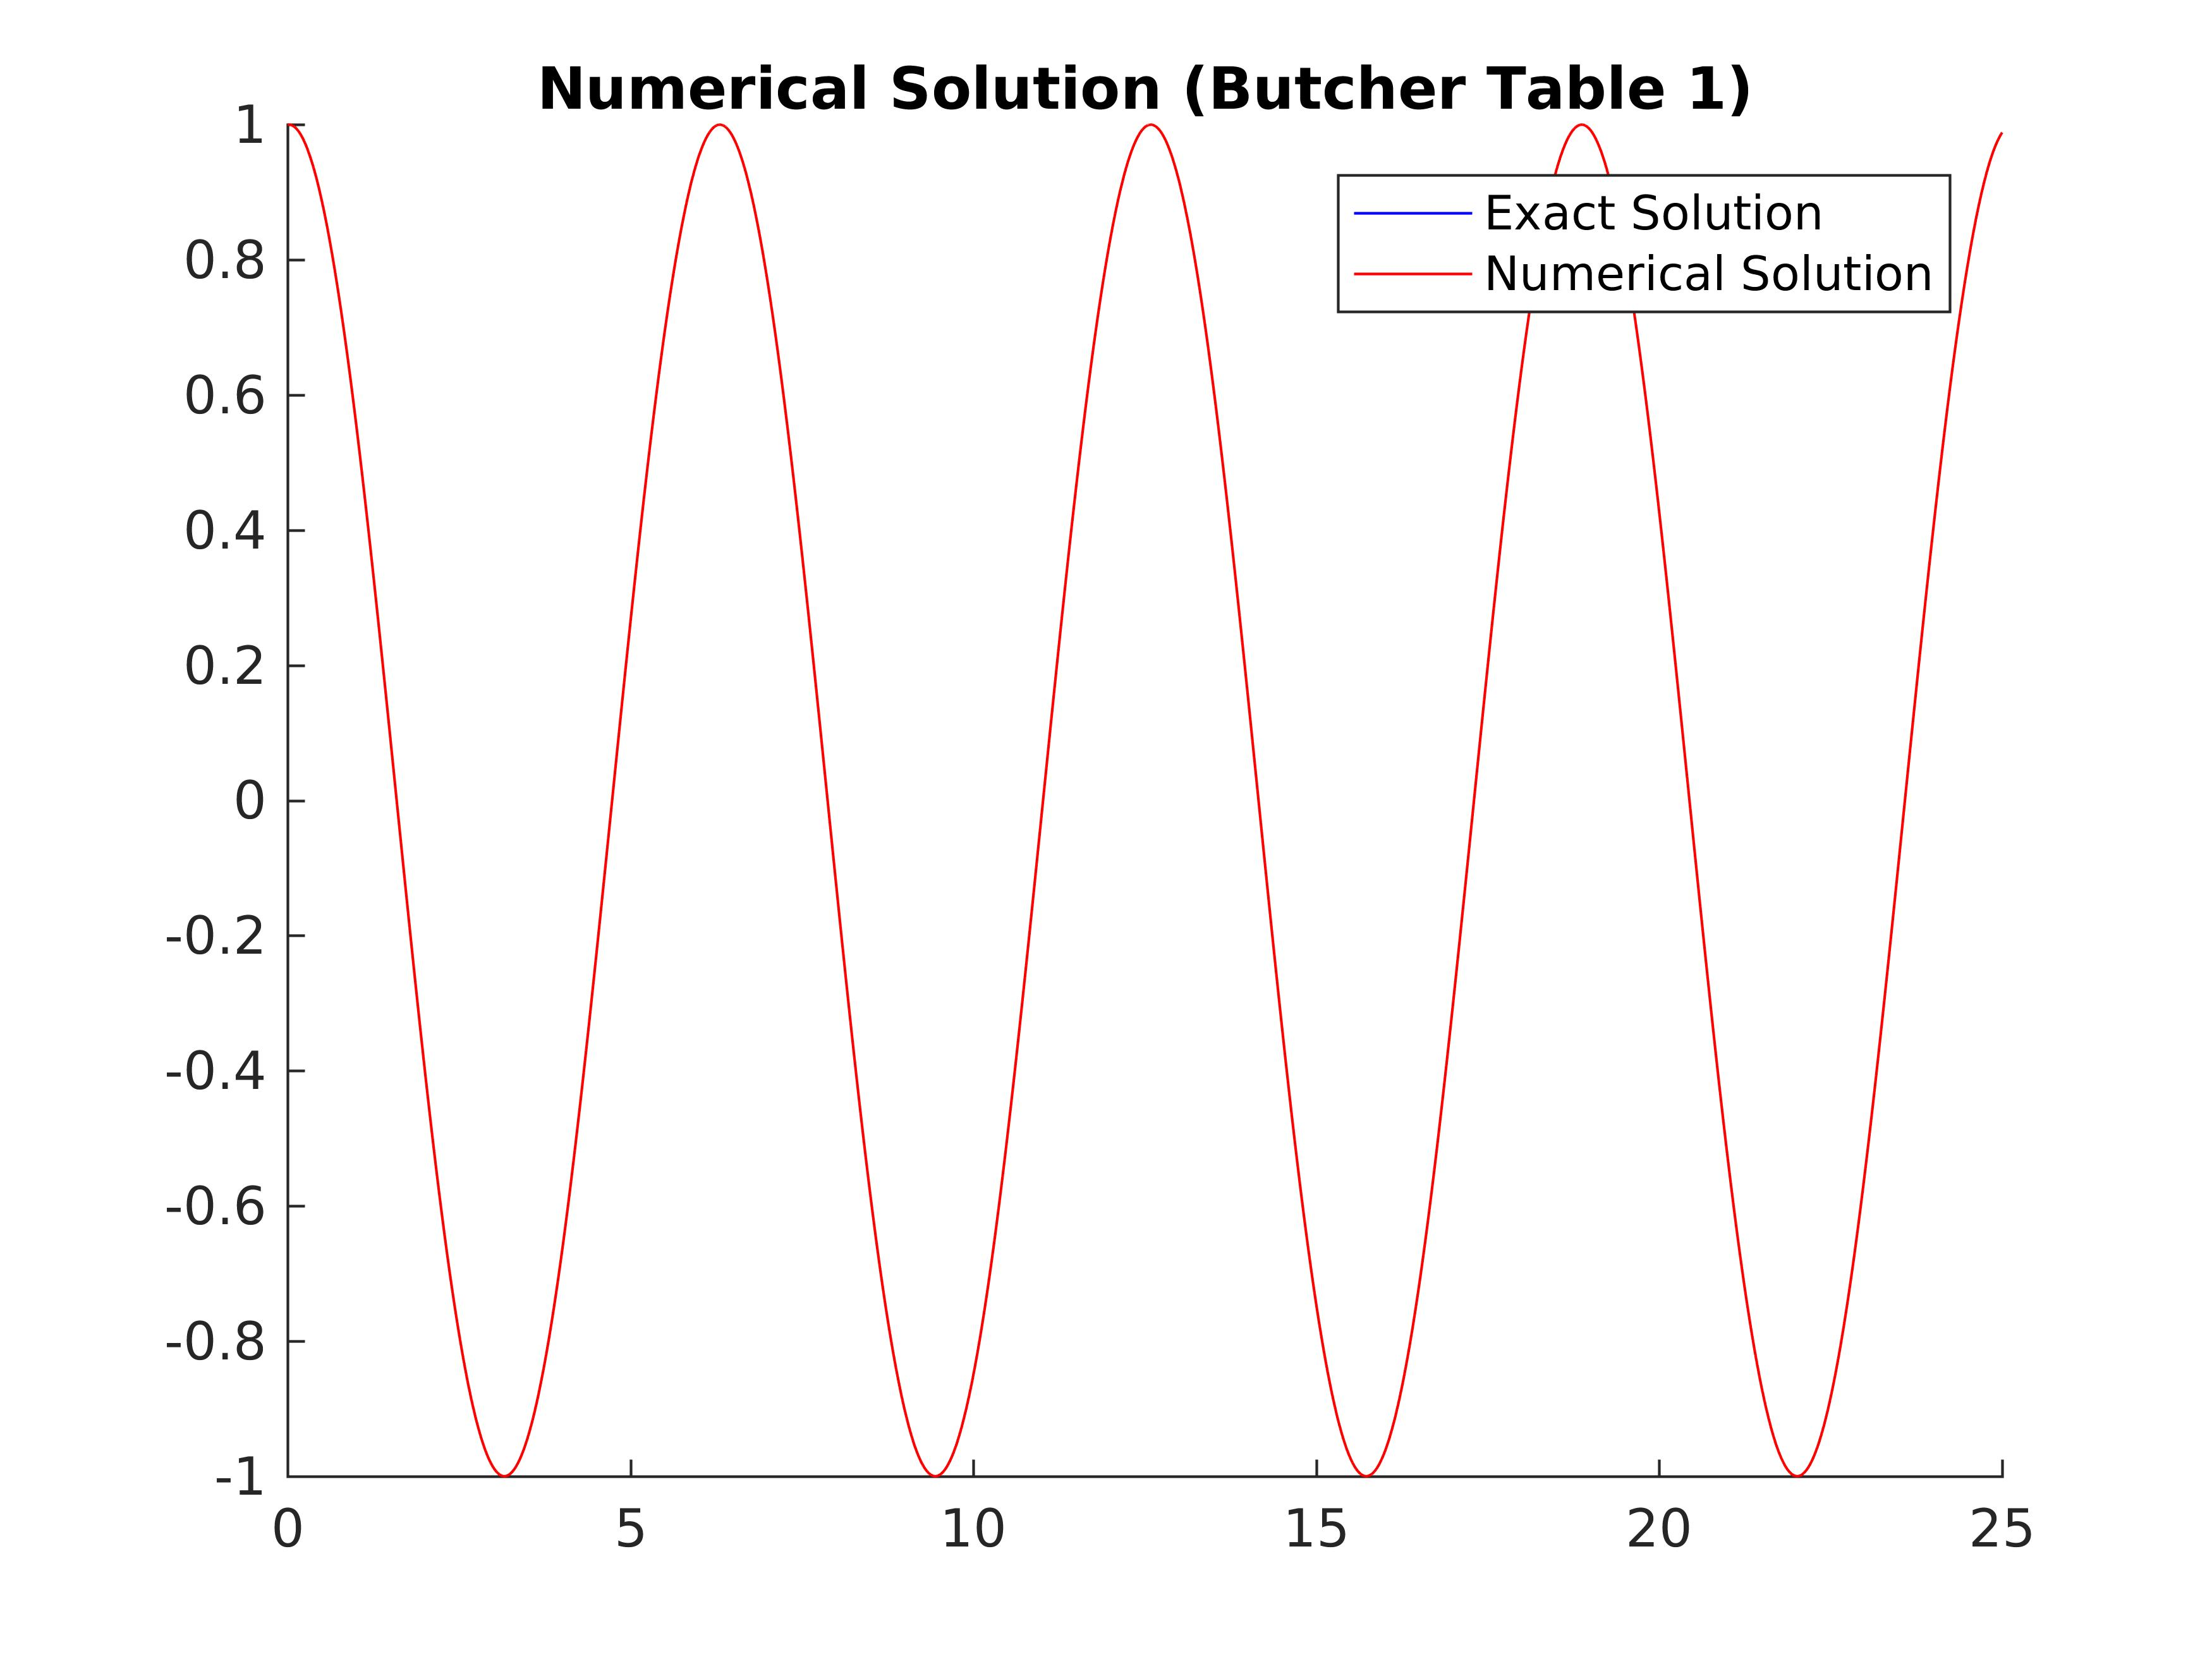
\includegraphics[scale=0.09]{ns1}
\caption{\textsc{Numerical Solutions for Curtiss-Hirschfelder equation by Matlab.}}
\end{figure}
\begin{figure}[H]
\centering
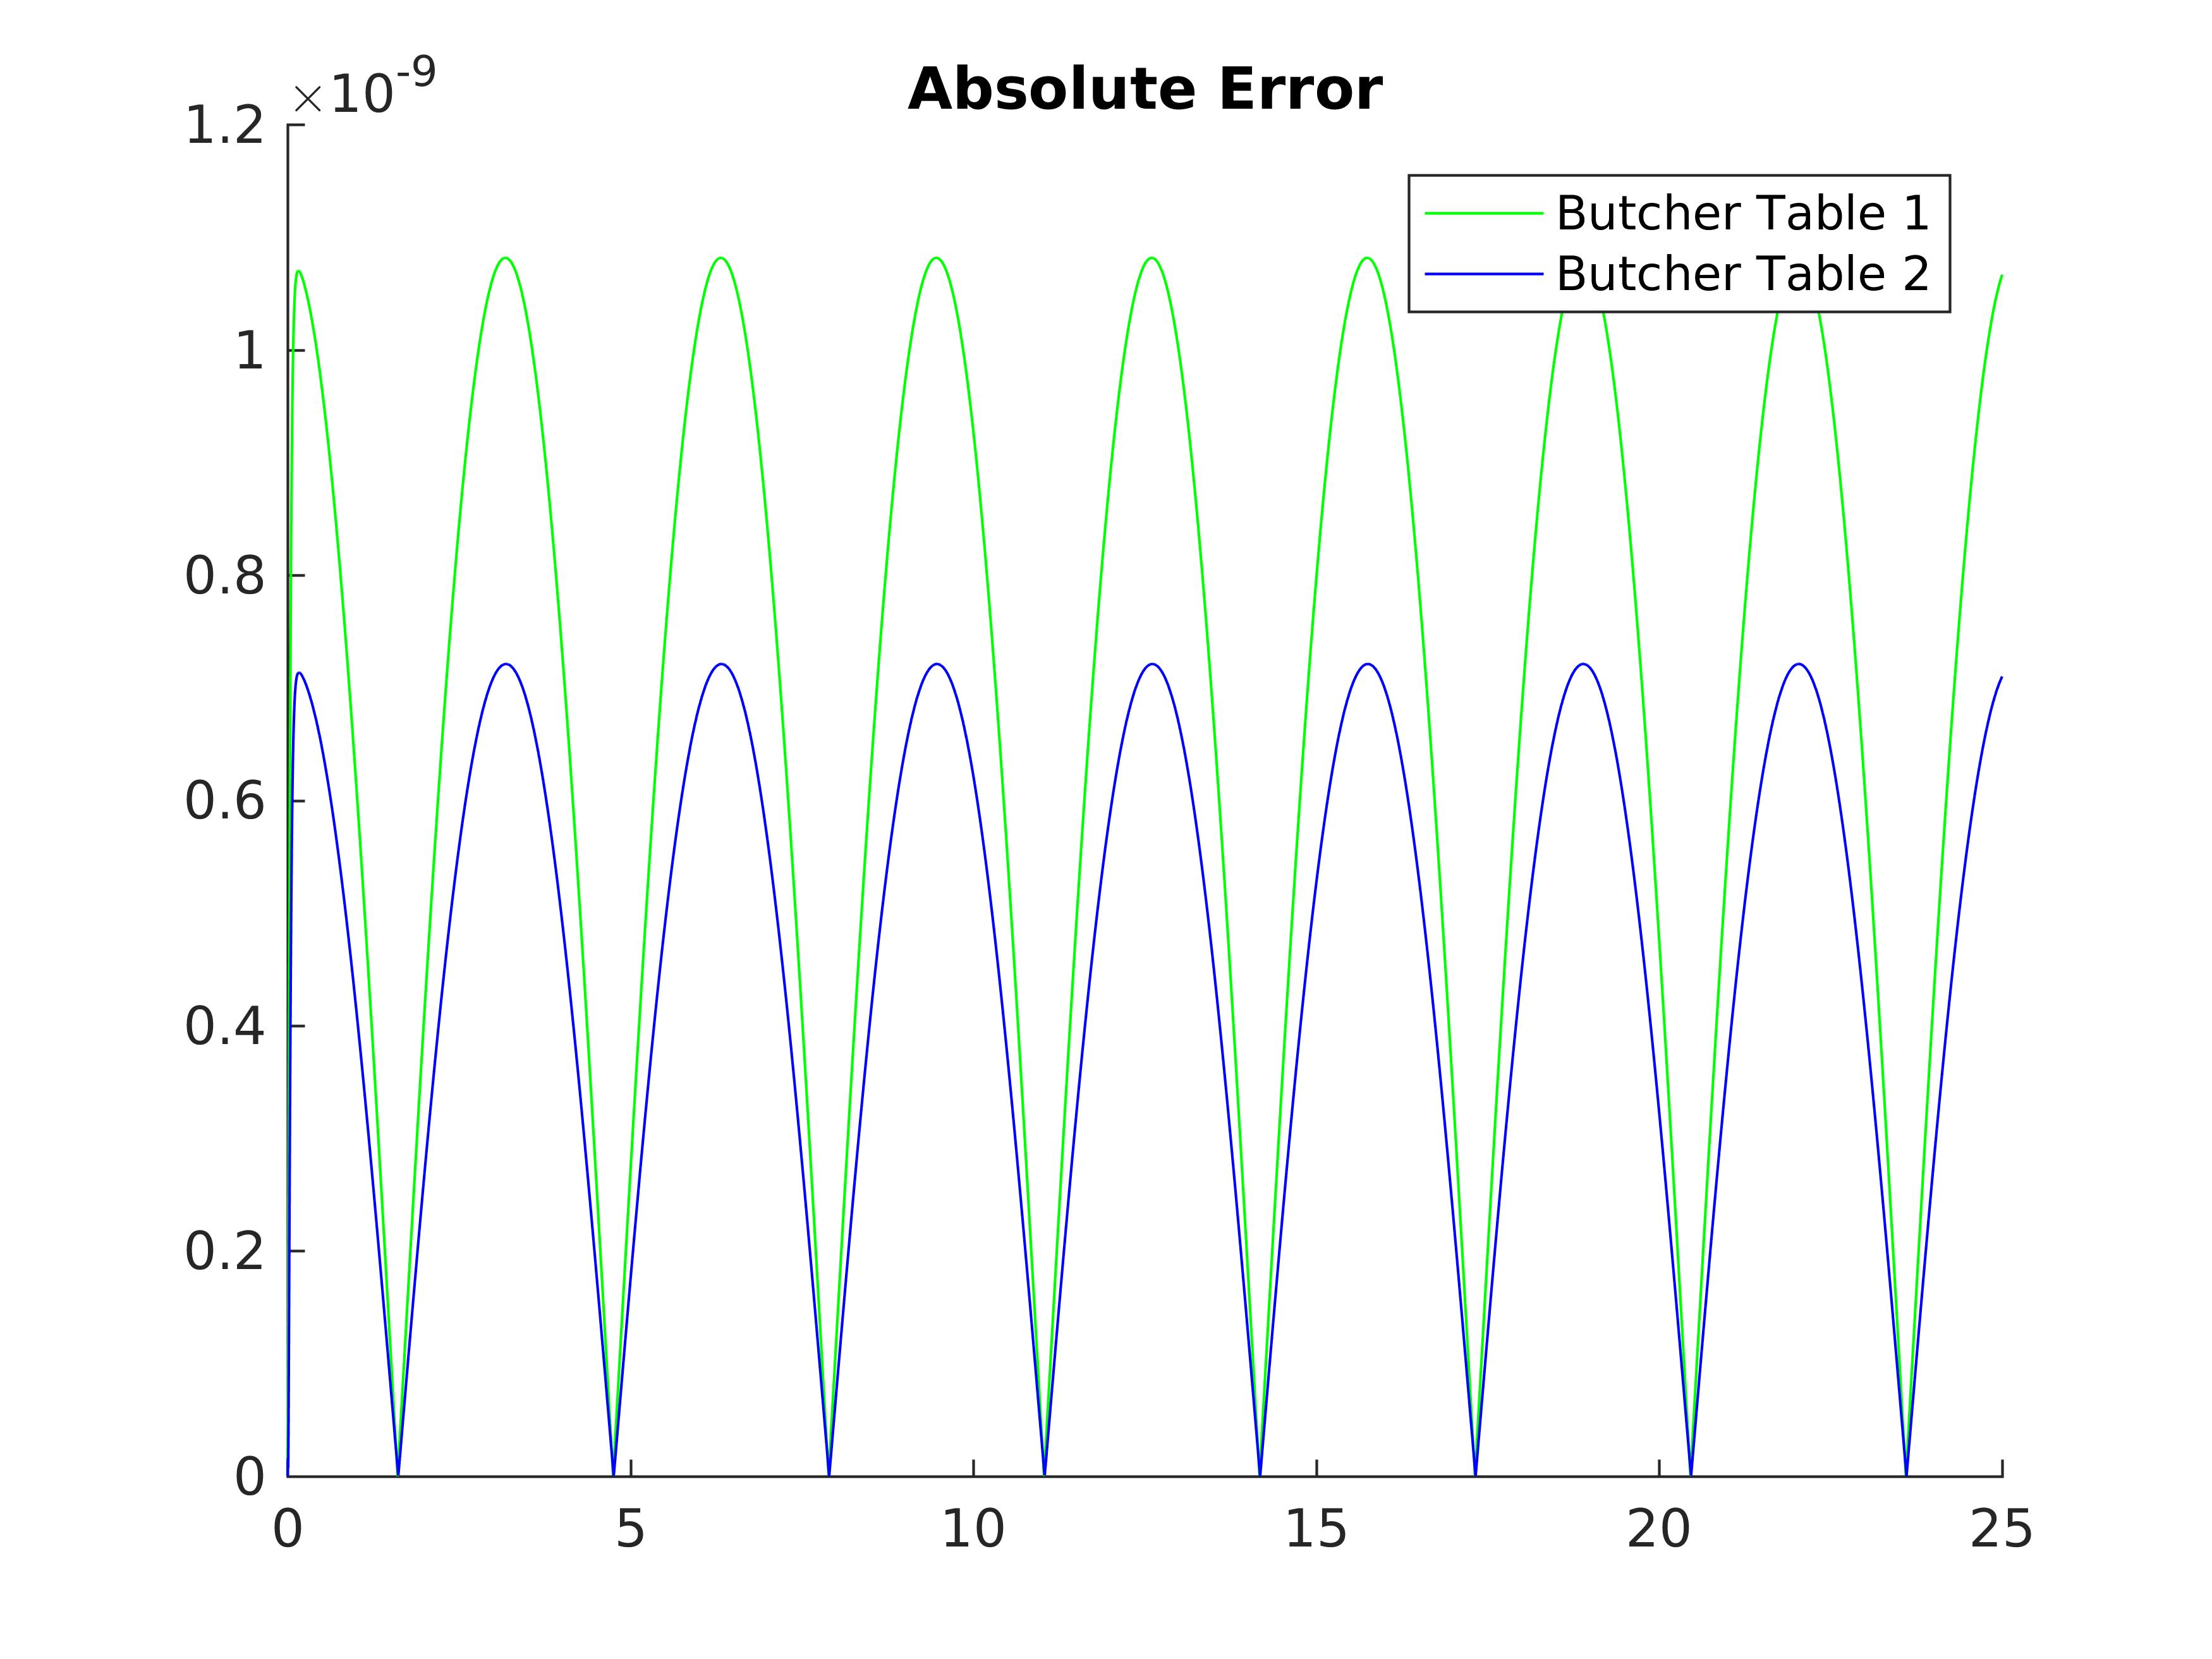
\includegraphics[scale=0.09]{ae}
\caption{\textsc{Absolute Errors for Curtiss-Hirschfelder equation by Matlab.}}
\end{figure}
\begin{figure}[H]
\centering
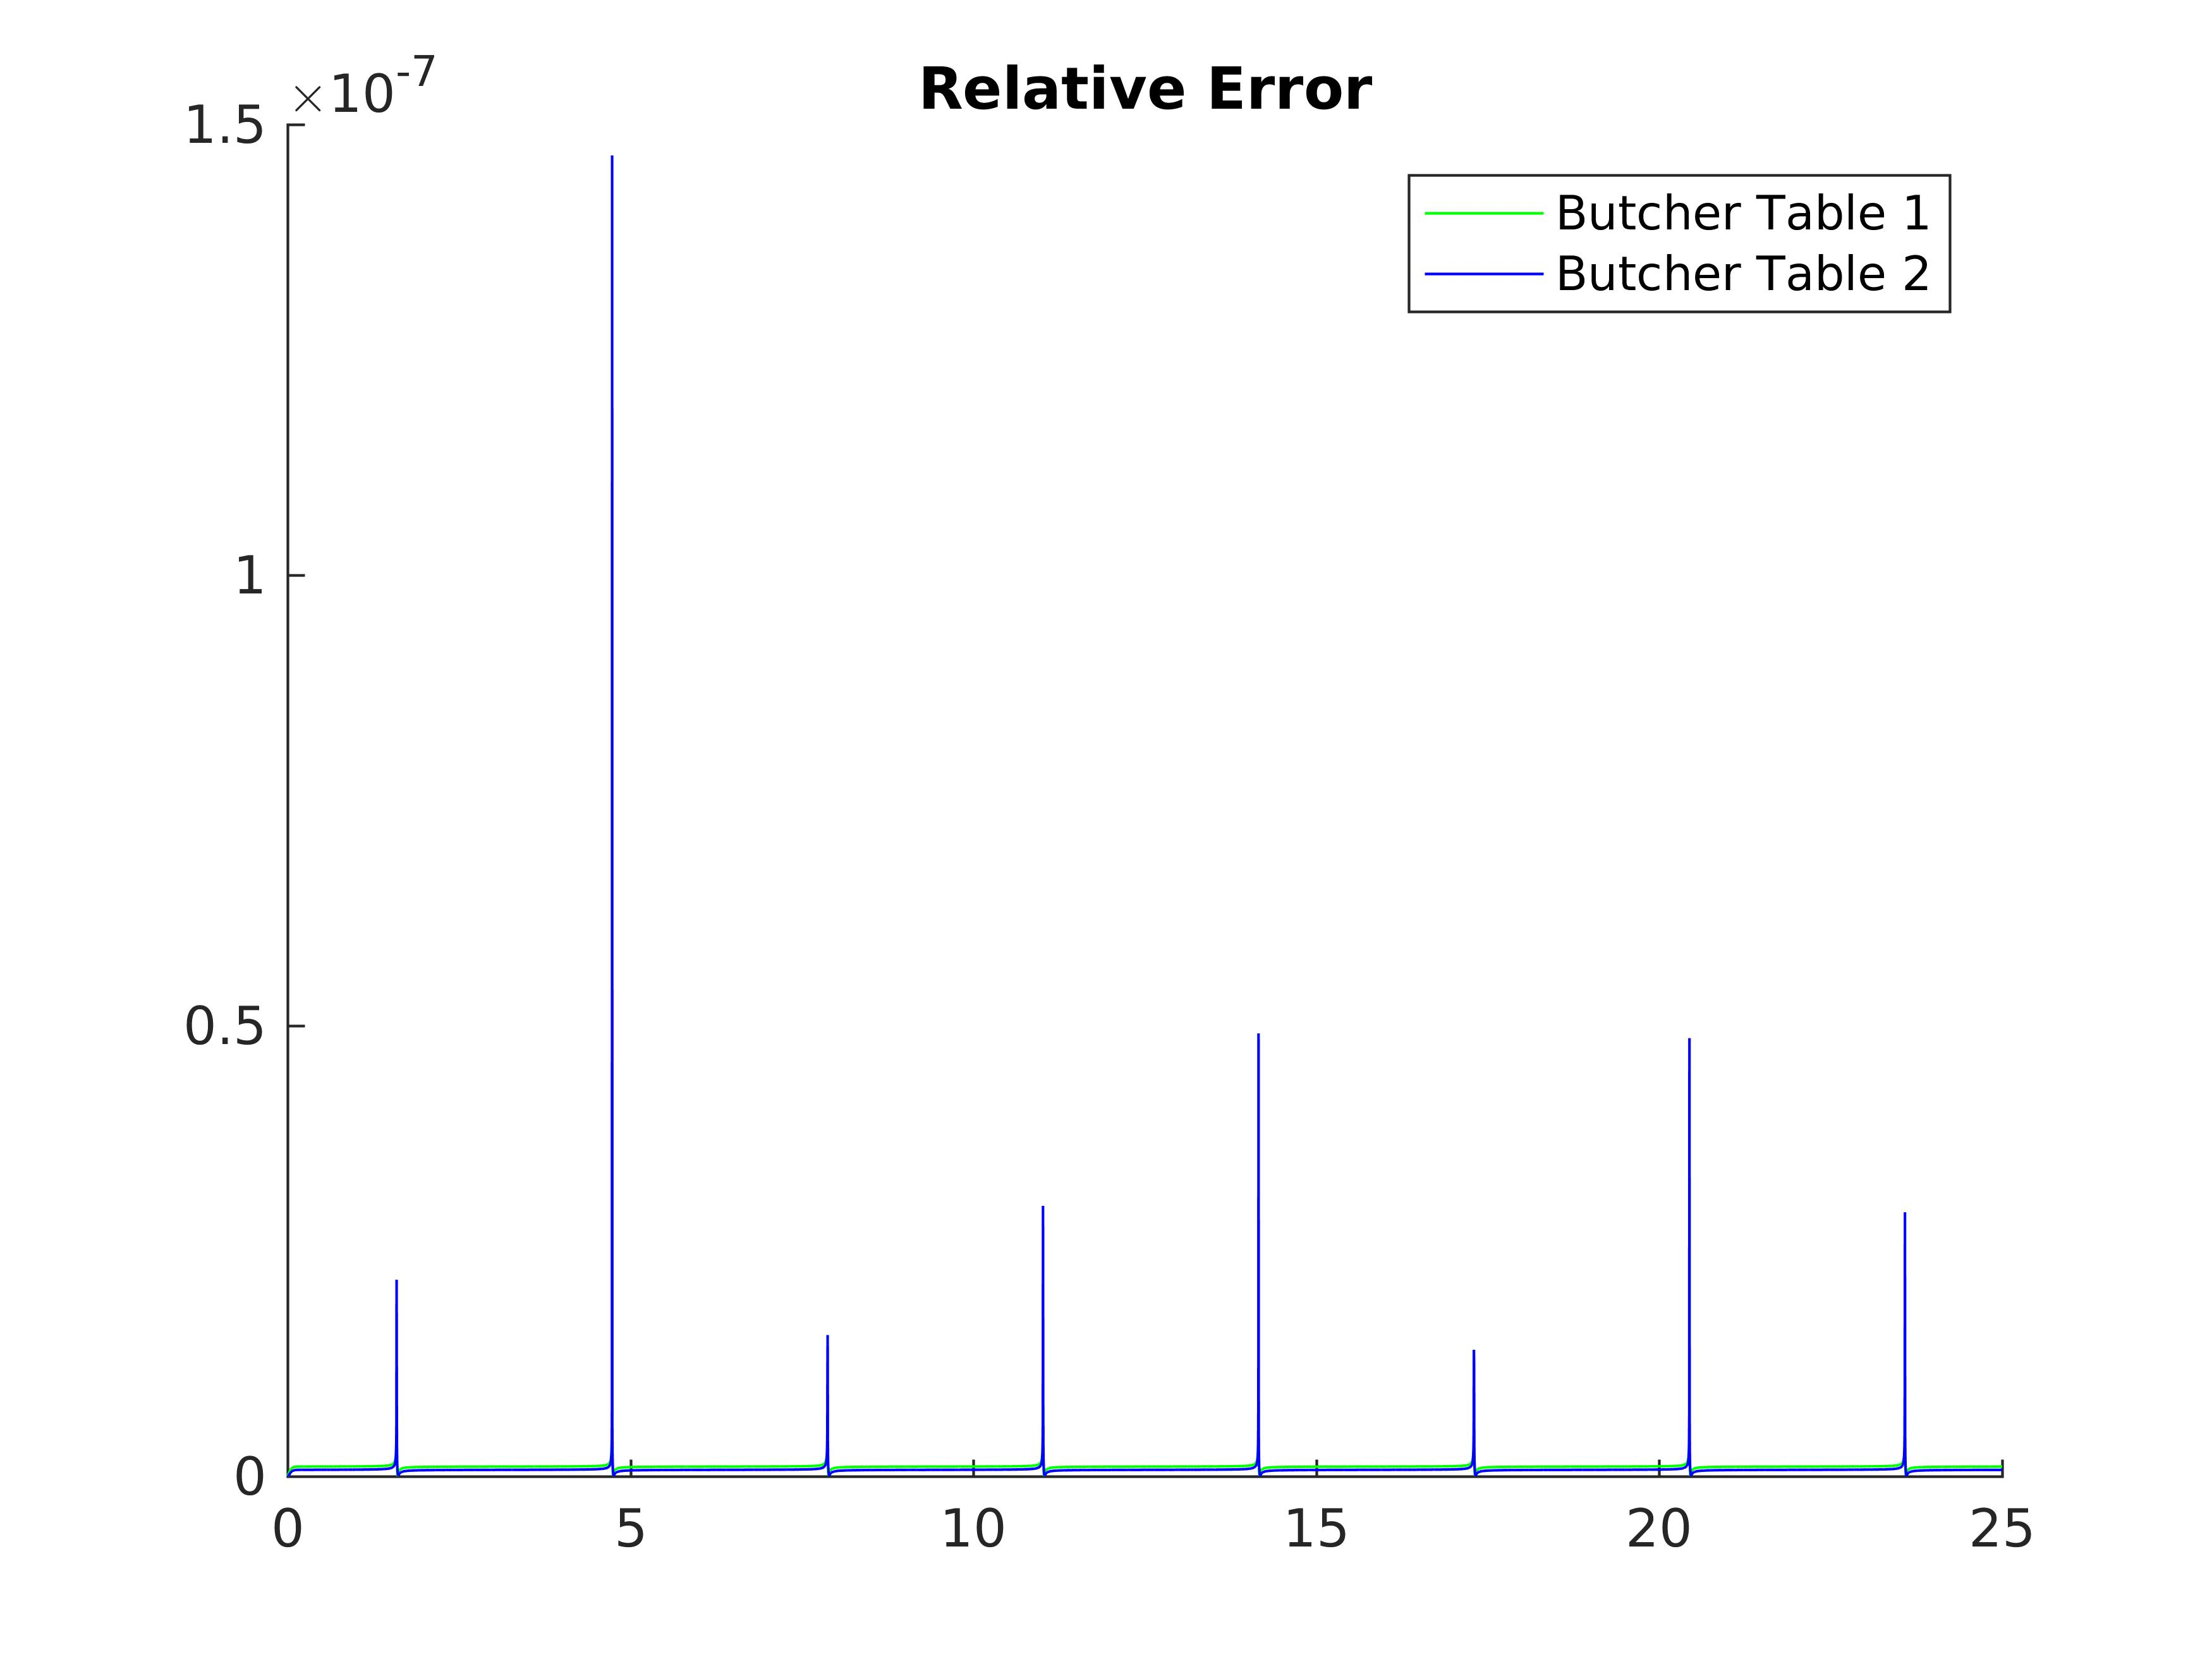
\includegraphics[scale=0.09]{re}
\caption{\textsc{Relative Errors for Curtiss-Hirschfelder equation by Matlab.}}
\end{figure}
\subsection{\textsc{Fortran} Codes}
\subsubsection{ch.f90}
\begin{lstlisting}
module ch  
implicit none 
	integer, parameter :: dms=1 ! number of unknowns
    ! initial condition
	real (kind = 8), dimension(dms) :: x=(/1d0/) 
    ! beginning and ending time points
	real (kind = 8) :: t=0d0,te=40d0 
	real (kind = 8) :: d=real(dms)
contains      
	subroutine f(t,y,f0)
		implicit none
		real (kind = 8), intent(in) :: t
		real (kind = 8), dimension(dms), intent(in) :: y
		real (kind = 8), dimension(dms), intent(out) :: f0
		
		f0(1)=-50*(y(1)-cos(t))
	end subroutine f
end module ch 
\end{lstlisting}
\subsubsection{GNU Plot Results}
\begin{figure}[H]
\centering
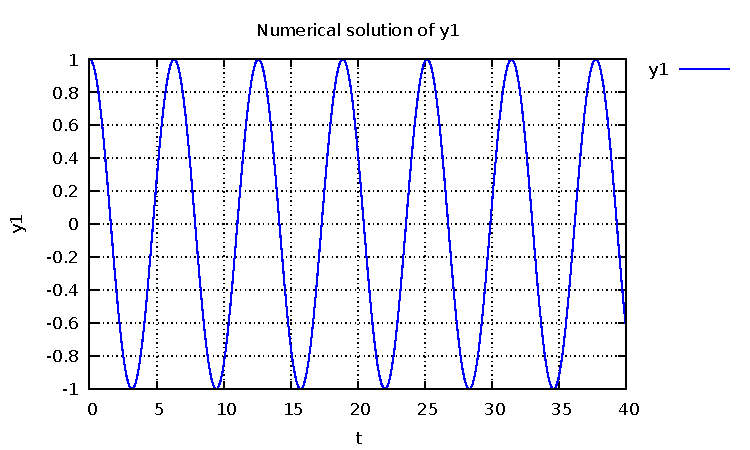
\includegraphics[scale=1.15]{ch_1}
\caption{\textsc{Numerical Solution of Curtiss-Hirschfelder equation by GNU Plot.}}
\end{figure}
\begin{figure}[H]
\centering
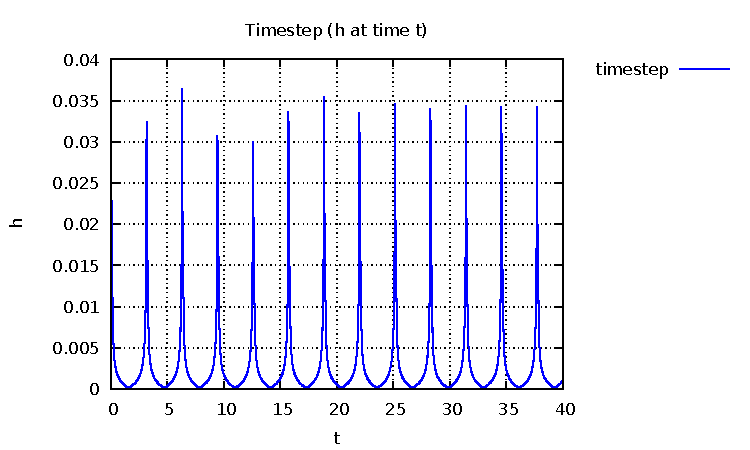
\includegraphics[scale=1.15]{ch_ts}
\caption{\textsc{Timestep of Curtiss-Hirschfelder equation by GNU Plot.}}
\end{figure}
\section{Brusselator Equation}
\textsc{Brusselator.} \index{Brusselator}
\begin{align}
    \dfrac{dy_1}{dt}  &=  1 - 4y_1 + y_1^2 y_2
    \\
    \dfrac{dy_2}{dt}  &=  3y_1 - y_1^2 y_2
\end{align}
where $y_1\left(0\right) = 1.5$ and $y_2\left(0\right) = 3$.

In general,
\begin{align}
\dfrac{{d{y_1}}}{{dt}} &= {f_1}\left( {t,{y_1},{y_2}} \right)\label{4.170}\\
\dfrac{{d{y_2}}}{{dt}} &= {f_2}\left( {t,{y_1},{y_2}} \right)\label{4.171}
\end{align}
In vector form $y=\left(y_1,y_2\right)$,
\begin{align}
\dfrac{{dy}}{{dt}} = f\left( {t,y} \right)
\end{align}
\textsc{Applications.} A theoretical model for a type of \textit{autocatalytic reaction}.
\subsection{\textsc{Matlab} Codes}
\subsubsection{Subroutine f.m}
This subroutine provides $f_1$ and $f_2$ in the right-hand side of \eqref{4.170} and \eqref{4.171}. Users can modify these functions later.
\begin{verbatim}
function f = f(t,y)

f(1) = 1-4*y(1)+y(1)^2*y(2);
f(2) = 3*y(1)-y(1)^2*y(2);
\end{verbatim}
\subsubsection{Subroutine x.m}
This subroutine provides the explicit Runge Kutta fourth order method\index{explicit Runge Kutta fourth order method}.
\begin{verbatim}
function x = x(a,b,c,h,t,y)

k1 = f(t,y);
k2 = f(t+c(2)*h,y+h*a(2,1)*k1);
k3 = f(t+c(3)*h,y+h*(a(3,1)*k1+a(3,2)*k2));
k4 = f(t+c(4)*h,y+h*(a(4,1)*k1+a(4,2)*k2+a(4,3)*k3));
x  = h*(b(1)*k1+b(2)*k2+b(3)*k3+b(4)*k4);
\end{verbatim}
\subsubsection{Main Routine RK4.m}
\index{absolute error}\index{relative error}
\begin{verbatim} 
clear all
close all
clc
format long

tic
%% Initial for Reference Solutions.
N0 = 10^6;
h0= 20/N0;
t0 = 0:h0:20;

B1 = zeros(N0,2);
B1(1,1) = 1.5;
B1(1,2) = 3;

B2 = zeros(N0,2);
B2(1,1) = 1.5;
B2(1,2) = 3;

%% Initial for Numerical Solutions.
N = 10^4;
h = 20/N;
t = 0:h:20;

A1 = zeros(N,2);
A1(1,1) = 1.5;
A1(1,2) = 3;

A2 = zeros(N,2);
A2(1,1) = 1.5;
A2(1,2) = 3;

A3 = zeros(N,2);
A3(1,1) = 1.5;
A3(1,2) = 3;

% Step 
step = N0/N;

%% Explicit Runge Kutta initials.
% Coefficients
a1 = [0 0 0 0 ;
    1/2 0 0 0 ;
    0 1/2 0 0 ;
    0 0 1 0];
b1 = [1/6 1/3 1/3 1/6];
c1 = [0 1/2 1/2 1];

a2 = [0 0 0 0 ;
    1/3 0 0 0 ;
    -1/3 1 0 0 ;
    1 -1 1 0];
b2 = [1/8 3/8 3/8 1/8];
c2 = [0 1/3 2/3 1];

%% Reference Solutions.
for n=1:N0
    B1(n+1,:) = B1(n,:) + x(a1,b1,c1,h0,t0(n),B1(n,:));
    B2(n+1,:) = B2(n,:) + x(a2,b2,c2,h0,t0(n),B2(n,:));
end

%% Numerical Solutions, Absolute Errors and Relative Errors.

ae1 = zeros(N+1,2);
ae2 = zeros(N+1,2);
re1 = zeros(N+1,2);
re2 = zeros(N+1,2);

for n=1:N
%     Numerical Solutions
    A1(n+1,:) = A1(n,:) + x(a1,b1,c1,h,t(n),A1(n,:));
    A2(n+1,:) = A2(n,:) + x(a2,b2,c2,h,t(n),A2(n,:));

%     Absolute Errors
    ae1(n,:) = h.*abs(A1(n,:)-B1(step*(n-1)+1,:));
    ae2(n,:) = h.*abs(A2(n,:)-B2(step*(n-1)+1,:));

%     ae1(n,1) = abs((A1(n,1)-s(1,t));
%     ae1(n,2) = abs((A1(n,2)-s(2,t));
%     ae2(n,1) = abs((A2(n,i)-s(1,t));
%     ae2(n,2) = abs((A2(n,i)-s(2,t));
    
%     Relative Errors
    re1(n,:) = h.*abs((A1(n,:) ... 
    -B1(step*(n-1)+1,:))./B1(step*(n-1)+1,:));
    re2(n,:) = h.*abs((A2(n,:) ...
    -B2(step*(n-1)+1,:))./B2(step*(n-1)+1,:));

%     re1(n,1) = abs((A1(n,1)-s(1,t))./s(i,t));
%     re1(n,2) = abs((A1(n,2)-s(2,t))./s(i,t));
%     re2(n,1) = abs((A2(n,i)-s(1,t))./s(i,t));
%     re2(n,2) = abs((A2(n,i)-s(2,t))./s(i,t));

end

% Absolute Errors
display('Absolute Error of Table 1')
ae1_y1 = h*sum(ae1(:,1))
ae1_y2 = h*sum(ae1(:,2))
display('Absolute Error of Table 2')
ae2_y1 = h*sum(ae2(:,1))
ae2_y2 = h*sum(ae2(:,2))

% Relative Errors
display('Relative Error of Table 1')
re1_y1 = h*sum(re1(:,1))
re1_y2 = h*sum(re1(:,2))
display('Relative Error of Table 2')
re2_y1 = h*sum(re2(:,1))
re2_y2 = h*sum(re2(:,2))


%% Plot Numerical Solution

figure(1)   
subplot(2,1,1)
hold on
% plot(t,s(1,t),'b')
plot(t0,B1(:,1),'b')
plot(t,A1(:,1),'r')
legend('Exact/Reference','Numerical Solution');
title('Numerical Solution for Y1 (Butcher Table 1)');

subplot(2,1,2)
hold on
% plot(t,s(2,t),'b')
plot(t0,B1(:,2),'b')
plot(t,A1(:,2),'r')
legend('Exact/Reference','Numerical Solution');
title('Numerical Solution for Y2 (Butcher Table 1)');

figure(2)
subplot(2,1,1)
hold on
% plot(t,s(1,t),'b')
plot(t0,B2(:,1),'b')
plot(t,A2(:,1),'r')
legend('Exact/Reference','Numerical Solution');
title('Numerical Solution for Y1 (Butcher Table 2)');

subplot(2,1,2)
hold on
% plot(t,s(2,t),'b')
plot(t0,B2(:,2),'b')
plot(t,A2(:,2),'r')
legend('Exact/Reference','Numerical Solution');
title('Numerical Solution for Y2 (Butcher Table 2)');

%% Plot: Dependency of y2 with respect to y1.
figure(3)
hold on
plot(A1(:,1),A1(:,2),'b');
plot(A2(:,1),A2(:,2),'g');
% plot(A3(:,1),A3(:,2),'r');
legend('a1 b1 c1','a2 b2 c2');
title('Dependency of y2 with respect to y1');

%% Plot Absolute Errors.
figure(4)
subplot(2,1,1)
hold on
plot(t,ae1(:,1),'b');
plot(t,ae2(:,1),'g');
% plot(t,ae3(:,1),'r');
legend('a1 b1 c1','a2 b2 c2');
title('Absolute Errors Y1');

subplot(2,1,2)
hold on
plot(t,ae1(:,2),'b');
plot(t,ae2(:,2),'g');
% plot(t,ae3(:,2),'r');
legend('a1 b1 c1','a2 b2 c2');
title('Absolute Errors Y2');

%% Plot Relative Errors.
figure(5)
subplot(2,1,1)
hold on
plot(t,re1(:,1),'b');
plot(t,re2(:,1),'g');
% plot(t,re3(:,1),'r');
legend('a1 b1 c1','a2 b2 c2');
title('Relative Errors Y1');

subplot(2,1,2)
hold on
plot(t,re1(:,2),'b');
plot(t,re2(:,2),'g');
% plot(t,re3(:,2),'r');
legend('a1 b1 c1','a2 b2 c2');
title('Relative Errors Y2');
toc
\end{verbatim}
\subsection{Results}
\begin{figure}[H]
\centering
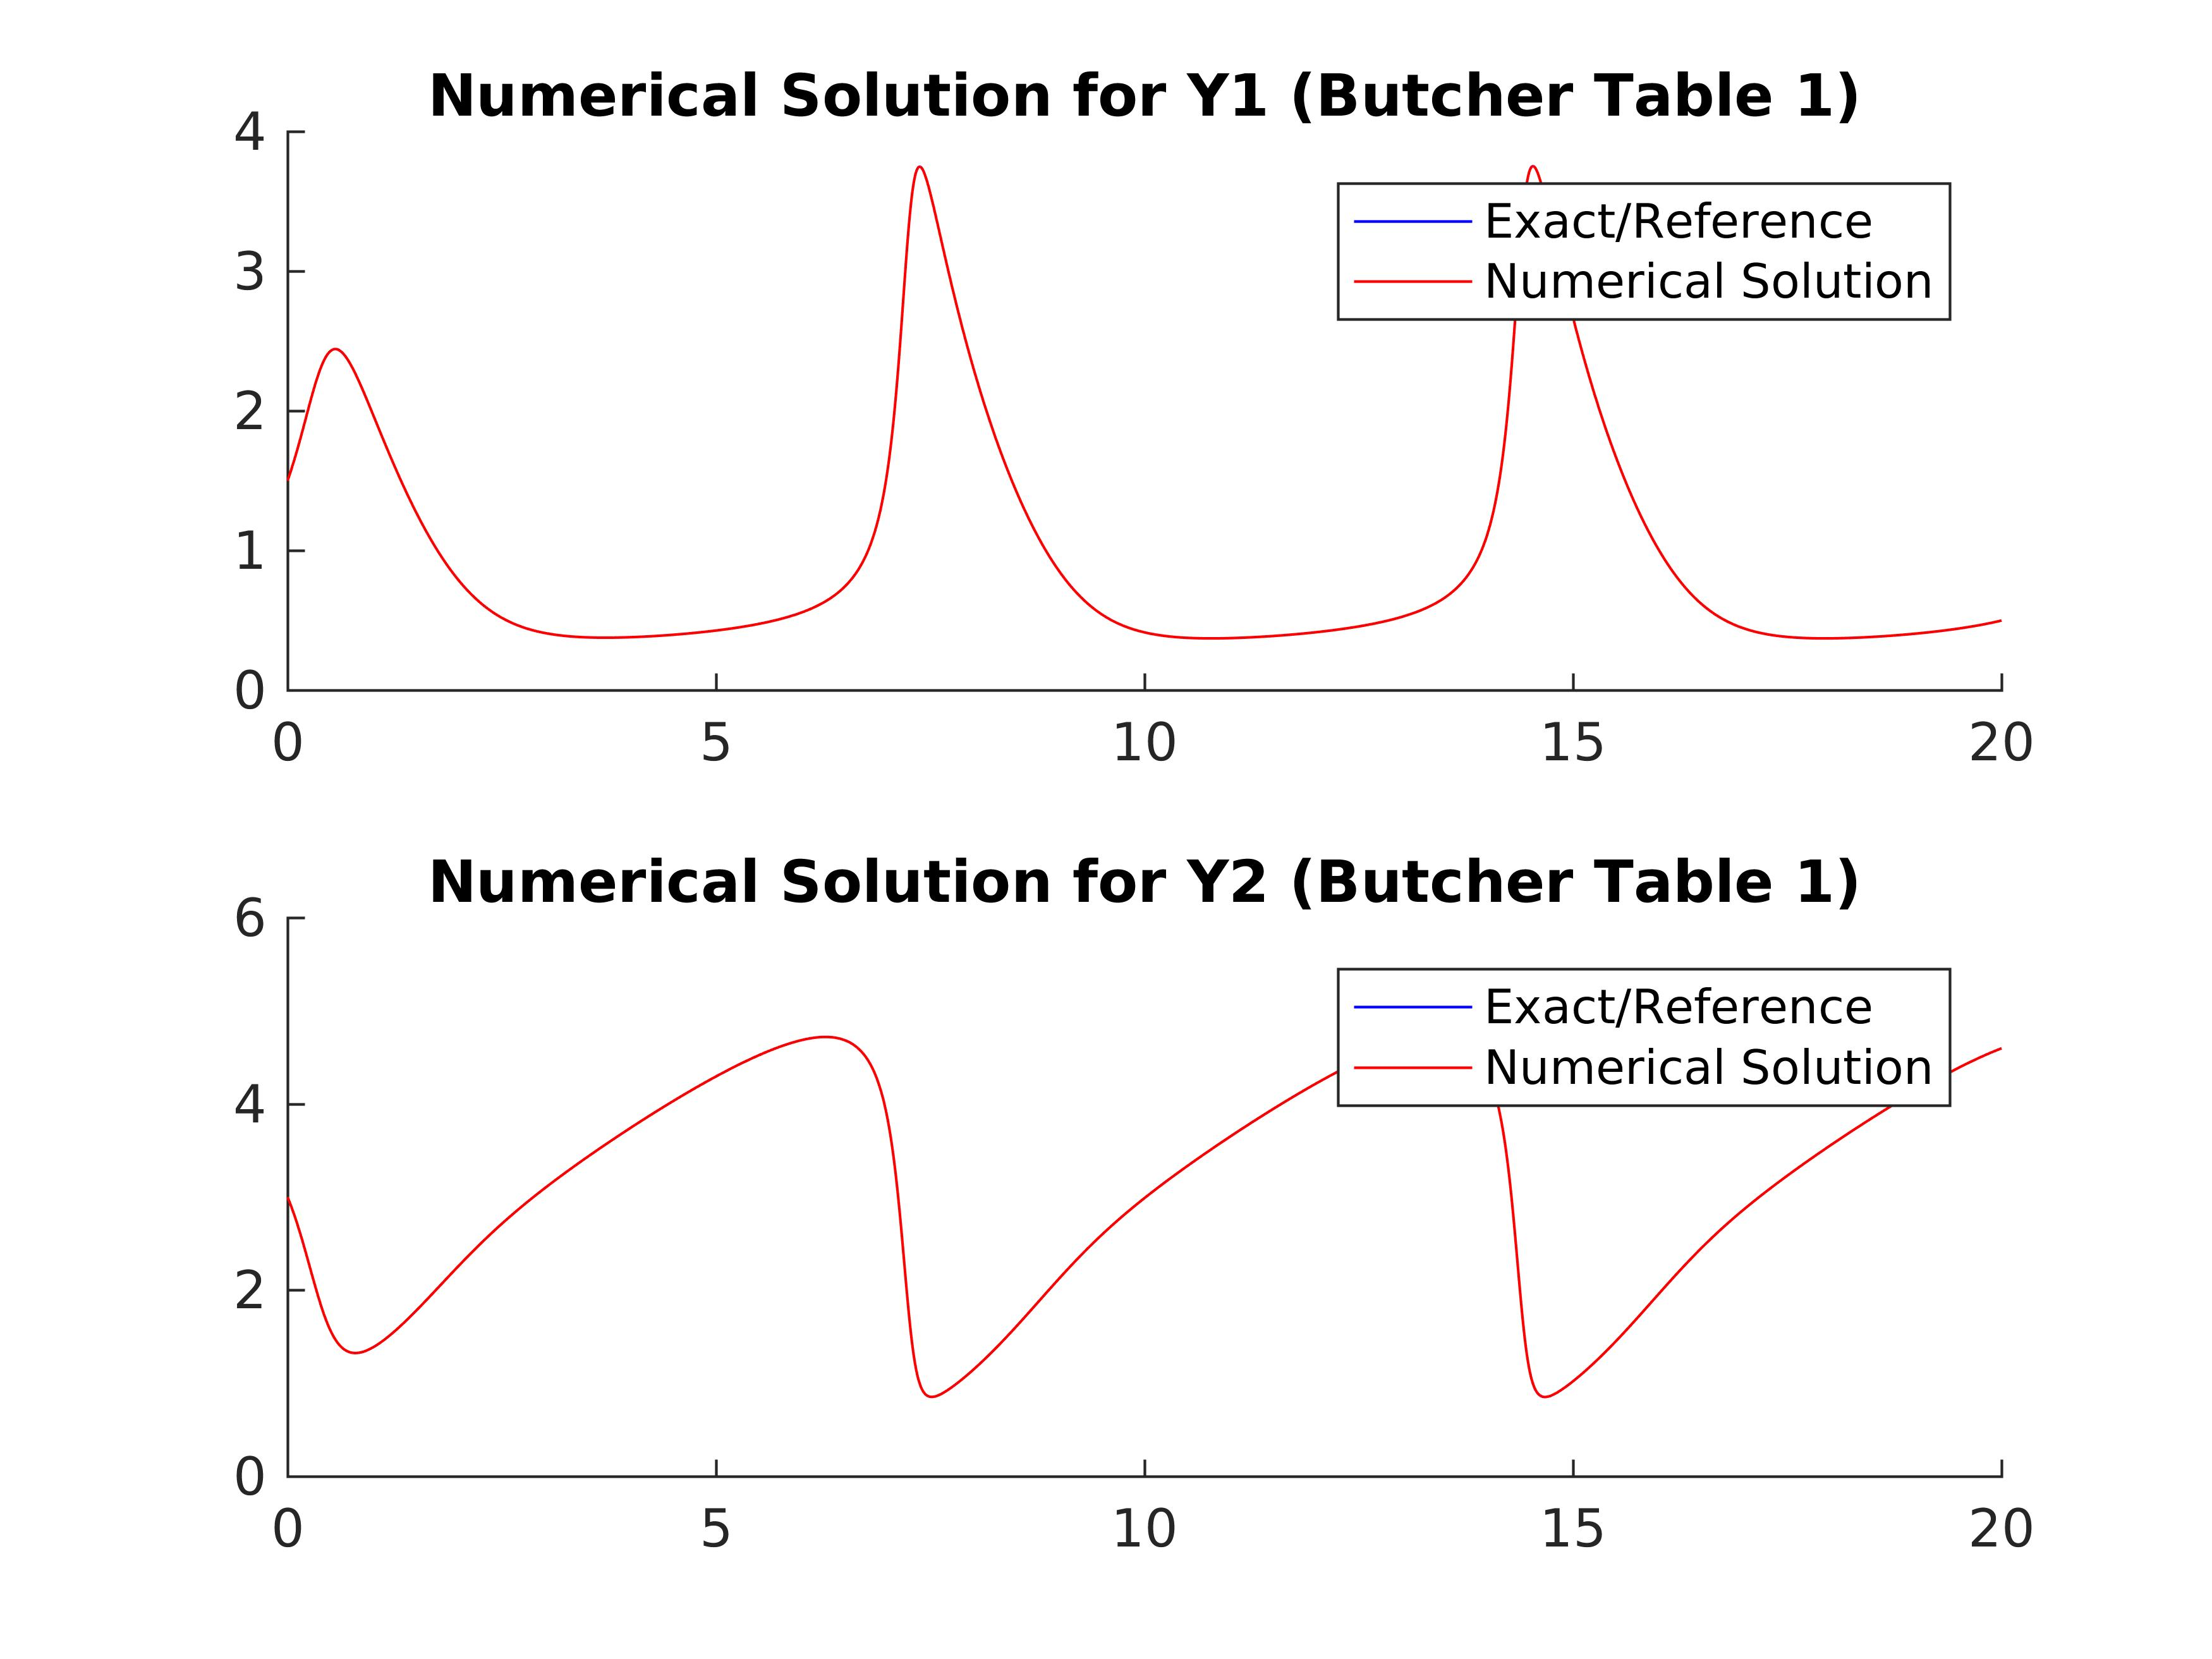
\includegraphics[scale=0.09]{1ns1}
\caption{\textsc{Numerical Solutions of Brusselator equation by Matlab.}}
\end{figure}
\begin{figure}[H]
\centering
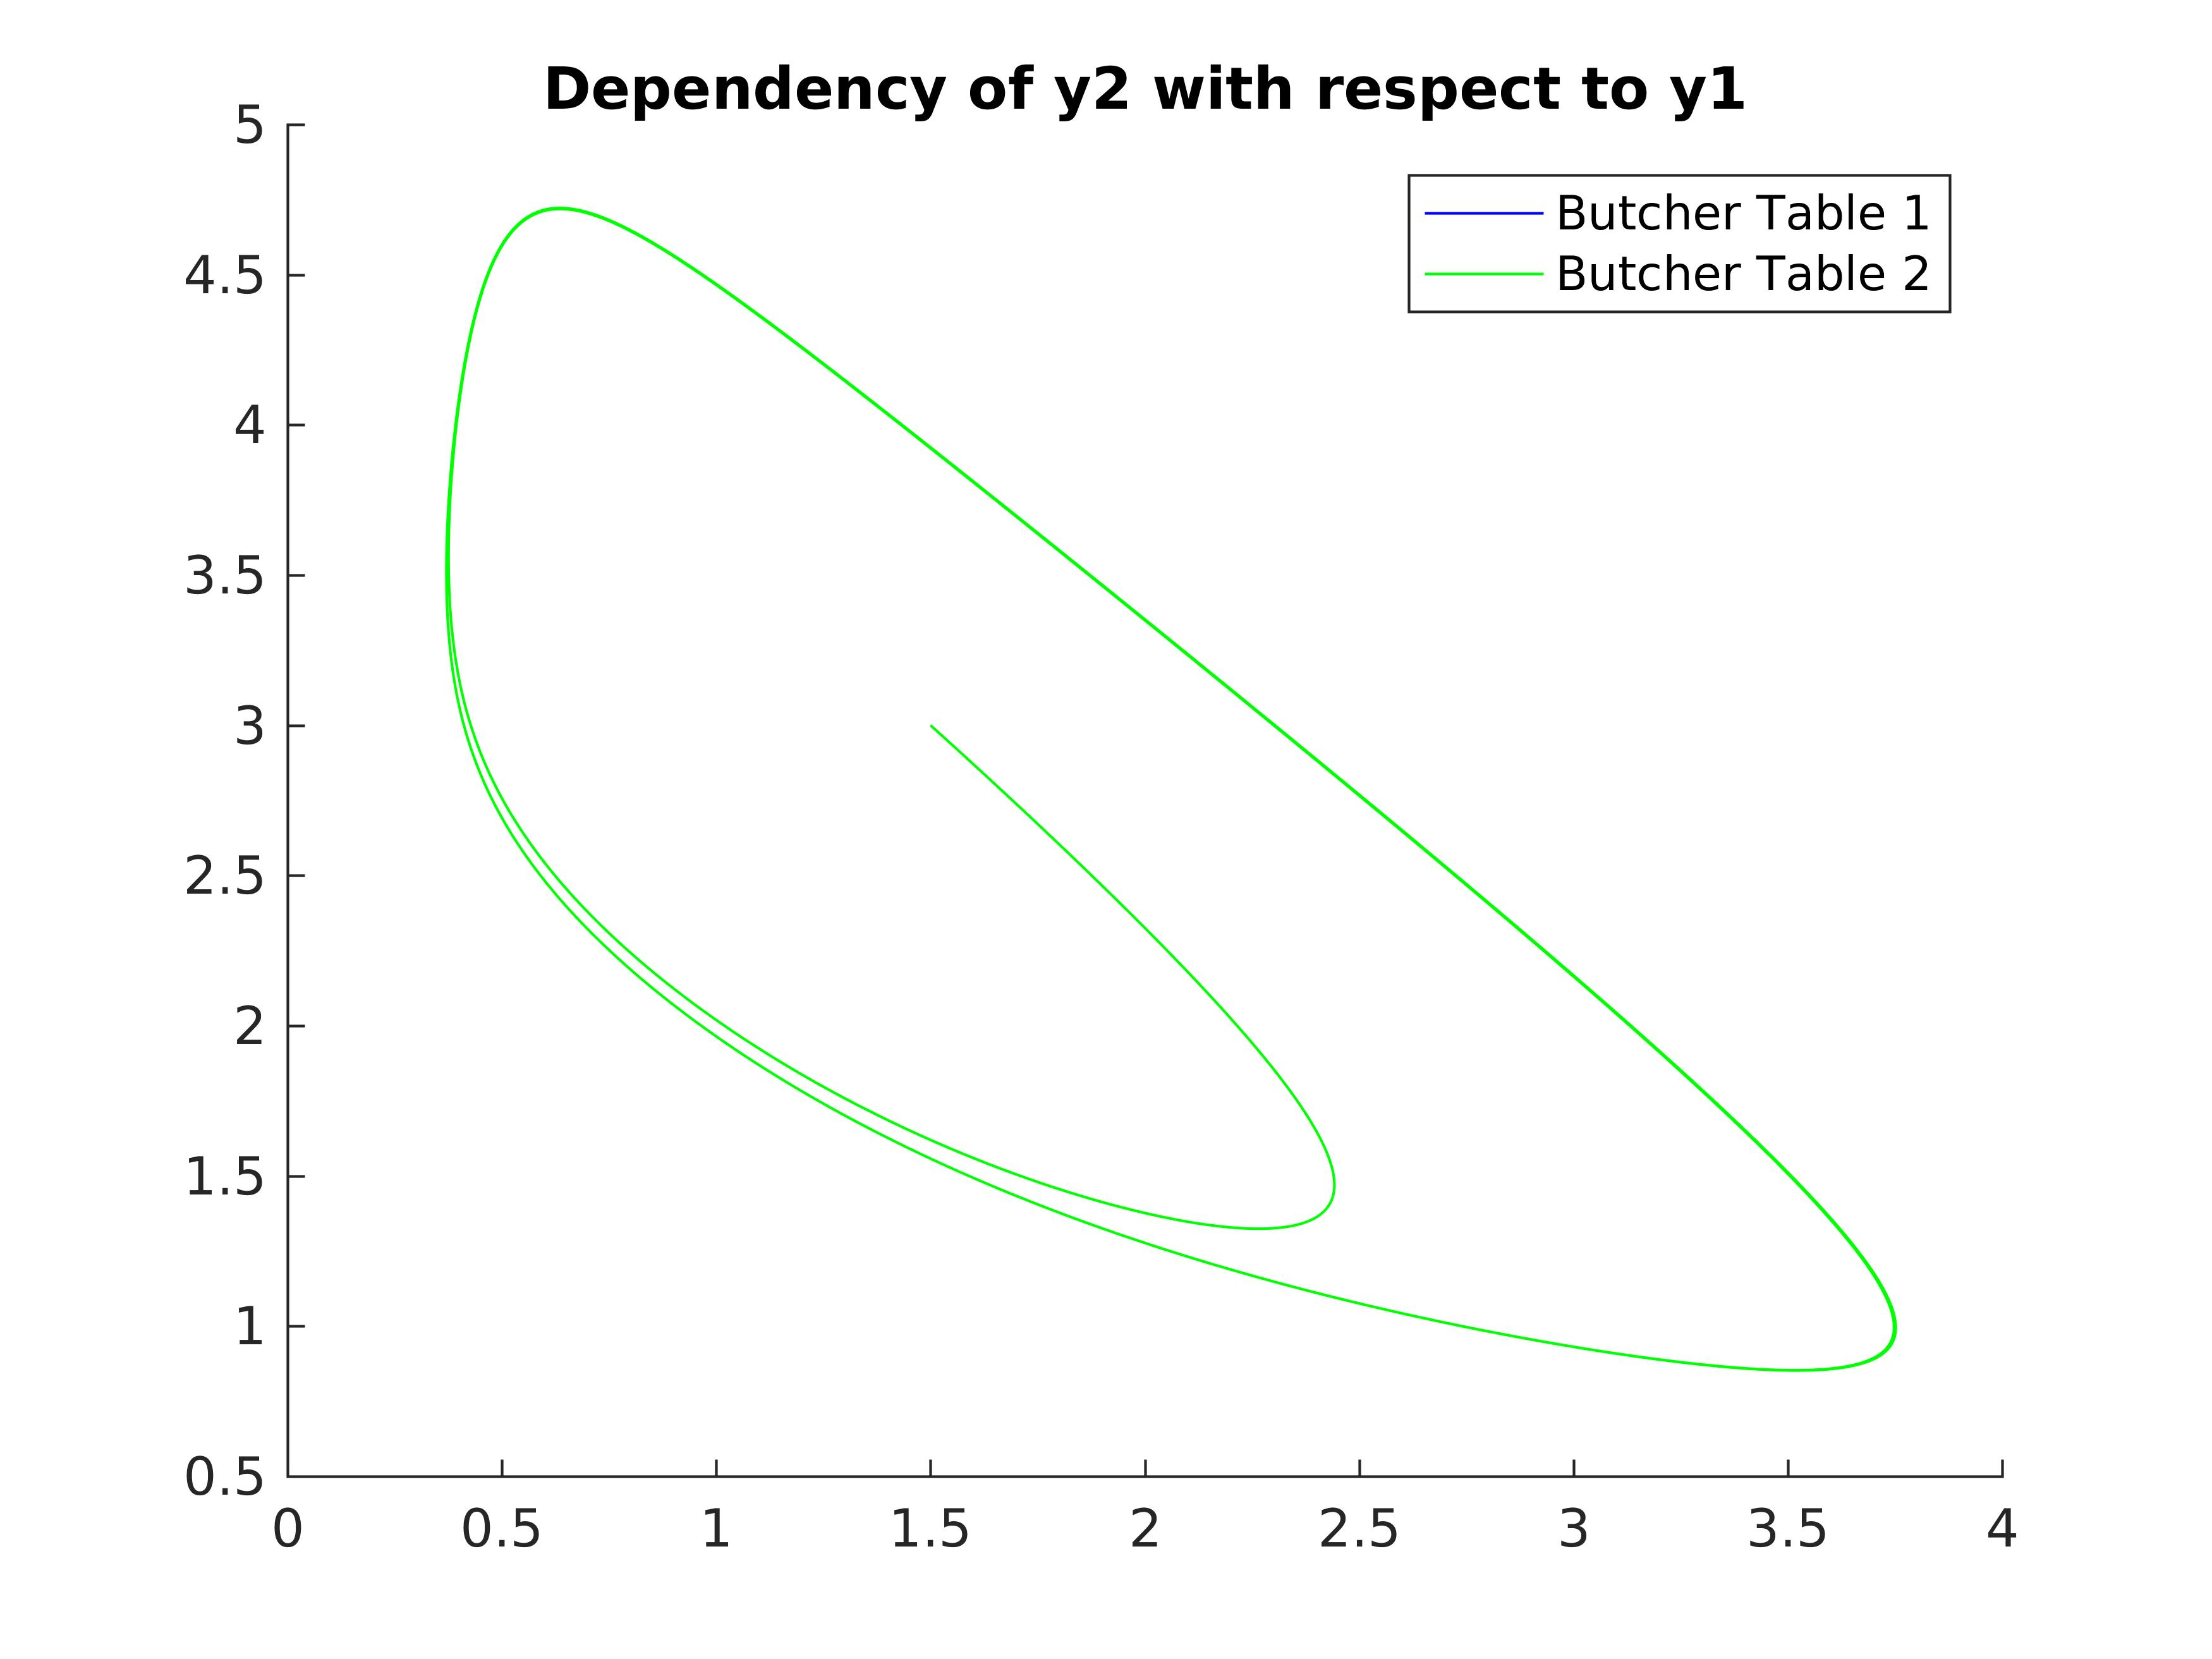
\includegraphics[scale=0.09]{1d}
\caption{\textsc{Dependency of $y_2$ with respect to $y_1$ of Brusselator equation by Matlab.}}
\end{figure}
\begin{figure}[H]
\centering
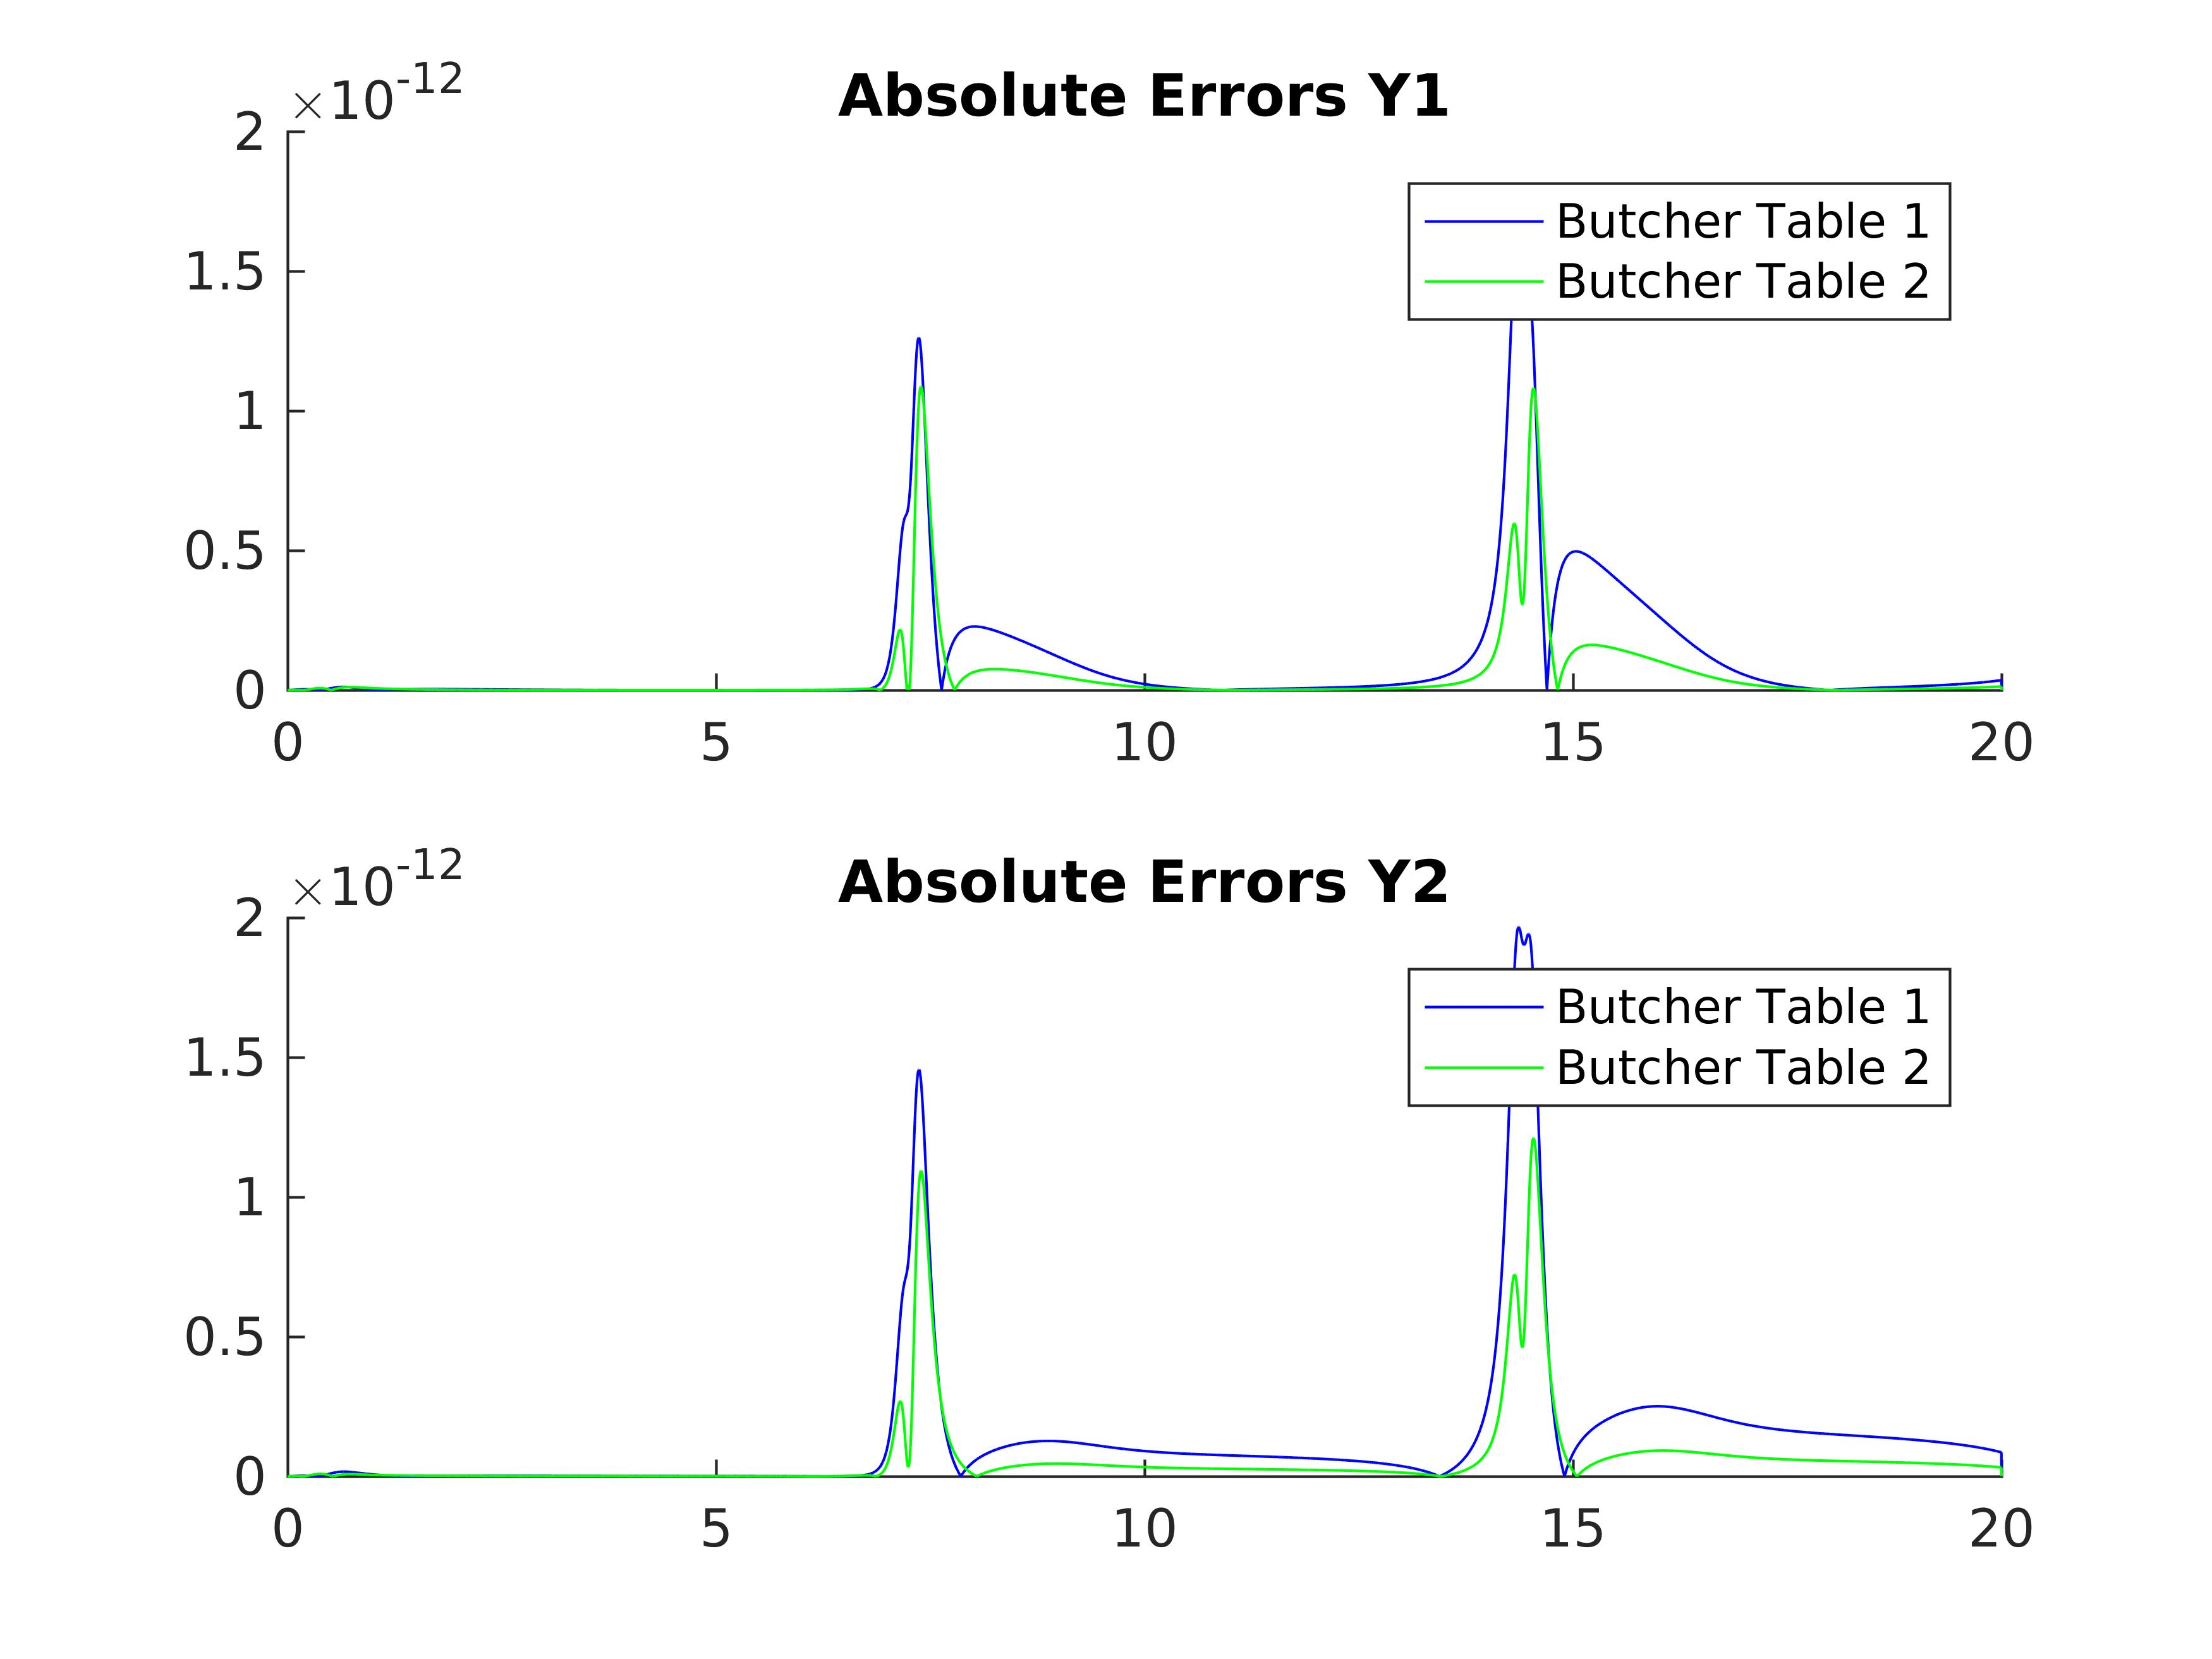
\includegraphics[scale=0.09]{1ae}
\caption{\textsc{Absolute Errors of Brusselator equation by Matlab.}}
\end{figure}
\begin{figure}[H]
\centering
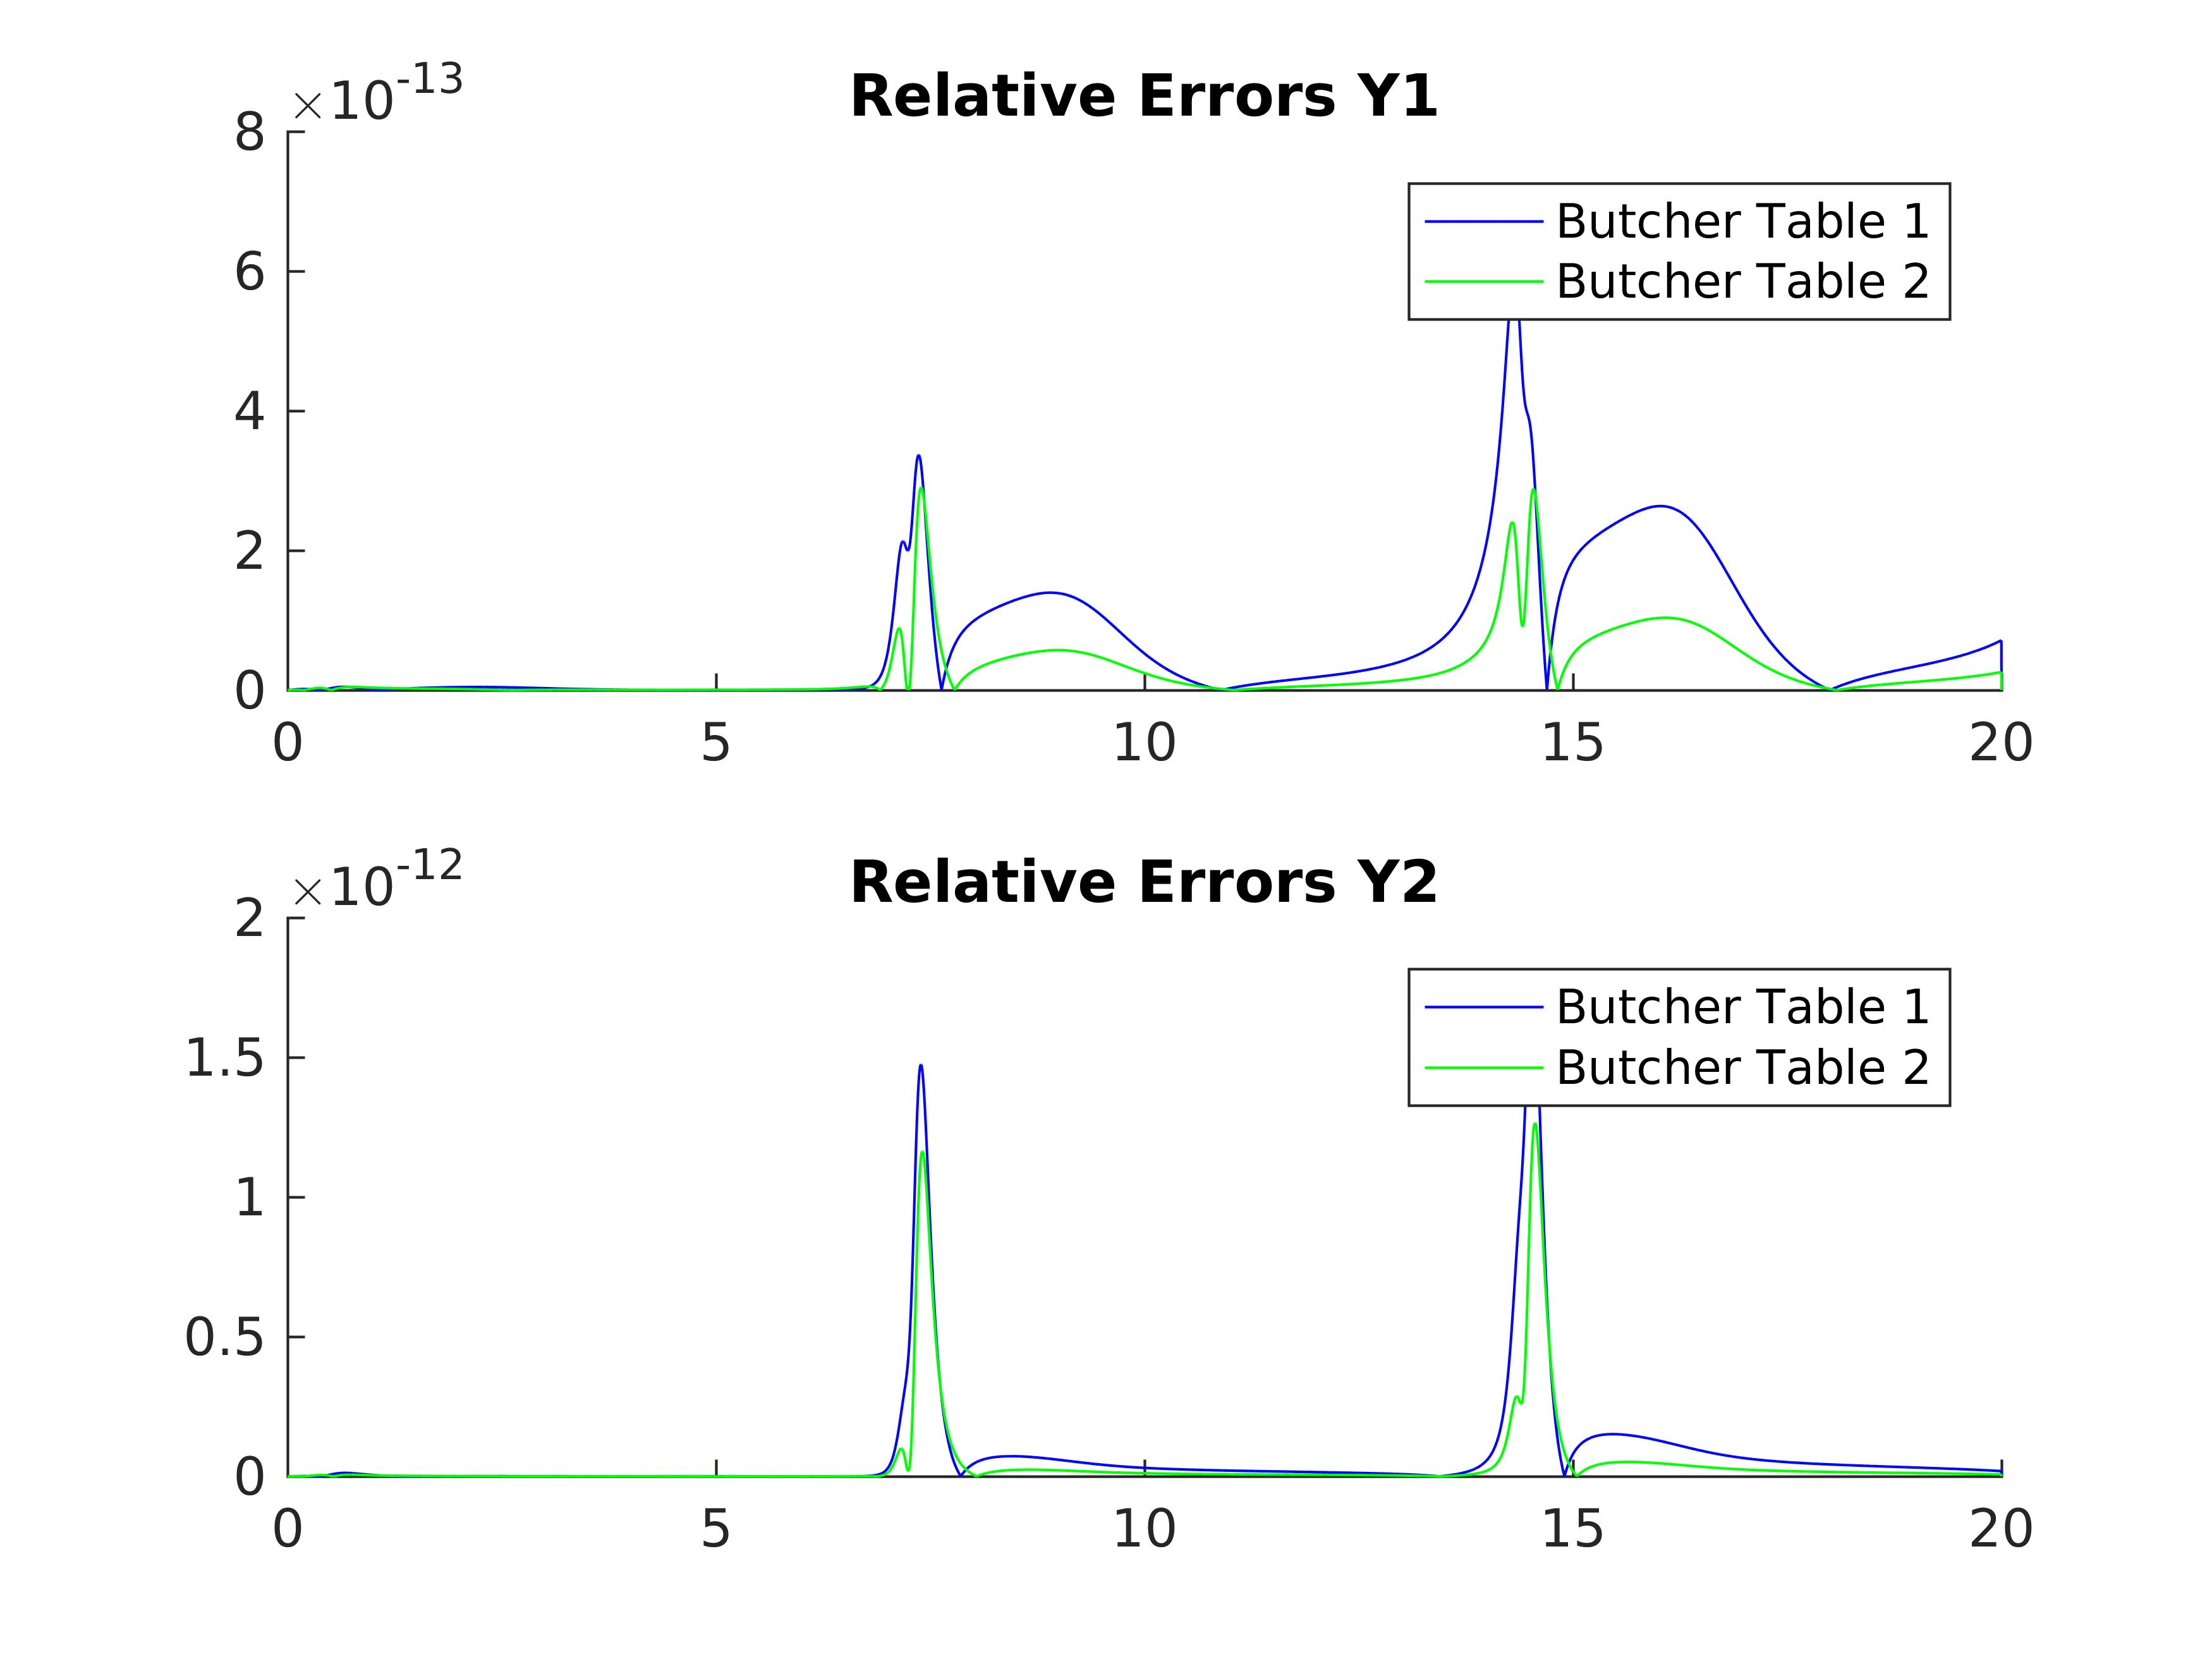
\includegraphics[scale=0.09]{1re}
\caption{\textsc{Relative Errors of Brusselator equation by Matlab.}}
\end{figure}
\subsection{\textsc{Fortran} Codes}
\subsubsection{b.f90}
\begin{lstlisting}
module b  
implicit none 
	integer, parameter :: dms=2 ! number of unknowns
    ! initial condition
	real (kind = 8), dimension(dms) :: x=(/1d0, 1d0/) 
    ! beginning and ending time points
	real (kind = 8) :: t=0d0,te=40d0 
	real (kind = 8) :: d=real(dms)
contains      
	subroutine f(t,y,f0)
		implicit none
		real (kind = 8), intent(in) :: t
		real (kind = 8), dimension(dms), intent(in) :: y
		real (kind = 8), dimension(dms), intent(out) :: f0
		
		f0(1)=1d0-4d0*y(1)+y(2)*(y(1)**2)
		f0(2)=3d0*y(1)-y(2)*(y(1)**2)
	end subroutine f
end module b 
\end{lstlisting}
\subsubsection{GNU Plot Results}
\begin{figure}[H]
\centering
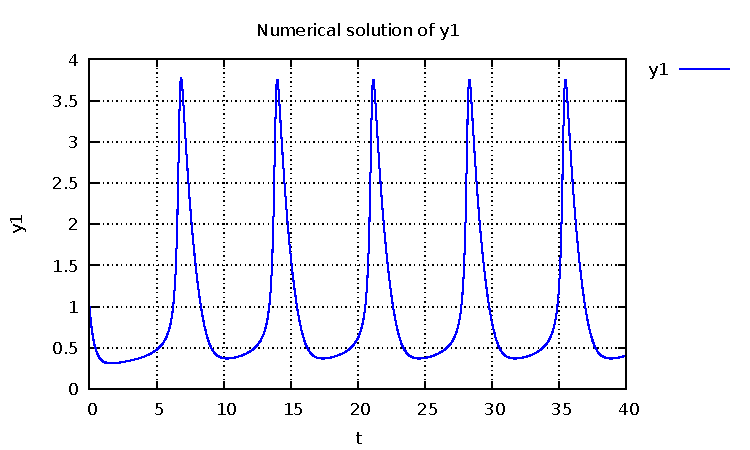
\includegraphics[scale=1.15]{b_1}
\caption{\textsc{Numerical Solution of $y_1$ of Brusselator equation by GNU Plot.}}
\end{figure}
\begin{figure}[H]
\centering
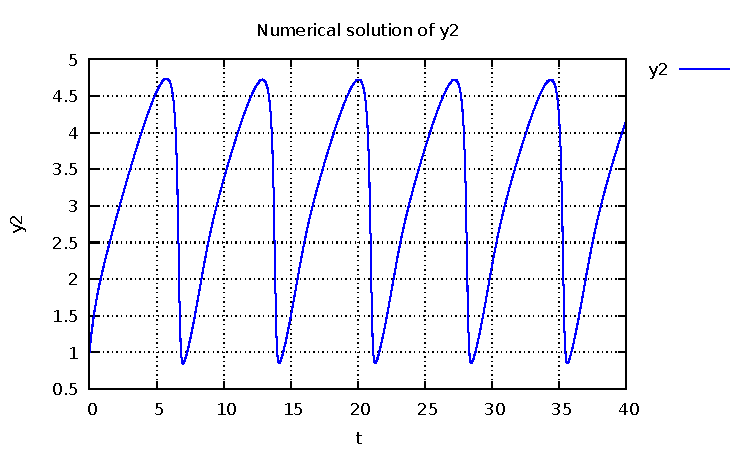
\includegraphics[scale=1.15]{b_2}
\caption{\textsc{Numerical Solution of $y_2$ of Brusselator equation by GNU Plot.}}
\end{figure}
\begin{figure}[H]
\centering
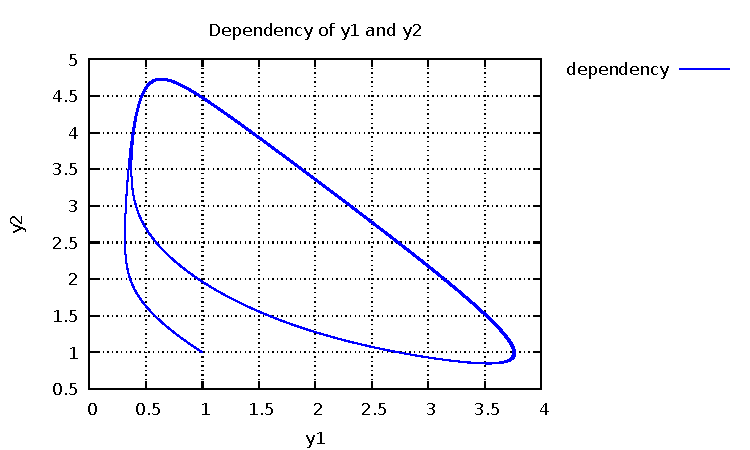
\includegraphics[scale=1.15]{b_d_1_2}
\caption{\textsc{Dependency of $y_1$ and $y_2$ of Brusselator equation by GNU Plot.}}
\end{figure}
\begin{figure}[H]
\centering
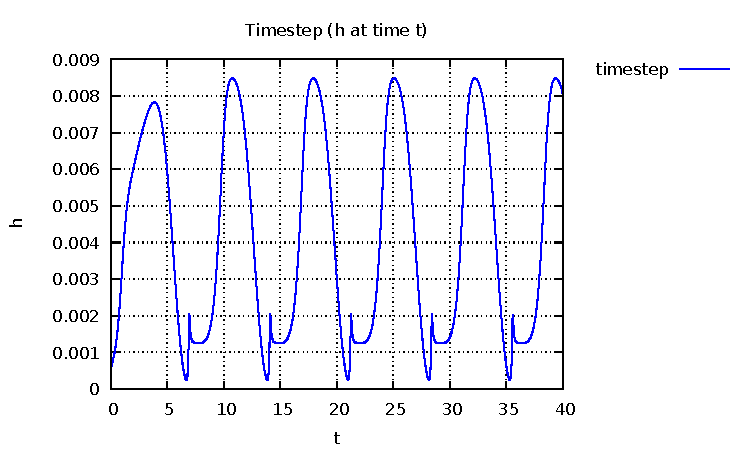
\includegraphics[scale=1.15]{b_ts}
\caption{\textsc{Timestep of Brusselator equation by GNU Plot.}}
\end{figure}
\section{Belousov-Zhabotinsky Reaction (BZ 2 ODEs)}
\textsc{BZ 2 ODEs (Belousov-Zhabotinsky reaction).} \index{Belousov–Zhabotinsky reaction}
\begin{align}
    \dfrac{db}{dt}  &=  \dfrac{1}{\epsilon} \left( b\left(1-b\right) + fc\dfrac{q-b}{q+b} \right)
    \\
    \dfrac{dc}{dt}  &=  b-c
\end{align}
where $y_1\left(0\right) = 0.04$, $y_2\left(0\right) = 0.1$, where the coefficients are given by $f = \dfrac{2}{3}$, $q = 8\cdot 10^{-4}$ and $\epsilon = 4\cdot 10^{-2}$.\\
\\
\textsc{Applications.}
\begin{itemize}
\item A classical example of non-equilibrium thermodynamics, resulting in the establishment of a nonlinear chemical oscillator.
\item An interesting chemical model of nonequilibrium biological phenomena.
\item Mathematical models of the Belousov-Zhabotinsky reactions are of theoretical interest and simulations.
\end{itemize}

\subsection{\textsc{Fortran} Codes}
\begin{lstlisting}
module bz2  
implicit none 
	integer, parameter :: dms=2 ! number of unknowns
	! initial condition
	real (kind = 8), dimension(dms) :: x=(/1d-5, 1d-5/)
	! beginning and ending time points 
	real (kind = 8) :: t=0d0,te=40d0 
	real (kind = 8) :: d=real(dms)
contains      
	subroutine f(t,y,f0)
		implicit none
		real (kind = 8), intent(in) :: t
		real (kind = 8), dimension(dms), intent(in) :: y
		real (kind = 8), dimension(dms), intent(out) :: f0
		
		f0(1)=(y(1)*(1-y(1))+2/3d0*y(2)*(8d-4-y(1))/(8d-4+y(1)))*0.25d+2
		f0(2)=y(1)-y(2)
	end subroutine f
end module bz2
\end{lstlisting}
\subsubsection{GNU Plot Results}
\begin{figure}[H]
\centering
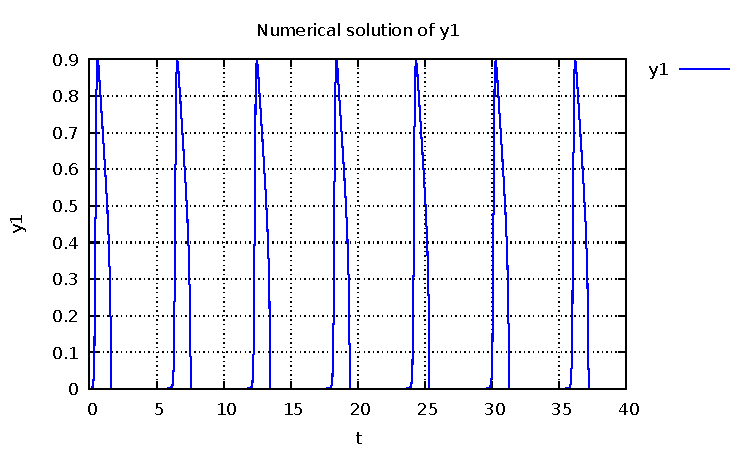
\includegraphics[scale=1.1]{bz2_1}
\caption{\textsc{Numerical Solution of $y_1$ of BZ 2 ODEs by GNU Plot.}}
\end{figure}
\begin{figure}[H]
\centering
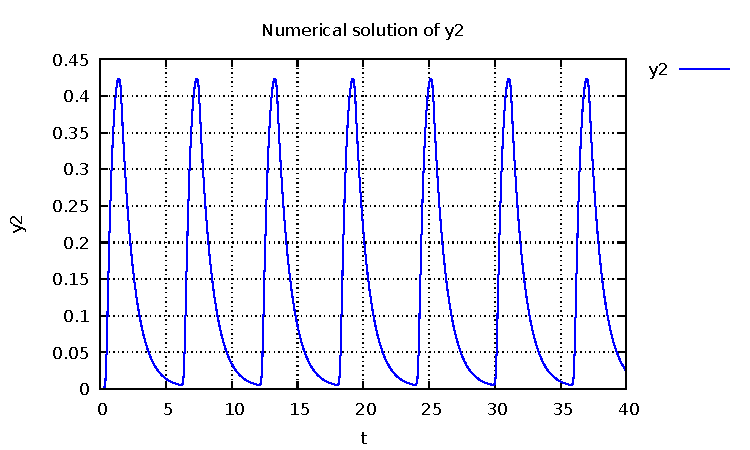
\includegraphics[scale=1.1]{bz2_2}
\caption{\textsc{Numerical Solution of $y_2$ of BZ 2 ODEs by GNU Plot.}}
\end{figure}
\begin{figure}[H]
\centering
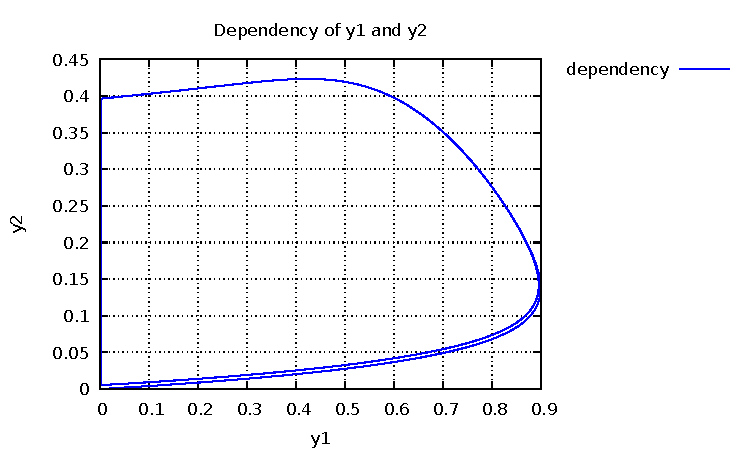
\includegraphics[scale=1.1]{bz2_d_1_2}
\caption{\textsc{Dependency of $y_1$ and $y_2$ of BZ 2 ODEs by GNU Plot.}}
\end{figure}
\begin{figure}[H]
\centering
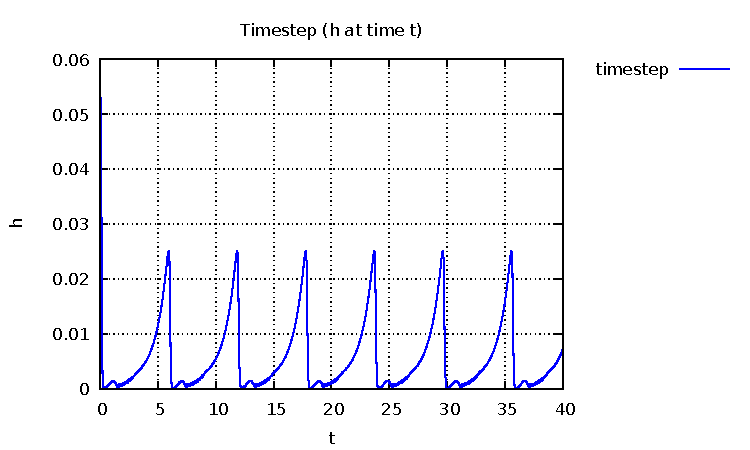
\includegraphics[scale=1.1]{bz2_ts}
\caption{\textsc{Timestep of BZ 2 ODEs by GNU Plot.}}
\end{figure}

\section{Oregonator}
\textsc{Oregonator.} \index{Oregonator}
\begin{align}
    \dfrac{dy_1}{dt}  &=  77.27 \left(y_2  +  y_1 \left(1 - 8.375*10^{-6} y_1 - y_2\right) \right)
    \\
    \dfrac{dy_2}{dt}  &=  \dfrac{y_3 - \left(1+y_1\right)y_2}{77.27}
    \\
    \dfrac{dy_3}{dt}  &=  0.161\left(y_1-y_3\right)
\end{align}
where $y_1\left(0\right) = 1$, $y_2\left(0\right) = 2$ and $y_3\left(0\right) = 3$.\\
\\
\textsc{Applications.}
\begin{itemize}
\item A theoretical model for a type of autocatalytic reaction.
\item The simplest realistic model of the chemical dynamics of the oscillatory Belousov-Zhabotinsky reaction.
\item A reduced model of the FKN mechanism (developed by Richard Field, Endre K\"{o}r\"{o}s, and Richard M. Noyes).
\end{itemize}
\subsection{\textsc{Fortran} Codes}
\begin{lstlisting}
module o  
implicit none 
	integer, parameter :: dms=3 ! number of unknowns
	! initial condition
	real (kind = 8), dimension(dms) :: x=(/1d0, 2d0, 3d0/) 
    ! beginning and ending time points
	real (kind = 8) :: t=0d0,te=1200d0 
	real (kind = 8) :: d=real(dms)
contains      
	subroutine f(t,y,f0)
		implicit none
		real (kind = 8), intent(in) :: t
		real (kind = 8), dimension(dms), intent(in) :: y
		real (kind = 8), dimension(dms), intent(out) :: f0
		
		f0(1)=77.27d0*(y(2)+y(1)*(1-8.375d-6*y(1)-y(2)))
		f0(2)=(y(3)-(1+y(1))*y(2))/77.27d0
		f0(3)=0.161d0*(y(1)-y(3))
	end subroutine f
end module o 
\end{lstlisting}
\subsubsection{GNU Plot Results}
\begin{figure}[H]
\centering
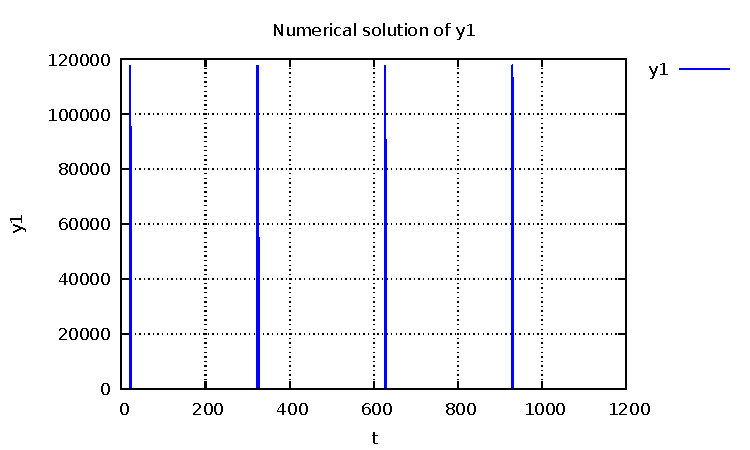
\includegraphics[scale=1.1]{o_1}
\caption{\textsc{Numerical Solution of $y_1$ of  Oregonator equation by GNU Plot.}}
\end{figure}
\begin{figure}[H]
\centering
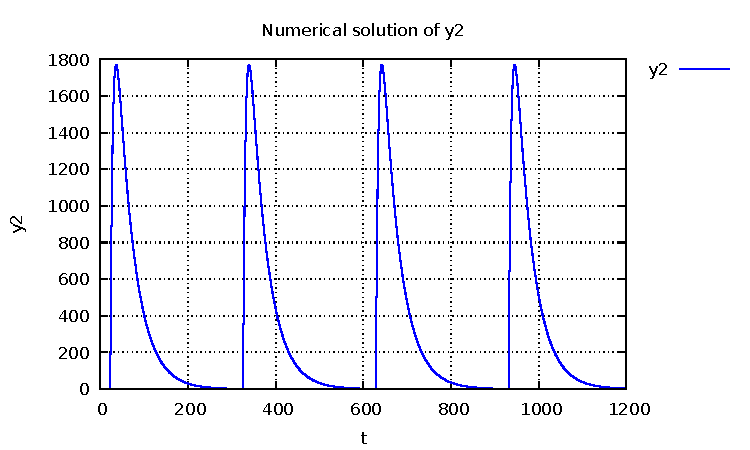
\includegraphics[scale=1.1]{o_2}
\caption{\textsc{Numerical Solution of $y_2$ of  Oregonator equation by GNU Plot.}}
\end{figure}
\begin{figure}[H]
\centering
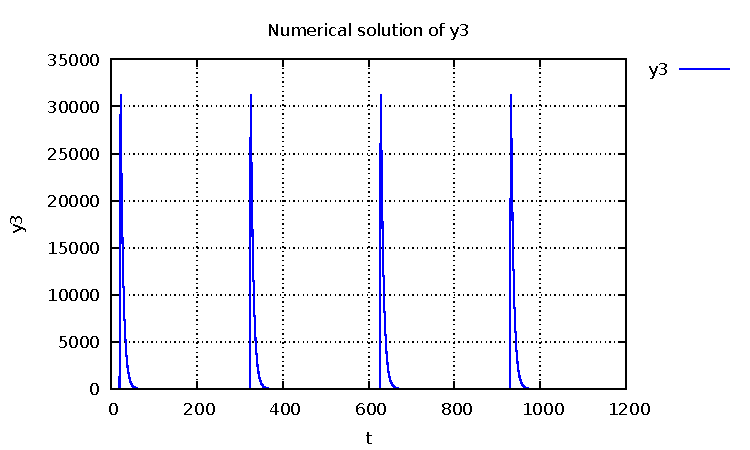
\includegraphics[scale=1.1]{o_3}
\caption{\textsc{Numerical Solution of $y_3$ of  Oregonator equation by GNU Plot.}}
\end{figure}
\begin{figure}[H]
\centering
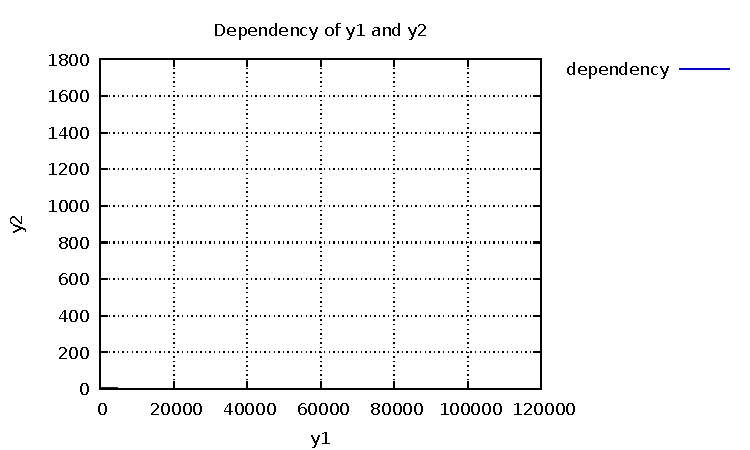
\includegraphics[scale=1.1]{o_d_1_2}
\caption{\textsc{Dependency of $y_1$ and $y_2$ of Oregonator equation by GNU Plot.}}
\end{figure}
\begin{figure}[H]
\centering
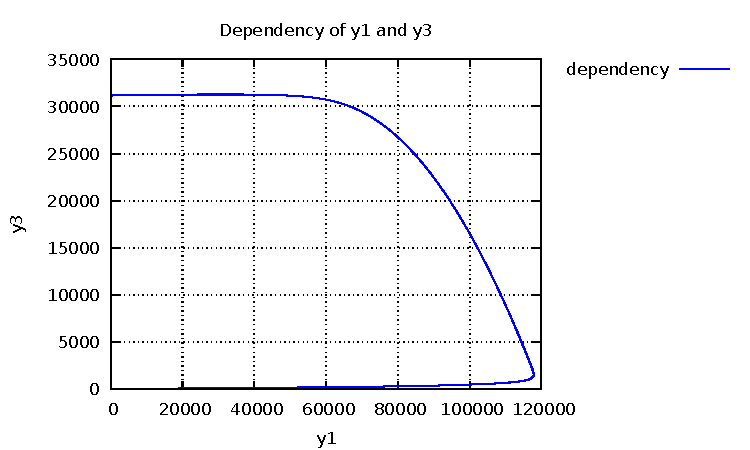
\includegraphics[scale=1.1]{o_d_1_3}
\caption{\textsc{Dependency of $y_1$ and $y_3$ of Oregonator equation by GNU Plot.}}
\end{figure}
\begin{figure}[H]
\centering
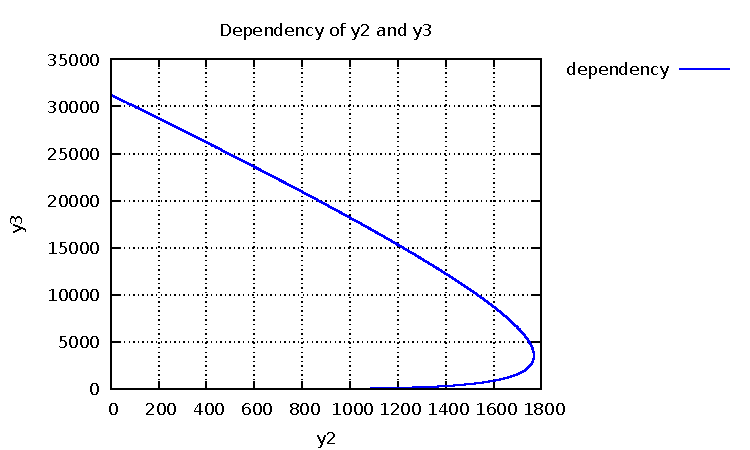
\includegraphics[scale=1.1]{o_d_2_3}
\caption{\textsc{Dependency of $y_2$ and $y_3$ of Oregonator equation by GNU Plot.}}
\end{figure}
\begin{figure}[H]
\centering
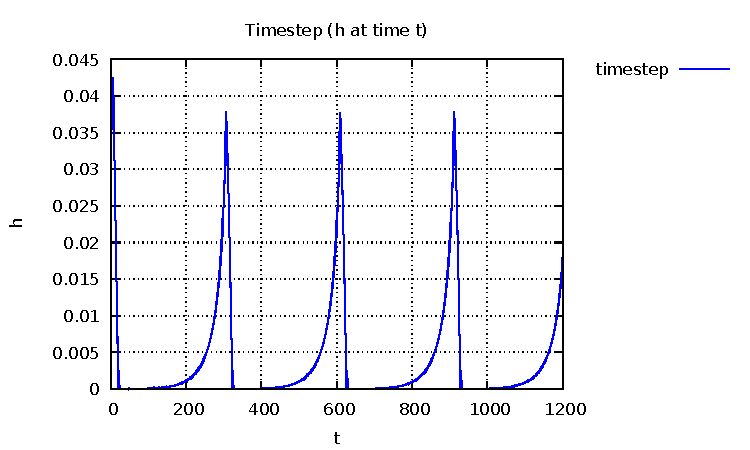
\includegraphics[scale=1.1]{o_ts}
\caption{\textsc{Timestep of Oregonator equation by GNU Plot.}}
\end{figure}
\section{Belousov-Zhabotinsky Reaction (BZ 3 ODEs)}
\textsc{BZ 3 ODEs (Belousov-Zhabotinsky reaction).}
\begin{align}
    \dfrac{da}{dt}  &=  \dfrac{1}{\mu} \left(-qa -ab + fc\right)
    \\
    \dfrac{db}{dt}  &=  \dfrac{1}{\epsilon} \left(qa -ab + b - b^2\right)
    \\
    \dfrac{dc}{dt}  &=  b-c
\end{align}
where $y_1\left(0\right) = 10$, $y_2\left(0\right) = 0.04$, $y_3\left(0\right) = 0.1$, where the coefficients are given by $f = \dfrac{2}{3}$, $q = 8\cdot 10^{-4}$, $\mu=10^{-6}$ and $\epsilon = 4\cdot 10^{-2}$.
\subsection{\textsc{Fortran} Codes}
\begin{lstlisting}
module bz3
implicit none 
	integer, parameter :: dms=3 ! number of unknowns
	! initial condition
	real (kind = 8), dimension(dms) :: x=(/1d-5, 1d-5, 1d-5/) 
	! beginning and ending time points
	real (kind = 8) :: t=0d0,te=40d0 
	real (kind = 8) :: d=real(dms)
contains      
	subroutine f(t,y,f0)
		implicit none
		real (kind = 8), intent(in) :: t
		real (kind = 8), dimension(dms), intent(in) :: y
		real (kind = 8), dimension(dms), intent(out) :: f0
		
		f0(1)=(4d-4*y(2)-y(1)*y(2)+y(1)*(1-y(1)))*0.25d+2
		f0(2)=(-4d-4*y(2)-y(1)*y(2)+(2/3d0)*y(3))*0.25d+4
		f0(3)=y(1)-y(3)
	end subroutine f
end module bz3
\end{lstlisting}
\subsubsection{GNU Plot Results}
\begin{figure}[H]
\centering
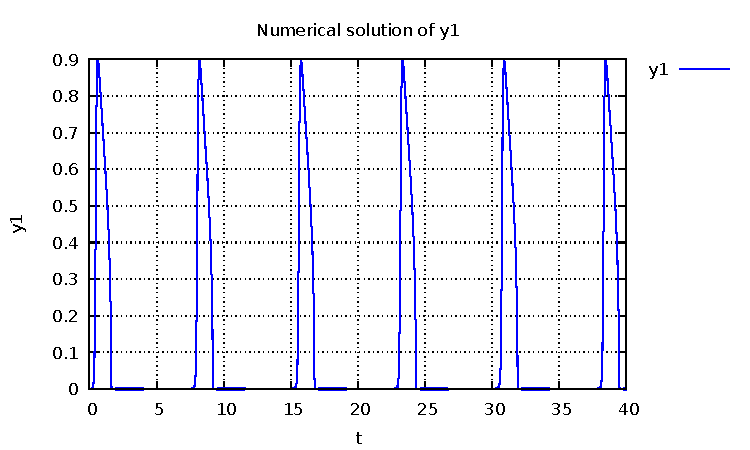
\includegraphics[scale=1.1]{bz3_1}
\caption{\textsc{Numerical Solution of $y_1$ of BZ 3 ODEs by GNU Plot.}}
\end{figure}
\begin{figure}[H]
\centering
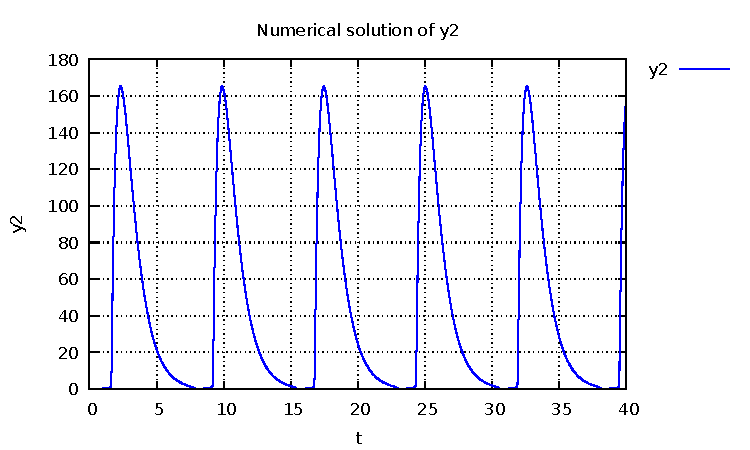
\includegraphics[scale=1.1]{bz3_2}
\caption{\textsc{Numerical Solution of $y_2$ of BZ 3 ODEs by GNU Plot.}}
\end{figure}
\begin{figure}[H]
\centering
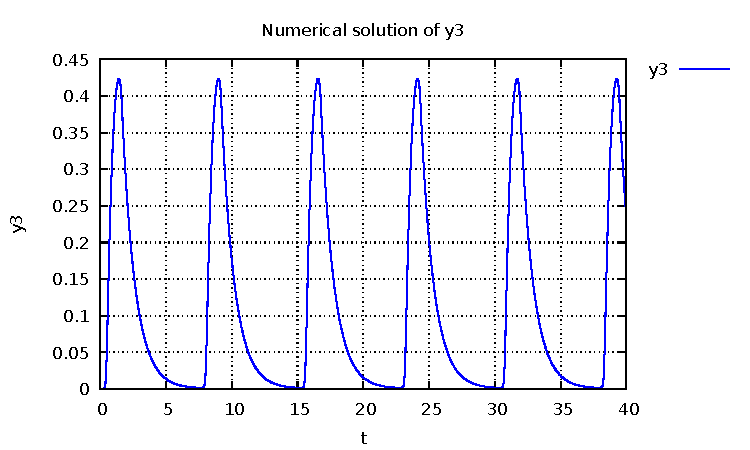
\includegraphics[scale=1.1]{bz3_3}
\caption{\textsc{Numerical Solution of $y_3$ of BZ 3 ODEs by GNU Plot.}}
\end{figure}
\begin{figure}[H]
\centering
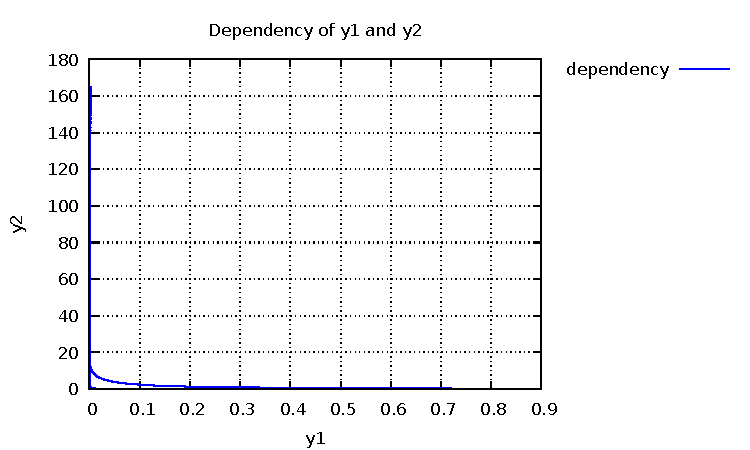
\includegraphics[scale=1.1]{bz3_d_1_2}
\caption{\textsc{Dependency of $y_1$ and $y_2$ of BZ 3 ODEs by GNU Plot.}}
\end{figure}
\begin{figure}[H]
\centering
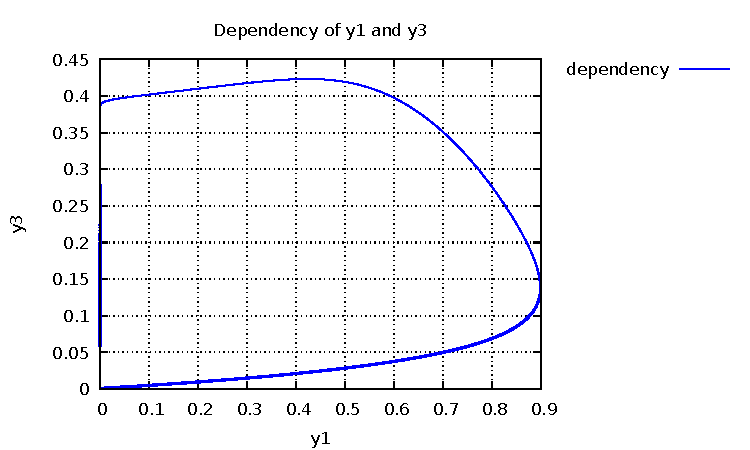
\includegraphics[scale=1.1]{bz3_d_1_3}
\caption{\textsc{Dependency of $y_1$ and $y_3$ of BZ 3 ODEs by GNU Plot.}}
\end{figure}
\begin{figure}[H]
\centering
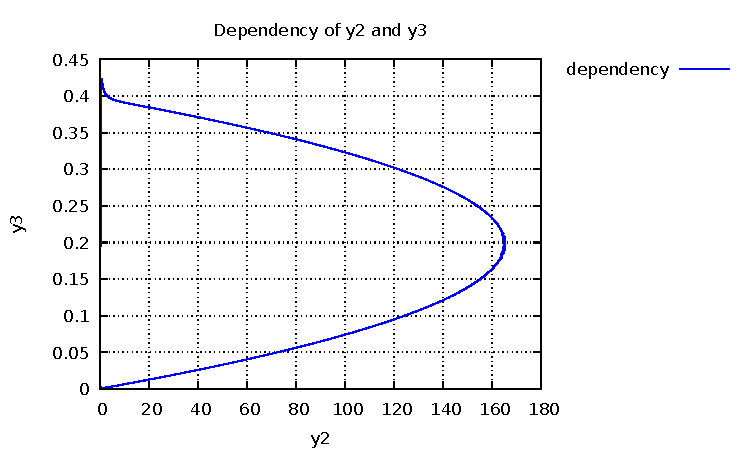
\includegraphics[scale=1.1]{bz3_d_2_3}
\caption{\textsc{Dependency of $y_2$ and $y_3$ of BZ 3 ODEs by GNU Plot.}}
\end{figure}
\begin{figure}[H]
\centering
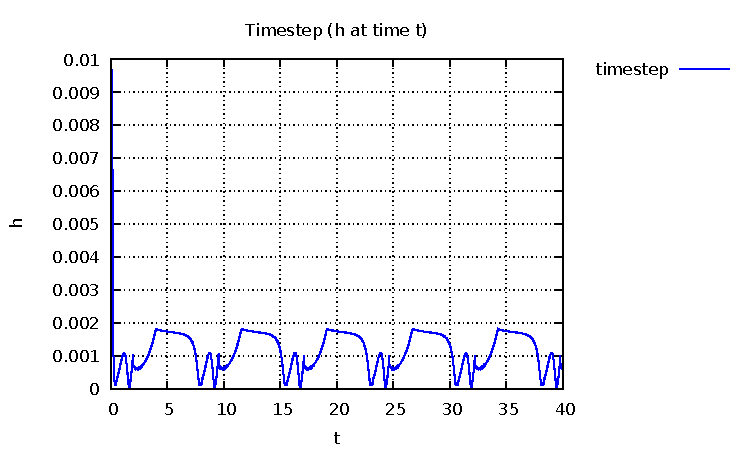
\includegraphics[scale=1.1]{bz3_ts}
\caption{\textsc{Timestep of BZ 3 ODEs by GNU Plot.}}
\end{figure}



\section{van der Pol Equation}
\textsc{van der Pol equations.} \index{van der Pol equation}
\begin{align}
    \dfrac{dy_1}{dt}  &=  y_2
    \\
    \dfrac{dy_2}{dt}  &=  [ (1-y_1^2)y_2 - y_1 ] / \epsilon
\end{align}
where $\epsilon = 10^{-6}$.\\
\\
\textsc{Applications.} A basic model for oscillatory processes in physics, electronics, biology, neurology, sociology and economics
\begin{itemize}
\item \textbf{Physics.} Models \textbf{electrical circuits connected with triod oscillators}. A prototype for systems with self-excited limit cycle oscillations.
\item \textbf{Medicine.} Study the range of stability of heart dynamics. Situation in which a real heart is driven by a pacemaker. Stabilize a heart's irregular beating.
\item textbf{Biology.} The basis of a model of coupled neurons in the gastric mill circuit of the stomatogastric ganglion.
\item \textbf{Seismology.} Used in the development a model of the interaction of two plates in a geological fault.
\end{itemize}
\subsection{\textsc{Fortran} Codes}
\begin{lstlisting}
module vdp  
implicit none 
	integer, parameter :: dms=2 ! number of unknowns
    ! initial condition
	real (kind = 8), dimension(dms) :: x=(/2d0, -0.66d0/) 
    ! beginning and ending time points
	real (kind = 8) :: t=0d0,te=2d0 
	real (kind = 8) :: d=real(dms)
contains      
	subroutine f(t,y,f0)
		implicit none
		real (kind = 8), intent(in) :: t
		real (kind = 8), dimension(dms), intent(in) :: y
		real (kind = 8), dimension(dms), intent(out) :: f0
		
		f0(1)=y(2)
		f0(2)=(((1-(y(1)**2))*y(2))-y(1))*1d+6
	end subroutine f
end module vdp 
\end{lstlisting}

\subsubsection{GNU Plot Results}
\begin{figure}[H]
\centering
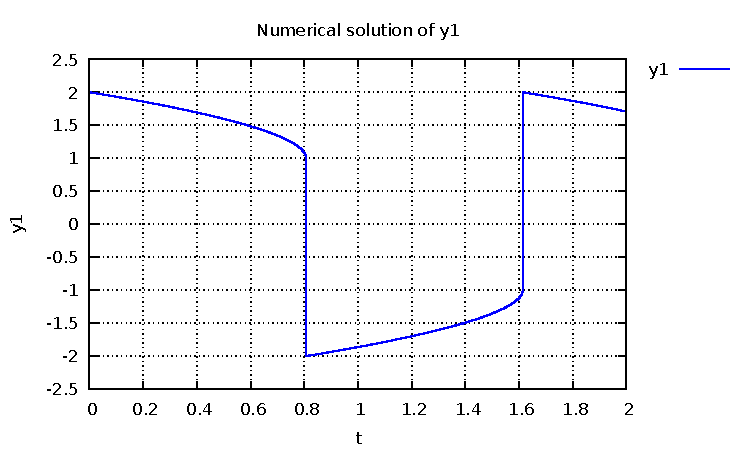
\includegraphics[scale=1.1]{vdp_1}
\caption{\textsc{Numerical Solution of $y_1$ of van der Pol equation by GNU Plot.}}
\end{figure}
\begin{figure}[H]
\centering
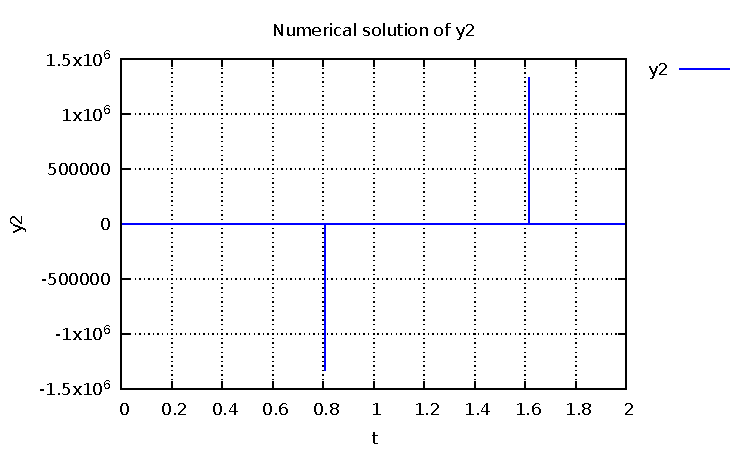
\includegraphics[scale=1.1]{vdp_2}
\caption{\textsc{Numerical Solution of $y_2$ of van der Pol equation by GNU Plot.}}
\end{figure}
\begin{figure}[H]
\centering
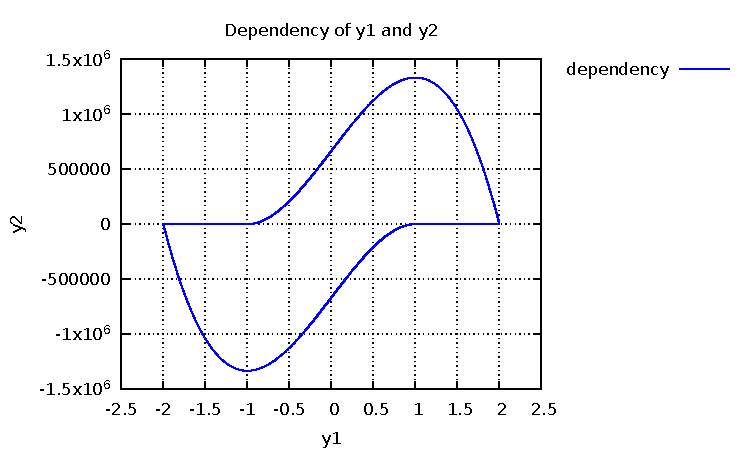
\includegraphics[scale=1.1]{vdp_d_1_2}
\caption{\textsc{Dependency of $y_1$ and $y_2$ of van der Pol equation by GNU Plot.}}
\end{figure}
\begin{figure}[H]
\centering
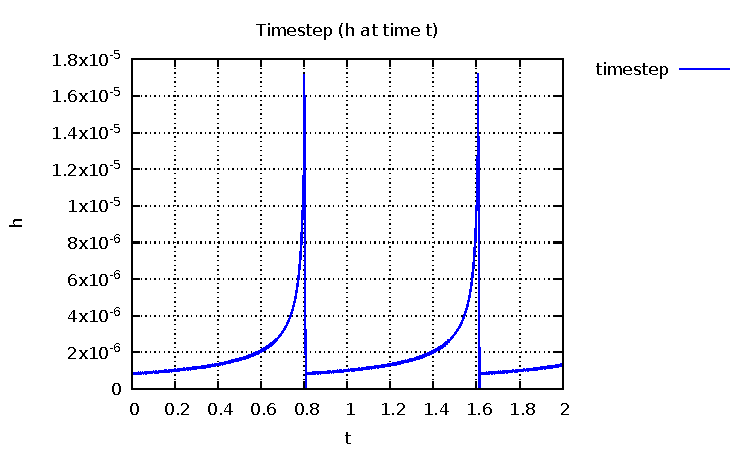
\includegraphics[scale=1.1]{vdp_ts}
\caption{\textsc{Timestep of van der Pol equation by GNU Plot.}}
\end{figure}

\section{Bonus Problems}
See \textsc{Fortran} routine \texttt{customf.f90}.
\begin{figure}[H]
\centering
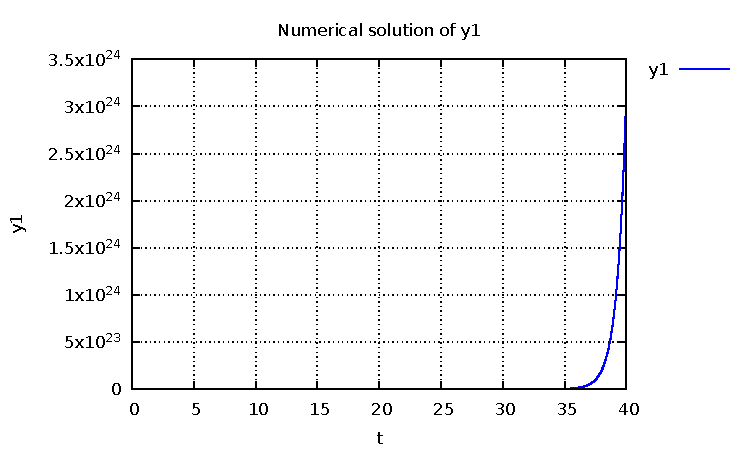
\includegraphics[scale=1.1]{f_1}
\caption{\textsc{Numerical Solution of $y_1$ of Bonus Problem.}}
\end{figure}
\begin{figure}[H]
\centering
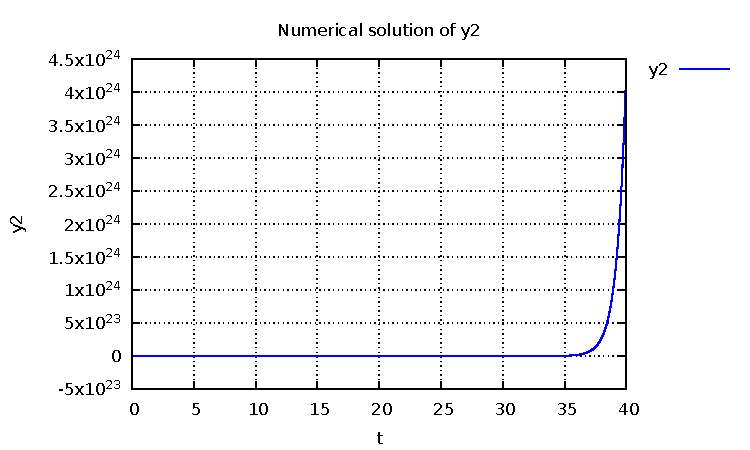
\includegraphics[scale=1.1]{f_2}
\caption{\textsc{Numerical Solution of $y_2$ of Bonus Problem.}}
\end{figure}
\begin{figure}[H]
\centering
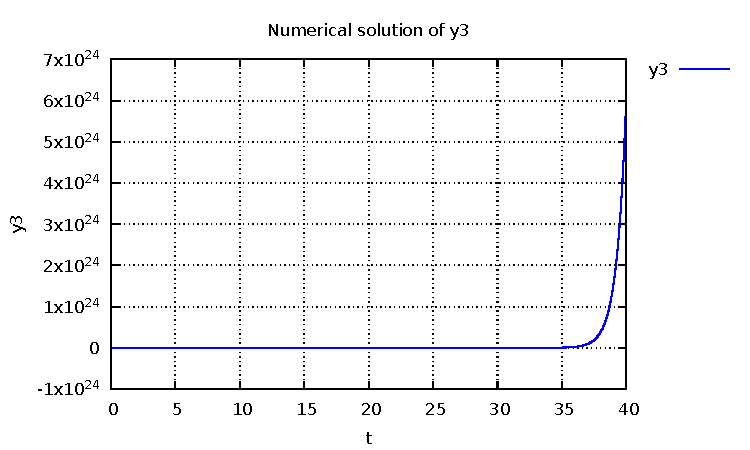
\includegraphics[scale=1.1]{f_3}
\caption{\textsc{Numerical Solution of $y_3$ of Bonus Problem.}}
\end{figure}
\begin{figure}[H]
\centering
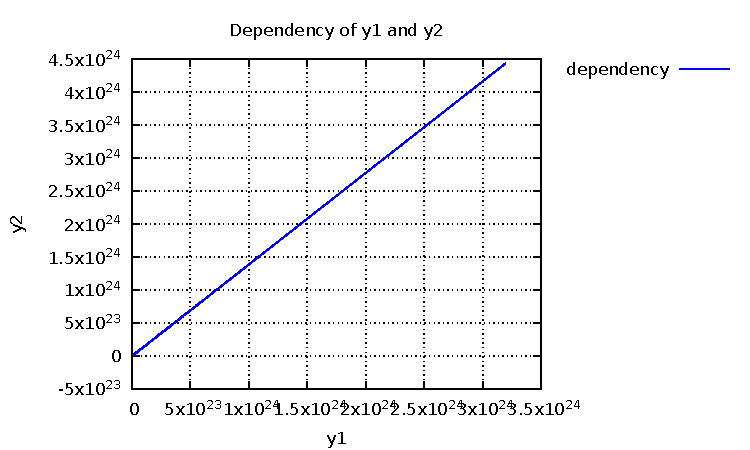
\includegraphics[scale=1.1]{f_d_1_2}
\caption{\textsc{Dependency of $y_1$ and $y_2$ of Bonus Problem.}}
\end{figure}\begin{figure}[H]
\centering
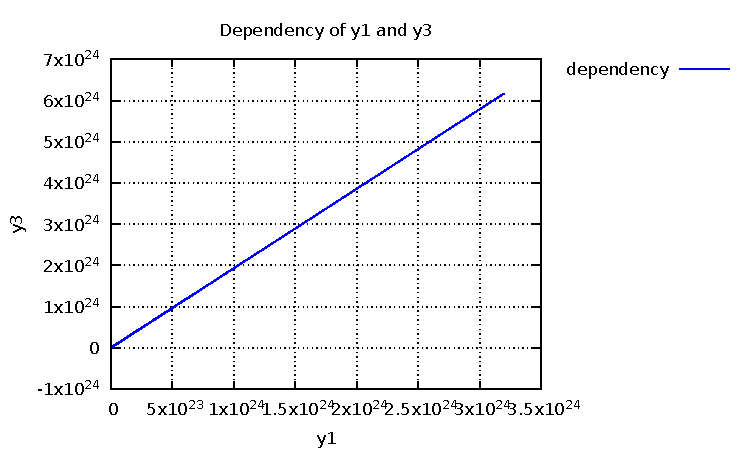
\includegraphics[scale=1.1]{f_d_1_3}
\caption{\textsc{Dependency of $y_1$ and $y_3$ of Bonus Problem.}}
\end{figure}
\begin{figure}[H]
\centering
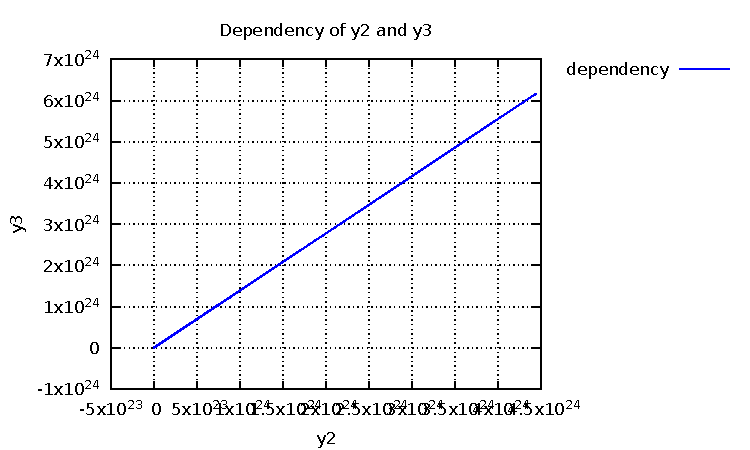
\includegraphics[scale=1.1]{f_d_2_3}
\caption{\textsc{Dependency of $y_2$ and $y_3$ of Bonus Problem.}}
\end{figure}
\begin{figure}[H]
\centering
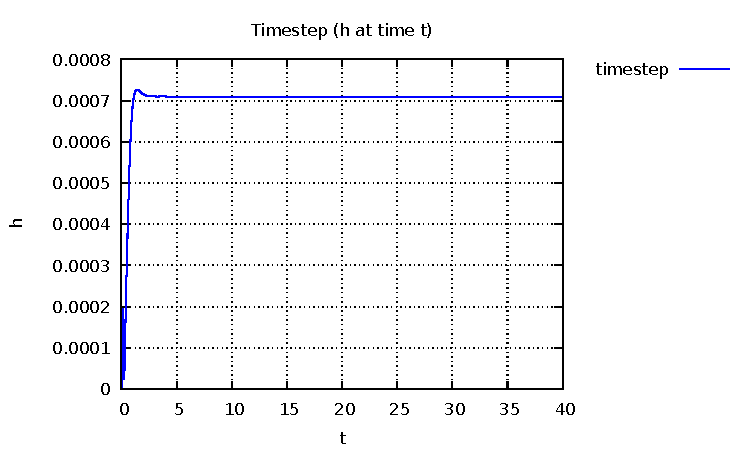
\includegraphics[scale=1.1]{f_ts}
\caption{\textsc{Timestep of Bonus Problem.}}
\end{figure}

\section{Alternative Examples}
We propose this alternative examples ourselves.
\begin{align}
\frac{{d{y_1}}}{{dt}} &= {y_1} - {y_2}\\
\frac{{d{y_2}}}{{dt}} &= 2{y_1} + 4{y_2}
\end{align}
\subsection{Subroutine s2.m}
\begin{verbatim}
function s2 = s2(t)

s2 = [3*exp(2*t)-2*exp(3*t);-3*exp(2*t)+4*exp(3*t)];
\end{verbatim}
\subsection{Subroutine f2.m}
\begin{verbatim}
function f2 = f2(t,y)

% f2=[y(1)-y(2),2*y(1)+4*y(2)];
f2(1) = y(1)-y(2);
f2(2) = 2*y(1)+4*y(2);
\end{verbatim}
\subsection{Subroutine x2.m}
\begin{verbatim}
function x2 = x2(a,b,c,h,t,y)

k1 = f2(t,y);
k2 = f2(t+c(2)*h,y+h*a(2,1)*k1);
k3 = f2(t+c(3)*h,y+h*(a(3,1)*k1+a(3,2)*k2));
k4 = f2(t+c(4)*h,y+h*(a(4,1)*k1+a(4,2)*k2+a(4,3)*k3));
x2  = h*(b(1)*k1+b(2)*k2+b(3)*k3+b(4)*k4);
\end{verbatim}
\subsection{Main Routine RK4ex2.m}
\begin{verbatim}
clear all
close all
clc
format long

tic
% %% Initial for Reference Solutions.
% N0 = 10^6;
% h0= 20/N0;
% t0 = 0:h0:20;
% 
% B1 = zeros(N0,2);
% B1(1,1) = 1;
% B1(1,2) = 1;
% 
% B2 = zeros(N0,2);
% B2(1,1) = 1;
% B2(1,2) = 1;

%% Initial for Numerical Solutions.
N = 10^4;
h = 1/N;
t = 0:h:1;

A1 = zeros(N+1,2);
A1(1,1) = 1;
A1(1,2) = 1;

A2 = zeros(N+1,2);
A2(1,1) = 1;
A2(1,2) = 1;

A3 = zeros(N+1,2);
A3(1,1) = 1;
A3(1,2) = 1;

% Step 
% step = N0/N;

%% Explicit Runge Kutta initials.
% Coefficients
a1 = [0 0 0 0 ;
    1/2 0 0 0 ;
    0 1/2 0 0 ;
    0 0 1 0];
b1 = [1/6 1/3 1/3 1/6];
c1 = [0 1/2 1/2 1];

a2 = [0 0 0 0 ;
    1/3 0 0 0 ;
    -1/3 1 0 0 ;
    1 -1 1 0];
b2 = [1/8 3/8 3/8 1/8];
c2 = [0 1/3 2/3 1];

% %% Reference Solutions.
% for n=1:N0
%     B1(n+1,:) = B1(n,:) + x(a1,b1,c1,h0,t0(n),B1(n,:));
%     B2(n+1,:) = B2(n,:) + x(a2,b2,c2,h0,t0(n),B2(n,:));
% end
s=s2(t)';
%% Numerical Solutions, Absolute Errors and Relative Errors.

ae1 = zeros(N+1,2);
ae2 = zeros(N+1,2);
re1 = zeros(N+1,2);
re2 = zeros(N+1,2);

for n=1:N
%     Numerical Solutions
    A1(n+1,:) = A1(n,:) + x2(a1,b1,c1,h,t(n),A1(n,:));
    A2(n+1,:) = A2(n,:) + x2(a2,b2,c2,h,t(n),A2(n,:));

%     Absolute Errors
%     ae1(n,:) = h.*abs(A1(n,:)-B1(step*(n-1)+1,:));
    ae1 = (abs(A1-s));
%     ae2(n,:) = h.*abs(A2(n,:)-B2(step*(n-1)+1,:));
    ae2 = (abs(A2-s));
%     ae1(n,1) = abs((A1(n,1)-s(1,t));
%     ae1(n,2) = abs((A1(n,2)-s(2,t));
%     ae2(n,1) = abs((A2(n,i)-s(1,t));
%     ae2(n,2) = abs((A2(n,i)-s(2,t));
    
%     Relative Errors
%     re1(n,:) = h.*abs((A1(n,:)-B1(step*(n-1)+1,:))./B1(step*(n-1)+1,:));
    re1 = (abs((A1-s)./s));
%     re2(n,:) = h.*abs((A2(n,:)-B2(step*(n-1)+1,:))./B2(step*(n-1)+1,:));
    re2 = (abs((A2-s)./s));

%     re1(n,1) = abs((A1(n,1)-s(1,t))./s(i,t));
%     re1(n,2) = abs((A1(n,2)-s(2,t))./s(i,t));
%     re2(n,1) = abs((A2(n,i)-s(1,t))./s(i,t));
%     re2(n,2) = abs((A2(n,i)-s(2,t))./s(i,t));

end

% Absolute Errors
display('Absolute Error of Table 1')
ae1_y1 = h*sum(ae1(:,1))
ae1_y2 = h*sum(ae1(:,2))
display('Absolute Error of Table 2')
ae2_y1 = h*sum(ae2(:,1))
ae2_y2 = h*sum(ae2(:,2))

% Relative Errors
display('Relative Error of Table 1')
re1_y1 = h*sum(re1(:,1))
re1_y2 = h*sum(re1(:,2))
display('Relative Error of Table 2')
re2_y1 = h*sum(re2(:,1))
re2_y2 = h*sum(re2(:,2))


%% Plot Numerical Solution

figure(1)   
subplot(2,1,1)
hold on
% plot(t,s(1,t),'b')
plot(t,s(:,1),'b')
plot(t,A1(:,1),'r')
legend('Exact/Reference','Numerical Solution');
title('Numerical Solution for Y1 (Butcher Table 1)');

subplot(2,1,2)
hold on
% plot(t,s(2,t),'b')
plot(t,s(:,2),'b')
plot(t,A1(:,2),'r')
legend('Exact/Reference','Numerical Solution');
title('Numerical Solution for Y2 (Butcher Table 1)');

figure(2)
subplot(2,1,1)
hold on
% plot(t,s(1,t),'b')
plot(t,s(:,1),'b')
plot(t,A2(:,1),'r')
legend('Exact/Reference','Numerical Solution');
title('Numerical Solution for Y1 (Butcher Table 2)');

subplot(2,1,2)
hold on
% plot(t,s(2,t),'b')
plot(t,s(:,2),'b')
plot(t,A2(:,2),'r')
legend('Exact/Reference','Numerical Solution');
title('Numerical Solution for Y2 (Butcher Table 2)');

%% Plot: Dependency of y2 with respect to y1.
figure(3)
hold on
plot(A1(:,1),A1(:,2),'b');
plot(A2(:,1),A2(:,2),'g');
% plot(A3(:,1),A3(:,2),'r');
legend('Butcher Table 1','Butcher Table 2');
title('Dependency of y2 with respect to y1');

%% Plot Absolute Errors.
figure(4)
subplot(2,1,1)
hold on
plot(t,ae1(:,1),'b');
plot(t,ae2(:,1),'g');
% plot(t,ae3(:,1),'r');
legend('Butcher Table 1','Butcher Table 2');
title('Absolute Errors Y1');

subplot(2,1,2)
hold on
plot(t,ae1(:,2),'b');
plot(t,ae2(:,2),'g');
% plot(t,ae3(:,2),'r');
legend('Butcher Table 1','Butcher Table 2');
title('Absolute Errors Y2');

%% Plot Relative Errors.
figure(5)
subplot(2,1,1)
hold on
plot(t,re1(:,1),'b');
plot(t,re2(:,1),'g');
% plot(t,re3(:,1),'r');
legend('Butcher Table 1','Butcher Table 2');
title('Relative Errors Y1');

subplot(2,1,2)
hold on
plot(t,re1(:,2),'b');
plot(t,re2(:,2),'g');
% plot(t,re3(:,2),'r');
legend('Butcher Table 1','Butcher Table 2');
title('Relative Errors Y2');

toc
\end{verbatim}

\subsection{Results}
\begin{figure}[H]
\centering
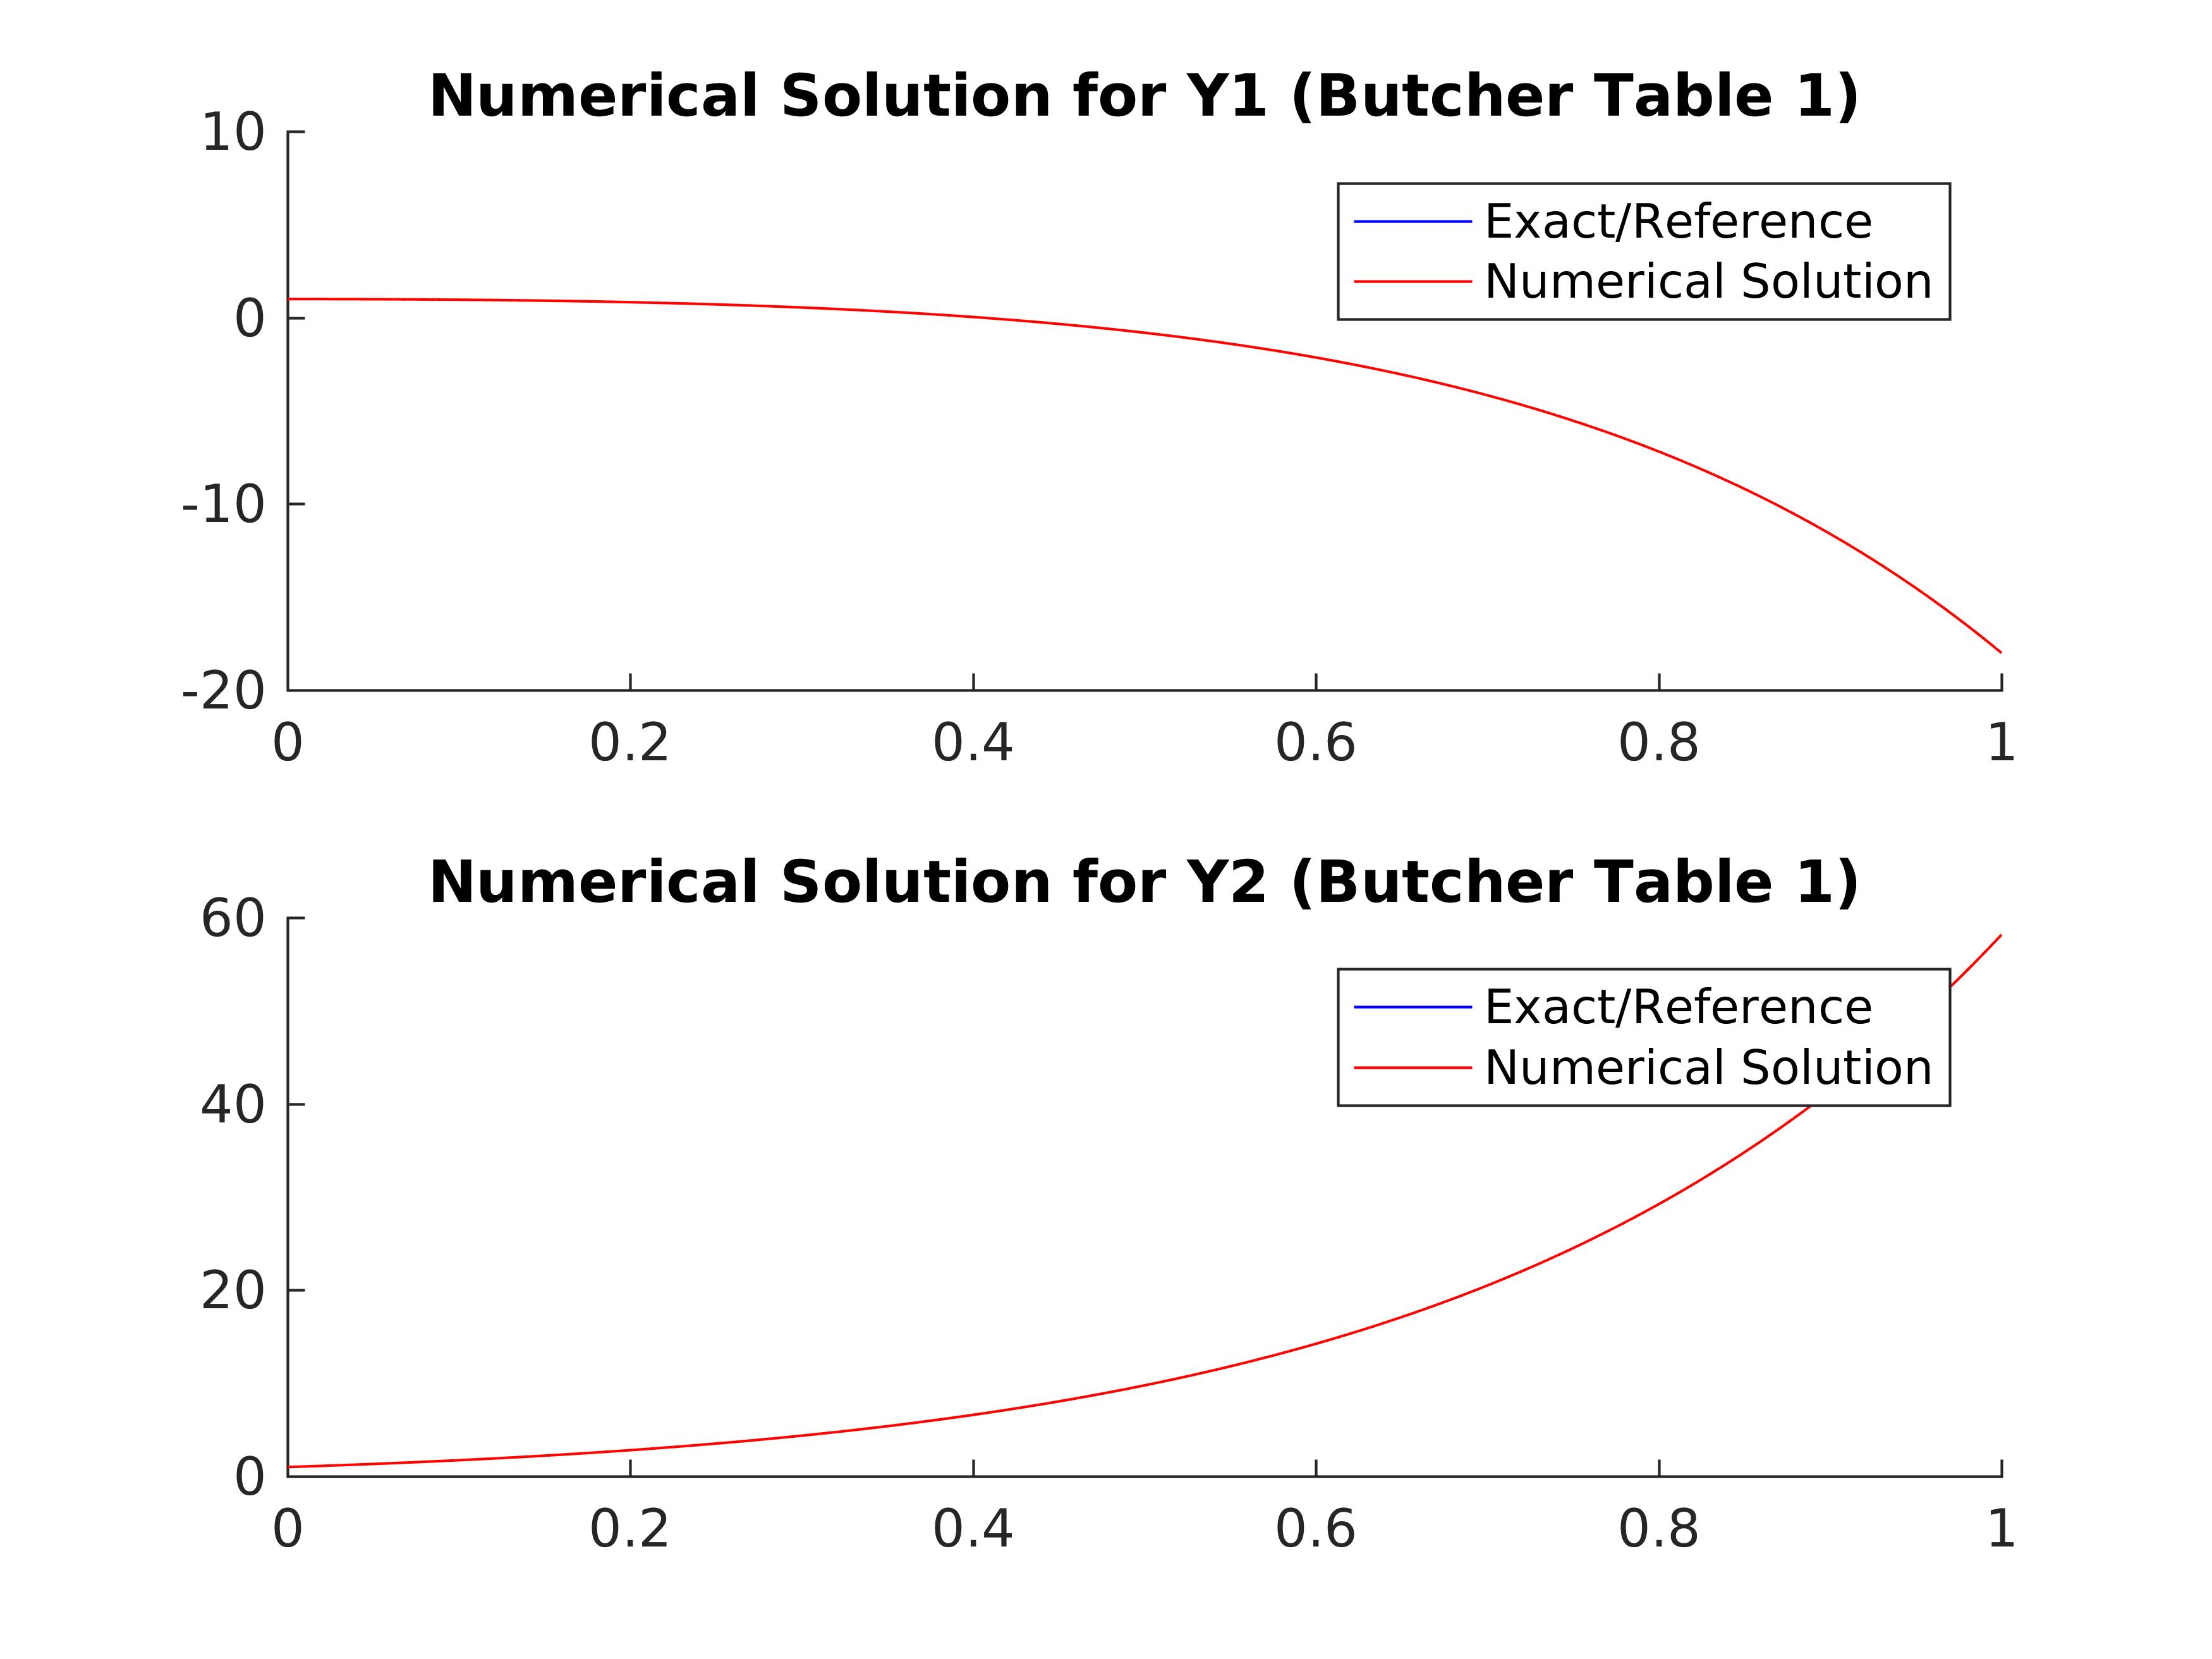
\includegraphics[scale=0.09]{3ns1}
\caption{\textsc{Numerical Solutions of Alternative Example.}}
\end{figure}
\begin{figure}[H]
\centering
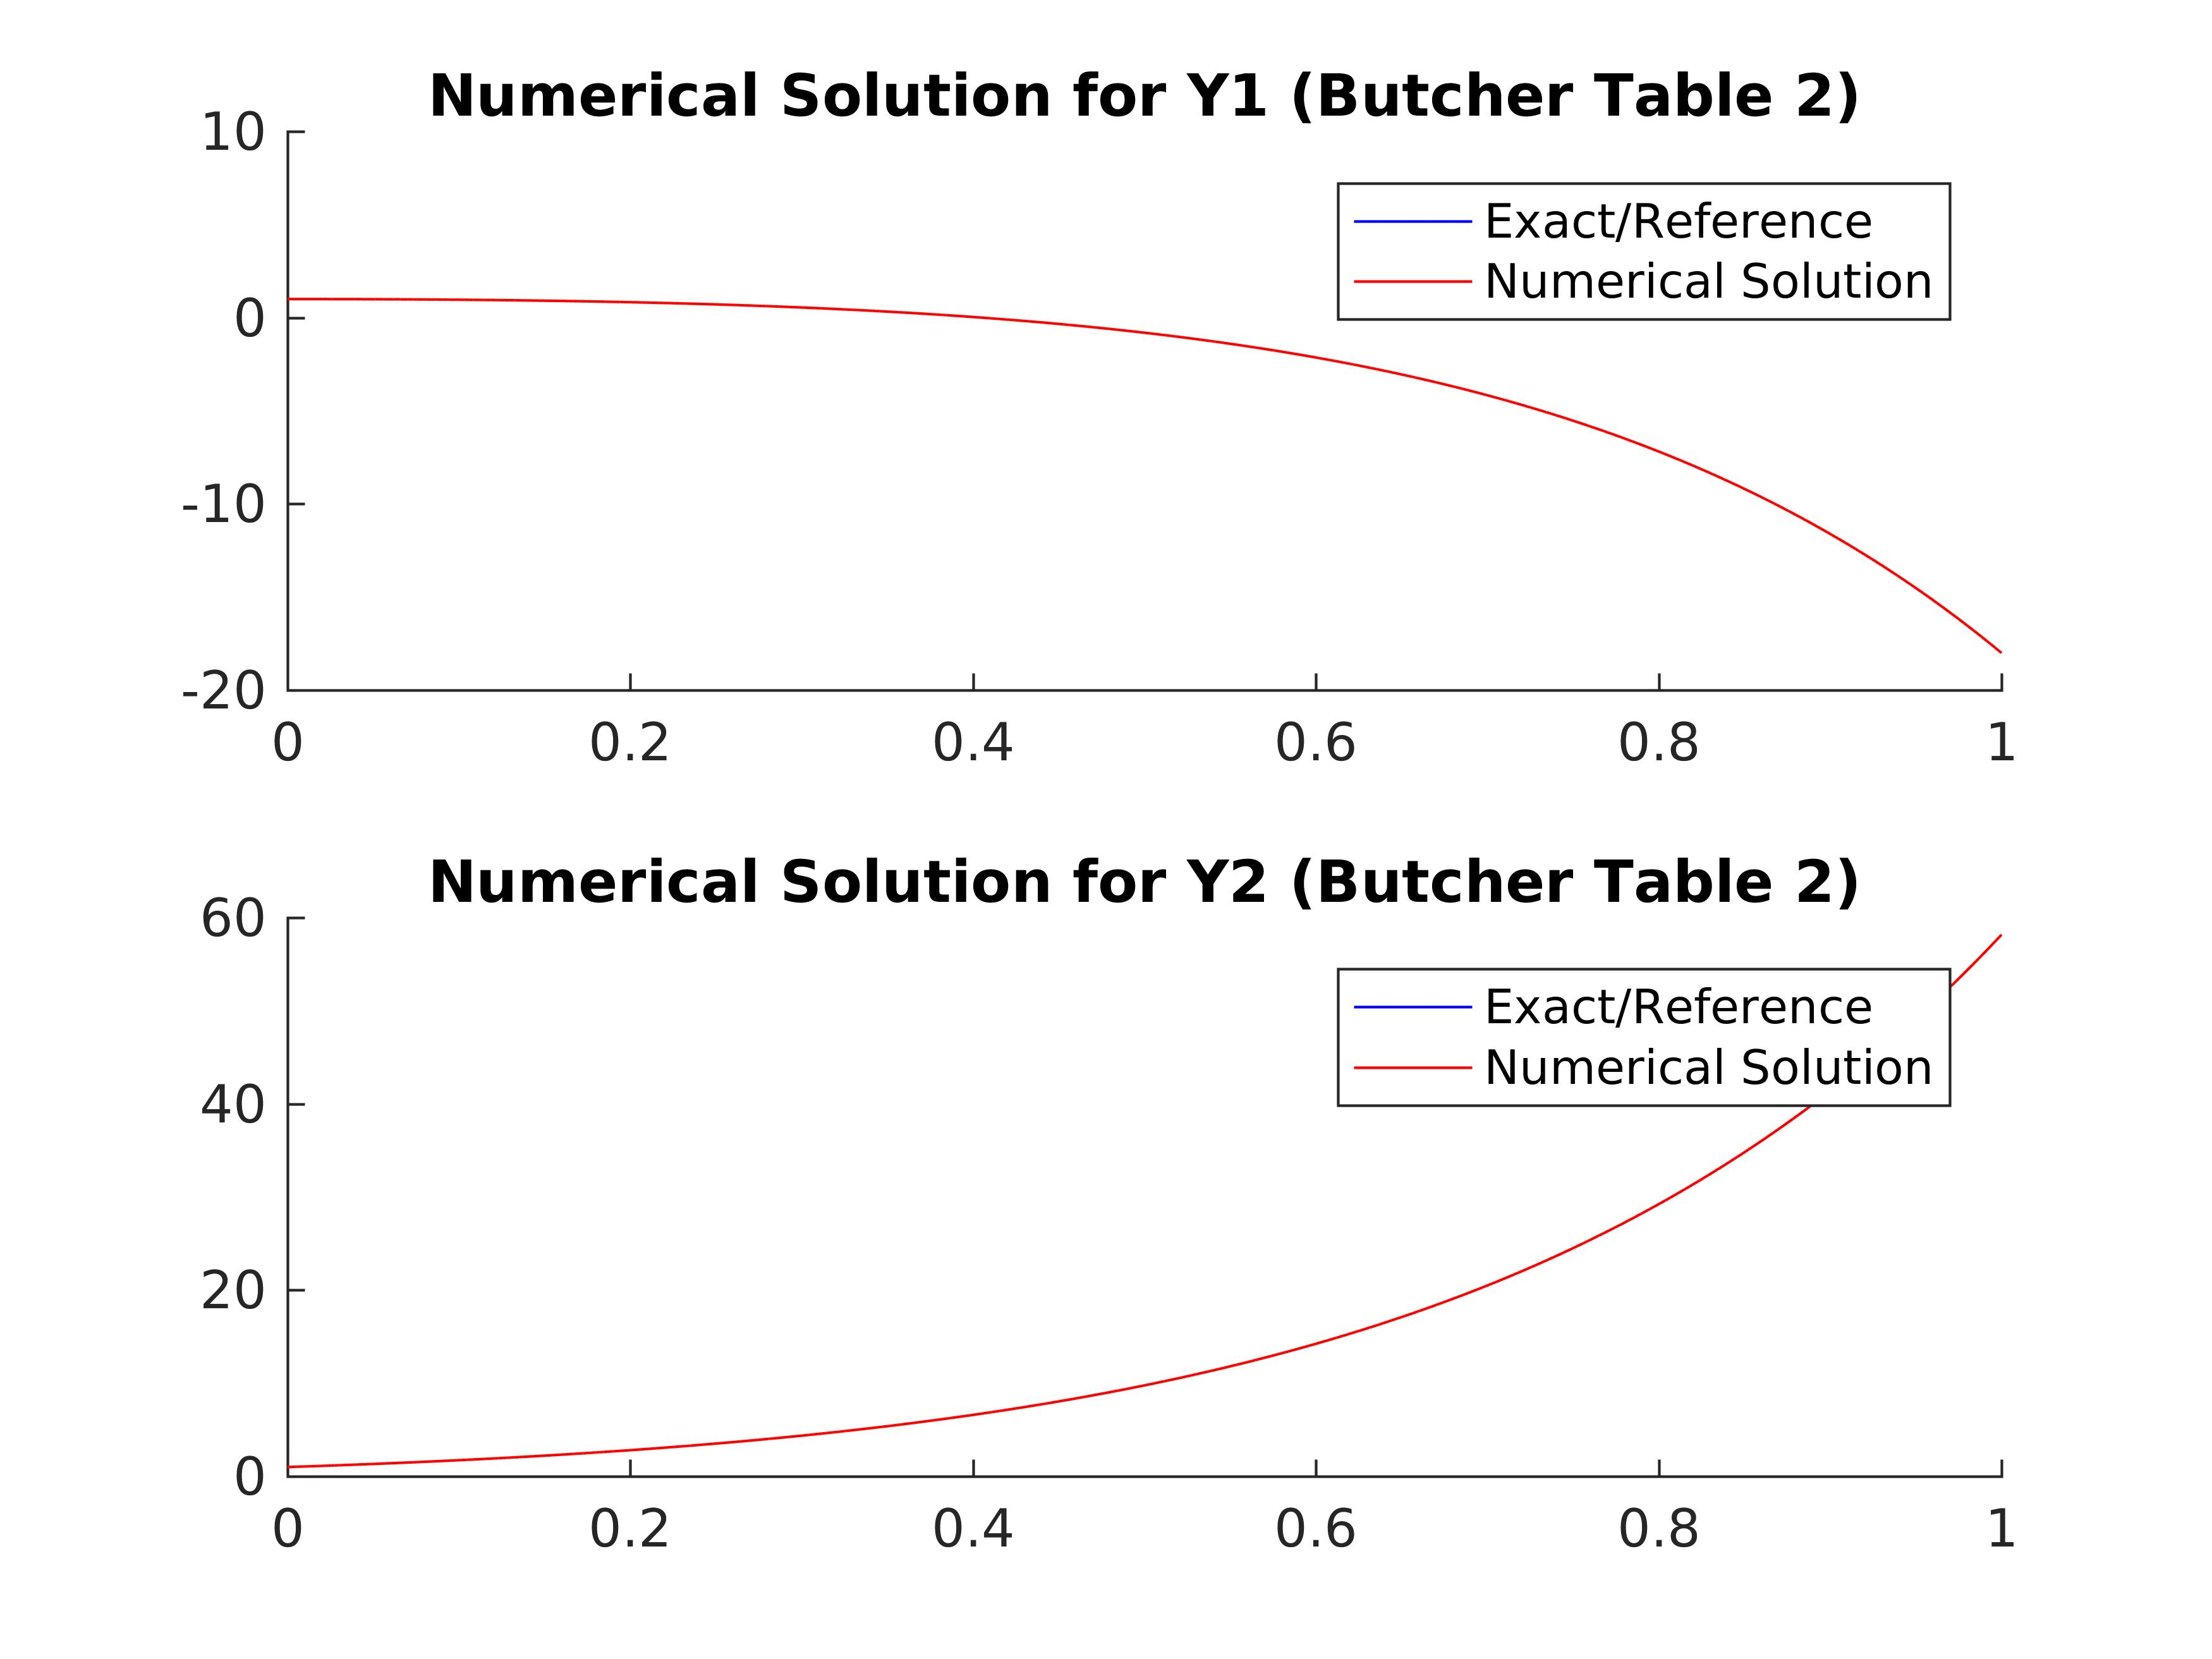
\includegraphics[scale=0.09]{3ns2}
\caption{\textsc{Numerical Solutions of Alternative Example.}}
\end{figure}
\begin{figure}[H]
\centering
\includegraphics[scale=0.09]{3d}
\caption{\textsc{Dependency of $y_2$ with respect to $y_1$ of Alternative Example.}}
\end{figure}
\begin{figure}[H]
\centering
\includegraphics[scale=0.09]{3ae}
\caption{\textsc{Absolute Errors of Alternative Example.}}
\end{figure}
\begin{figure}[H]
\centering
\includegraphics[scale=0.09]{3re}
\caption{\textsc{Relative Errors of Alternative Example.}}
\end{figure}

\section{\textsc{Fortran} Codes}
See attached user guide to use these codes.
\begin{lstlisting}
program rkats
	use customf ! module for systems of ODEs
	implicit none
    ! error tolerance
	real (kind = 8) :: h=1d-5,htol=1d-9,at=1d-4,rt=1d-3 
	real (kind = 8) :: fac=0.9d0,facmin=0.5d0,facmax=2d0
	real (kind = 8) :: s,er,start,finish
	integer :: i,j=1,p=2,v1,v2,inputerror
	real (kind = 8), dimension(dms) :: r2,r3,x2,x3,e
	real (kind = 8), dimension(4,4) :: a2,a3
	real (kind = 8), dimension(4) :: b2,b3,c2,c3
	
	call cpu_time(start)
	a2=reshape((/0.0,0.0,0.0,0.0,&
		1.0,0.0,0.0,0.0,&
		0.0,0.0,0.0,0.0,&
		0.0,0.0,0.0,0.0/)&
		,shape(a2),order=(/2,1/))
	b2=(/0.5,0.5,0.0,0.0/)
	c2=(/0.0,1.0,0.0,0.0/)

	a3=reshape((/0.0,0.0,0.0,0.0,&
		1.0,0.0,0.0,0.0,&
		0.25,0.25,0.0,0.0,&
		0.0,0.0,0.0,0.0/)&
		,shape(a3),order=(/2,1/))
	b3=(/1/6d0,1/6d0,2/3d0,0d0/)
	c3=(/0.0,1.0,0.5,0.0/)

	open(unit=1,file="data.txt",form="formatted", &
	     status="replace",action="write")
	do while (t<=te)
		call rk(a2,b2,c2,a3,b3,c3,h,t,x,x2,x3)
		r2=x+x2
		r3=x+x3
		s=0d0
		do i=1,dms
			s=s+((r2(i)-r3(i))/(at+max(abs(r2(i)),abs(r3(i)))*rt))**2
		end do
		er=sqrt(s/d)
		if (er>1d0) then
			facmax=1d0
			h=h*min(facmax,max(facmin,fac/(er**(1/4d0))))
			if (h<=htol) then
				print *, 'stop'
				stop
			else 
				cycle
			end if
		end if
		write(1,*) t,h,(x(i), i=1,dms)
		x=r3
		t=t+h
		facmax=2d0
		h=h*min(facmax,max(facmin,fac/(er**(1/4d0))))
	end do
	!write(1,*) t,h,(x(i), i=1,dms)
	close(unit=1)
	call cpu_time(finish)
	write(*,*) 'Finished',finish-start
	
	open(unit=2,file="para1.plt",form="formatted", &
	     status='replace',action="readwrite")
		write(2,"(a,i0)") "d=",dms
		write(2,"(a,i0)") "p=",p
	close(unit=2)
	call system('gnuplot data_plot.plt')
	
	if (dms>=2) then
		do while (j/=0)
			write(*,*) 'Do you want to plot the dependency &
 of 2 solutions ?'
			write(*,*) 'Enter 1 for "Yes" and 0 for "No".'
			read (*,"(i10)",iostat=inputerror) j
			if (j/=0 .and. j/=1 .or. inputerror/=0) then
				write(*,*) 'Invalid input ! Input must be either 1 or 0'
				cycle
			end if
			if (j==1) then
				write(*,*) 'Which of the 2 solutions you &
want to plot dependency ?'
				write(*,"(a,i0,a)") 'Enter the integer &
 corresponding to the first solution (from 1 to ',dms,') &
 to plot dependency'
				read (*,"(i10)",iostat=inputerror) v1
				if (v1<1 .or. v1>dms .or. inputerror/=0) then
					write(*,"(a,i0,a)") 'Invalid input ! Input must be &
 a integer from 1 to ',dms,'.'
					cycle
				end if
				write(*,"(a,i0,a)") 'Enter the integer corresponding to &
 the second solution (from 1 to ',dms,') to plot dependency'
				read (*,"(i10)",iostat=inputerror) v2
				if (v2<1 .or. v2>dms .or. inputerror/=0) then
					write(*,"(a,i0,a)") 'Invalid input ! Input must be &
 a integer from 1 to ',dms,'.'
					cycle
				else if (v2==v1) then
					write(*,*) 'Invalid input ! The second input must be & 
 a different from the first input.'
					cycle
				end if
				open(unit=3,file="para2.plt",form="formatted", &
 status='replace',action="readwrite")
					write(3,"(a,i0)") "v1=",v1
					write(3,"(a,i0)") "v2=",v2
				close(unit=3)
				call system('gnuplot data_plot_dependency.plt')
			end if
		end do
	end if
	
contains
	subroutine rk(a1,b1,c1,a2,b2,c2,h,t,x,x1,x2)
		implicit none
		real (kind = 8), intent(in) :: t,h
		real (kind = 8), dimension(dms), intent(in) :: x
		real (kind = 8), dimension(4,4), intent(in) :: a1, a2
		real (kind = 8), dimension(4), intent(in) :: b1, c1, b2, c2
		real (kind = 8), dimension(dms), intent(out) :: x1, x2
		real (kind = 8), dimension(dms) :: k1,k2,k3,k4
		
		call f(t,x,k1)
		call f(t+c1(2)*h, x+h*a1(2,1)*k1, k2)
		call f(t+c1(3)*h, x+h*(a1(3,1)*k1+a1(3,2)*k2), k3)
		call f(t+c1(4)*h, x+h*(a1(4,1)*k1+a1(4,2)*k2+a1(4,3)*k3), k4)
		x1 = h*(b1(1)*k1+b1(2)*k2+b2(3)*k3+b1(4)*k4);

		call f(t+c2(2)*h, x+h*a2(2,1)*k1, k2)
		call f(t+c2(3)*h, x+h*(a2(3,1)*k1+a2(3,2)*k2), k3)
		call f(t+c2(4)*h, x+h*(a2(4,1)*k1+a2(4,2)*k2+a2(4,3)*k3), k4)
		x2 = h*(b2(1)*k1+b2(2)*k2+b2(3)*k3+b2(4)*k4);
	end subroutine rk
	
end program rkats
\end{lstlisting}

\begin{lstlisting}
program rkfts
	use customf ! module for systems of ODEs
	implicit none
	real (kind = 8) :: h=1d-2 ! time step
	real (kind = 8) :: start,finish
	integer :: i,j=1,p=1,v1,v2,inputerror
	real (kind = 8), dimension(dms) :: r
	real (kind = 8), dimension(4,4) :: a
	real (kind = 8), dimension(4) :: b,c

	call cpu_time(start)
	a=reshape((/0d0,0d0,0d0,0d0,&
		1/2d0,0d0,0d0,0d0,&
		0d0,1/2d0,0d0,0d0,&
		0d0,0d0,1d0,0d0/)&
		,shape(a),order=(/2,1/))
	b=(/1/6d0,1/6d0,2/3d0,0d0/)
	c=(/0d0,1/2d0,1/2d0,1d0/)

	open(unit=1,file="data.txt",form="formatted",status="replace",&
 action="write")
	do while (t<=te)
		write(1,*) t,(x(i), i=1,dms)
		call rk(a,b,c,h,t,x,r)
		x=x+r
		t=t+h
	end do
	!write(1,*) t,(x(i), i=1,dms)
	close(unit=1)
	call cpu_time(finish)
	write(*,*) 'Finished',finish-start

	open(unit=2,file="para1.plt",form="formatted",status='replace', &
 action="readwrite")
		write(2,"(a,i0)") "d=",dms
		write(2,"(a,i0)") "p=",p
	close(unit=2)
	call system('gnuplot data_plot.plt')
	
	if (dms>=2) then
		do while (j/=0)
			write(*,*) 'Do you want to plot the dependency of 2 solutions ?'
			write(*,*) 'Enter 1 for "Yes" and 0 for "No".'
			read (*,"(i10)",iostat=inputerror) j
			if (j/=0 .and. j/=1 .or. inputerror/=0) then
				write(*,*) 'Invalid input ! Input must be either 1 or 0'
				cycle
			end if
			if (j==1) then
				write(*,*) 'Which of the 2 solutions you want &
 to plot dependency ?'
				write(*,"(a,i0,a)") 'Enter the integer corresponding to &
 the first solution (from 1 to ',dms,') to plot dependency'
				read (*,"(i10)",iostat=inputerror) v1
				if (v1<1 .or. v1>dms .or. inputerror/=0) then
					write(*,"(a,i0,a)") 'Invalid input ! Input must be &
 a integer from 1 to ',dms,'.'
					cycle
				end if
				write(*,"(a,i0,a)") 'Enter the integer corresponding to &
 the second solution (from 1 to ',dms,') to plot dependency'
				read (*,"(i10)",iostat=inputerror) v2
				if (v2<1 .or. v2>dms .or. inputerror/=0) then
					write(*,"(a,i0,a)") 'Invalid input ! Input must be &
 a integer from 1 to ',dms,'.'
					cycle
				else if (v2==v1) then
					write(*,*) 'Invalid input ! The second input must be &
 a different from the first input.'
					cycle
				end if
				open(unit=3,file="para2.plt",form="formatted", & 
 status='replace',action="readwrite")
					write(3,"(a,i0)") "v1=",v1
					write(3,"(a,i0)") "v2=",v2
				close(unit=3)
				call system('gnuplot data_plot_dependency.plt')
			end if
		end do
	end if

contains
	subroutine rk(a,b,c,h,t,x,r)
		implicit none
		real (kind = 8), intent(in) :: t,h
		real (kind = 8), dimension(dms), intent(in) :: x
		real (kind = 8), dimension(4,4), intent(in) :: a
		real (kind = 8), dimension(4), intent(in) :: b, c
		real (kind = 8), dimension(dms), intent(out) :: r
		real (kind = 8), dimension(dms) :: k1,k2,k3,k4
		
		call f(t,x,k1)
		call f(t+c(2)*h, x+h*a(2,1)*k1, k2)
		call f(t+c(3)*h, x+h*(a(3,1)*k1+a(3,2)*k2), k3)
		call f(t+c(4)*h, x+h*(a(4,1)*k1+a(4,2)*k2+a(4,3)*k3), k4)
		r = h*(b(1)*k1+b(2)*k2+b(3)*k3+b(4)*k4);
	end subroutine rk
	
end program rkfts
\end{lstlisting}

\begin{lstlisting}
load 'para1.plt'

font=20
set key outside right
set grid
data='./data.txt'

if (p==2) {
set terminal push
set terminal lua tikz fulldoc createstyle
outfiletex = 'fig_ts.tex'
set output outfiletex
set title 'Timestep (h at time t)'
set xlabel 't'
set ylabel 'h'
plot data using 1:2 with lines title 'timestep' lt rgb 'blue'

set terminal pdf
outfilepdf = 'fig_ts.pdf'
set output  outfilepdf
replot

set terminal wxt 1 persist
set output
replot
}

do for [i=1:d] {
j=i+p-1
k=i+p
set terminal push
set terminal lua tikz fulldoc createstyle
outfiletex = 'fig_'.i.'.tex'
set output outfiletex
set xlabel 't'
set ylabel 'y'.i
set title 'Numerical solution of y'.i
plot data using 1:k with lines title 'y'.i lt rgb 'blue'

set terminal pdf
outfilepdf = 'fig_'.i.'.pdf'
set output  outfilepdf
replot

set terminal wxt j persist
set output 
replot
}
\end{lstlisting}

\begin{lstlisting}
load 'para1.plt'
load 'para2.plt'

font=20
set key outside right
set grid
data='./data.txt'

f1=v1+p
f2=v2+p
set terminal push
set terminal lua tikz fulldoc createstyle
outfiletex = 'fig_d_'.v1.'_'.v2.'.tex'
set output outfiletex
set xlabel 'y'.v1
set ylabel 'y'.v2
set title 'Dependency of y'.v1.' and y'.v2
plot data using f1:f2 with lines title 'dependency' lt rgb 'blue'

set terminal pdf
outfilepdf = 'fig_d_'.v1.'_'.v2.'.pdf'
set output  outfilepdf
replot

e=d+p
set terminal wxt e persist
set output
replot
\end{lstlisting}

\begin{lstlisting}
module ch  
implicit none 
	integer, parameter :: dms=1 ! number of unknowns
    ! initial condition
	real (kind = 8), dimension(dms) :: x=(/1d0/) 
    ! begining time and ending time
	real (kind = 8) :: t=0d0,te=40d0 
	real (kind = 8) :: d=real(dms)
contains      
	subroutine f(t,y,f0)
		implicit none
		real (kind = 8), intent(in) :: t
		real (kind = 8), dimension(dms), intent(in) :: y
		real (kind = 8), dimension(dms), intent(out) :: f0
		
		f0(1)=-50*(y(1)-cos(t))
	end subroutine f
end module ch 
\end{lstlisting}

\begin{lstlisting}
module b  
implicit none 
	integer, parameter :: dms=2 ! number of unknowns
    ! initial condition
	real (kind = 8), dimension(dms) :: x=(/1d0, 1d0/) 
    ! begining time and ending time
	real (kind = 8) :: t=0d0,te=40d0 
	real (kind = 8) :: d=real(dms)
contains      
	subroutine f(t,y,f0)
		implicit none
		real (kind = 8), intent(in) :: t
		real (kind = 8), dimension(dms), intent(in) :: y
		real (kind = 8), dimension(dms), intent(out) :: f0
		
		f0(1)=1d0-4d0*y(1)+y(2)*(y(1)**2)
		f0(2)=3d0*y(1)-y(2)*(y(1)**2)
	end subroutine f
end module b 
\end{lstlisting}

\begin{lstlisting}
module bz2  
implicit none 
	integer, parameter :: dms=2 ! number of unknowns
    ! initial condition
	real (kind = 8), dimension(dms) :: x=(/1d-5, 1d-5/) 
    ! begining time and ending time
	real (kind = 8) :: t=0d0,te=40d0 
	real (kind = 8) :: d=real(dms)
contains      
	subroutine f(t,y,f0)
		implicit none
		real (kind = 8), intent(in) :: t
		real (kind = 8), dimension(dms), intent(in) :: y
		real (kind = 8), dimension(dms), intent(out) :: f0
		
		f0(1)=(y(1)*(1-y(1))+2/3d0*y(2)*(8d-4-y(1))/(8d-4+y(1)))*0.25d+2
		f0(2)=y(1)-y(2)
	end subroutine f
end module bz2
\end{lstlisting}

\begin{lstlisting}
module bz3
implicit none 
	integer, parameter :: dms=3 ! number of unknowns
    ! initial condition	
	real (kind = 8), dimension(dms) :: x=(/1d-5, 1d-5, 1d-5/) 
    ! begining time and ending time
	real (kind = 8) :: t=0d0,te=40d0 
	real (kind = 8) :: d=real(dms)
contains      
	subroutine f(t,y,f0)
		implicit none
		real (kind = 8), intent(in) :: t
		real (kind = 8), dimension(dms), intent(in) :: y
		real (kind = 8), dimension(dms), intent(out) :: f0
		
		f0(1)=(4d-4*y(2)-y(1)*y(2)+y(1)*(1-y(1)))*0.25d+2
		f0(2)=(-4d-4*y(2)-y(1)*y(2)+(2/3d0)*y(3))*0.25d+4
		f0(3)=y(1)-y(3)
	end subroutine f
end module bz3
\end{lstlisting}

\begin{lstlisting}
module o  
implicit none 
	integer, parameter :: dms=3 ! number of unknowns
    ! initial condition	
	real (kind = 8), dimension(dms) :: x=(/1d0, 2d0, 3d0/) 
    ! begining time and ending time
	real (kind = 8) :: t=0d0,te=1200d0 
	real (kind = 8) :: d=real(dms)
contains      
	subroutine f(t,y,f0)
		implicit none
		real (kind = 8), intent(in) :: t
		real (kind = 8), dimension(dms), intent(in) :: y
		real (kind = 8), dimension(dms), intent(out) :: f0
		
		f0(1)=77.27d0*(y(2)+y(1)*(1-8.375d-6*y(1)-y(2)))
		f0(2)=(y(3)-(1+y(1))*y(2))/77.27d0
		f0(3)=0.161d0*(y(1)-y(3))
	end subroutine f
end module o 
\end{lstlisting}

\begin{lstlisting}
module vdp  
implicit none 
	integer, parameter :: dms=2 ! number of unknowns
    ! initial condition	
	real (kind = 8), dimension(dms) :: x=(/2d0, -0.66d0/) 
    ! begining time and ending time	
	real (kind = 8) :: t=0d0,te=2d0 
	real (kind = 8) :: d=real(dms)
contains      
	subroutine f(t,y,f0)
		implicit none
		real (kind = 8), intent(in) :: t
		real (kind = 8), dimension(dms), intent(in) :: y
		real (kind = 8), dimension(dms), intent(out) :: f0
		
		f0(1)=y(2)
		f0(2)=(((1-(y(1)**2))*y(2))-y(1))*1d+6
	end subroutine f
end module vdp 
\end{lstlisting}

\begin{lstlisting}
module customf
implicit none 
	integer, parameter :: dms=3 ! number of unknowns
    ! initial condition	
	real (kind = 8), dimension(dms) :: x=(/6d0, -1d0, -1d0/) 
    ! begining time and ending time
	real (kind = 8) :: t=0d0,te=40d0 
	real (kind = 8) :: d=real(dms)
contains      
	subroutine f(t,y,f0)
		implicit none
		real (kind = 8), intent(in) :: t
		real (kind = 8), dimension(dms), intent(in) :: y
		real (kind = 8), dimension(dms), intent(out) :: f0
		
		f0(1)=y(2)
		f0(2)=y(3)
		f0(3)=6*y(1)-y(2)-y(3)
	end subroutine f
end module customf
\end{lstlisting}
\part{Implicit Runge Kutta Methods}
\chapter{Introduction to Implicit Runge Kutta Methods}
Explicit Runge Kutta methods are generally unsuitable for the solution of stiff equations\index{stiff equations} because their region of absolute stability\index{region of absolute stability} is small. In particular, is is bounded. This issue is especially important in the solution of partial differential equations\index{solution of partial differential equations}.
\section{General Implicit Runge Kutta Method}
The instability of explicit Runge Kutta methods\index{instability of explicit Runge Kutta methods} motivates the development of implicit methods\index{implicit methods}.

An implicit Runge Kutta method\index{implicit Runge Kutta method} has the form
\begin{align}
\label{6.1}
{{y_{n + 1}}} = {{y_n}} + h\sum\limits_{i = 1}^s {{b_i}{k_i}} 
\end{align}
where 
\begin{align}
\label{6.2}
{k_i} = f\left( {{\tau _i},{\eta _i}} \right),i = 1,2, \ldots ,s
\end{align}
with 
\begin{align}
{\tau _i} &= {t_n} + {c_i}h\\
{\eta _i} &= {y_n} + h\sum\limits_{j = 1}^s {{a_{ij}}{k_j}} 
\end{align}

The difference with an explicit method is that in an explicit method, the sum over $j$ only goes up to $i-1$. This also shows up in the Butcher tableau: the coefficient matrix\index{coefficient matrix} $a_{ij}$ of an explicit method is lower triangular. In an implicit method\index{implicit method}, the sum over $j$ goes up to $s$ and the coefficient matrix is not triangular, yielding a Butcher tableau\index{Butcher tableau} of the form
\begin{align}
\label{6.3}
\begin{array}{*{20}{c}}
{{c_1}}&\vline& {{a_{11}}}&{{a_{12}}}& \cdots &{{a_{1s}}}\\
{{c_2}}&\vline& {{a_{21}}}&{{a_{22}}}& \cdots &{{a_{2s}}}\\
 \vdots &\vline&  \vdots & \vdots & \ddots & \vdots \\
{{c_s}}&\vline& {{a_{s1}}}&{{a_{s2}}}& \cdots &{{a_{ss}}}\\
\hline
{}&\vline& {{b_1}}&{{b_2}}& \cdots &{{b_s}}\\
{}&\vline& {b_1^*}&{b_2^*}& \cdots &{b_s^*}
\end{array} = \begin{array}{*{20}{c}}
c&\vline& A\\
\hline
{}&\vline& {{b^T}}
\end{array}
\end{align}

The consequence of this difference is that at every step, a system of algebraic equations has to be solved. This increases the computational cost\index{computational cost} considerably. If a method with $s$ stages is used to solve a differential equations with $m$ components, then the system of algebraic equations\index{system of algebraic equations} has $ms$ components. This can be contrasted with \textit{implicit linear multistep methods}\index{implicit linear multistep methods} (the other big family of methods for ODEs): an implicit $s$-step linear multistep method\index{implicit $s$-step linear multistep method} needs to solve a system of algebraic equations with only $m$ components, so the size of the system does not increase as the number of steps increases.
\section{Implicit Runge Kutta First Order Method}
We consider the implicit Runge Kutta first order method\index{implicit Runge Kutta first order method} here because it is very short and easy. There is no need to represent it into a separated chapter.

For $s=1$, \eqref{6.2} becomes
\begin{align}
{k_1} &= f\left( {{t_n} + {c_1}h,{y_n} + h{a_{11}}{k_1}} \right)\\
& = {f_n} + {c_1}h{f_t} + h{a_{11}}{k_1}{f_y} + O\left( {{h^2}} \right)\\
 &= {f_n} + {c_1}h{f_t} + h{a_{11}}\left( {{f_n} + O\left( h \right)} \right){f_y} + O\left( {{h^2}} \right)\\
& = {f_n} + {c_1}h{f_t} + h{a_{11}}{f_n}{f_y} + O\left( {{h^2}} \right)
\end{align}
and \eqref{6.3} becomes
\begin{align}
{{y_{n + 1}}} &= {{y_n}} + h{b_1}{k_1}\\
& = {{y_n}} + h{b_1}\left( {{f_n} + {c_1}h{f_t} + h{a_{11}}{f_n}{f_y} + O\left( {{h^2}} \right)} \right)\\
& = {{y_n}} + h{b_1}{f_n} + {h^2}{b_1}{c_1}{f_t} + {h^2}{a_{11}}{b_1}{f_n}{f_y} + O\left( {{h^3}} \right)
\label{6.12}
\end{align}

We recall \eqref{2.17}
\begin{align}
\label{6.13}
{{y_{n + 1}}} = {{y_n}} + h{f_n} + \dfrac{{{h^2}}}{2}{f_t} + \dfrac{{{h^2}}}{2}{f_n}{f_y} + O\left( {{h^3}} \right) 
\end{align}

Comparing \eqref{6.12} and \eqref{6.13}, we easily obtain
\begin{align}
h{f_n}:{b_1} &= 1\\
{h^2}{f_t}:{b_1}{c_1} &= \dfrac{1}{2}\\
{h^2}{f_n}{f_y}:{b_1}{a_{11}} &= \dfrac{1}{2}
\end{align}
i.e, a system of equations
\begin{align}
{b_1} &= 1\\
{b_1}{c_1} &= \dfrac{1}{2}\\
{b_1}{a_{11}} &= \dfrac{1}{2}
\end{align}

We immediately find out
\begin{align}
{b_1} &= 1\\
{c_1} &= \dfrac{1}{2}\\
{a_{11}} &= \dfrac{1}{2}
\end{align}

Hence, the Butcher table\index{Butcher table} in this case has the following form
\begin{align}
\begin{array}{*{20}{c}}
{\dfrac{1}{2}}&\vline& {\dfrac{1}{2}}\\
\hline
{}&\vline& 1
\end{array}
\end{align}
Done. \hfill $\square$








\chapter{Implicit Runge Kutta Second Order Method}
\section{Derivation of Implicit Runge Kutta Second Order Method}
\subsection{Implicit Runge Kutta Second Order Formula}
\index{implicit Runge Kutta second order method}For $s=2$, \eqref{6.2} becomes
\begin{align}
{k_1} &= f\left( {{t_n} + {c_1}h,{y_n} + h{a_{11}}{k_1} + h{a_{12}}{k_2}} \right)\\
& = {f_n} + {c_1}h{f_t} + h\left( {{a_{11}}{k_1} + {a_{12}}{k_2}} \right){f_y} + \dfrac{1}{2}c_1^2{h^2}{f_{tt}}\\
& + {c_1}{h^2}\left( {{a_{11}}{k_1} + {a_{12}}{k_2}} \right){f_{ty}} + \dfrac{1}{2}{h^2}{\left( {{a_{11}}{k_1} + {a_{12}}{k_2}} \right)^2}{f_{yy}} + O\left( {{h^3}} \right)\\
& = {f_n} + {c_1}h{f_t} + h{a_{11}}\left( {{f_n} + {c_1}h{f_t} + h\left( {{a_{11}} + {a_{12}}} \right){f_n}{f_y}} \right){f_y}\\
& + h{a_{12}}\left( {{f_n} + {c_2}h{f_t} + h\left( {{a_{21}} + {a_{22}}} \right){f_n}{f_y}} \right){f_y} + \dfrac{1}{2}c_1^2{h^2}{f_{tt}}\\
& + {c_1}{h^2}\left( {{a_{11}} + {a_{12}}} \right){f_n}{f_{ty}} + \dfrac{1}{2}{h^2}{\left( {{a_{11}} + {a_{12}}} \right)^2}f_n^2{f_{yy}} + O\left( {{h^3}} \right)\\
& = {f_n} + h\left( {{c_1}{f_t} + \left( {{a_{11}} + {a_{12}}} \right){f_n}{f_y}} \right)\\
& + {h^2}\left( \begin{array}{l}
{a_{11}}{c_1}{f_t}{f_y} + {a_{11}}\left( {{a_{11}} + {a_{12}}} \right){f_n}f_y^2 + {a_{12}}{c_2}{f_t}{f_y}\\
 + {a_{12}}\left( {{a_{21}} + {a_{22}}} \right){f_n}f_y^2 + \dfrac{1}{2}c_1^2{f_{tt}} + {c_1}\left( {{a_{11}} + {a_{12}}} \right){f_n}{f_{ty}}\\
 + \dfrac{1}{2}{\left( {{a_{11}} + {a_{12}}} \right)^2}f_n^2{f_{yy}}
\end{array} \right)\\
& + O\left( {{h^3}} \right)
\end{align}
\begin{align}
{k_2} &= f\left( {{t_n} + {c_2}h,{y_n} + h{a_{21}}{k_1} + h{a_{22}}{k_2}} \right)\\
 &= {f_n} + {c_2}h{f_t} + h\left( {{a_{21}}{k_1} + {a_{22}}{k_2}} \right){f_y} + \dfrac{1}{2}c_2^2{h^2}{f_{tt}}\\
 &+ {c_2}{h^2}\left( {{a_{21}}{k_1} + {a_{22}}{k_2}} \right){f_{ty}} + \dfrac{1}{2}{h^2}{\left( {{a_{21}}{k_1} + {a_{22}}{k_2}} \right)^2}{f_{yy}} + O\left( {{h^3}} \right)\\
& = {f_n} + {c_2}h{f_t} + h{a_{21}}\left( {{f_n} + {c_1}h{f_t} + h\left( {{a_{11}} + {a_{12}}} \right){f_n}{f_y}} \right){f_y}\\
& + h{a_{22}}\left( {{f_n} + {c_2}h{f_t} + h\left( {{a_{21}} + {a_{22}}} \right){f_n}{f_y}} \right){f_y} + \dfrac{1}{2}c_2^2{h^2}{f_{tt}}\\
& + {c_2}{h^2}\left( {{a_{21}} + {a_{22}}} \right){f_n}{f_{ty}} + \dfrac{1}{2}{h^2}{\left( {{a_{21}} + {a_{22}}} \right)^2}f_n^2{f_{yy}} + O\left( {{h^3}} \right)\\
& = {f_n} + h\left( {{c_2}{f_t} + {a_{21}}{f_n}{f_y} + {a_{22}}{f_n}{f_y}} \right)\\
& + {h^2}\left( \begin{array}{l}
{a_{21}}{c_1}{f_t}{f_y} + {a_{21}}\left( {{a_{11}} + {a_{12}}} \right){f_n}f_y^2 + {a_{22}}{c_2}{f_t}{f_y}\\
 + {a_{22}}\left( {{a_{21}} + {a_{22}}} \right){f_n}f_y^2 + \dfrac{1}{2}c_2^2{f_{tt}}\\
 + {c_2}\left( {{a_{21}} + {a_{22}}} \right){f_n}{f_{ty}} + \dfrac{1}{2}{\left( {{a_{21}} + {a_{22}}} \right)^2}f_n^2{f_{yy}}
\end{array} \right)\\
& + O\left( {{h^3}} \right)
\end{align}
and \eqref{6.3} becomes
\begin{align}
&{{y_{n + 1}}} \\
&= {{y_n}} + h{b_1}{k_1} + h{b_2}{k_2}\\
& = {{y_n}} + h{b_1}\left( \begin{array}{l}
{f_n} + h\left( {{c_1}{f_t} + \left( {{a_{11}} + {a_{12}}} \right){f_n}{f_y}} \right)\\
 + {h^2}\left( \begin{array}{l}
{a_{11}}{c_1}{f_t}{f_y} + {a_{11}}\left( {{a_{11}} + {a_{12}}} \right){f_n}f_y^2 + {a_{12}}{c_2}{f_t}{f_y}\\
 + {a_{12}}\left( {{a_{21}} + {a_{22}}} \right){f_n}f_y^2 + \dfrac{1}{2}c_1^2{f_{tt}}\\
 + {c_1}\left( {{a_{11}} + {a_{12}}} \right){f_n}{f_{ty}} + \dfrac{1}{2}{\left( {{a_{11}} + {a_{12}}} \right)^2}f_n^2{f_{yy}}
\end{array} \right)
\end{array} \right)\\
 &+ h{b_2}\left( \begin{array}{l}
{f_n} + h\left( {{c_2}{f_t} + {a_{21}}{f_n}{f_y} + {a_{22}}{f_n}{f_y}} \right)\\
 + {h^2}\left( \begin{array}{l}
{a_{21}}{c_1}{f_t}{f_y} + {a_{21}}\left( {{a_{11}} + {a_{12}}} \right){f_n}f_y^2 + {a_{22}}{c_2}{f_t}{f_y}\\
 + {a_{22}}\left( {{a_{21}} + {a_{22}}} \right){f_n}f_y^2 + \dfrac{1}{2}c_2^2{f_{tt}}\\
 + {c_2}\left( {{a_{21}} + {a_{22}}} \right){f_n}{f_{ty}} + \dfrac{1}{2}{\left( {{a_{21}} + {a_{22}}} \right)^2}f_n^2{f_{yy}}
\end{array} \right)
\end{array} \right) + O\left( {{h^4}} \right)\\
& = {{y_n}} + h\left( {{b_1} + {b_2}} \right){f_n} \label{7.23}\\
 &+ {h^2}\left( {{b_1}{c_1}{f_t} + {b_1}\left( {{a_{11}} + {a_{12}}} \right){f_n}{f_y} + {b_2}{c_2}{f_t} + {a_{21}}{b_2}{f_n}{f_y} + {a_{22}}{b_2}{f_n}{f_y}} \right)\\
& + {h^3}\left( \begin{array}{l}
{a_{11}}{b_1}{c_1}{f_t}{f_y} + {a_{11}}{b_1}\left( {{a_{11}} + {a_{12}}} \right){f_n}f_y^2 + {a_{12}}{b_1}{c_2}{f_t}{f_y}\\
 + {a_{12}}{b_1}\left( {{a_{21}} + {a_{22}}} \right){f_n}f_y^2 + \dfrac{1}{2}{b_1}c_1^2{f_{tt}} + {b_1}{c_1}\left( {{a_{11}} + {a_{12}}} \right){f_n}{f_{ty}}\\
 + \dfrac{1}{2}{\left( {{a_{11}} + {a_{12}}} \right)^2}{b_1}f_n^2{f_{yy}} + {a_{21}}{b_2}{c_1}{f_t}{f_y} + {a_{21}}{b_2}\left( {{a_{11}} + {a_{12}}} \right){f_n}f_y^2\\
 + {a_{22}}{b_2}{c_2}{f_t}{f_y} + {a_{22}}{b_2}\left( {{a_{21}} + {a_{22}}} \right){f_n}f_y^2 + \dfrac{1}{2}{b_2}c_2^2{f_{tt}}\\
 + {b_2}{c_2}\left( {{a_{21}} + {a_{22}}} \right){f_n}{f_{ty}} + \dfrac{1}{2}{b_2}{\left( {{a_{21}} + {a_{22}}} \right)^2}f_n^2{f_{yy}}
\end{array} \right)\\
& + O\left( {{h^4}} \right) \label{7.26}
\end{align}
\subsection{Taylor Series Expansion Formula}
Recall \eqref{3.34}-\eqref{3.36}
\begin{align}
\label{7.27}
{{y_{n + 1}}} &= {{y_n}} + h{f_n} + \dfrac{{{h^2}}}{2}\left( {{f_t} + {f_n}{f_y}} \right) \\
&+ \dfrac{{{h^3}}}{6}\left( {{f_{tt}} + {f_t}{f_y} + 2{f_n}{f_{ty}} + {f_n}f_y^2 + f_n^2{f_{yy}}} \right) + O\left( {{h^4}} \right)
\end{align}
\subsection{Derivation of System of Equations}
Comparing \eqref{7.23}-\eqref{7.26} and \eqref{7.27} yields
\begin{align}
h{f_n}:1 &= {b_1} + {b_2}\\
{h^2}{f_t}:\dfrac{1}{2} &= {b_1}{c_1} + {b_2}{c_2}\\
{h^2}{f_n}{f_y}:\dfrac{1}{2} &= {b_1}\left( {{a_{11}} + {a_{12}}} \right) + {b_2}\left( {{a_{21}} + {a_{22}}} \right)\\
{h^3}{f_{tt}}:\dfrac{1}{6} &= \dfrac{1}{2}{b_1}c_1^2 + \dfrac{1}{2}{b_2}c_2^2\\
{h^3}{f_t}{f_y}:\dfrac{1}{6} &= {a_{11}}{b_1}{c_1} + {a_{12}}{b_1}{c_2} + {a_{21}}{b_2}{c_1} + {a_{22}}{b_2}{c_2}\\
{h^3}{f_n}{f_{ty}}:\dfrac{1}{3} &= {b_1}{c_1}\left( {{a_{11}} + {a_{12}}} \right) + {b_2}{c_2}\left( {{a_{21}} + {a_{22}}} \right)\\
{h^3}{f_n}f_y^2:\dfrac{1}{6} &= {a_{11}}{b_1}\left( {{a_{11}} + {a_{12}}} \right) + {a_{12}}{b_1}\left( {{a_{21}} + {a_{22}}} \right)\\
& + {a_{21}}{b_2}\left( {{a_{11}} + {a_{12}}} \right) + {a_{22}}{b_2}\left( {{a_{21}} + {a_{22}}} \right)\\
{h^3}f_n^2{f_{yy}}:\dfrac{1}{6} &= \dfrac{1}{2}{\left( {{a_{11}} + {a_{12}}} \right)^2}{b_1} + \dfrac{1}{2}{b_2}{\left( {{a_{21}} + {a_{22}}} \right)^2}
\end{align}
i.e., a system of equations
\begin{align}
{b_1} + {b_2} &= 1\\
{b_1}{c_1} + {b_2}{c_2} &= \dfrac{1}{2}\\
{b_1}\left( {{a_{11}} + {a_{12}}} \right) + {b_2}\left( {{a_{21}} + {a_{22}}} \right) &= \dfrac{1}{2}\\
{b_1}c_1^2 + {b_2}c_2^2 &= \dfrac{1}{3}\\
{a_{11}}{b_1}{c_1} + {a_{12}}{b_1}{c_2} + {a_{21}}{b_2}{c_1} + {a_{22}}{b_2}{c_2} &= \dfrac{1}{6}\\
{b_1}{c_1}\left( {{a_{11}} + {a_{12}}} \right) + {b_2}{c_2}\left( {{a_{21}} + {a_{22}}} \right) &= \dfrac{1}{3}\\
\left( {{a_{11}}{b_1} + {a_{21}}{b_2}} \right)\left( {{a_{11}} + {a_{12}}} \right) + \left( {{a_{12}}{b_1} + {a_{22}}{b_2}} \right)\left( {{a_{21}} + {a_{22}}} \right) &= \dfrac{1}{6}\\
{\left( {{a_{11}} + {a_{12}}} \right)^2}{b_1} + {b_2}{\left( {{a_{21}} + {a_{22}}} \right)^2} &= \dfrac{1}{3}
\end{align}
Reader should complete the rest of this chapter.  \hfill $\square$




\chapter{Implicit Runge Kutta Third Order Method}
\section{Derivation of Implicit Runge Kutta Third Order Method}
\subsection{Implicit Runge Kutta Third Order Formula}
\index{implicit Runge Kutta third order method}For $s=3$, \eqref{6.2} becomes
\begin{align}
{k_1} &= f\left( {{t_n} + {c_1}h,{y_n} + h{a_{11}}{k_1} + h{a_{12}}{k_2} + h{a_{13}}{k_3}} \right)\\
 &= {f_n} + {c_1}h{f_t} + h\left( {{a_{11}}{k_1} + {a_{12}}{k_2} + {a_{13}}{k_3}} \right){f_y}\\
 &+ \dfrac{1}{2}c_1^2{h^2}{f_{tt}} + {c_1}{h^2}\left( {{a_{11}}{k_1} + {a_{12}}{k_2} + {a_{13}}{k_3}} \right){f_{ty}}\\
 &+ \dfrac{1}{2}{h^2}{\left( {{a_{11}}{k_1} + {a_{12}}{k_2} + {a_{13}}{k_3}} \right)^2}{f_{yy}} + \dfrac{1}{6}c_1^3{h^3}{f_{ttt}}\\
& + \dfrac{1}{2}c_1^2{h^3}\left( {{a_{11}}{k_1} + {a_{12}}{k_2} + {a_{13}}{k_3}} \right){f_{tty}} + \dfrac{1}{2}{c_1}{h^3}{\left( {{a_{11}}{k_1} + {a_{12}}{k_2} + {a_{13}}{k_3}} \right)^2}{f_{tyy}}\\
& + \dfrac{1}{6}{h^3}{\left( {{a_{11}}{k_1} + {a_{12}}{k_2} + {a_{13}}{k_3}} \right)^3}{f_{yyy}} + O\left( {{h^4}} \right)\\
& = {f_n} + {c_1}h{f_t} \\
& + h{a_{11}}\left( \begin{array}{l}
{f_n} + {c_1}h{f_t} + h\left( {{a_{11}}{k_1} + {a_{12}}{k_2} + {a_{13}}{k_3}} \right){f_y}\\
 + \dfrac{1}{2}c_1^2{h^2}{f_{tt}} + {c_1}{h^2}\left( {{a_{11}}{k_1} + {a_{12}}{k_2} + {a_{13}}{k_3}} \right){f_{ty}}\\
 + \dfrac{1}{2}{h^2}{\left( {{a_{11}}{k_1} + {a_{12}}{k_2} + {a_{13}}{k_3}} \right)^2}{f_{yy}}
\end{array} \right){f_y}\\
 &+ h{a_{12}}\left( \begin{array}{l}
{f_n} + {c_2}h{f_t} + h\left( {{a_{21}}{k_1} + {a_{22}}{k_2} + {a_{23}}{k_3}} \right){f_y}\\
 + \dfrac{1}{2}c_2^2{h^2}{f_{tt}} + {c_2}{h^2}\left( {{a_{21}}{k_1} + {a_{22}}{k_2} + {a_{23}}{k_3}} \right){f_{ty}}\\
 + \dfrac{1}{2}{h^2}{\left( {{a_{21}}{k_1} + {a_{22}}{k_2} + {a_{23}}{k_3}} \right)^2}{f_{yy}}
\end{array} \right){f_y}\\
 &+ h{a_{13}}\left( \begin{array}{l}
{f_n} + {c_3}h{f_t} + h\left( {{a_{31}}{k_1} + {a_{32}}{k_2} + {a_{33}}{k_3}} \right){f_y}\\
 + \dfrac{1}{2}c_3^2{h^2}{f_{tt}} + {c_3}{h^2}\left( {{a_{31}}{k_1} + {a_{32}}{k_2} + {a_{33}}{k_3}} \right){f_{ty}}\\
 + \dfrac{1}{2}{h^2}{\left( {{a_{31}}{k_1} + {a_{32}}{k_2} + {a_{33}}{k_3}} \right)^2}{f_{yy}}
\end{array} \right){f_y}\\
&+ \dfrac{1}{2}c_1^2{h^2}{f_{tt}} + {c_1}{h^2}{a_{11}}\left( {{f_n} + {c_1}h{f_t} + h\left( {{a_{11}}{k_1} + {a_{12}}{k_2} + {a_{13}}{k_3}} \right){f_y}} \right){f_{ty}}\\
& + {c_1}{h^2}{a_{12}}\left( {{f_n} + {c_2}h{f_t} + h\left( {{a_{21}}{k_1} + {a_{22}}{k_2} + {a_{23}}{k_3}} \right){f_y}} \right){f_{ty}}\\
 &+ {c_1}{h^2}{a_{13}}\left( {{f_n} + {c_3}h{f_t} + h\left( {{a_{31}}{k_1} + {a_{32}}{k_2} + {a_{33}}{k_3}} \right){f_y}} \right){f_{ty}}\\
& + \dfrac{1}{2}{h^2}{\left( {{a_{11}}{k_1} + {a_{12}}{k_2} + {a_{13}}{k_3}} \right)^2}{f_{yy}} + \dfrac{1}{6}c_1^3{h^3}{f_{ttt}}\\
 &+ \dfrac{1}{2}c_1^2{h^3}\left( {{a_{11}} + {a_{12}} + {a_{13}}} \right){f_n}{f_{tty}} + \dfrac{1}{2}{c_1}{h^3}{\left( {{a_{11}} + {a_{12}} + {a_{13}}} \right)^2}f_n^2{f_{tyy}}\\
 &+ \dfrac{1}{6}{h^3}{\left( {{a_{11}} + {a_{12}} + {a_{13}}} \right)^3}f_n^3{f_{yyy}} + O\left( {{h^4}} \right)
\end{align}

Gathering terms respect to exponents of $h$ yields
\begin{align}
&{k_1} \\
&= {f_n} + h\left( {{c_1}{f_t} + \left( {{a_{11}} + {a_{12}} + {a_{13}}} \right){f_n}{f_y}} \right)\\
& + {h^2}\left( \begin{array}{l}
\dfrac{1}{2}c_1^2{f_{tt}} + \left( {{a_{11}}{c_1} + {a_{12}}{c_2} + {a_{13}}{c_3}} \right){f_t}{f_y}\\
 + \left( \begin{array}{l}
{a_{11}}\left( {{a_{11}} + {a_{12}} + {a_{13}}} \right) + {a_{12}}\left( {{a_{21}} + {a_{22}} + {a_{23}}} \right)\\
 + {a_{13}}\left( {{a_{31}} + {a_{32}} + {a_{33}}} \right)
\end{array} \right){f_n}f_y^2\\
 + \dfrac{1}{2}{\left( {{a_{11}} + {a_{12}} + {a_{13}}} \right)^2}f_n^2{f_{yy}} + {c_1}\left( {{a_{11}} + {a_{12}} + {a_{13}}} \right){f_n}{f_{ty}}
\end{array} \right)\\
 &+ {h^3}\left( \begin{array}{l}
\dfrac{1}{6}c_1^3{f_{ttt}} + \left( \begin{array}{l}
\left( {a_{11}^2 + {a_{12}}{a_{21}} + {a_{13}}{a_{31}}} \right){c_1}\\
 + \left( {{a_{11}}{a_{12}} + {a_{12}}{a_{22}} + {a_{13}}{a_{32}}} \right){c_2}\\
 + \left( {{a_{11}}{a_{13}} + {a_{12}}{a_{23}} + {a_{13}}{a_{33}}} \right){c_3}
\end{array} \right){f_t}f_y^2\\
 + \left( \begin{array}{l}
\left( {{a_{11}} + {a_{12}} + {a_{13}}} \right)\left( {a_{11}^2 + {a_{12}}{a_{21}} + {a_{13}}{a_{31}}} \right)\\
 + \left( {{a_{21}} + {a_{22}} + {a_{23}}} \right)\left( {{a_{11}}{a_{12}} + {a_{12}}{a_{22}} + {a_{13}}{a_{32}}} \right)\\
 + \left( {{a_{31}} + {a_{32}} + {a_{33}}} \right)\left( {{a_{11}}{a_{13}} + {a_{12}}{a_{23}} + {a_{13}}{a_{33}}} \right)
\end{array} \right){f_n}f_y^3\\
 + \dfrac{1}{2}\left( {{a_{11}}c_1^2 + {a_{12}}c_2^2 + {a_{13}}c_3^2} \right){f_y}{f_{tt}}\\
 + \left( \begin{array}{l}
2{a_{11}}{c_1}\left( {{a_{11}} + {a_{12}} + {a_{13}}} \right)\\
 + \left( {{a_{12}}{c_2} + {c_1}{a_{12}}} \right)\left( {{a_{21}} + {a_{22}} + {a_{23}}} \right)\\
 + \left( {{a_{13}}{c_3} + {c_1}{a_{13}}} \right)\left( {{a_{31}} + {a_{32}} + {a_{33}}} \right)
\end{array} \right){f_n}{f_y}{f_{ty}}\\
 + \left( \begin{array}{l}
\dfrac{3}{2}{a_{11}}{\left( {{a_{11}} + {a_{12}} + {a_{13}}} \right)^2}\\
 + \dfrac{1}{2}{a_{12}}{\left( {{a_{21}} + {a_{22}} + {a_{23}}} \right)^2}\\
 + \dfrac{1}{2}{a_{13}}{\left( {{a_{31}} + {a_{32}} + {a_{33}}} \right)^2}\\
 + {a_{12}}\left( {{a_{11}} + {a_{12}} + {a_{13}}} \right)\left( {{a_{21}} + {a_{22}} + {a_{23}}} \right)\\
 + {a_{13}}\left( {{a_{11}} + {a_{12}} + {a_{13}}} \right)\left( {{a_{31}} + {a_{32}} + {a_{33}}} \right)
\end{array} \right)f_n^2{f_y}{f_{yy}}\\
 + {c_1}\left( {{a_{11}}{c_1} + {a_{12}}{c_2} + {a_{13}}{c_3}} \right){f_t}{f_{ty}} \\
 + \dfrac{1}{2}c_1^2\left( {{a_{11}} + {a_{12}} + {a_{13}}} \right){f_n}{f_{tty}}\\
 + \left( {{a_{11}}{c_1} + {a_{12}}{c_2} + {a_{13}}{c_3}} \right)\left( {{a_{11}} + {a_{12}} + {a_{13}}} \right){f_n}{f_t}{f_{yy}}\\
 + \dfrac{1}{2}{c_1}{\left( {{a_{11}} + {a_{12}} + {a_{13}}} \right)^2}f_n^2{f_{tyy}} + \dfrac{1}{6}{\left( {{a_{11}} + {a_{12}} + {a_{13}}} \right)^3}f_n^3{f_{yyy}}
\end{array} \right)\\
& + O\left( {{h^4}} \right)
\end{align}

\begin{align}
&{k_2}\\
& = {f_n} + {c_2}h{f_t} + h\left( {{a_{21}}{k_1} + {a_{22}}{k_2} + {a_{23}}{k_3}} \right){f_y}\\
 &+ \dfrac{1}{2}c_2^2{h^2}{f_{tt}} + {c_2}{h^2}\left( {{a_{21}}{k_1} + {a_{22}}{k_2} + {a_{23}}{k_3}} \right){f_{ty}}\\
& + \dfrac{1}{2}{h^2}{\left( {{a_{21}}{k_1} + {a_{22}}{k_2} + {a_{23}}{k_3}} \right)^2}{f_{yy}} + \dfrac{1}{6}c_2^3{h^3}{f_{ttt}}\\
 &+ \dfrac{1}{2}c_2^2{h^3}\left( {{a_{21}}{k_1} + {a_{22}}{k_2} + {a_{23}}{k_3}} \right){f_{tty}}\\
 &+ \dfrac{1}{2}{c_2}{h^3}{\left( {{a_{21}}{k_1} + {a_{22}}{k_2} + {a_{23}}{k_3}} \right)^2}{f_{tyy}}\\
 &+ \dfrac{1}{6}{h^3}{\left( {{a_{21}}{k_1} + {a_{22}}{k_2} + {a_{23}}{k_3}} \right)^3}{f_{yyy}} + O\left( {{h^4}} \right)\\
& = {f_n} + {c_2}h{f_t}\\
 &+ h{a_{21}}\left( \begin{array}{l}
{f_n} + {c_1}h{f_t} + h\left( {{a_{11}}{k_1} + {a_{12}}{k_2} + {a_{13}}{k_3}} \right){f_y}\\
 + \dfrac{1}{2}c_1^2{h^2}{f_{tt}} + {c_1}{h^2}\left( {{a_{11}}{k_1} + {a_{12}}{k_2} + {a_{13}}{k_3}} \right){f_{ty}}\\
 + \dfrac{1}{2}{h^2}{\left( {{a_{11}}{k_1} + {a_{12}}{k_2} + {a_{13}}{k_3}} \right)^2}{f_{yy}}
\end{array} \right){f_y}\\
&+ h{a_{22}}\left( \begin{array}{l}
{f_n} + {c_2}h{f_t} + h\left( {{a_{21}}{k_1} + {a_{22}}{k_2} + {a_{23}}{k_3}} \right){f_y}\\
 + \dfrac{1}{2}c_2^2{h^2}{f_{tt}} + {c_2}{h^2}\left( {{a_{21}}{k_1} + {a_{22}}{k_2} + {a_{23}}{k_3}} \right){f_{ty}}\\
 + \dfrac{1}{2}{h^2}{\left( {{a_{21}}{k_1} + {a_{22}}{k_2} + {a_{23}}{k_3}} \right)^2}{f_{yy}}
\end{array} \right){f_y}\\
& + h{a_{23}}\left( \begin{array}{l}
{f_n} + {c_3}h{f_t} + h\left( {{a_{31}}{k_1} + {a_{32}}{k_2} + {a_{33}}{k_3}} \right){f_y}\\
 + \dfrac{1}{2}c_3^2{h^2}{f_{tt}} + {c_3}{h^2}\left( {{a_{31}}{k_1} + {a_{32}}{k_2} + {a_{33}}{k_3}} \right){f_{ty}}\\
 + \dfrac{1}{2}{h^2}{\left( {{a_{31}}{k_1} + {a_{32}}{k_2} + {a_{33}}{k_3}} \right)^2}{f_{yy}}
\end{array} \right){f_y}\\
 &+ \dfrac{1}{2}c_2^2{h^2}{f_{tt}} + {c_2}{h^2}{a_{21}}\left( {{f_n} + {c_1}h{f_t} + h\left( {{a_{11}} + {a_{12}} + {a_{13}}} \right){f_n}{f_y}} \right){f_{ty}}\\
& + {c_2}{h^2}{a_{22}}\left( {{f_n} + {c_2}h{f_t} + h\left( {{a_{21}} + {a_{22}} + {a_{23}}} \right){f_n}{f_y}} \right){f_{ty}}\\
& + {c_2}{h^2}{a_{23}}\left( {{f_n} + {c_3}h{f_t} + h\left( {{a_{31}} + {a_{32}} + {a_{33}}} \right){f_n}{f_y}} \right){f_{ty}}\\
& + \dfrac{1}{2}{h^2}{\left( \begin{array}{l}
{a_{21}}\left( {{f_n} + {c_1}h{f_t} + h\left( {{a_{11}} + {a_{12}} + {a_{13}}} \right){f_n}{f_y}} \right)\\
 + {a_{22}}\left( {{f_n} + {c_2}h{f_t} + h\left( {{a_{21}} + {a_{22}} + {a_{23}}} \right){f_n}{f_y}} \right)\\
 + {a_{23}}\left( {{f_n} + {c_3}h{f_t} + h\left( {{a_{31}} + {a_{32}} + {a_{33}}} \right){f_n}{f_y}} \right)
\end{array} \right)^2}{f_{yy}}\\
& + \dfrac{1}{6}c_2^3{h^3}{f_{ttt}} + \dfrac{1}{2}c_2^2{h^3}\left( {{a_{21}} + {a_{22}} + {a_{23}}} \right){f_n}{f_{tty}}\\
& + \dfrac{1}{2}{c_2}{h^3}{\left( {{a_{21}} + {a_{22}} + {a_{23}}} \right)^2}f_n^2{f_{tyy}}\\
& + \dfrac{1}{6}{h^3}{\left( {{a_{21}} + {a_{22}} + {a_{23}}} \right)^3}f_n^3{f_{yyy}} + O\left( {{h^4}} \right)
\end{align}

Gathering terms respect to exponents of $h$ yields
\begin{align}
&{k_2}\\
& = {f_n} + h\left( {{c_2}{f_t} + \left( {{a_{21}} + {a_{22}} + {a_{23}}} \right){f_n}{f_y}} \right)\\
& + {h^2}\left( \begin{array}{l}
\dfrac{1}{2}c_2^2{f_{tt}} + \left( {{a_{21}}{c_1} + {a_{22}}{c_2} + {a_{23}}{c_3}} \right){f_t}{f_y}\\
 + \left( \begin{array}{l}
{a_{21}}\left( {{a_{11}} + {a_{12}} + {a_{13}}} \right) + {a_{22}}\left( {{a_{21}} + {a_{22}} + {a_{23}}} \right)\\
 + {a_{23}}\left( {{a_{31}} + {a_{32}} + {a_{33}}} \right)
\end{array} \right){f_n}f_y^2\\
 + \dfrac{1}{2}{\left( {{a_{21}} + {a_{22}} + {a_{23}}} \right)^2}f_n^2{f_{yy}} + {c_2}\left( {{a_{21}} + {a_{22}} + {a_{23}}} \right){f_n}{f_{ty}}
\end{array} \right)\\
& + {h^3}\left( \begin{array}{l}
 + \dfrac{1}{6}c_2^3{f_{ttt}} + \left( \begin{array}{l}
\left( {{a_{11}}{a_{21}} + {a_{21}}{a_{22}} + {a_{23}}{a_{31}}} \right){c_1}\\
 + \left( {{a_{12}}{a_{21}} + a_{22}^2 + {a_{23}}{a_{32}}} \right){c_2}\\
 + \left( {{a_{13}}{a_{21}} + {a_{22}}{a_{23}} + {a_{23}}{a_{33}}} \right){c_3}
\end{array} \right){f_t}f_y^2\\
 + \left( \begin{array}{l}
\left( {{a_{11}} + {a_{12}} + {a_{13}}} \right)\left( {{a_{21}}{a_{11}} + {a_{22}}{a_{21}} + {a_{23}}{a_{31}}} \right)\\
 + \left( {{a_{21}} + {a_{22}} + {a_{23}}} \right)\left( {{a_{21}}{a_{12}} + {a_{22}}{a_{22}} + {a_{23}}{a_{32}}} \right)\\
 + \left( {{a_{31}} + {a_{32}} + {a_{33}}} \right)\left( {{a_{21}}{a_{13}} + {a_{22}}{a_{23}} + {a_{23}}{a_{33}}} \right)
\end{array} \right){f_n}f_y^3\\
 + \dfrac{1}{2}\left( {{a_{21}}c_1^2 + {a_{22}}c_2^2 + {a_{23}}c_3^2} \right){f_y}{f_{tt}}\\
 + \left( \begin{array}{l}
\left( {{a_{21}}{c_1} + {c_2}{a_{21}}} \right)\left( {{a_{11}} + {a_{12}} + {a_{13}}} \right)\\
 + 2{a_{22}}{c_2}\left( {{a_{21}} + {a_{22}} + {a_{23}}} \right)\\
 + \left( {{a_{23}}{c_3} + {c_2}{a_{23}}} \right)\left( {{a_{31}} + {a_{32}} + {a_{33}}} \right)
\end{array} \right){f_n}{f_y}{f_{ty}}\\
 + \left( \begin{array}{l}
\dfrac{1}{2}{a_{21}}{\left( {{a_{11}} + {a_{12}} + {a_{13}}} \right)^2}\\
 + \dfrac{3}{2}{a_{22}}{\left( {{a_{21}} + {a_{22}} + {a_{23}}} \right)^2}\\
 + \dfrac{1}{2}{a_{23}}{\left( {{a_{31}} + {a_{32}} + {a_{33}}} \right)^2}\\
 + {a_{21}}\left( {{a_{11}} + {a_{12}} + {a_{13}}} \right)\left( {{a_{21}} + {a_{22}} + {a_{23}}} \right)\\
 + {a_{23}}\left( {{a_{21}} + {a_{22}} + {a_{23}}} \right)\left( {{a_{31}} + {a_{32}} + {a_{33}}} \right)
\end{array} \right)f_n^2{f_y}{f_{yy}}\\
 + {c_2}\left( {{a_{21}}{c_1} + {a_{22}}{c_2} + {a_{23}}{c_3}} \right){f_t}{f_{ty}}\\
 + \dfrac{1}{2}c_2^2\left( {{a_{21}} + {a_{22}} + {a_{23}}} \right){f_n}{f_{tty}}\\
 + \left( {{a_{21}}{c_1} + {a_{22}}{c_2} + {a_{23}}{c_3}} \right)\left( {{a_{21}} + {a_{22}} + {a_{23}}} \right){f_n}{f_t}{f_{yy}}\\
 + \dfrac{1}{2}{c_2}{\left( {{a_{21}} + {a_{22}} + {a_{23}}} \right)^2}f_n^2{f_{tyy}} + \dfrac{1}{6}{\left( {{a_{21}} + {a_{22}} + {a_{23}}} \right)^3}f_n^3{f_{yyy}}
\end{array} \right)\\
& + O\left( {{h^4}} \right)
\end{align}

\begin{align}
{k_3} &= f\left( {{t_n} + {c_3}h,{y_n} + h{a_{31}}{k_1} + h{a_{32}}{k_2} + h{a_{33}}{k_3}} \right)\\
 &= {f_n} + {c_3}h{f_t} + h\left( {{a_{31}}{k_1} + {a_{32}}{k_2} + {a_{33}}{k_3}} \right){f_y}\\
& + \dfrac{1}{2}c_3^2{h^2}{f_{tt}} + {c_3}{h^2}\left( {{a_{31}}{k_1} + {a_{32}}{k_2} + {a_{33}}{k_3}} \right){f_{ty}}\\
 &+ \dfrac{1}{2}{h^2}{\left( {{a_{31}}{k_1} + {a_{32}}{k_2} + {a_{33}}{k_3}} \right)^2}{f_{yy}} + \dfrac{1}{6}c_3^3{h^3}{f_{ttt}}\\
& + \dfrac{1}{2}c_3^2{h^3}\left( {{a_{31}}{k_1} + {a_{32}}{k_2} + {a_{33}}{k_3}} \right){f_{tty}}\\
& + \dfrac{1}{2}{c_3}{h^3}{\left( {{a_{31}}{k_1} + {a_{32}}{k_2} + {a_{33}}{k_3}} \right)^2}{f_{tyy}}\\
& + \dfrac{1}{6}{h^3}{\left( {{a_{31}}{k_1} + {a_{32}}{k_2} + {a_{33}}{k_3}} \right)^3}{f_{yyy}} + O\left( {{h^4}} \right)\\
 &= {f_n} + {c_3}h{f_t}\\
& + h{a_{31}}\left( \begin{array}{l}
{f_n} + {c_1}h{f_t} + h\left( {{a_{11}}{k_1} + {a_{12}}{k_2} + {a_{13}}{k_3}} \right){f_y}\\
 + \dfrac{1}{2}c_1^2{h^2}{f_{tt}} + {c_1}{h^2}\left( {{a_{11}}{k_1} + {a_{12}}{k_2} + {a_{13}}{k_3}} \right){f_{ty}}\\
 + \dfrac{1}{2}{h^2}{\left( {{a_{11}}{k_1} + {a_{12}}{k_2} + {a_{13}}{k_3}} \right)^2}{f_{yy}}
\end{array} \right){f_y}\\
& + h{a_{32}}\left( \begin{array}{l}
{f_n} + {c_2}h{f_t} + h\left( {{a_{21}}{k_1} + {a_{22}}{k_2} + {a_{23}}{k_3}} \right){f_y}\\
 + \dfrac{1}{2}c_2^2{h^2}{f_{tt}} + {c_2}{h^2}\left( {{a_{21}}{k_1} + {a_{22}}{k_2} + {a_{23}}{k_3}} \right){f_{ty}}\\
 + \dfrac{1}{2}{h^2}{\left( {{a_{21}}{k_1} + {a_{22}}{k_2} + {a_{23}}{k_3}} \right)^2}{f_{yy}}
\end{array} \right){f_y}\\
& + h{a_{33}}\left( \begin{array}{l}
{f_n} + {c_3}h{f_t} + h\left( {{a_{31}}{k_1} + {a_{32}}{k_2} + {a_{33}}{k_3}} \right){f_y}\\
 + \dfrac{1}{2}c_3^2{h^2}{f_{tt}} + {c_3}{h^2}\left( {{a_{31}}{k_1} + {a_{32}}{k_2} + {a_{33}}{k_3}} \right){f_{ty}}\\
 + \dfrac{1}{2}{h^2}{\left( {{a_{31}}{k_1} + {a_{32}}{k_2} + {a_{33}}{k_3}} \right)^2}{f_{yy}}
\end{array} \right){f_y}\\
 &+ \dfrac{1}{2}c_3^2{h^2}{f_{tt}}\\
 &+ {c_3}{h^2}\left( \begin{array}{l}
{a_{31}}\left( {{f_n} + {c_1}h{f_t} + h\left( {{a_{11}} + {a_{12}} + {a_{13}}} \right){f_n}{f_y}} \right)\\
 + {a_{32}}\left( {{f_n} + {c_2}h{f_t} + h\left( {{a_{21}} + {a_{22}} + {a_{23}}} \right){f_n}{f_y}} \right)\\
 + {a_{33}}\left( {{f_n} + {c_3}h{f_t} + h\left( {{a_{31}} + {a_{32}} + {a_{33}}} \right){f_n}{f_y}} \right)
\end{array} \right){f_{ty}}\\
& + \dfrac{1}{2}{h^2}{\left( \begin{array}{l}
{a_{31}}\left( {{f_n} + {c_1}h{f_t} + h\left( {{a_{11}} + {a_{12}} + {a_{13}}} \right){f_n}{f_y}} \right)\\
 + {a_{32}}\left( {{f_n} + {c_2}h{f_t} + h\left( {{a_{21}} + {a_{22}} + {a_{23}}} \right){f_n}{f_y}} \right)\\
 + {a_{33}}\left( {{f_n} + {c_3}h{f_t} + h\left( {{a_{31}} + {a_{32}} + {a_{33}}} \right){f_n}{f_y}} \right)
\end{array} \right)^2}{f_{yy}}\\
& + \dfrac{1}{6}c_3^3{h^3}{f_{ttt}} + \dfrac{1}{2}c_3^2{h^3}\left( {{a_{31}} + {a_{32}} + {a_{33}}} \right){f_n}{f_{tty}}\\
 &+ \dfrac{1}{2}{c_3}{h^3}{\left( {{a_{31}} + {a_{32}} + {a_{33}}} \right)^2}f_n^2{f_{tyy}}\\
& + \dfrac{1}{6}{h^3}{\left( {{a_{31}} + {a_{32}} + {a_{33}}} \right)^3}f_n^3{f_{yyy}} + O\left( {{h^4}} \right)
\end{align}
Gathering terms respect to exponents of $h$ yields
\begin{align}
&{k_3} \\
&= {f_n} + h\left( {{c_3}f + \left( {{a_{31}} + {a_{32}} + {a_{33}}} \right){f_n}{f_y}} \right)\\
& + {h^2}\left( \begin{array}{l}
\dfrac{1}{2}c_3^2{f_{tt}} + \left( {{a_{31}}{c_1} + {a_{32}}{c_2} + {a_{33}}{c_3}} \right){f_t}{f_y}\\
 + \left( \begin{array}{l}
{a_{31}}\left( {{a_{11}} + {a_{12}} + {a_{13}}} \right) + {a_{32}}\left( {{a_{21}} + {a_{22}} + {a_{23}}} \right)\\
 + {a_{33}}\left( {{a_{31}} + {a_{32}} + {a_{33}}} \right)
\end{array} \right){f_n}f_y^2\\
 + \dfrac{1}{2}{\left( {{a_{31}} + {a_{32}} + {a_{33}}} \right)^2}f_n^2{f_{yy}} + \left( {{a_{31}}{c_3} + {a_{32}}{c_3} + {a_{33}}{c_3}} \right){f_n}{f_{ty}}
\end{array} \right)\\
& + {h^3}\left( \begin{array}{l}
\dfrac{1}{6}c_3^3{f_{ttt}} + \left( \begin{array}{l}
\left( {{a_{31}}{a_{11}} + {a_{32}}{a_{21}} + {a_{33}}{a_{31}}} \right){c_1}\\
 + \left( {{a_{31}}{a_{12}} + {a_{32}}{a_{22}} + {a_{33}}{a_{32}}} \right){c_2}\\
 + \left( {{a_{31}}{a_{13}} + {a_{32}}{a_{23}} + {a_{33}}{a_{33}}} \right){c_3}
\end{array} \right){f_t}f_y^2\\
+ \left( \begin{array}{l}
\left( {{a_{11}}{a_{31}} + {a_{32}}{a_{21}} + {a_{33}}{a_{31}}} \right)\left( {{a_{11}} + {a_{12}} + {a_{13}}} \right)\\
 + \left( {{a_{31}}{a_{12}} + {a_{32}}{a_{22}} + {a_{33}}{a_{32}}} \right)\left( {{a_{21}} + {a_{22}} + {a_{23}}} \right)\\
 + \left( {{a_{31}}{a_{13}} + {a_{32}}{a_{23}} + {a_{33}}{a_{33}}} \right)\left( {{a_{31}} + {a_{32}} + {a_{33}}} \right)
\end{array} \right){f_n}f_y^3\\
 + \dfrac{1}{2}\left( {{a_{31}}c_1^2 + {a_{32}}c_2^2 + {a_{33}}c_3^2} \right){f_y}{f_{tt}}\\
+ \left( \begin{array}{l}
\left( {{a_{31}}{c_1} + {a_{31}}{c_3}} \right)\left( {{a_{11}} + {a_{12}} + {a_{13}}} \right)\\
 + \left( {{a_{32}}{c_2} + {a_{32}}{c_3}} \right)\left( {{a_{21}} + {a_{22}} + {a_{23}}} \right)\\
 + 2{a_{33}}{c_3}\left( {{a_{31}} + {a_{32}} + {a_{33}}} \right)
\end{array} \right){f_n}{f_y}{f_{ty}}\\
+ \left( \begin{array}{l}
\dfrac{1}{2}{a_{31}}{\left( {{a_{11}} + {a_{12}} + {a_{13}}} \right)^2}\\
 + \dfrac{1}{2}{a_{32}}{\left( {{a_{21}} + {a_{22}} + {a_{23}}} \right)^2}\\
 + \dfrac{3}{2}{a_{33}}{\left( {{a_{31}} + {a_{32}} + {a_{33}}} \right)^2}\\
 + {a_{31}}\left( {{a_{11}} + {a_{12}} + {a_{13}}} \right)\left( {{a_{31}} + {a_{32}} + {a_{33}}} \right)\\
 + {a_{32}}\left( {{a_{21}} + {a_{22}} + {a_{23}}} \right)\left( {{a_{31}} + {a_{32}} + {a_{33}}} \right)
\end{array} \right)f_n^2{f_y}{f_{yy}}\\
 + {c_3}\left( {{a_{31}}{c_1} + {a_{32}}{c_2} + {a_{33}}{c_3}} \right){f_t}{f_{ty}} \\
 + \dfrac{1}{2}c_3^2\left( {{a_{31}} + {a_{32}} + {a_{33}}} \right){f_n}{f_{tty}}\\
+ \left( {{a_{31}}{c_1} + {a_{32}}{c_2} + {a_{33}}{c_3}} \right)\left( {{a_{31}} + {a_{32}} + {a_{33}}} \right){f_n}{f_t}{f_{yy}}\\
 + \dfrac{1}{2}{c_3}{\left( {{a_{31}} + {a_{32}} + {a_{33}}} \right)^2}f_n^2{f_{tyy}} + \dfrac{1}{6}{\left( {{a_{31}} + {a_{32}} + {a_{33}}} \right)^3}f_n^3{f_{yyy}}
\end{array} \right)\\
& + O\left( {{h^4}} \right)
\end{align}
and \eqref{6.3} becomes
\begin{align}
{{y_{n + 1}}} &= {{y_n}} + h{b_1}{k_1} + h{b_2}{k_2} + h{b_3}{k_3}\\
 &= {{y_n}} + h\left( {{b_1} + {b_2} + {b_3}} \right){f_n}\\
& + {h^2}\left( {{b_1}{c_1} + {b_2}{c_2} + {b_3}{c_3}} \right){f_t}\\
& + {h^2}\left( \begin{array}{l}
{b_1}\left( {{a_{11}} + {a_{12}} + {a_{13}}} \right)\\
 + {b_2}\left( {{a_{21}} + {a_{22}} + {a_{23}}} \right)\\
 + {b_3}\left( {{a_{31}} + {a_{32}} + {a_{33}}} \right)
\end{array} \right){f_n}{f_y}\\
 &+ \dfrac{1}{2}{h^3}\left( {{b_1}c_1^2 + {b_2}c_2^2 + {b_3}c_3^2} \right){f_{tt}}\\
 &+ {h^3}\left( \begin{array}{l}
{b_1}\left( {{a_{11}}{c_1} + {a_{12}}{c_2} + {a_{13}}{c_3}} \right)\\
 + {b_2}\left( {{a_{21}}{c_1} + {a_{22}}{c_2} + {a_{23}}{c_3}} \right)\\
 + {b_3}\left( {{a_{31}}{c_1} + {a_{32}}{c_2} + {a_{33}}{c_3}} \right)
\end{array} \right){f_t}{f_y}\\
& + {h^3}\left( \begin{array}{l}
{b_1}\left( \begin{array}{l}
{a_{11}}\left( {{a_{11}} + {a_{12}} + {a_{13}}} \right)\\
 + {a_{12}}\left( {{a_{21}} + {a_{22}} + {a_{23}}} \right)\\
 + {a_{13}}\left( {{a_{31}} + {a_{32}} + {a_{33}}} \right)
\end{array} \right)\\
 + {b_2}\left( \begin{array}{l}
{a_{21}}\left( {{a_{11}} + {a_{12}} + {a_{13}}} \right)\\
 + {a_{22}}\left( {{a_{21}} + {a_{22}} + {a_{23}}} \right)\\
 + {a_{23}}\left( {{a_{31}} + {a_{32}} + {a_{33}}} \right)
\end{array} \right)\\
 + {b_3}\left( \begin{array}{l}
{a_{31}}\left( {{a_{11}} + {a_{12}} + {a_{13}}} \right)\\
 + {a_{32}}\left( {{a_{21}} + {a_{22}} + {a_{23}}} \right)\\
 + {a_{33}}\left( {{a_{31}} + {a_{32}} + {a_{33}}} \right)
\end{array} \right)
\end{array} \right){f_n}f_y^2\\
 &+ \dfrac{1}{2}{h^3}\left( \begin{array}{l}
{b_1}{\left( {{a_{11}} + {a_{12}} + {a_{13}}} \right)^2}\\
 + {b_2}{\left( {{a_{21}} + {a_{22}} + {a_{23}}} \right)^2}\\
 + {b_3}{\left( {{a_{31}} + {a_{32}} + {a_{33}}} \right)^2}
\end{array} \right)f_n^2{f_{yy}}\\
 &+ {h^3}\left( \begin{array}{l}
{b_1}{c_1}\left( {{a_{11}} + {a_{12}} + {a_{13}}} \right)\\
 + {b_2}{c_2}\left( {{a_{21}} + {a_{22}} + {a_{23}}} \right)\\
 + {b_3}{c_3}\left( {{a_{31}} + {a_{32}} + {a_{33}}} \right)
\end{array} \right){f_n}{f_{ty}}\\
 &+ \dfrac{1}{6}{h^4}\left( {{b_1}c_1^3 + {b_2}c_2^3 + {b_3}c_3^3} \right){f_{ttt}}\\
 &+ {h^4}\left( \begin{array}{l}
{b_1}\left( \begin{array}{l}
\left( {a_{11}^2 + {a_{12}}{a_{21}} + {a_{13}}{a_{31}}} \right){c_1}\\
 + \left( {{a_{11}}{a_{12}} + {a_{12}}{a_{22}} + {a_{13}}{a_{32}}} \right){c_2}\\
 + \left( {{a_{11}}{a_{13}} + {a_{12}}{a_{23}} + {a_{13}}{a_{33}}} \right){c_3}
\end{array} \right)\\
 + {b_2}\left( \begin{array}{l}
\left( {{a_{11}}{a_{21}} + {a_{21}}{a_{22}} + {a_{23}}{a_{31}}} \right){c_1}\\
 + \left( {{a_{12}}{a_{21}} + a_{22}^2 + {a_{23}}{a_{32}}} \right){c_2}\\
 + \left( {{a_{13}}{a_{21}} + {a_{22}}{a_{23}} + {a_{23}}{a_{33}}} \right){c_3}
\end{array} \right)\\
 + {b_3}\left( \begin{array}{l}
\left( {{a_{31}}{a_{11}} + {a_{32}}{a_{21}} + {a_{33}}{a_{31}}} \right){c_1}\\
 + \left( {{a_{31}}{a_{12}} + {a_{32}}{a_{22}} + {a_{33}}{a_{32}}} \right){c_2}\\
 + \left( {{a_{31}}{a_{13}} + {a_{32}}{a_{23}} + {a_{33}}{a_{33}}} \right){c_3}
\end{array} \right)
\end{array} \right){f_t}f_y^2\\
 &+ {h^4}\left( \begin{array}{l}
{b_1}\left( \begin{array}{l}
\left( {{a_{11}} + {a_{12}} + {a_{13}}} \right)\left( {a_{11}^2 + {a_{12}}{a_{21}} + {a_{13}}{a_{31}}} \right)\\
 + \left( {{a_{21}} + {a_{22}} + {a_{23}}} \right)\left( {{a_{11}}{a_{12}} + {a_{12}}{a_{22}} + {a_{13}}{a_{32}}} \right)\\
 + \left( {{a_{31}} + {a_{32}} + {a_{33}}} \right)\left( {{a_{11}}{a_{13}} + {a_{12}}{a_{23}} + {a_{13}}{a_{33}}} \right)
\end{array} \right)\\
 + {b_2}\left( \begin{array}{l}
\left( {{a_{11}} + {a_{12}} + {a_{13}}} \right)\left( {{a_{21}}{a_{11}} + {a_{22}}{a_{21}} + {a_{23}}{a_{31}}} \right)\\
 + \left( {{a_{21}} + {a_{22}} + {a_{23}}} \right)\left( {{a_{21}}{a_{12}} + {a_{22}}{a_{22}} + {a_{23}}{a_{32}}} \right)\\
 + \left( {{a_{31}} + {a_{32}} + {a_{33}}} \right)\left( {{a_{21}}{a_{13}} + {a_{22}}{a_{23}} + {a_{23}}{a_{33}}} \right)
\end{array} \right)\\
 + {b_3}\left( \begin{array}{l}
\left( {{a_{11}}{a_{31}} + {a_{32}}{a_{21}} + {a_{33}}{a_{31}}} \right)\left( {{a_{11}} + {a_{12}} + {a_{13}}} \right)\\
 + \left( {{a_{31}}{a_{12}} + {a_{32}}{a_{22}} + {a_{33}}{a_{32}}} \right)\left( {{a_{21}} + {a_{22}} + {a_{23}}} \right)\\
 + \left( {{a_{31}}{a_{13}} + {a_{32}}{a_{23}} + {a_{33}}{a_{33}}} \right)\left( {{a_{31}} + {a_{32}} + {a_{33}}} \right)
\end{array} \right)
\end{array} \right){f_n}f_y^3\\
& + \dfrac{1}{2}{h^4}\left( \begin{array}{l}
{b_1}\left( {{a_{11}}c_1^2 + {a_{12}}c_2^2 + {a_{13}}c_3^2} \right)\\
 + {b_2}\left( {{a_{21}}c_1^2 + {a_{22}}c_2^2 + {a_{23}}c_3^2} \right)\\
 + {b_3}\left( {{a_{31}}c_1^2 + {a_{32}}c_2^2 + {a_{33}}c_3^2} \right)
\end{array} \right){f_y}{f_{tt}}\\
& + {h^4}\left( \begin{array}{l}
{b_1}\left( \begin{array}{l}
2{a_{11}}{c_1}\left( {{a_{11}} + {a_{12}} + {a_{13}}} \right)\\
 + \left( {{a_{12}}{c_2} + {c_1}{a_{12}}} \right)\left( {{a_{21}} + {a_{22}} + {a_{23}}} \right)\\
 + \left( {{a_{13}}{c_3} + {c_1}{a_{13}}} \right)\left( {{a_{31}} + {a_{32}} + {a_{33}}} \right)
\end{array} \right)\\
 + {b_2}\left( \begin{array}{l}
\left( {{a_{21}}{c_1} + {c_2}{a_{21}}} \right)\left( {{a_{11}} + {a_{12}} + {a_{13}}} \right)\\
 + 2{a_{22}}{c_2}\left( {{a_{21}} + {a_{22}} + {a_{23}}} \right)\\
 + \left( {{a_{23}}{c_3} + {c_2}{a_{23}}} \right)\left( {{a_{31}} + {a_{32}} + {a_{33}}} \right)
\end{array} \right)\\
 + {b_3}\left( \begin{array}{l}
\left( {{a_{31}}{c_1} + {a_{31}}{c_3}} \right)\left( {{a_{11}} + {a_{12}} + {a_{13}}} \right)\\
 + \left( {{a_{32}}{c_2} + {a_{32}}{c_3}} \right)\left( {{a_{21}} + {a_{22}} + {a_{23}}} \right)\\
 + 2{a_{33}}{c_3}\left( {{a_{31}} + {a_{32}} + {a_{33}}} \right)
\end{array} \right)
\end{array} \right){f_n}{f_y}{f_{ty}}\\
& + {h^4}\left( \begin{array}{l}
\dfrac{1}{2}{b_1}\left( \begin{array}{l}
3{a_{11}}{\left( {{a_{11}} + {a_{12}} + {a_{13}}} \right)^2}\\
 + {a_{12}}{\left( {{a_{21}} + {a_{22}} + {a_{23}}} \right)^2}\\
 + {a_{13}}{\left( {{a_{31}} + {a_{32}} + {a_{33}}} \right)^2}\\
 + 2{a_{12}}\left( {{a_{11}} + {a_{12}} + {a_{13}}} \right)\left( {{a_{21}} + {a_{22}} + {a_{23}}} \right)\\
 + 2{a_{13}}\left( {{a_{11}} + {a_{12}} + {a_{13}}} \right)\left( {{a_{31}} + {a_{32}} + {a_{33}}} \right)
\end{array} \right)\\
 + \dfrac{1}{2}{b_2}\left( \begin{array}{l}
{a_{21}}{\left( {{a_{11}} + {a_{12}} + {a_{13}}} \right)^2}\\
 + 3{a_{22}}{\left( {{a_{21}} + {a_{22}} + {a_{23}}} \right)^2}\\
 + {a_{23}}{\left( {{a_{31}} + {a_{32}} + {a_{33}}} \right)^2}\\
 + 2{a_{21}}\left( {{a_{11}} + {a_{12}} + {a_{13}}} \right)\left( {{a_{21}} + {a_{22}} + {a_{23}}} \right)\\
 + 2{a_{23}}\left( {{a_{21}} + {a_{22}} + {a_{23}}} \right)\left( {{a_{31}} + {a_{32}} + {a_{33}}} \right)
\end{array} \right)\\
 + \dfrac{1}{2}{b_3}\left( \begin{array}{l}
{a_{31}}{\left( {{a_{11}} + {a_{12}} + {a_{13}}} \right)^2}\\
 + {a_{32}}{\left( {{a_{21}} + {a_{22}} + {a_{23}}} \right)^2}\\
 + 3{a_{33}}{\left( {{a_{31}} + {a_{32}} + {a_{33}}} \right)^2}\\
 + 2{a_{31}}\left( {{a_{11}} + {a_{12}} + {a_{13}}} \right)\left( {{a_{31}} + {a_{32}} + {a_{33}}} \right)\\
 + 2{a_{32}}\left( {{a_{21}} + {a_{22}} + {a_{23}}} \right)\left( {{a_{31}} + {a_{32}} + {a_{33}}} \right)
\end{array} \right)
\end{array} \right)f_n^2{f_y}{f_{yy}}\\
& + {h^4}\left( \begin{array}{l}
{b_1}{c_1}\left( {{a_{11}}{c_1} + {a_{12}}{c_2} + {a_{13}}{c_3}} \right)\\
 + {b_2}{c_2}\left( {{a_{21}}{c_1} + {a_{22}}{c_2} + {a_{23}}{c_3}} \right)\\
 + {b_3}{c_3}\left( {{a_{31}}{c_1} + {a_{32}}{c_2} + {a_{33}}{c_3}} \right)
\end{array} \right){f_t}{f_{ty}}\\
& + \dfrac{1}{2}{h^4}\left( \begin{array}{l}
{b_1}c_1^2\left( {{a_{11}} + {a_{12}} + {a_{13}}} \right)\\
 + {b_2}c_2^2\left( {{a_{21}} + {a_{22}} + {a_{23}}} \right)\\
 + {b_3}c_3^2\left( {{a_{31}} + {a_{32}} + {a_{33}}} \right)
\end{array} \right){f_n}{f_{tty}}\\
& + {h^4}\left( \begin{array}{l}
{b_1}\left( {{a_{11}}{c_1} + {a_{12}}{c_2} + {a_{13}}{c_3}} \right)\left( {{a_{11}} + {a_{12}} + {a_{13}}} \right)\\
 + {b_2}\left( {{a_{21}}{c_1} + {a_{22}}{c_2} + {a_{23}}{c_3}} \right)\left( {{a_{21}} + {a_{22}} + {a_{23}}} \right)\\
 + {b_3}\left( {{a_{31}}{c_1} + {a_{32}}{c_2} + {a_{33}}{c_3}} \right)\left( {{a_{31}} + {a_{32}} + {a_{33}}} \right)
\end{array} \right){f_n}{f_t}{f_{yy}}\\
& + \dfrac{1}{2}{h^4}\left( \begin{array}{l}
{b_1}{c_1}{\left( {{a_{11}} + {a_{12}} + {a_{13}}} \right)^2}\\
 + {b_2}{c_2}{\left( {{a_{21}} + {a_{22}} + {a_{23}}} \right)^2}\\
 + {b_3}{c_3}{\left( {{a_{31}} + {a_{32}} + {a_{33}}} \right)^2}
\end{array} \right)f_n^2{f_{tyy}}\\
 &+ \dfrac{1}{6}{h^4}\left( \begin{array}{l}
{b_1}{\left( {{a_{11}} + {a_{12}} + {a_{13}}} \right)^3}\\
 + {b_2}{\left( {{a_{21}} + {a_{22}} + {a_{23}}} \right)^3}\\
 + {b_3}{\left( {{a_{31}} + {a_{32}} + {a_{33}}} \right)^3}f_n^3{f_{yyy}}
\end{array} \right)f_n^3{f_{yyy}}\\
& + O\left( {{h^5}} \right)
\end{align}
\subsection{Taylor Series Expansion Formula}
Recall 
\begin{align}
{y_{n + 1}} &= {y_n} + h{f_n} + \dfrac{{{h^2}}}{2}\left( {{f_t} + {f_n}{f_y}} \right)\\
 &+ \dfrac{{{h^3}}}{6}\left( {{f_{tt}} + {f_t}{f_y} + 2{f_n}{f_{ty}} + {f_n}f_y^2 + f_n^2{f_{yy}}} \right)\\
 &+ \dfrac{{{h^4}}}{{24}}\left( \begin{array}{l}
{f_{ttt}} + {f_y}{f_{tt}} + 3{f_t}{f_{ty}} + 3{f_n}{f_{tty}} + {f_t}f_y^2 + 5{f_n}{f_y}{f_{ty}}\\
 + 3{f_n}{f_t}{f_{yy}} + 3f_n^2{f_{tyy}} + {f_n}f_y^3 + 4f_n^2{f_y}{f_{yy}} + f_n^3{f_{yyy}}
\end{array} \right)\\
 &+ O\left( {{h^5}} \right)
\end{align}

\subsection{Derivation of System of Equations}
\begin{align}
h{f_n}:1 &= {b_1} + {b_2} + {b_3}\\
{h^2}{f_t}:\dfrac{1}{2} &= {b_1}{c_1} + {b_2}{c_2} + {b_3}{c_3}\\
{h^2}{f_n}{f_y}:\dfrac{1}{2} &= \left( \begin{array}{l}
{b_1}\left( {{a_{11}} + {a_{12}} + {a_{13}}} \right)\\
 + {b_2}\left( {{a_{21}} + {a_{22}} + {a_{23}}} \right)\\
 + {b_3}\left( {{a_{31}} + {a_{32}} + {a_{33}}} \right)
\end{array} \right)\\
{h^3}{f_{tt}}:\dfrac{1}{3} &= {b_1}c_1^2 + {b_2}c_2^2 + {b_3}c_3^2\\
{h^3}{f_t}{f_y}:\dfrac{1}{6} &= \left( \begin{array}{l}
{b_1}\left( {{a_{11}}{c_1} + {a_{12}}{c_2} + {a_{13}}{c_3}} \right)\\
 + {b_2}\left( {{a_{21}}{c_1} + {a_{22}}{c_2} + {a_{23}}{c_3}} \right)\\
 + {b_3}\left( {{a_{31}}{c_1} + {a_{32}}{c_2} + {a_{33}}{c_3}} \right)
\end{array} \right)\\
{h^3}{f_n}{f_{ty}}:\dfrac{1}{3} &= \left( \begin{array}{l}
{b_1}{c_1}\left( {{a_{11}} + {a_{12}} + {a_{13}}} \right)\\
 + {b_2}{c_2}\left( {{a_{21}} + {a_{22}} + {a_{23}}} \right)\\
 + {b_3}{c_3}\left( {{a_{31}} + {a_{32}} + {a_{33}}} \right)
\end{array} \right)\\
{h^3}{f_n}f_y^2:\dfrac{1}{6} &= \left( \begin{array}{l}
{b_1}\left( \begin{array}{l}
{a_{11}}\left( {{a_{11}} + {a_{12}} + {a_{13}}} \right)\\
 + {a_{12}}\left( {{a_{21}} + {a_{22}} + {a_{23}}} \right)\\
 + {a_{13}}\left( {{a_{31}} + {a_{32}} + {a_{33}}} \right)
\end{array} \right)\\
 + {b_2}\left( \begin{array}{l}
{a_{21}}\left( {{a_{11}} + {a_{12}} + {a_{13}}} \right)\\
 + {a_{22}}\left( {{a_{21}} + {a_{22}} + {a_{23}}} \right)\\
 + {a_{23}}\left( {{a_{31}} + {a_{32}} + {a_{33}}} \right)
\end{array} \right)\\
 + {b_3}\left( \begin{array}{l}
{a_{31}}\left( {{a_{11}} + {a_{12}} + {a_{13}}} \right)\\
 + {a_{32}}\left( {{a_{21}} + {a_{22}} + {a_{23}}} \right)\\
 + {a_{33}}\left( {{a_{31}} + {a_{32}} + {a_{33}}} \right)
\end{array} \right)
\end{array} \right)\\
{h^3}f_n^2{f_{yy}}:\dfrac{1}{3} &= \left( \begin{array}{l}
{b_1}{\left( {{a_{11}} + {a_{12}} + {a_{13}}} \right)^2}\\
 + {b_2}{\left( {{a_{21}} + {a_{22}} + {a_{23}}} \right)^2}\\
 + {b_3}{\left( {{a_{31}} + {a_{32}} + {a_{33}}} \right)^2}
\end{array} \right)\\
{h^4}{f_{ttt}}:\dfrac{1}{4} &= {b_1}c_1^3 + {b_2}c_2^3 + {b_3}c_3^3\\
{h^4}{f_y}{f_{tt}}:\dfrac{1}{{12}} &= \left( \begin{array}{l}
{b_1}\left( {{a_{11}}c_1^2 + {a_{12}}c_2^2 + {a_{13}}c_3^2} \right)\\
 + {b_2}\left( {{a_{21}}c_1^2 + {a_{22}}c_2^2 + {a_{23}}c_3^2} \right)\\
 + {b_3}\left( {{a_{31}}c_1^2 + {a_{32}}c_2^2 + {a_{33}}c_3^2} \right)
\end{array} \right)\\
{h^4}{f_t}{f_{ty}}:\dfrac{1}{8} &= \left( \begin{array}{l}
{b_1}{c_1}\left( {{a_{11}}{c_1} + {a_{12}}{c_2} + {a_{13}}{c_3}} \right)\\
 + {b_2}{c_2}\left( {{a_{21}}{c_1} + {a_{22}}{c_2} + {a_{23}}{c_3}} \right)\\
 + {b_3}{c_3}\left( {{a_{31}}{c_1} + {a_{32}}{c_2} + {a_{33}}{c_3}} \right)
\end{array} \right)\\
{h^4}{f_n}{f_{tty}}:\dfrac{1}{4} &= \left( \begin{array}{l}
{b_1}c_1^2\left( {{a_{11}} + {a_{12}} + {a_{13}}} \right)\\
 + {b_2}c_2^2\left( {{a_{21}} + {a_{22}} + {a_{23}}} \right)\\
 + {b_3}c_3^2\left( {{a_{31}} + {a_{32}} + {a_{33}}} \right)
\end{array} \right)\\
{h^4}{f_t}f_y^2:\dfrac{1}{{24}} &= \left( \begin{array}{l}
{b_1}\left( \begin{array}{l}
\left( {a_{11}^2 + {a_{12}}{a_{21}} + {a_{13}}{a_{31}}} \right){c_1}\\
 + \left( {{a_{11}}{a_{12}} + {a_{12}}{a_{22}} + {a_{13}}{a_{32}}} \right){c_2}\\
 + \left( {{a_{11}}{a_{13}} + {a_{12}}{a_{23}} + {a_{13}}{a_{33}}} \right){c_3}
\end{array} \right)\\
 + {b_2}\left( \begin{array}{l}
\left( {{a_{11}}{a_{21}} + {a_{21}}{a_{22}} + {a_{23}}{a_{31}}} \right){c_1}\\
 + \left( {{a_{12}}{a_{21}} + a_{22}^2 + {a_{23}}{a_{32}}} \right){c_2}\\
 + \left( {{a_{13}}{a_{21}} + {a_{22}}{a_{23}} + {a_{23}}{a_{33}}} \right){c_3}
\end{array} \right)\\
 + {b_3}\left( \begin{array}{l}
\left( {{a_{31}}{a_{11}} + {a_{32}}{a_{21}} + {a_{33}}{a_{31}}} \right){c_1}\\
 + \left( {{a_{31}}{a_{12}} + {a_{32}}{a_{22}} + {a_{33}}{a_{32}}} \right){c_2}\\
 + \left( {{a_{31}}{a_{13}} + {a_{32}}{a_{23}} + {a_{33}}{a_{33}}} \right){c_3}
\end{array} \right)
\end{array} \right)\\
{h^4}{f_n}{f_y}{f_{ty}}:\dfrac{5}{{24}} &= \left( \begin{array}{l}
{b_1}\left( \begin{array}{l}
2{a_{11}}{c_1}\left( {{a_{11}} + {a_{12}} + {a_{13}}} \right)\\
 + \left( {{a_{12}}{c_2} + {c_1}{a_{12}}} \right)\left( {{a_{21}} + {a_{22}} + {a_{23}}} \right)\\
 + \left( {{a_{13}}{c_3} + {c_1}{a_{13}}} \right)\left( {{a_{31}} + {a_{32}} + {a_{33}}} \right)
\end{array} \right)\\
 + {b_2}\left( \begin{array}{l}
\left( {{a_{21}}{c_1} + {c_2}{a_{21}}} \right)\left( {{a_{11}} + {a_{12}} + {a_{13}}} \right)\\
 + 2{a_{22}}{c_2}\left( {{a_{21}} + {a_{22}} + {a_{23}}} \right)\\
 + \left( {{a_{23}}{c_3} + {c_2}{a_{23}}} \right)\left( {{a_{31}} + {a_{32}} + {a_{33}}} \right)
\end{array} \right)\\
 + {b_3}\left( \begin{array}{l}
\left( {{a_{31}}{c_1} + {a_{31}}{c_3}} \right)\left( {{a_{11}} + {a_{12}} + {a_{13}}} \right)\\
 + \left( {{a_{32}}{c_2} + {a_{32}}{c_3}} \right)\left( {{a_{21}} + {a_{22}} + {a_{23}}} \right)\\
 + 2{a_{33}}{c_3}\left( {{a_{31}} + {a_{32}} + {a_{33}}} \right)
\end{array} \right)
\end{array} \right)\\
{h^4}{f_n}{f_t}{f_{yy}}:\dfrac{1}{8} &= \left( \begin{array}{l}
{b_1}\left( {{a_{11}}{c_1} + {a_{12}}{c_2} + {a_{13}}{c_3}} \right)\left( {{a_{11}} + {a_{12}} + {a_{13}}} \right)\\
 + {b_2}\left( {{a_{21}}{c_1} + {a_{22}}{c_2} + {a_{23}}{c_3}} \right)\left( {{a_{21}} + {a_{22}} + {a_{23}}} \right)\\
 + {b_3}\left( {{a_{31}}{c_1} + {a_{32}}{c_2} + {a_{33}}{c_3}} \right)\left( {{a_{31}} + {a_{32}} + {a_{33}}} \right)
\end{array} \right)\\
{h^4}f_n^2{f_{tyy}}:\dfrac{1}{4} &= \left( \begin{array}{l}
{b_1}{c_1}{\left( {{a_{11}} + {a_{12}} + {a_{13}}} \right)^2}\\
 + {b_2}{c_2}{\left( {{a_{21}} + {a_{22}} + {a_{23}}} \right)^2}\\
 + {b_3}{c_3}{\left( {{a_{31}} + {a_{32}} + {a_{33}}} \right)^2}
\end{array} \right)\\
{h^4}{f_n}f_y^3:\dfrac{1}{{24}} &= \left( \begin{array}{l}
{b_1}\left( \begin{array}{l}
\left( {{a_{11}} + {a_{12}} + {a_{13}}} \right)\left( {a_{11}^2 + {a_{12}}{a_{21}} + {a_{13}}{a_{31}}} \right)\\
 + \left( {{a_{21}} + {a_{22}} + {a_{23}}} \right)\left( {{a_{11}}{a_{12}} + {a_{12}}{a_{22}} + {a_{13}}{a_{32}}} \right)\\
 + \left( {{a_{31}} + {a_{32}} + {a_{33}}} \right)\left( {{a_{11}}{a_{13}} + {a_{12}}{a_{23}} + {a_{13}}{a_{33}}} \right)
\end{array} \right)\\
 + {b_2}\left( \begin{array}{l}
\left( {{a_{11}} + {a_{12}} + {a_{13}}} \right)\left( {{a_{21}}{a_{11}} + {a_{22}}{a_{21}} + {a_{23}}{a_{31}}} \right)\\
 + \left( {{a_{21}} + {a_{22}} + {a_{23}}} \right)\left( {{a_{21}}{a_{12}} + {a_{22}}{a_{22}} + {a_{23}}{a_{32}}} \right)\\
 + \left( {{a_{31}} + {a_{32}} + {a_{33}}} \right)\left( {{a_{21}}{a_{13}} + {a_{22}}{a_{23}} + {a_{23}}{a_{33}}} \right)
\end{array} \right)\\
 + {b_3}\left( \begin{array}{l}
\left( {{a_{11}}{a_{31}} + {a_{32}}{a_{21}} + {a_{33}}{a_{31}}} \right)\left( {{a_{11}} + {a_{12}} + {a_{13}}} \right)\\
 + \left( {{a_{31}}{a_{12}} + {a_{32}}{a_{22}} + {a_{33}}{a_{32}}} \right)\left( {{a_{21}} + {a_{22}} + {a_{23}}} \right)\\
 + \left( {{a_{31}}{a_{13}} + {a_{32}}{a_{23}} + {a_{33}}{a_{33}}} \right)\left( {{a_{31}} + {a_{32}} + {a_{33}}} \right)
\end{array} \right)
\end{array} \right)\\
{h^4}f_n^2{f_y}{f_{yy}}:\dfrac{1}{3} &= \left( \begin{array}{l}
{b_1}\left( \begin{array}{l}
3{a_{11}}{\left( {{a_{11}} + {a_{12}} + {a_{13}}} \right)^2}\\
 + {a_{12}}{\left( {{a_{21}} + {a_{22}} + {a_{23}}} \right)^2}\\
 + {a_{13}}{\left( {{a_{31}} + {a_{32}} + {a_{33}}} \right)^2}\\
 + 2{a_{12}}\left( {{a_{11}} + {a_{12}} + {a_{13}}} \right)\left( {{a_{21}} + {a_{22}} + {a_{23}}} \right)\\
 + 2{a_{13}}\left( {{a_{11}} + {a_{12}} + {a_{13}}} \right)\left( {{a_{31}} + {a_{32}} + {a_{33}}} \right)
\end{array} \right)\\
 + {b_2}\left( \begin{array}{l}
{a_{21}}{\left( {{a_{11}} + {a_{12}} + {a_{13}}} \right)^2}\\
 + 3{a_{22}}{\left( {{a_{21}} + {a_{22}} + {a_{23}}} \right)^2}\\
 + {a_{23}}{\left( {{a_{31}} + {a_{32}} + {a_{33}}} \right)^2}\\
 + 2{a_{21}}\left( {{a_{11}} + {a_{12}} + {a_{13}}} \right)\left( {{a_{21}} + {a_{22}} + {a_{23}}} \right)\\
 + 2{a_{23}}\left( {{a_{21}} + {a_{22}} + {a_{23}}} \right)\left( {{a_{31}} + {a_{32}} + {a_{33}}} \right)
\end{array} \right)\\
 + {b_3}\left( \begin{array}{l}
{a_{31}}{\left( {{a_{11}} + {a_{12}} + {a_{13}}} \right)^2}\\
 + {a_{32}}{\left( {{a_{21}} + {a_{22}} + {a_{23}}} \right)^2}\\
 + 3{a_{33}}{\left( {{a_{31}} + {a_{32}} + {a_{33}}} \right)^2}\\
 + 2{a_{31}}\left( {{a_{11}} + {a_{12}} + {a_{13}}} \right)\left( {{a_{31}} + {a_{32}} + {a_{33}}} \right)\\
 + 2{a_{32}}\left( {{a_{21}} + {a_{22}} + {a_{23}}} \right)\left( {{a_{31}} + {a_{32}} + {a_{33}}} \right)
\end{array} \right)
\end{array} \right)\\
{h^4}f_n^3{f_{yyy}}:\dfrac{1}{4} &= \left( \begin{array}{l}
{b_1}{\left( {{a_{11}} + {a_{12}} + {a_{13}}} \right)^3}\\
 + {b_2}{\left( {{a_{21}} + {a_{22}} + {a_{23}}} \right)^3}\\
 + {b_3}{\left( {{a_{31}} + {a_{32}} + {a_{33}}} \right)^3}
\end{array} \right)
\end{align}

Hence, we obtain a system of equations
\begin{align}
{b_1} + {b_2} + {b_3} &= 1\\
{b_1}{c_1} + {b_2}{c_2} + {b_3}{c_3} &= \dfrac{1}{2}\\
\left( \begin{array}{l}
{b_1}\left( {{a_{11}} + {a_{12}} + {a_{13}}} \right)\\
 + {b_2}\left( {{a_{21}} + {a_{22}} + {a_{23}}} \right)\\
 + {b_3}\left( {{a_{31}} + {a_{32}} + {a_{33}}} \right)
\end{array} \right) &= \dfrac{1}{2}\\
{b_1}c_1^2 + {b_2}c_2^2 + {b_3}c_3^2 &= \dfrac{1}{3}\\
\left( \begin{array}{l}
{b_1}\left( {{a_{11}}{c_1} + {a_{12}}{c_2} + {a_{13}}{c_3}} \right)\\
 + {b_2}\left( {{a_{21}}{c_1} + {a_{22}}{c_2} + {a_{23}}{c_3}} \right)\\
 + {b_3}\left( {{a_{31}}{c_1} + {a_{32}}{c_2} + {a_{33}}{c_3}} \right)
\end{array} \right) &= \dfrac{1}{6}\\
\left( \begin{array}{l}
{b_1}{c_1}\left( {{a_{11}} + {a_{12}} + {a_{13}}} \right)\\
 + {b_2}{c_2}\left( {{a_{21}} + {a_{22}} + {a_{23}}} \right)\\
 + {b_3}{c_3}\left( {{a_{31}} + {a_{32}} + {a_{33}}} \right)
\end{array} \right) &= \dfrac{1}{3}\\
\left( \begin{array}{l}
{b_1}\left( \begin{array}{l}
{a_{11}}\left( {{a_{11}} + {a_{12}} + {a_{13}}} \right)\\
 + {a_{12}}\left( {{a_{21}} + {a_{22}} + {a_{23}}} \right)\\
 + {a_{13}}\left( {{a_{31}} + {a_{32}} + {a_{33}}} \right)
\end{array} \right)\\
 + {b_2}\left( \begin{array}{l}
{a_{21}}\left( {{a_{11}} + {a_{12}} + {a_{13}}} \right)\\
 + {a_{22}}\left( {{a_{21}} + {a_{22}} + {a_{23}}} \right)\\
 + {a_{23}}\left( {{a_{31}} + {a_{32}} + {a_{33}}} \right)
\end{array} \right)\\
 + {b_3}\left( \begin{array}{l}
{a_{31}}\left( {{a_{11}} + {a_{12}} + {a_{13}}} \right)\\
 + {a_{32}}\left( {{a_{21}} + {a_{22}} + {a_{23}}} \right)\\
 + {a_{33}}\left( {{a_{31}} + {a_{32}} + {a_{33}}} \right)
\end{array} \right)
\end{array} \right) &= \dfrac{1}{6}\\
\left( \begin{array}{l}
{b_1}{\left( {{a_{11}} + {a_{12}} + {a_{13}}} \right)^2}\\
 + {b_2}{\left( {{a_{21}} + {a_{22}} + {a_{23}}} \right)^2}\\
 + {b_3}{\left( {{a_{31}} + {a_{32}} + {a_{33}}} \right)^2}
\end{array} \right) &= \dfrac{1}{3}\\
{b_1}c_1^3 + {b_2}c_2^3 + {b_3}c_3^3 &= \dfrac{1}{4}\\
\left( \begin{array}{l}
{b_1}\left( {{a_{11}}c_1^2 + {a_{12}}c_2^2 + {a_{13}}c_3^2} \right)\\
 + {b_2}\left( {{a_{21}}c_1^2 + {a_{22}}c_2^2 + {a_{23}}c_3^2} \right)\\
 + {b_3}\left( {{a_{31}}c_1^2 + {a_{32}}c_2^2 + {a_{33}}c_3^2} \right)
\end{array} \right) &= \dfrac{1}{{12}}\\
\left( \begin{array}{l}
{b_1}{c_1}\left( {{a_{11}}{c_1} + {a_{12}}{c_2} + {a_{13}}{c_3}} \right)\\
 + {b_2}{c_2}\left( {{a_{21}}{c_1} + {a_{22}}{c_2} + {a_{23}}{c_3}} \right)\\
 + {b_3}{c_3}\left( {{a_{31}}{c_1} + {a_{32}}{c_2} + {a_{33}}{c_3}} \right)
\end{array} \right) &= \dfrac{1}{8}\\
\left( \begin{array}{l}
{b_1}c_1^2\left( {{a_{11}} + {a_{12}} + {a_{13}}} \right)\\
 + {b_2}c_2^2\left( {{a_{21}} + {a_{22}} + {a_{23}}} \right)\\
 + {b_3}c_3^2\left( {{a_{31}} + {a_{32}} + {a_{33}}} \right)
\end{array} \right) &= \dfrac{1}{4}\\
\left( \begin{array}{l}
{b_1}\left( \begin{array}{l}
\left( {a_{11}^2 + {a_{12}}{a_{21}} + {a_{13}}{a_{31}}} \right){c_1}\\
 + \left( {{a_{11}}{a_{12}} + {a_{12}}{a_{22}} + {a_{13}}{a_{32}}} \right){c_2}\\
 + \left( {{a_{11}}{a_{13}} + {a_{12}}{a_{23}} + {a_{13}}{a_{33}}} \right){c_3}
\end{array} \right)\\
 + {b_2}\left( \begin{array}{l}
\left( {{a_{11}}{a_{21}} + {a_{21}}{a_{22}} + {a_{23}}{a_{31}}} \right){c_1}\\
 + \left( {{a_{12}}{a_{21}} + a_{22}^2 + {a_{23}}{a_{32}}} \right){c_2}\\
 + \left( {{a_{13}}{a_{21}} + {a_{22}}{a_{23}} + {a_{23}}{a_{33}}} \right){c_3}
\end{array} \right)\\
 + {b_3}\left( \begin{array}{l}
\left( {{a_{31}}{a_{11}} + {a_{32}}{a_{21}} + {a_{33}}{a_{31}}} \right){c_1}\\
 + \left( {{a_{31}}{a_{12}} + {a_{32}}{a_{22}} + {a_{33}}{a_{32}}} \right){c_2}\\
 + \left( {{a_{31}}{a_{13}} + {a_{32}}{a_{23}} + {a_{33}}{a_{33}}} \right){c_3}
\end{array} \right)
\end{array} \right) &= \dfrac{1}{{24}}\\
\left( \begin{array}{l}
{b_1}\left( \begin{array}{l}
2{a_{11}}{c_1}\left( {{a_{11}} + {a_{12}} + {a_{13}}} \right)\\
 + \left( {{a_{12}}{c_2} + {c_1}{a_{12}}} \right)\left( {{a_{21}} + {a_{22}} + {a_{23}}} \right)\\
 + \left( {{a_{13}}{c_3} + {c_1}{a_{13}}} \right)\left( {{a_{31}} + {a_{32}} + {a_{33}}} \right)
\end{array} \right)\\
 + {b_2}\left( \begin{array}{l}
\left( {{a_{21}}{c_1} + {c_2}{a_{21}}} \right)\left( {{a_{11}} + {a_{12}} + {a_{13}}} \right)\\
 + 2{a_{22}}{c_2}\left( {{a_{21}} + {a_{22}} + {a_{23}}} \right)\\
 + \left( {{a_{23}}{c_3} + {c_2}{a_{23}}} \right)\left( {{a_{31}} + {a_{32}} + {a_{33}}} \right)
\end{array} \right)\\
 + {b_3}\left( \begin{array}{l}
\left( {{a_{31}}{c_1} + {a_{31}}{c_3}} \right)\left( {{a_{11}} + {a_{12}} + {a_{13}}} \right)\\
 + \left( {{a_{32}}{c_2} + {a_{32}}{c_3}} \right)\left( {{a_{21}} + {a_{22}} + {a_{23}}} \right)\\
 + 2{a_{33}}{c_3}\left( {{a_{31}} + {a_{32}} + {a_{33}}} \right)
\end{array} \right)
\end{array} \right) &= \dfrac{5}{{24}}\\
\left( \begin{array}{l}
{b_1}\left( {{a_{11}}{c_1} + {a_{12}}{c_2} + {a_{13}}{c_3}} \right)\left( {{a_{11}} + {a_{12}} + {a_{13}}} \right)\\
 + {b_2}\left( {{a_{21}}{c_1} + {a_{22}}{c_2} + {a_{23}}{c_3}} \right)\left( {{a_{21}} + {a_{22}} + {a_{23}}} \right)\\
 + {b_3}\left( {{a_{31}}{c_1} + {a_{32}}{c_2} + {a_{33}}{c_3}} \right)\left( {{a_{31}} + {a_{32}} + {a_{33}}} \right)
\end{array} \right) &= \dfrac{1}{8}\\
\left( \begin{array}{l}
{b_1}{c_1}{\left( {{a_{11}} + {a_{12}} + {a_{13}}} \right)^2}\\
 + {b_2}{c_2}{\left( {{a_{21}} + {a_{22}} + {a_{23}}} \right)^2}\\
 + {b_3}{c_3}{\left( {{a_{31}} + {a_{32}} + {a_{33}}} \right)^2}
\end{array} \right) &= \dfrac{1}{4}\\
\left( \begin{array}{l}
{b_1}\left( \begin{array}{l}
\left( {{a_{11}} + {a_{12}} + {a_{13}}} \right)\left( {a_{11}^2 + {a_{12}}{a_{21}} + {a_{13}}{a_{31}}} \right)\\
 + \left( {{a_{21}} + {a_{22}} + {a_{23}}} \right)\left( {{a_{11}}{a_{12}} + {a_{12}}{a_{22}} + {a_{13}}{a_{32}}} \right)\\
 + \left( {{a_{31}} + {a_{32}} + {a_{33}}} \right)\left( {{a_{11}}{a_{13}} + {a_{12}}{a_{23}} + {a_{13}}{a_{33}}} \right)
\end{array} \right)\\
 + {b_2}\left( \begin{array}{l}
\left( {{a_{11}} + {a_{12}} + {a_{13}}} \right)\left( {{a_{21}}{a_{11}} + {a_{22}}{a_{21}} + {a_{23}}{a_{31}}} \right)\\
 + \left( {{a_{21}} + {a_{22}} + {a_{23}}} \right)\left( {{a_{21}}{a_{12}} + {a_{22}}{a_{22}} + {a_{23}}{a_{32}}} \right)\\
 + \left( {{a_{31}} + {a_{32}} + {a_{33}}} \right)\left( {{a_{21}}{a_{13}} + {a_{22}}{a_{23}} + {a_{23}}{a_{33}}} \right)
\end{array} \right)\\
 + {b_3}\left( \begin{array}{l}
\left( {{a_{11}}{a_{31}} + {a_{32}}{a_{21}} + {a_{33}}{a_{31}}} \right)\left( {{a_{11}} + {a_{12}} + {a_{13}}} \right)\\
 + \left( {{a_{31}}{a_{12}} + {a_{32}}{a_{22}} + {a_{33}}{a_{32}}} \right)\left( {{a_{21}} + {a_{22}} + {a_{23}}} \right)\\
 + \left( {{a_{31}}{a_{13}} + {a_{32}}{a_{23}} + {a_{33}}{a_{33}}} \right)\left( {{a_{31}} + {a_{32}} + {a_{33}}} \right)
\end{array} \right)
\end{array} \right) &= \dfrac{1}{{24}}\\
\left( \begin{array}{l}
{b_1}\left( \begin{array}{l}
3{a_{11}}{\left( {{a_{11}} + {a_{12}} + {a_{13}}} \right)^2}\\
 + {a_{12}}{\left( {{a_{21}} + {a_{22}} + {a_{23}}} \right)^2}\\
 + {a_{13}}{\left( {{a_{31}} + {a_{32}} + {a_{33}}} \right)^2}\\
 + 2{a_{12}}\left( {{a_{11}} + {a_{12}} + {a_{13}}} \right)\left( {{a_{21}} + {a_{22}} + {a_{23}}} \right)\\
 + 2{a_{13}}\left( {{a_{11}} + {a_{12}} + {a_{13}}} \right)\left( {{a_{31}} + {a_{32}} + {a_{33}}} \right)
\end{array} \right)\\
 + {b_2}\left( \begin{array}{l}
{a_{21}}{\left( {{a_{11}} + {a_{12}} + {a_{13}}} \right)^2}\\
 + 3{a_{22}}{\left( {{a_{21}} + {a_{22}} + {a_{23}}} \right)^2}\\
 + {a_{23}}{\left( {{a_{31}} + {a_{32}} + {a_{33}}} \right)^2}\\
 + 2{a_{21}}\left( {{a_{11}} + {a_{12}} + {a_{13}}} \right)\left( {{a_{21}} + {a_{22}} + {a_{23}}} \right)\\
 + 2{a_{23}}\left( {{a_{21}} + {a_{22}} + {a_{23}}} \right)\left( {{a_{31}} + {a_{32}} + {a_{33}}} \right)
\end{array} \right)\\
 + {b_3}\left( \begin{array}{l}
{a_{31}}{\left( {{a_{11}} + {a_{12}} + {a_{13}}} \right)^2}\\
 + {a_{32}}{\left( {{a_{21}} + {a_{22}} + {a_{23}}} \right)^2}\\
 + 3{a_{33}}{\left( {{a_{31}} + {a_{32}} + {a_{33}}} \right)^2}\\
 + 2{a_{31}}\left( {{a_{11}} + {a_{12}} + {a_{13}}} \right)\left( {{a_{31}} + {a_{32}} + {a_{33}}} \right)\\
 + 2{a_{32}}\left( {{a_{21}} + {a_{22}} + {a_{23}}} \right)\left( {{a_{31}} + {a_{32}} + {a_{33}}} \right)
\end{array} \right)
\end{array} \right) &= \dfrac{1}{3}\\
\left( \begin{array}{l}
{b_1}{\left( {{a_{11}} + {a_{12}} + {a_{13}}} \right)^3}\\
 + {b_2}{\left( {{a_{21}} + {a_{22}} + {a_{23}}} \right)^3}\\
 + {b_3}{\left( {{a_{31}} + {a_{32}} + {a_{33}}} \right)^3}
\end{array} \right) &= \dfrac{1}{4}
\end{align}
Reader should complete the rest of this chapter.  \hfill $\square$



%\subsection{Solutions of System of Equations}
%\section{Some Cases}





%\chapter{Implicit Runge Kutta Fourth Order Method}
%\section{Derivation of Implicit Runge Kutta Fourth Order  Method}
%\subsection{Explicit Runge Kutta Fourth Order Formula}
%\subsection{Taylor Series Expansion Formula}
%\subsection{Derivation of System of Equations}
%\subsection{Solutions of System of Equations}
%\section{Some Cases}

\chapter{Implementations}
\section{Implicit Runge Kutta Method Implementation in 1D}
\subsection{\textsc{Matlab} Codes}
\subsubsection{Subroutine ex.m}
\begin{verbatim}
function ex = ex(t)
ex = 50/2501*(50*cos(t)+sin(t)) + exp(-50*t)/2501;
\end{verbatim}
\subsubsection{Subroutine f.m}
\begin{verbatim}
function f = f(t,y)
f = -50*y + 50*cos(t);
\end{verbatim}
\subsubsection{Subroutine x2.m}
\begin{verbatim}
function x2 = x2(a,b,c,h,t,y)

F=@(k) [f(t+c(1)*h,y+h*(a(1,1)*k(1)+a(1,2)*k(2)))-k(1);
        f(t+c(2)*h,y+h*(a(2,1)*k(1)+a(2,2)*k(2)))-k(2)];
k0 = [1;1];
opts = optimset('Diagnostics','off', 'Display','off');
k = fsolve(F,k0,opts);
x2  = h*(b(1)*k(1)+b(2)*k(2));
\end{verbatim}
\subsubsection{Subroutine x3.m}
\begin{verbatim}
function x3 = x3(a,b,c,h,t,y)
F=@(k) [f(t+c(1)*h,y+h*(a(1,1)*k(1)+a(1,2)*k(2)+a(1,3)*k(3)))-k(1);
        f(t+c(2)*h,y+h*(a(2,1)*k(1)+a(2,2)*k(2)+a(2,3)*k(3)))-k(2);
        f(t+c(3)*h,y+h*(a(3,1)*k(1)+a(3,2)*k(2)+a(3,3)*k(3)))-k(3)];
k0 = [1;1;1]; 
opts = optimset('Diagnostics','off', 'Display','off');
k = fsolve(F,k0,opts);
x3  = h*(b(1)*k(1)+b(2)*k(2)+b(3)*k(3));
\end{verbatim}
\subsubsection{Routine main\_1D.m}
\begin{verbatim}
close all
clear all
format long
warning('off')
clc

%% Initial.
A(1) = 1;

N=500;
h=25/N;
t = 0:h:25;

%% Coefficients

% Explicit RK 
a1 = [0 0 0 0 ;
    1/2 0 0 0 ;
    0 1/2 0 0 ;
    0 0 1 0];
b1 = [1/6 1/3 1/3 1/6];
c1 = [0 1/2 1/2 1];

a2 = [0 0 0 0 ;
    1/3 0 0 0 ;
    -1/3 1 0 0 ;
    1 -1 1 0];
b2 = [1/8 3/8 3/8 1/8];
c2 = [0 1/3 2/3 1];

% Implicit RK
a3 = [1/4 1/4-sqrt(3)/6;
      1/4+sqrt(3)/6 1/4];
b3 = [1/2 1/2];
c3 = [1/2-sqrt(3)/6 1/2+sqrt(3)/6];

a4 = [5/36 2/9-sqrt(15)/15 5/36-sqrt(15)/30;
      5/36+sqrt(15)/24 2/9 5/36-sqrt(15)/24
      5/36+sqrt(15)/30 2/9+sqrt(15)/15 5/36];
b4 = [5/18 4/9 5/18];
c4 = [1/2-sqrt(15)/10 1/2 1/2+sqrt(15)/10];

%% Numerical Solution.
for n=1:N
    A(n+1) = A(n) + x3(a4,b4,c4,h,t(n),A(n));
end

%% Plot Numerical Solution 
figure(1)
hold on
plot(t,ex(t),'b');
plot(t,A,'r');
legend('Exact Solution','Numerical Solution');
title('Solution');
print('-r300','-djpeg');


%% Absolute Error.
display('Absolute Error:')
ae = h*sum(abs(A-ex(t)))

figure(2)
hold on
plot(t,abs(A-ex(t)),'g');
title('Absolute Error');
print('-r300','-djpeg');

%% Relative Error.
display('Relative Error:')
re = h*sum(abs((A-ex(t))./ex(t)))

figure(3)
hold on
plot(t,abs((A-ex(t))./A),'g');
title('Relative Error');
print('-r300','-djpeg');
\end{verbatim}
\subsubsection{Routine main\_2D.m}
\begin{verbatim}
close all
clear all
format long
warning('off')
clc

%% Initial.
A(1) = 1;
N=100;
h=25/N;
t = 0:h:25;

%% Coefficients

% Explicit RK 
a1 = [0 0 0 0 ;
    1/2 0 0 0 ;
    0 1/2 0 0 ;
    0 0 1 0];
b1 = [1/6 1/3 1/3 1/6];
c1 = [0 1/2 1/2 1];

a2 = [0 0 0 0 ;
    1/3 0 0 0 ;
    -1/3 1 0 0 ;
    1 -1 1 0];
b2 = [1/8 3/8 3/8 1/8];
c2 = [0 1/3 2/3 1];

% Implicit RK
a3 = [1/4 1/4-sqrt(3)/6;
      1/4+sqrt(3)/6 1/4];
b3 = [1/2 1/2];
c3 = [1/2-sqrt(3)/6 1/2+sqrt(3)/6];

a4 = [5/36 2/9-sqrt(15)/15 5/36-sqrt(15)/30;
      5/36+sqrt(15)/24 2/9 5/36-sqrt(15)/24
      5/36+sqrt(15)/30 2/9+sqrt(15)/15 5/36];
b4 = [5/18 4/9 5/18];
c4 = [1/2-sqrt(15)/10 1/2 1/2+sqrt(15)/10];

%% Numerical Solution.
for n=1:N
    A(n+1) = A(n) + x3(a4,b4,c4,h,t(n),A(n));
end

%% Plot Numerical Solution 
figure(1)
hold on
plot(t,ex(t),'b');
plot(t,A,'r');
legend('Exact Solution','Numerical Solution');
title('Solution');
print('-r300','-djpeg');


%% Absolute Error.
display('Absolute Error:')
ae = h*sum(abs(A-ex(t)))

figure(2)
hold on
plot(t,abs(A-ex(t)),'g');
title('Absolute Error');
print('-r300','-djpeg');

%% Relative Error.
display('Relative Error:')
re = h*sum(abs((A-ex(t))./ex(t)))

figure(3)
hold on
plot(t,abs((A-ex(t))./A),'g');
title('Relative Error');
print('-r300','-djpeg');
\end{verbatim}
\subsubsection{Routine test.m}
\begin{verbatim}
close all
clear all
format long
clc

a1 = [0 0 0 0 ;
    1/2 0 0 0 ;
    0 1/2 0 0 ;
    0 0 1 0];
b1 = [1/6 1/3 1/3 1/6];
c1 = [0 1/2 1/2 1];

x = x(a1,b1,c1,0.1,1,1)
\end{verbatim}
\subsection{\textsc{Matlab} Results}
\begin{figure}[H]
\centering
\includegraphics[scale=0.18]{im1}
\caption{\textsc{Numerical Solutions.}}
\end{figure}
\begin{figure}[H]
\centering
\includegraphics[scale=0.18]{im2}
\caption{\textsc{Absolute Error.}}
\end{figure}
\begin{figure}[H]
\centering
\includegraphics[scale=0.18]{im3}
\caption{\textsc{Relative Error.}}
\end{figure}
\section{Implicit Runge Kutta Methods Implementation in 2D}
\subsection{\textsc{Matlab} Codes}
\subsubsection{Subroutine ex.m}
\begin{verbatim}
function ex = ex(t)
ex = 50/2501*(50*cos(t)+sin(t)) + exp(-50*t)/2501;
\end{verbatim}
\subsubsection{Subroutine f1.m}
\begin{verbatim}
function f = f1(t,y)
f = 1-4*y(1)+y(1)^2*y(2);
\end{verbatim}
\subsubsection{Subroutine f2.m}
\begin{verbatim}
function f = f2(t,y)
f= 3*y(1)-y(1)^2*y(2);
\end{verbatim}
\subsubsection{Subroutine x2.m}
\begin{verbatim}
function x2 = x2(a,b,c,h,t,y)

F=@(k) [f(t+c(1)*h,y+h*(a(1,1)*k(1)+a(1,2)*k(2)))-k(1);
        f(t+c(2)*h,y+h*(a(2,1)*k(1)+a(2,2)*k(2)))-k(2)];
k0 = [1;1];
opts = optimset('Diagnostics','off', 'Display','off');
k = fsolve(F,k0,opts);
x2  = h*(b(1)*k(1)+b(2)*k(2));
\end{verbatim}
\subsubsection{Subroutine x3.m}
\begin{verbatim}
function x3 = x3(a,b,c,h,t,y)
F1=@(k1) [f1(t+c(1)*h,y+h*(a(1,1)*k1(1)+a(1,2)*k1(2)+a(1,3)*k1(3)))-k1(1);
          f1(t+c(2)*h,y+h*(a(2,1)*k1(1)+a(2,2)*k1(2)+a(2,3)*k1(3)))-k1(2);
          f1(t+c(3)*h,y+h*(a(3,1)*k1(1)+a(3,2)*k1(2)+a(3,3)*k1(3)))-k1(3)];
 
F2=@(k2) [f2(t+c(1)*h,y+h*(a(1,1)*k2(1)+a(1,2)*k2(2)+a(1,3)*k2(3)))-k2(1);
          f2(t+c(2)*h,y+h*(a(2,1)*k2(1)+a(2,2)*k2(2)+a(2,3)*k2(3)))-k2(2);
          f2(t+c(3)*h,y+h*(a(3,1)*k2(1)+a(3,2)*k2(2)+a(3,3)*k2(3)))-k2(3)];     
k0 = [1;1;1]; 
opts = optimset('Diagnostics','off', 'Display','off');
k1 = fsolve(F1,k0,opts);
k2 = fsolve(F2,k0,opts);
x3(1) = h*(b(1)*k1(1)+b(2)*k1(2)+b(3)*k1(3));
x3(2) = h*(b(1)*k2(1)+b(2)*k2(2)+b(3)*k2(3));
\end{verbatim}
\subsubsection{Subroutine x4.m}
\begin{verbatim}
function x4 = x4(a,b,c,h,t,y)
F=@(k) [f(t+c(1)*h,y+h*(a(1,1)*k(1)+a(1,2)*k(2)+a(1,3)*k(3)+a(1,4)*k(4)))-k(1);
        f(t+c(2)*h,y+h*(a(2,1)*k(1)+a(2,2)*k(2)+a(2,3)*k(3)+a(2,4)*k(4)))-k(2);
        f(t+c(3)*h,y+h*(a(3,1)*k(1)+a(3,2)*k(2)+a(3,3)*k(3)+a(3,4)*k(4)))-k(3);
        f(t+c(4)*h,y+h*(a(4,1)*k(1)+a(4,2)*k(2)+a(4,3)*k(3)+a(4,4)*k(4)))-k(4)];
k0 = [1;1;1;1]; 
opts = optimset('Diagnostics','off', 'Display','off');
k = fsolve(F,k0,opts);
x4  = h*(b(1)*k(1)+b(2)*k(2)+b(3)*k(3)+b(4)*k(4));
\end{verbatim}
\subsubsection{Routie main\_2D.m}
\begin{verbatim}
close all
clear all
format long
warning('off')
clc

%% Initial.
N0 =10000;
h0= 20/N0;
t0 = 0:h0:20;

B = zeros(N0,2);
B(1,1) = 1.5;
B(1,2) = 3;

N=5000;
h=20/N;
t = 0:h:20;

A = zeros(N,2);
A(1,1) = 1.5;
A(1,2) = 3;

% Step 
st = N0/N;
%% Coefficients

% Explicit RK 
a1 = [0 0 0 0 ;
    1/2 0 0 0 ;
    0 1/2 0 0 ;
    0 0 1 0];
b1 = [1/6 1/3 1/3 1/6];
c1 = [0 1/2 1/2 1];

a2 = [0 0 0 0 ;
    1/3 0 0 0 ;
    -1/3 1 0 0 ;
    1 -1 1 0];
b2 = [1/8 3/8 3/8 1/8];
c2 = [0 1/3 2/3 1];

% Implicit RK
a3 = [1/4 1/4-sqrt(3)/6;
      1/4+sqrt(3)/6 1/4];
b3 = [1/2 1/2];
c3 = [1/2-sqrt(3)/6 1/2+sqrt(3)/6];

a4 = [5/36 2/9-sqrt(15)/15 5/36-sqrt(15)/30;
      5/36+sqrt(15)/24 2/9 5/36-sqrt(15)/24
      5/36+sqrt(15)/30 2/9+sqrt(15)/15 5/36];
b4 = [5/18 4/9 5/18];
c4 = [1/2-sqrt(15)/10 1/2 1/2+sqrt(15)/10];

%% Reference Solutions.
for n=1:N0
    B(n+1,:) = B(n,:) + x3(a4,b4,c4,h0,t0(n),B(n,:));
end
%% Numerical Solution.
ae = zeros(N+1,2);
re = zeros(N+1,2);

for n=1:N
    A(n+1,:) = A(n,:) + x3(a4,b4,c4,h,t(n),A(n,:));
    %     Absolute Errors
    ae(n,:) = h.*abs(A(n,:)-B(st*(n-1)+1,:));
    %     Relative Errors
    re(n,:) = h.*abs((A(n,:)-B(st*(n-1)+1,:))./B(st*(n-1)+1,:));
end

% Absolute Errors
display('Absolute Error')
ae_y1 = h*sum(ae(:,1))
ae_y2 = h*sum(ae(:,2))

% Relative Errors
display('Relative Error')
re_y1 = h*sum(re(:,1))
re_y2 = h*sum(re(:,2))

%% Plot Numerical Solution

figure(1)   
subplot(2,1,1)
hold on
plot(t0,B(:,1),'b')
plot(t,A(:,1),'r')
legend('Exact/Reference','Numerical Solution');
title('Numerical Solution for Y1');

subplot(2,1,2)
hold on
plot(t0,B(:,2),'b')
plot(t,A(:,2),'r')
legend('Exact/Reference','Numerical Solution');
title('Numerical Solution for Y2');
print('-r300','-djpeg');
%% Plot: Dependency of y2 with respect to y1.
figure(2)
hold on
plot(A(:,1),A(:,2),'b');
title('Dependency of y2 with respect to y1');
print('-r300','-djpeg');

%% Plot Absolute Errors.
figure(3)
subplot(2,1,1)
hold on
plot(t,ae(:,1),'b');
title('Absolute Errors Y1');

subplot(2,1,2)
hold on
plot(t,ae(:,2),'b');
title('Absolute Errors Y2');
print('-r300','-djpeg');

%% Plot Relative Errors.
figure(4)
subplot(2,1,1)
hold on
plot(t,re(:,1),'b');
title('Relative Errors Y1');

subplot(2,1,2)
hold on
plot(t,re(:,2),'b');
title('Relative Errors Y2');
print('-r300','-djpeg');
\end{verbatim}
\subsubsection{Routine test.m}
\begin{verbatim}
close all
clear all
format long
clc

a1 = [0 0 0 0 ;
    1/2 0 0 0 ;
    0 1/2 0 0 ;
    0 0 1 0];
b1 = [1/6 1/3 1/3 1/6];
c1 = [0 1/2 1/2 1];

x = x(a1,b1,c1,0.1,1,1)
\end{verbatim}

\subsection{\textsc{Matlab} Results}
\begin{figure}[H]
\centering
\includegraphics[scale=0.18]{imp1}
\caption{\textsc{Numerical Solutions.}}
\end{figure}
\begin{figure}[H]
\centering
\includegraphics[scale=0.18]{imp2}
\caption{\textsc{Numerical Solutions.}}
\end{figure}
\begin{figure}[H]
\centering
\includegraphics[scale=0.18]{imp3}
\caption{\textsc{Numerical Solutions.}}
\end{figure}
\begin{figure}[H]
\centering
\includegraphics[scale=0.18]{imp4}
\caption{\textsc{Numerical Solutions.}}
\end{figure}









\appendix
\chapter{User Guide for Code to Solve Systems of ODEs Using Runge Kutta Method on System Running Ubuntu 16.04 LTS}
This is only the guide to use our code for the purpose said in the title, for more theoretical details, please see \cite{user1} and \cite{user2}. For reference to the \textsc{Fortran} programming language, you may want to visit \cite{user3}.
	\section{Preparation}
	To use our code, which was written in \textsc{Fortran}, we need the following things on a system running Ubuntu:
	\begin{enumerate}
		\item A text editor: You can use any text editor, but in this guide, we will use \texttt{gedit}, the default text editor in Ubuntu 16.04 LTS.
		\item \texttt{gcc}, \texttt{gfortran} and \texttt{gnuplot}: if new versions of those were not already installed, one way to install them is to open \textbf{Terminal} and type
		\begin{lstlisting}
sudo apt-get update
sudo apt-get install gcc
sudo apt-get install gfortran
sudo apt-get install gnuplot
		\end{lstlisting}
	\end{enumerate}
	\section{The source files}
	We wrote multiple source files with different purposes:
	\begin{itemize}
		\item \texttt{rkfts.f90}: \textsc{Fortran} source code for Runge Kutta method using fixed time step
		\item \texttt{rkats.f90}: \textsc{Fortran} source code for Runge Kutta method using adaptive time step
		\item \texttt{data\_plot.plt} and \texttt{data\_plot\_dependency.plt} :\texttt{gnuplot} commands to plot the results
		\item \texttt{customf.f90}: source code for module containing the specific equation you want to solve, how to modify it will be discussed later.
		\item The other \texttt{*.f90}: \textsc{Fortran} source code for modules containing the example equations to solve, we included modules for: Curtiss-Hirschfelder equation, Brusselator equation, Van der Pol equation,$\dots$
	\end{itemize}
	\section{Specifying equation by modifying the source files}
	As mentioned before, there are module files containing the example equations, you may want to take a look at those and \cite{user3} for reference. This section will explain about what you need to specify in the module file. For example, a module file look like this
	\begin{figure}[H]
		\centering	\includegraphics[width=15cm]{fig0}
		\caption{Module file of the Van der Pol equation}
		\label{module}
	\end{figure}
	\noindent As commented in the file, line $3$, $4$, $4$ contain the information about ``number of unknowns'', ``initial conditions'', ``beginning and ending time points''. The information in \autoref{module} means that we are considering a equation with $2$ unknown variables, the beginning and ending time points are $t_0=0$ and $t_e=2$ respectively, the initial condition is $f(0,y)=(2,-0.66)$.\\
	Where $y=y_1,y_2$ is the vector of unknown variables and 
	\begin{align}
		f\left(t,y\right)=\left[y_2(t) , \dfrac{\left(1-y_1(t)\right)^2y_2(t)-y_1(t)}{10^{-6}}\right]
	\end{align}
	\noindent More ever, we may also need to modify the time step in \texttt{rkfts.f90} or the error tolerance in \texttt{rkats.f90}, for more details about this, refer to \cite{user1} and \cite{user2}.
	\begin{figure}[H]
		\centering	\includegraphics[width=15cm]{fig01}
		\caption{rkfts.f90}
	\end{figure}
	\begin{figure}[H]
		\centering	\includegraphics[width=15cm]{fig02}
		\caption{rkats.f90}
	\end{figure}
	\section{Using the code}
	$\bullet$ \textbf{Step 1:} Decide which equation you want to solve and whether you want to solve it using Runge Kutta method with fixed time step or adaptive time step. Put the file containing the module specifies that equation and the file corresponding to the method of your choice together with \texttt{data\_plot.plt} and \texttt{data\_plot\_dependency.plt} in a same folder.\\\\
	\textbf{For example:} You want to solve the Van der Pol equation specified in \texttt{vfp.f90} using Runge Kutta method with adaptive time step, you need to put \texttt{rkats.f90}, \texttt{vdp.f90}, \texttt{data\_plot.plt} and \texttt{data\_plot\_dependency.plt} in the same folder. From now on, we will use this example for sake of convenience.
	\begin{figure}[H]
		\centering	\includegraphics[width=15cm]{fig1}
		\caption{Put the needed files in the same folder}
	\end{figure}
	\noindent$\bullet$ \textbf{Step 2:} Open the folder in \textbf{Terminal}
	\begin{figure}[H]
		\centering	\includegraphics[width=15cm]{fig2}
		\caption{Right click at the empty space and select \texttt{Open in Terminal}}
	\end{figure}
	\begin{figure}[H]
		\centering	\includegraphics[width=15cm]{fig3}
		\caption{The folder is now opened in Terminal}
	\end{figure}
	\noindent$\bullet$ \textbf{Step 3:} Open \texttt{rkats.f90} in a text editor and make sure that it use the module for your equation of choice (\texttt{vdp.f90} for the Van der Pol equation in this example) by modifying the second line: from \texttt{use [something]} to \texttt{use vdp}
	\begin{figure}[H]
		\centering	\includegraphics[width=15cm]{fig4}
		\caption{The result look like this}
	\end{figure}
	\noindent$\bullet$ \textbf{Step 4:} Type \texttt{gfortran vdp.f90 rkats.f90 -o main.out} to make the output file named \texttt{main.out}, of course you can choose other names as well.
	\begin{figure}[H]
		\centering	\includegraphics[width=15cm]{fig5}
		\caption{Typing the command in the Terminal}
	\end{figure}
	\begin{figure}[H]
		\centering	\includegraphics[width=15cm]{fig6}
		\caption{Completing the command will result in some new files}
	\end{figure}
	\noindent$\bullet$ \textbf{Step 5:} Type \texttt{./main.out} to run the file \texttt{main.out}
	\begin{figure}[H]
		\centering	\includegraphics[width=15cm]{fig7}
		\caption{Typing the command in the Terminal}
	\end{figure}
	\noindent The command will run the program to solve the equation. The numerical result will be save into the file \texttt{data.txt} and the plots of the size of the step $h$ at time $t$ (only appear if you use adaptive time step method), the \textbf{solutions of the unknown variables of the equation} will appear, those plots would be saved in the same folder with the other file in the form of \texttt{*.pdf} and \texttt{*.tex} files. Additionally, several other files created by \texttt{gnuplot} are needed to compile the newly created \texttt{*.tex} files. 
	\begin{figure}[H]
		\centering	\includegraphics[width=15cm]{fig8}
		\caption{The result look like this}
	\end{figure}
	\noindent If the equation has more than one unknown variable (like in this example), the program will also ask whether if you want to plot the dependency between the solutions of those variables. This will be discussed in the next step.\\
	\noindent$\bullet$ \textbf{Step 6*:} Plot the dependency between the solutions of variables. To do this, you just need to follow the instructions in the \textbf{Terminal}. Suppose you want to plot the dependency of $y_1$ and $y_2$, type $1$ in the \textbf{Terminal} to confirm your intention, then type in $1$ and $2$ respectively for the next $2$ line.\\
	\begin{figure}[H]
		\centering	\includegraphics[width=15cm]{fig9}
		\caption{Typing the integers correspond to your choices in the Terminal}
	\end{figure}
	\noindent The result will be a new plot of the dependency, like before, additional files of the plot will appear.
	\begin{figure}[H]
		\centering	\includegraphics[width=15cm]{fig10}
		\caption{The result look like this}
	\end{figure}
	\noindent Now, if you want to continue plotting dependency (maybe if the equation you want to solve has more than $2$ variables), type $1$, or if you want to stop, type $0$.
	\begin{figure}[H]
		\centering	\includegraphics[width=15cm]{fig11}
		\caption{The program is stopped}
	\end{figure}




\chapter{User Guide for Code to solve systems of ODEs using Runge Kutta method\\On systems running Microsoft Windows 10}
This is only the guide to use our code for the purpose said in the title, for more theoretical details, please see \cite{user1} and \cite{user2}. For reference to the \textsc{Fortran} programming language, you may want to visit \cite{user3}.
	\section{Preparation}
	To use our code, which was written in \textsc{Fortran}, we need the following things on a system running Windows 10:
	\begin{enumerate}
		\item A text editor: You can use any text editor, but in this guide, we will use \texttt{gedit}, you can download it at \url{https://wiki.gnome.org/Apps/Gedit#Download}.
		\item \texttt{gfortran}: You can download an unofficial build of GCC 5 source at \url{https://gcc.gnu.org/wiki/GFortranBinaries#Windows}, or more explicitly, \url{http://users.humboldt.edu/finneyb/gfortran-windows-20140629.exe}
		\item \texttt{gnuplot}: You can download it at \texttt{gnuplot} primary download site on SourceForge: \url{https://sourceforge.net/projects/gnuplot/files/gnuplot/}
	\end{enumerate}
	\noindent$\bullet$ \textbf{Important note:} When installing \texttt{gnuplot}, you must tick the option ``Add application directory to your PATH environment variable''.
	\begin{figure}[H]
		\centering	\includegraphics[width=15cm]{wfigextra1}
		\caption{Tick the option ``Add application directory to your PATH environment variable''}
	\end{figure}
	\noindent$\bullet$ \textbf{However, if you miss that option}, you can add the \texttt{gnuplot} directory to the PATH environment variable manually by the following steps. Otherwise, you may skip to \autoref{section2}.
	\begin{figure}[H]
		\centering	\includegraphics[width=15cm]{wfigextra2}
		\caption{Press \textbf{Windows key + Pa/Br} to open system properties window}
	\end{figure}
	\begin{figure}[H]
		\centering	\includegraphics[width=15cm]{wfigextra3}
		\caption{Click on \textbf{Advanced system settings} on the left side to open ``Advanced'' tab in ``System properties''}
	\end{figure}
	\begin{figure}[H]
		\centering	\includegraphics[width=15cm]{wfigextra4}
		\caption{Click on \textbf{Environment Variables} to open ``Environment Variables'' window and highlight the \textbf{Path} variable in the ``System variable'' section}
	\end{figure}
	\begin{figure}[H]
		\centering	\includegraphics[width=15cm]{wfigextra5}
		\caption{Click the \textbf{Edit} button to open ``Edit environment variable'' window and add the \texttt{gnuplot} directory there}
	\end{figure}
	\section{The source files}\label{section2}
	We wrote multiple source files with different purposes:
	\begin{itemize}
		\item \texttt{rkfts.f90}: \textsc{Fortran} source code for Runge Kutta method using fixed time step
		\item \texttt{rkats.f90}: \textsc{Fortran} source code for Runge Kutta method using adaptive time step
		\item \texttt{data\_plot.plt} and \texttt{data\_plot\_dependency.plt} :\texttt{gnuplot} commands to plot the results
		\item \texttt{customf.f90}: source code for module containing the specific equation you want to solve, how to modify it will be discussed later.
		\item The other \texttt{*.f90}: \textsc{Fortran} source code for modules containing the example equations to solve, we included modules for: Curtiss-Hirschfelder equation, Brusselator equation, Van der Pol equation,$\dots$
	\end{itemize}
	\section{Specifying equation by modifying the source files}
	As mentioned before, there are module files containing the example equations, you may want to take a look at those and \cite{user3} for reference. This section will explain about what you need to specify in the module file. For example, a module file look like this
	\begin{figure}[H]
		\centering	\includegraphics[width=15cm]{wfig0}
		\caption{Module file of the Van der Pol equation}
		\label{module}
	\end{figure}
	\noindent As commented in the file, line $3$, $4$, $4$ contain the information about ``number of unknowns'', ``initial conditions'', ``beginning and ending time points''. The information in \autoref{module} means that we are considering a equation with $2$ unknown variables, the beginning and ending time points are $t_0=0$ and $t_e=2$ respectively, the initial condition is $f(0,y)=(2,-0.66)$.\\
	Where $y=y_1,y_2$ is the vector of unknown variables and 
	\begin{align}
		f(t,y)=\left[y_2(t) , \dfrac{\left(1-y_1(t)\right)^2y_2(t)-y_1(t)}{10^{-6}}\right]
	\end{align}
	\noindent More ever, we may also need to modify the time step in \texttt{rkfts.f90} or the error tolerance in \texttt{rkats.f90}, for more details about this, refer to \cite{user1} and \cite{user2}.
	\begin{figure}[H]
		\centering	\includegraphics[width=15cm]{wfig01}
		\caption{rkfts.f90}
	\end{figure}
	\begin{figure}[H]
		\centering	\includegraphics[width=15cm]{wfig02}
		\caption{rkats.f90}
	\end{figure}
	\section{Using the code}
	$\bullet$ \textbf{Step 1:} Decide which equation you want to solve and whether you want to solve it using Runge Kutta method with fixed time step or adaptive time step. Put the file containing the module specifies that equation and the file corresponding to the method of your choice together with \texttt{data\_plot.plt} and \texttt{data\_plot\_dependency.plt} in a same folder.\\\\
	\textbf{For example:} You want to solve the Van der Pol equation specified in \texttt{vfp.f90} using Runge Kutta method with adaptive time step, you need to put \texttt{rkats.f90}, \texttt{vdp.f90}, \texttt{data\_plot.plt} and \texttt{data\_plot\_dependency.plt} in the same folder. From now on, we will use this example for sake of convenience.
	\begin{figure}[H]
		\centering	\includegraphics[width=15cm]{wfig1}
		\caption{Put the needed files in the same folder}
	\end{figure}
	\noindent$\bullet$ \textbf{Step 2:} Open the folder in \textbf{Command Prompt}
	\begin{figure}[H]
		\centering	\includegraphics[width=15cm]{wfig2}
		\caption{Press \textbf{Shift + Right click} at the empty space and select \texttt{Open command window here}}
	\end{figure}
	\begin{figure}[H]
		\centering	\includegraphics[width=15cm]{wfig3}
		\caption{The folder is now opened in Command Prompt}
	\end{figure}
	\noindent$\bullet$ \textbf{Step 3:} Open \texttt{rkats.f90} in a text editor and make sure that it use the module for your equation of choice (\texttt{vdp.f90} for the Van der Pol equation in this example) by modifying the second line: from \texttt{use [something]} to \texttt{use vdp}
	\begin{figure}[H]
		\centering	\includegraphics[width=15cm]{wfig4}
		\caption{The result look like this}
	\end{figure}
	\noindent$\bullet$ \textbf{Step 4:} Type \texttt{gfortran vdp.f90 rkats.f90 -o main.out} to make the output file named \texttt{main.out}, of course you can choose other names as well.
	\begin{figure}[H]
		\centering	\includegraphics[width=15cm]{wfig5}
		\caption{Typing the command in the Command Prompt}
	\end{figure}
	\begin{figure}[H]
		\centering	\includegraphics[width=15cm]{wfig6}
		\caption{Completing the command will result in some new files}
	\end{figure}
	\noindent$\bullet$ \textbf{Step 5:} Type \texttt{.\textbackslash main.out} to run the file \texttt{main.out}
	\begin{figure}[H]
		\centering	\includegraphics[width=15cm]{wfig7}
		\caption{Typing the command in the Command Prompt}
	\end{figure}
	\noindent The command will run the program to solve the equation. The numerical result will be save into the file \texttt{data.txt} and the plots of the size of the step $h$ at time $t$ (only appear if you use adaptive time step method), the \textbf{solutions of the unknown variables of the equation} will appear, those plots would be saved in the same folder with the other file in the form of \texttt{*.pdf} and \texttt{*.tex} files. Additionally, several other files created by \texttt{gnuplot} are needed to compile the newly created \texttt{*.tex} files. 
	\begin{figure}[H]
		\centering	\includegraphics[width=15cm]{wfig8}
		\caption{The result look like this}
	\end{figure}
	\noindent To continue, type \texttt{quit} in the Command Prompt to quit the current \texttt{gnuplot} windows
	\begin{figure}[H]
		\centering	\includegraphics[width=15cm]{wfig81}
		\caption{Typing the command in the Command Prompt}
	\end{figure}
	\begin{figure}[H]
		\centering	\includegraphics[width=15cm]{wfig82}
		\caption{The result look like this}
	\end{figure}
	\noindent If the equation has more than one unknown variable (like in this example), the program will also ask whether if you want to plot the dependency between the solutions of those variables. This will be discussed in the next step.\\
	\noindent$\bullet$ \textbf{Step 6*:} Plot the dependency between the solutions of variables. To do this, you just need to follow the instructions in the \textbf{Command Prompt}. Suppose you want to plot the dependency of $y_1$ and $y_2$, type $1$ in the \textbf{Command Prompt} to confirm your intention, then type in $1$ and $2$ respectively for the next $2$ line.\\
	\begin{figure}[H]
		\centering	\includegraphics[width=15cm]{wfig9}
		\caption{Typing the integers correspond to your choices in the Command Prompt}
	\end{figure}
	\noindent The result will be a new plot of the dependency, like before, additional files of the plot will appear.
	\begin{figure}[H]
		\centering	\includegraphics[width=15cm]{wfig10}
		\caption{The result look like this}
	\end{figure}
	\noindent Similarly to above, to continue, type \texttt{quit} in the Command Prompt to quit the current \texttt{gnuplot} windows.
	\begin{figure}[H]
		\centering	\includegraphics[width=15cm]{wfig101}
		\caption{The result look like this}
	\end{figure}
	\noindent Now, if you want to continue plotting dependency (maybe if the equation you want to solve has more than $2$ variables), type $1$, or if you want to stop, type $0$.
	\begin{figure}[H]
		\centering	\includegraphics[width=15cm]{wfig11}
		\caption{The program is stopped}
	\end{figure}

\chapter{A History of Runge Kutta Methods}
See \cite{history} for more information.
\section{Introduction}
Runge's paper of 1895, 
\begin{itemize}
\item C. Runge, \textit{\"{U}ber die numerische Aufl\"{o}sing von Differentialgleichungen}, Math. Ann. 46 (1895) 167-178.
\end{itemize}
dealt with an initial value problem\index{initial value problem} of the form
\begin{align}
y'\left( x \right) &= f\left( {x,y\left( x \right)} \right)\\
y\left( {{x_0}} \right) &= {y_0}
\end{align}

He explores three main schemes.
\begin{align}
\begin{array}{*{20}{c}}
0&\vline& {}&{}\\
{\dfrac{1}{2}}&\vline& {\dfrac{1}{2}}&{}\\
\hline
{}&\vline& 0&1
\end{array}
\end{align}
\begin{align}
\begin{array}{*{20}{c}}
0&\vline& {}&{}\\
1&\vline& 1&{}\\
\hline
{}&\vline& {\dfrac{1}{2}}&{\dfrac{1}{2}}
\end{array}
\end{align}
\begin{align}
\begin{array}{*{20}{c}}
0&\vline& {}&{}&{}\\
1&\vline& 1&{}&{}\\
1&\vline& 0&1&{}\\
\hline
{}&\vline& {\dfrac{1}{2}}&0&{\dfrac{1}{2}}
\end{array}
\end{align}

The first of these three methods is the midpoint rule\index{midpoint rule} adapted to ODEs while the second and third methods are different versions of the trapezoidal rule\index{trapezoidal rule}. The last of these methods suggests iterative computation of the stage values. However, more natural today would be the method
\begin{align}
\begin{array}{*{20}{c}}
0&\vline& {}&{}&{}\\
1&\vline& 1&{}&{}\\
1&\vline& {\dfrac{1}{2}}&{\dfrac{1}{2}}&{}\\
\hline
{}&\vline& {\dfrac{1}{2}}&0&{\dfrac{1}{2}}
\end{array}
\end{align}
since this hints at the implicit trapezoidal rule method\index{implicit trapezoidal rule method}.

In 1900, K. Heun took the order conditions as far as 4 and introduced among other methods the following of third order
\begin{align}
\begin{array}{*{20}{c}}
0&\vline& {}&{}&{}\\
{\dfrac{1}{3}}&\vline& {\dfrac{1}{3}}&{}&{}\\
{\dfrac{2}{3}}&\vline& 0&{\dfrac{2}{3}}&{}\\
\hline
{}&\vline& {\dfrac{1}{4}}&0&{\dfrac{3}{4}}
\end{array}
\end{align}

The paper by W. Kutta, which appear in 1901, took the analysis of Runge Kutta methods\index{analysis of Runge Kutta methods} as far as order 5. He made a complete classification of order 4 methods and introduced the famous method
\begin{align}
\begin{array}{*{20}{c}}
0&\vline& {}&{}&{}&{}\\
{\dfrac{1}{2}}&\vline& {\dfrac{1}{2}}&{}&{}&{}\\
{\dfrac{1}{2}}&\vline& 0&{\dfrac{1}{2}}&{}&{}\\
1&\vline& 0&0&1&{}\\
\hline
{}&\vline& {\dfrac{1}{6}}&{\dfrac{1}{3}}&{\dfrac{1}{3}}&{\dfrac{1}{6}}
\end{array}
\end{align}

In the work on fifth order methods\index{fifth order methods}, his work was incomplete in two different respects. His analysis was for a first order differential equation, rather than a system of equations. This distinction becomes significant for the first time at this order. Specifically there are 17 order conditions for a system but only 16 for a single equation. Thus, in principle, it is possible to finds methods which have order $p$ ($p \ge 5$) for a single equation but only $p-1$ for a system. The other sense in which the work of Kutta is incomplete is that his order 5 methods have slight errors in them. As corrected (in the case of the second, by Nystr\"{o}m), they are given by the following tableaux.
\begin{align}
\begin{array}{*{20}{c}}
0&\vline& {}&{}&{}&{}&{}&{}\\
{\dfrac{1}{5}}&\vline& {\dfrac{1}{5}}&{}&{}&{}&{}&{}\\
{\dfrac{2}{5}}&\vline& 0&{\dfrac{2}{5}}&{}&{}&{}&{}\\
1&\vline& {\dfrac{9}{4}}&{ - 5}&{\dfrac{{15}}{4}}&{}&{}&{}\\
{\dfrac{3}{5}}&\vline& { - \dfrac{{63}}{{100}}}&{\dfrac{9}{5}}&{ - \dfrac{{13}}{{20}}}&{\dfrac{2}{{25}}}&{}&{}\\
{\dfrac{4}{5}}&\vline& { - \dfrac{6}{{25}}}&{\dfrac{4}{5}}&{\dfrac{2}{{15}}}&{\dfrac{8}{{75}}}&0&{}\\
\hline
{}&\vline& {\dfrac{{17}}{{144}}}&0&{\dfrac{{25}}{{36}}}&{\dfrac{1}{{72}}}&{ - \dfrac{{25}}{{72}}}&{\dfrac{{25}}{{48}}}
\end{array}
\end{align}
\begin{align}
\begin{array}{*{20}{c}}
0&\vline& {}&{}&{}&{}&{}&{}\\
{\dfrac{1}{3}}&\vline& {\dfrac{1}{3}}&{}&{}&{}&{}&{}\\
{\dfrac{2}{5}}&\vline& {\dfrac{4}{{25}}}&{\dfrac{6}{{25}}}&{}&{}&{}&{}\\
1&\vline& {\dfrac{1}{4}}&{ - 3}&{\dfrac{{15}}{4}}&{}&{}&{}\\
{\dfrac{2}{3}}&\vline& {\dfrac{2}{{27}}}&{\dfrac{{10}}{9}}&{ - \dfrac{{50}}{{81}}}&{\dfrac{8}{{81}}}&{}&{}\\
{\dfrac{4}{5}}&\vline& {\dfrac{2}{{25}}}&{\dfrac{{12}}{{25}}}&{\dfrac{2}{{15}}}&{\dfrac{8}{{75}}}&0&{}\\
\hline
{}&\vline& {\dfrac{{23}}{{192}}}&0&{\dfrac{{125}}{{192}}}&0&{ - \dfrac{{27}}{{64}}}&{\dfrac{{125}}{{192}}}
\end{array}
\end{align}

The first phase in the history of Runge Kutta methods\index{history of Runge Kutta methods} ended in the work of E. J. Nystro\"{o}m. He took the analysis of fifth order methods\index{analysis of fifth order methods} to its completion but, more importantly, he extended the use of Runge Kutta methods to second order differential equations systems\index{second order differential equations systems}. These systems arise in dynamical problems\index{dynamical problems} and can often be solved efficiently when posed in their original form rather than as converted to an equivalent first order system\index{first order system}. 

Consider the special second order system\index{second order system}
\begin{align}
\label{a.11}
y''\left( x \right) &= f\left( {y\left( x \right)} \right)\\
y\left( {{x_0}} \right) &= {y_0}\\
y'\left( {{x_0}} \right) &= {z_0} \label{a.13}
\end{align}
for which an equivalent first order system is
\begin{align}
y'\left( x \right) &= z\left( x \right)\\
z'\left( x \right) &= f\left( y \right)\\
y\left( {{x_0}} \right) &= {y_0}\\
z\left( {{x_0}} \right) &= {z_0}
\end{align}

This can be solved by a standard Runge Kutta method but the number of evaluations of the function $f$ is lower if it is solved by a method specifically designed for \eqref{a.11}-\eqref{a.13}.
\section{The Order of Runge Kutta Methods}
In the famous papers of Runge and Kutta,
\begin{itemize}
\item C. Runge, \textit{\"{U}ber die numerische Aufl\"{o}sing von Differentialgleichungen}, Math. Ann. 46 (1895) 167-178.
\item W. Kutta, \textit{Beitrag zur n\"{a}herungsweisen Integration totaler Differentialgleichungen}, Z. Math. Phys. 46 (1901) 435-453.
\end{itemize}
the idea of repeatedly substituting into differential equation to obtain a sequence of approximate solutions was developed. Runge considered the scalar differential equation\index{scalar differential equation}
\begin{align}
y' = f\left( {x,y} \right)
\end{align}
and generalized this to the system
\begin{align}
y' &= f\left( {x,y,z} \right)\\
z' &= g\left( {x,y,z} \right)
\end{align}

He showed how to generalize the midpoint\index{midpoint quadrature rule} and trapezoidal quadrature rules\index{trapezoidal quadrature rule} into methods for these problems. Kutta systematically found the order conditions as far as order 5 and found methods of up to this order. Further work on Runge Kutta methods was carried out by E. J. Nystr\"{o}m and by A. Hu\v{t}a who took the analysis as far as order 6. For this order there are 31 order conditions for a single first order equation but 37 for a general system. 
\begin{itemize}
\item E.J. Nystr\"{o}m, \"{U}ber die numerische Integration von Differentialgleichungen, Acta Soc. Sci. Fennicae 50 (13) (i925) 55.
\item A. Hu\v{t}a, Une am\'{e}lioration de la m\'{e}thode de Runge Kutta-Nystr\"{o}m pour la r\'{e}solution num\'{e}rique des, \'{e}quations diff\'{e}ntielles du premier ordre, Acta Math. Univ. Comenian 1 (1965) 21-24.
\end{itemize}

A given Runge Kutta method is associated with array
\begin{align}
\begin{array}{*{20}{c}}
{{c_1}}&\vline& {{a_{11}}}&{{a_{12}}}& \cdots &{{a_{1s}}}\\
{{c_2}}&\vline& {{a_{21}}}&{{a_{22}}}& \cdots &{{a_{2s}}}\\
 \vdots &\vline&  \vdots & \vdots & \ddots & \vdots \\
{{c_s}}&\vline& {{a_{s1}}}&{{a_{s2}}}& \cdots &{{a_{ss}}}\\
\hline
{}&\vline& {{b_1}}&{{b_2}}& \cdots &{{b_s}}
\end{array}
\end{align}

\section{The Search for High Orders}
High order methods are capable of achieving highly accurate approximations of differential equations solutions at lower computational cost\index{computational cost} than low order methods. For linear multistep methods of Adams-Bashforth and Adams-Moulton types\index{linear multistep methods of Adams-Bashforth and Adams-Moulton types}, the construction of methods of any order is a routine matter. The fact that there is no automatic construction method\ for (explicit) Runge Kutta methods\index{automatic construction method\ for explicit Runge Kutta methods} of a given order with a minimum number of stages makes the search for methods of higher and higher order an interesting challenge. For given order $p$ it is not known in general how large the number of stages $s$ must be to achieve this order.

For orders 1, 2, 3 and 4, the lowest possible number of stages is $s=p$. However, for $p=5$ and $p=6$, the lowest possibility is $s=p+1$. For, $p=7,s=9$ stages are necessary whereas for $p=8$, the minimum number of stages is $s=11$. Above this, very little is known.

The following table shows some details of the chronology of attempts to obtain increasingly high orders.
\begin{center}
\begin{longtable}{|c|c|l|c|l|}
\hline
$p$ & $s$ & Author & Year & Note\\
\hline
2 & 2 & Runge & 1895 & \\
3 & 3 & Heun & 1900 & \\
4 & 4 & Kutta & 1901 & \\
5 & 6 & Kutta & 1901 & \\
5 & 6 & Nystr\"{o}m & 1925 & correct to Kutta\\
6 & 8 & Hu\v{t}a & 1956 & \\
6 & 7 & Butcher & 1964 & \\
7 & 9 & Butcher & & known since approximately 1968\\
8 & 11 & Curtis & 1970 & \\
8 & 11 & Cooper \& Verner & 1972 & announced  1969 in J. H. Verner's thesis\\
10 & 18  & Curtis & 1975 & \\
10 & 17 & Hairer & 1978 & \\
\hline
\caption{\textsc{Details of the chronology of attempts to obtain high orders.}}
\end{longtable}
\end{center}
\section{Implicit Runge Kutta Methods}
Implicit Runge Kutta methods\index{implicit Runge Kutta methods} were proposed by Kuntzmann and by Butcher with the central example being methods based on Gaussian quadrature formulae\index{Gaussian quadrature formulae}. 
\begin{itemize}
\item J. Kuntzmann, \textit{Neure Entwicklungen der Methoden yon Runge und Kutta}, Z. Angew. Math. Mech. 41 (1961) T28-T31.
\item J.C. Butcher, \textit{Implicit Runge Kutta processes}, Math. Comp. 18 (1964) 50-64.
\end{itemize}

The remarkable thing about these methods is that the order, $p=2s$, for an $s$ stage method is exactly the same as for a pure quadrature problem\index{pure quadrature problem}. Aslo remarkable is that they are all A-stable\index{A-stable}. To construct such a method all that is required is to select the abscissae\index{abscissae} $c_1,c_2,\ldots,c_s$, as the zeros of the shifted Legendre polynomial\index{shifted Legendre polynomial} on the interval $\left[ 0,1\right]$ and to select each row of the $A$ matrix and the vector $b^T$ so that each of the quadrature formulae\index{quadrature formulae}
\begin{align}
\int_0^{{c_i}} {\phi \left( x \right)dx}  &\approx \sum\limits_{j = 1}^s {{a_{ij}}\phi \left( {{c_j}} \right)} ,\hspace{0.5cm}  1,2, \ldots ,s\\
\int_0^1 {\phi \left( x \right)dx}  &\approx \sum\limits_{j = 1}^s {{b_j}\phi \left( {{c_j}} \right)} 
\end{align}
is exact for $\phi$ any polynomial of degree not exceeding $s-1$. The most famous example, which precedes the general introduction of the Gauss-Legendre methods\index{Gauss-Legendre methods} is given by
\begin{align}
\begin{array}{*{20}{c}}
{\dfrac{1}{2} - \dfrac{{\sqrt 3 }}{6}}&\vline& {\dfrac{1}{4}}&{\dfrac{1}{4} - \dfrac{{\sqrt 3 }}{6}}\\
{\dfrac{1}{2} + \dfrac{{\sqrt 3 }}{6}}&\vline& {\dfrac{1}{4} + \dfrac{{\sqrt 3 }}{6}}&{\dfrac{1}{4}}\\
\hline
{}&\vline& {\dfrac{1}{2}}&{\dfrac{1}{2}}
\end{array}
\end{align}

A variety of alternatives to these methods, based on the quadrature rules of Radau and of Lobatto\index{quadrature rules of Radau and of Lobatto}, have also been introduced. These share with the Gauss-Legendre methods\index{Gauss-Legendre methods} the advantages of high order and good stability. However, they also share the serious disadvantage of being extremely costly to implement for stiff problems\index{stiff problems}.

Some alternatives to full implicitness\index{full implicitness} have been suggested and strongly promoted. One of those proposals is the use of Rosenbrock methods\index{Rosenbrock methods}, in which the Jacobian function\index{Jacobian function} formed from the function $f$ plays an integral part in the computation, but where the method is otherwise explicit. However, these are not Runge Kutta methods.

What have been variously named \textit{semi-implicit Runge Kutta methods}\index{semi-implicit Runge Kutta methods}, \textit{semi-explicit Runge Kutta methods}\index{semi-explicit Runge Kutta methods}, \textit{diagonally-implicit Runge Kutta methods}\index{diagonally-implicit Runge Kutta methods} (DIRK) and \textit{singly-diagonally-implicit Runge Kutta methods}\index{singly-diagonally-implicit Runge Kutta methods} (SDIRK), also have a following. The idea here is to restrict the method to the form
\begin{align}
\begin{array}{*{20}{c}}
{{c_1}}&\vline& \lambda &0&0& \cdots &0\\
{{c_2}}&\vline& {{a_{21}}}&\lambda &0& \cdots &0\\
{{c_3}}&\vline& {{a_{31}}}&{{a_{32}}}&\lambda & \cdots &0\\
 \vdots &\vline&  \vdots & \vdots & \vdots & \ddots & \vdots \\
{{c_s}}&\vline& {{a_{s1}}}&{{a_{s2}}}&{{a_{s3}}}& \cdots &\lambda \\
\hline
{}&\vline& {{b_1}}&{{b_2}}&{{b_3}}& \cdots &{{b_s}}
\end{array}
\end{align}
so that the stages can be evaluated in sequence.

This idea leads to some highly efficient A-stable methods\index{A-stable methods}, but as the order increases, the methods become increasingly complicated. They also suffer from an ``order-reduction'' phenomenon\index{order-reduction phenomenon}.

Closely  related methods are the singly-implicit methods\index{singly-implicit methods}, in which $\sigma \left(A\right)$ is constrained to be a set of eigenvalues with only a single member. Using a transformation technique\index{transformation technique}, these methods are capable of achieving close to the efficient implementation properties of SDIRK methods without loss of stage-order.
\section*{Last Notes}
Throught this context, readers can see that Runge Kutta methods, including explicit and implicit schemes, is a very powerful tool in solving ODEs numerically. As our last word in this context, we must emphasize that 
\begin{center}
\textit{Runge Kutta methods can solve all ODEs numerically.}
\end{center}
Thank our teacher \textbf{\textit{Nguyen Tan Trung}} again for supporting us countlessly for this context. \hfill $\square$\\
\\
\\
\\
\\
\begin{center}
\textsc{The End}
\end{center}
\newpage 
\printindex

\begin{thebibliography}{999}
\bibitem {burden} Richard L. Burden, J. Douglas Faires, \textit{Numerical Analysis}, Ninth Edition.
\bibitem {david} David Goeken, Olin Johnson, \textit{Fifth-order Runge Kutta with higher order derivative approximations}, Electronic Journal of Differential Equations, Conference 02, 1999, pp. 1-9.
\bibitem {5} J. C. Butcher, \textit{On fifth and sixth order Explicit Runge Kutta methods: Order conditions and Order barriers}, Canadian applied mathematics quarterly, Volume 17, Number 3, Fall 2009.
\bibitem {butcher} John Butcher, \textit{Runge Kutta methods for ordinary differential equations}, The University of Auckland New Zealand, COE Workshop on Numerical Analysis, Kyushu University, May 2005.
\bibitem {history} J. C. Butcher, \textit{A history of Runge Kutta methods}, Applied Numerical Mathematics 20 (1996) 247-260.
\bibitem {2} \url{https://en.wikipedia.org/wiki/Runge%E2%80%93Kutta_methods}
\bibitem {3} \url{https://en.wikipedia.org/wiki/List_of_Runge%E2%80%93Kutta_methods}
\bibitem {user1} Tan Trung Nguyen, Frederique Laurent, Rodney Fox, Marc Massot. \textit{Solution of population balance equations in applications with fine particles: mathematical modeling and numerical schemes}. Journal of Computational Physics, Elsevier, 2016, 325
	\bibitem {user2} Nguyen Quan Ba Hong, Doan Tran Nguyen Tung, Nguyen An Thinh, \textit{Runge Kutta Methods for Ordinary Differential Equations}, 2016.
	\bibitem {user3} \url{http://fortranwiki.org/fortran/show/HomePage}
\end{thebibliography}
\end{document}